% !TEX root = Working_paper.tex
\documentclass[12pt]{article}
% Notas al pie, \texttt{bottom} ancla abajo; \texttt{hang}+\texttt{flushmargin} minimizan el reservado al número y acercan el bloque de texto al margen izquierdo del cuerpo. Sin \texttt{ragged}, justificado como el resto del documento.
\usepackage[bottom,hang,flushmargin]{footmisc}

% =========================
% PAQUETES
% =========================
\usepackage[utf8]{inputenc}
\usepackage[T1]{fontenc}
\usepackage{lmodern}
\usepackage[spanish,es-noshorthands]{babel}
\usepackage{amsmath, amssymb, amsthm}
\usepackage{geometry}
\usepackage{setspace}
\usepackage{microtype}
\setlength{\emergencystretch}{2em}
\usepackage{graphicx}
\usepackage{bm}
\usepackage{booktabs}
\usepackage{xcolor}% sin [table], no arrastra \texttt{colortbl} \textup{(}requerido por \texttt{xcolor[table]}\textup{)}; compatible con TinyTeX mínimo. Cargar antes de \texttt{hyperref}.
\usepackage{listings}% resaltado de código; cargar antes de \texttt{hyperref}.
\usepackage{listingsutf8}% ayuda a \texttt{lstinputlisting} UTF-8 desde archivo; ver también \texttt{literate} en \texttt{leanappendix}.
\usepackage{array}
\usepackage{tabularx}
\newcolumntype{K}{>{\raggedright\arraybackslash\hsize=0.88\hsize}X}
\newcolumntype{M}{>{\raggedright\arraybackslash\hsize=1.36\hsize}X}
\usepackage{titlesec}
\usepackage{longtable}
% Cuadros, \texttt{\cs{captionof}\{table\}} + \texttt{longtable} con \texttt{\cs{LTcaptype}} vacío local
% \textup{(}ver comentario en \cs{MechanismCuadroCaptionSetup}\textup{)}; el orden en el fuente fija la numeración.
\usepackage{caption}
% Títulos de cuadros largos, \caption dentro de la primera fila del longtable hereda el
% ancho de columna y desborda; \captionof{table} antes del entorno mantiene numeración
% automática y ancho \texttt{\textbackslash textwidth}.
% Con \texttt{captionof} ya incrementado, vaciar \texttt{\cs{LTcaptype}} en el \texttt{longtable}
% evita el segundo \texttt{\cs{refstepcounter}\{table\}} del núcleo \texttt{longtable} \textup{(}2025+\textup{)}.
\newcommand{\MechanismCuadroCaptionSetup}{%
  \captionsetup[table]{%
    position=top,
    font=small,
    labelfont=bf,
    textfont=it,
    labelsep=newline,
    justification=raggedright,
    singlelinecheck=false,
    skip=0.35\baselineskip,
  }%
}

% Paquetes requeridos por la primera parte (main.tex).
\usepackage{mathtools}
\usepackage{threeparttable}
\usepackage{pdflscape}
\usepackage{siunitx}
\sisetup{detect-weight=true, detect-family=true}
\usepackage[flushleft]{threeparttablex}
\usepackage{ragged2e}
\usepackage{subcaption}
\graphicspath{{../../../}{./}}

\usepackage{float}% por si se usa \texttt{[H]} en figuras u otros entornos; los cuadros numerados del cuerpo usan \texttt{longtable} para salto de página y título APA~7.
\usepackage{etoolbox}
\usepackage[round,authoryear,longnamesfirst]{natbib}
\usepackage[colorlinks,citecolor=blue,linkcolor=blue,urlcolor=blue]{hyperref}
% Alias para compatibilidad con comandos biblatex usados en el cuerpo
\providecommand{\textcite}{\citet}
\providecommand{\parencite}{\citep}

% Cuerpo 12pt, notas al pie a 9/11 (ligeramente por debajo del \footnotesize por defecto de 10pt), uso habitual en textos académicos.
\makeatletter
\AtBeginDocument{%
  \@ifundefined{H@old@footnotetext}{%
    \patchcmd{\@footnotetext}{\reset@font\footnotesize}{\reset@font\fontsize{9}{11}\selectfont}{}{}%
  }{%
    \patchcmd{\H@old@footnotetext}{\reset@font\footnotesize}{\reset@font\fontsize{9}{11}\selectfont}{}{}%
  }%
}
\makeatother

% Bloque estándar para notas largas, ancho de la columna de nota; texto justificado (\sloppy reduce desbordes horizontales).
\newenvironment{fnnote}{%
  \begin{minipage}[t]{\linewidth}%
  \sloppy
}{\end{minipage}}

\geometry{margin=1in}
\onehalfspacing
\widowpenalty=10000
\clubpenalty=10000
\displaywidowpenalty=10000
\setcounter{secnumdepth}{3}
\setcounter{tocdepth}{3}

% Títulos al mismo tamaño que el cuerpo (\normalsize); article por defecto usa \Large/\large en sección/subsección.
\titleformat{\section}[block]{\normalfont\normalsize\bfseries}{\thesection}{1em}{}
\titlespacing*{\section}{0pt}{3.5ex plus 1ex minus .2ex}{2.3ex plus .2ex}
% Subsecciones, sin número en título; cursiva, mismo cuerpo que el texto.
\titleformat{\subsection}[hang]{\normalfont\normalsize\itshape}{}{0pt}{}
\titlespacing*{\subsection}{0pt}{3.25ex plus 1ex minus .2ex}{1.5ex plus .2ex}
\titleformat{\subsubsection}[block]{\normalfont\normalsize\bfseries}{\thesubsubsection}{1em}{}
\titlespacing*{\subsubsection}{0pt}{3.25ex plus 1ex minus .2ex}{1.5ex plus .2ex}

\newtheorem{theorem}{Teorema}[section]
\newtheorem{proposition}[theorem]{Proposición}
\newtheorem{lemma}[theorem]{Lema}
\theoremstyle{definition}
\newtheorem{definition}[theorem]{Definición}
\theoremstyle{remark}
\newtheorem{remark}[theorem]{Observación}

% Sin paréntesis externos en la nota del encabezado \textup{(}evita ``(\textbf{Estabilidad\ldots}''\textup{)}; el ``\textup{(}Teorema\ldots\textup{)}'' va explícito en la nota.
\makeatletter
\newtheoremstyle{lemmanoparenouter}
  {\topsep}{\topsep}{\itshape}{\parindent}{\bfseries}{.}{.5em}
  {\thmname{#1}\thmnumber{\@ifnotempty{#1}{ }\@upn{#2}}\thmnote{ {\the\thm@notefont#3}}}
\makeatother

% Marca visual al cierre de cada entorno definition (cuadro, estilo ``fin de definición'').
\AtEndEnvironment{definition}{\par\nobreak{\hfill\ensuremath{\square}\par}}

% =========================
% COMANDOS
% =========================
\newcommand{\E}{\mathbb{E}}
% Leyes de probabilidad con subíndices en romano, E \textup{(}ex ante global\textup{)}, I \textup{(}implementación por jugador $i$\textup{)}, C \textup{(}contrafáctica fijando $\theta_K=\theta$\textup{)}.
\newcommand{\ProbE}{\mathbb{P}_{\mathrm{E}}}
\newcommand{\ProbI}[1]{\mathbb{P}_{\mathrm{I},#1}}
\newcommand{\ProbC}[1]{\mathbb{P}_{\mathrm{C},#1}}
\newcommand{\Unif}{\mathrm{Unif}}
\newcommand{\1}{\mathbf{1}}
% Convención, $\ProbE$ y $\E$ son la medida/esperanza ex ante del modelo; $\ProbI{i}$ es la ley de implementación del MDG del jugador $i$; $\ProbC{\theta}$ es la ley contrafáctica con $\theta_K=\theta$; $\mathcal{U}_t^{i}$ son utilidades; $\Unif(0,1)$ es la uniforme continua (no usar $\mathcal{U}$ para la uniforme, choca con $\mathcal{U}_t^{i}$); probabilidades escalares primitivas p.\,ej.\ $\pi_{\mathrm{call}}$.
% Información que fija la ley de $\tilde{A}_t$ tras intenciones de equilibrio y antes del sorteo del MDG.
% Se denota $\mathcal{Q}_t^{\cdot}$ para no confundir con $\mathcal{I}_t^F,\mathcal{I}_t^S,\mathcal{I}_t^K$ (información al decidir).
\newcommand{\Qtinfo}[1]{\mathcal{Q}_{t}^{#1}}
\newcommand{\QtinfoF}{\mathcal{Q}_{t}^{F}}

% Títulos de tablas en español (coincide con ``Cuadro~\ref{...}'' en el cuerpo).
\renewcommand{\tablename}{Cuadro}

% Listings, Lean 4 (apéndice de verificación formal); usar language=lean en lstlisting
\lstdefinelanguage{lean}{
  morekeywords={%
    abbrev,apply,at,begin,by,calc,cases,class,classical,def,dsimp,else,end,%
    exact,export,extends,false,filter_upwards,for,fun,have,if,import,in,%
    inductive,instance,intro,lemma,let,match,namespace,noncomputable,%
    obtain,open,private,protected,refine,rw,section,set_option,show,simp,simpa,simp_rw,%
    structure,suffices,theorem,then,true,universe,using,variable,variables,%
    where,with,by_cases,ext,rintro,%
    Type,Prop,Sort},%
  sensitive=true,
  morecomment=[l][\itshape\color{teal!55!black}]{--},
  morecomment=[s][\itshape\color{teal!45!black}]{/-}{-/},
  morestring=[b][\color{brown!75!black}]{"},% no usar ' como delimitador, choca con ⁻¹' en preimage
}
\lstdefinestyle{leanappendix}{%
  language=lean,%
  extendedchars=true,%
  inputencoding=utf8,%
  basicstyle=\ttfamily\footnotesize,%
  keywordstyle=\color{blue!72!black}\bfseries,%
  commentstyle=\color{teal!52!black}\itshape,%
  stringstyle=\color{brown!78!black},%
  identifierstyle=\color{black!88},%
  frame=lines,%
  framerule=0.35pt,%
  rulecolor=\color{black!28},%
  numbers=left,%
  numberstyle=\tiny\sffamily\color{black!38},%
  numbersep=7pt,%
  breaklines=true,%
  breakatwhitespace=false,%
  columns=fullflexible,%
  keepspaces=true,%
  tabsize=2,%
  showstringspaces=false,%
  xleftmargin=1.45em,%
  framexleftmargin=1.05em,%
  aboveskip=0.85\baselineskip,%
  belowskip=0.85\baselineskip,%
  backgroundcolor=\color{gray!7},%
  literate=%
    {í}{{\'i}}1{ó}{{\'o}}1%
    {Ω}{{$\Omega$}}1{Θ}{{$\Theta$}}1{α}{{$\alpha$}}1{ζ}{{$\zeta$}}1%
    {θ}{{$\theta$}}1{μ}{{$\mu$}}1{ν}{{$\nu$}}1{ω}{{$\omega$}}1%
    {ℝ}{{$\mathbb{R}$}}1{ℕ}{{$\mathbb{N}$}}1{��}{{$\mathbb{E}$}}1%
    {ℱ}{{$\mathcal{F}$}}1{��}{{$\mathcal{N}$}}1%
    {∀}{{$\forall$}}1{∃}{{$\exists$}}1{∂}{{$\partial$}}1{∈}{{$\in$}}1{∉}{{$\notin$}}1%
    {¬}{{$\neg$}}1{∧}{{$\land$}}1{≠}{{$\neq$}}1{≤}{{$\leq$}}1{≥}{{$\geq$}}1%
    {·}{{$\cdot$}}1{⟨}{{$\langle$}}1{⟩}{{$\rangle$}}1{⊤}{{$\top$}}1{⊥}{{$\bot$}}1%
    {←}{{$\leftarrow$}}1{→}{{$\rightarrow$}}1{↑}{{$\uparrow$}}1{↦}{{$\mapsto$}}1{⇒}{{$\Rightarrow$}}1%
    {⋃}{{$\bigcup$}}1{⨆}{{$\bigsqcup$}}1%
    {⁻}{{$^{-}$}}1{¹}{{$^{1}$}}1{ᵐ}{{$^{m}$}}1%
  ,%
}

% =========================

% Metadatos de la primera parte (traducción fiel de main.tex).
\title{\textbf{Identificación de tipos racionales en entornos desconocidos: evidencia del secuestro en Colombia}}
\author{Humberto Bernal\thanks{Economista investigador, Programa de Economía, Universidad Colegio Mayor de Cundinamarca, Bogotá, Colombia; PhD, Universidad de los Andes, Bogotá, Colombia. Contacto: hbernalc@universidadmayor.edu.co; hbernal@uniandes.edu.co.}}
\date{\today}

\begin{document}
% PRIMERA PARTE: traducción completa de main.tex
\maketitle
\begin{abstract}
Este artículo estudia el diseño de un mecanismo dinámico indirecto para disuadir y desarticular organizaciones criminales bajo información incompleta, con aplicación al secuestro extorsivo en Colombia. La evidencia empírica proporciona el prior y los parámetros del mecanismo: un modelo vectorial de corrección de errores caracteriza las tendencias macroeconómicas del secuestro y las tasas de interés, mientras que modelos logit multinomial y de riesgos competitivos identifican costos, duraciones, desenlaces y heterogeneidad entre tipos criminales. La contribución teórica central es el Teorema de Identificación de Tipos Racionales en Entornos Desconocidos, que transforma la separación recurrente entre señales observables en identificación posterior del tipo verdadero. Bajo actualización bayesiana consistente en el evento de cautiverio prolongado, las creencias del Estado convergen casi seguramente al tipo real del captor. El documento establece además la implementabilidad condicional en Equilibrio Bayesiano Perfecto cuando el conjunto factible de políticas permanece no vacío. La calibración dinámica ilustra la viabilidad operativa del mecanismo y muestra cómo los instrumentos estatales pueden acelerar el aprendizaje y disciplinar la política óptima.
\end{abstract}
\noindent{\small\textbf{Palabras clave.} diseño de mecanismos; aprendizaje bayesiano; riesgos competitivos; secuestro; control dual; identificación.}\par
\noindent{\small\textbf{JEL.} C73; D82; K42.}\par
\vspace{0.75\baselineskip}


\section{Introducción y literatura relacionada}
\label{sec:intro}

El comportamiento criminal observable suele agrupar tipos distintos precisamente cuando la política pública necesita discriminarlos. Una solicitud de pago, un periodo de silencio, una prueba parcial de supervivencia o una escalada violenta pueden ser compatibles con tecnologías organizativas diferentes. Cuando una misma señal pública puede ser producida por organizaciones insurgentes disciplinadas, bandas criminales de horizonte corto o estructuras fragmentadas, una política puramente pasiva enfrenta un bloqueo informacional: la decisión que minimiza la pérdida inmediata puede preservar el agrupamiento que impide identificar al adversario en el futuro. El diseño de mecanismos ofrece la arquitectura para formular reglas que alineen los incentivos privados con los objetivos normativos del Estado bajo participación voluntaria y racionalidad secuencial.

La pregunta central es cómo diseñar un mecanismo activo de selección cuando las acciones observables se encuentran en regiones de agrupamiento. El planificador es el Estado; sus instrumentos continuos son la interdicción financiera $\alpha_t\in[0,1]$ y la presión operativa $\gamma_t\in[0,1]$. El adversario posee un tipo privado $\theta_K\in\Theta_K$. Por tanto, el problema no consiste únicamente en elegir entre rescate y negociación, sino en calibrar $(\alpha_t,\gamma_t)$ para que la ley inducida de señales diarias sea informativa sobre la tecnología criminal latente.

El artículo se ubica en la intersección del diseño dinámico de mecanismos, la economía del crimen y el aprendizaje activo. El Principio de Revelación y las restricciones de compatibilidad de incentivos y racionalidad individual proporcionan la base del problema de implementación \textcite{Gibbard1973,Myerson1979IC,Myerson1981,Rochet1987}. La literatura de mecanismos dinámicos extiende este enfoque a entornos intertemporales \textcite{CourtyLi2000,EsoSzentes2007,PavanSegalToikka2014}, mientras que la adquisición dinámica de información muestra por qué una política óptima debe valorar el efecto de las acciones presentes sobre la calidad de las señales futuras \textcite{Zhong2022}. La economía del crimen y los estudios sobre secuestro documentan los incentivos, la duración y la heterogeneidad organizativa del fenómeno \textcite{Becker1968,Ehrlich1973,Selten1977Kidnapping,Mejia2000Secuestro,Detotto2014Ransom,Forest2012Kidnapping,Shortland2019Kidnap}.

La contribución integra tres elementos. Primero, el proceso Mano de Dios--Guadalupe (MDG) introduce implementación estocástica con soporte completo y mantiene bien definido el operador bayesiano fuera de la senda de equilibrio. Segundo, una estructura de riesgos competitivos conecta duración, forma de terminación y aprendizaje. Tercero, el Teorema de Identificación de Tipos Racionales en Entornos Desconocidos convierte una condición local de separación recurrente en identificación posterior global. El Teorema de Implementabilidad complementa este resultado al establecer las condiciones bajo las cuales la regla estatal puede sostenerse en Equilibrio Bayesiano Perfecto sin violar $IC^K$, $IR^K$ ni $IR^F$.

\section{Marco institucional y hechos estilizados}
\label{sec:institutional}

\subsection{El secuestro como fenómeno concentrado y heterogéneo}

El fenómeno del secuestro a escala mundial, examinado sobre la base de datos oficiales de la Oficina de las Naciones Unidas contra la Droga y el Delito (ONUDD)\textcite{unodc_Data}), muestra una distribución altamente asimétrica del crimen para el período 2023-2024. Los registros correspondientes a 145 países indican que el número total de secuestros asciende a 1.514.546 casos durante este intervalo. Desde una perspectiva comparativa entre países, la mediana del promedio anual dentro de cada país se sitúa en 46 secuestros, mientras que la media alcanza 1.153 casos. Además, el 75o el percentil de la distribución de promedios anuales a nivel nacional se alcanza en 109 países, lo que refleja una fuerte concentración del fenómeno dentro de un subconjunto reducido de estados. Este alto nivel de dispersión, junto con la marcada divergencia entre el medio y el medio, confirma la presencia de una distribución de cola pesada, que invalida las interpretaciones homogéneas del fenómeno y subraya la necesidad de enfoques analíticos que incorporan la heterogeneidad institucional, jurídica y crítica. Un vistazo de este patrón se presenta en la Figura~\ref{figure_1a}, que permite la observación de la dispersión en el número total de casos de secuestro por país para este período de análisis. 

El mapa mundial se muestra en la Figura~\ref{figure_1a} indica un patrón relevante para el análisis, demostrando que varios países desarrollados se encuentran entre los que tienen mayor número absoluto de secuestros, en algunos casos superiores a los países normalmente asociados con menores niveles de calidad de vida, alta desigualdad de ingresos, tasas elevadas de pobreza y conflictos armados prolongados, como India, Pakistán, Afganistán, Somalia, Haití, Ecuador, Venezuela y Colombia, entre otros. Sin embargo, esta configuración observada en los países desarrollados no refleja necesariamente un mayor riesgo de violencia física para la población en general; más bien, se ve impulsada por diferencias sustantivas en la definición jurídica de secuestro, capacidad institucional para la grabación de datos, y la propensión a denunciar delitos, como se documenta en \textcite{UNODC2006Manual} y \textcite{UNODC2016ICCS}. En las jurisdicciones desarrolladas, las estadísticas oficiales abarcan comportamientos como el secuestro de padres, la privación ilegal de libertad en contextos familiares y ciertas formas de explotación penal, que sustancialmente expandir el universo estadístico relativo a países donde sólo se registran secuestros por rescate.

\begin{figure}[htbp]
    \centering
    % Gráfica 1 (Mapa)
    \begin{subfigure}[b]{0.58\textwidth}
        \centering
        \includegraphics[width=\linewidth]{Figura_7_map_UNOCD}
        \caption{Distribución mundial de casos de secuestro\\ 2003--2024}
        \label{figure_1a}
    \end{subfigure}
    \hfill
    % Gráfica 3 (Rate)
    \begin{subfigure}[b]{0.40\textwidth}
        \centering
        \includegraphics[width=\linewidth]{Figura_3_Rate}
        \caption{Tasa de secuestro en Colombia \\ 1964–2025}
        \label{figure_1b}
    \end{subfigure}

    % --- TÍTULO GENERAL ---
    \caption{Distribución mundial y tendencias del secuestro en Colombia.}
    \label{fig: figure_1}

    \vspace{0.2cm}
    \begin{minipage}{0.95\textwidth}
        \footnotesize
        \textit{Notas:} El Grupo Especial a) presenta la distribución mundial de casos de secuestro basados en datos de la UNODC, mientras que el Grupo Especial b) muestra la evolución de la tasa de secuestro en Colombia durante el período 1964-2025.
        \\ \textit{Fuente:} Cálculos de los autores basados en \textcite{unodc_Data} y Centro Nacional de Memoria Histórica\textcite{cnmh_datos}) datos.
    \end{minipage}
\end{figure}


En el caso de Colombia, durante el período comprendido entre 1964 y 2025, la tasa de secuestro por rescate y secuestro no extorsionario por cada 100.000 habitantes sigue una trayectoria no lineal que refleja la interacción entre dinámica de conflictos armados, economías ilegales, actividad económica y capacidad estatal, como se muestra en la Figura~\ref{figure_1b}. Durante las décadas iniciales del período que se examina, en particular desde mediados de los años 60 hasta finales del decenio de 1970, la tasa sigue siendo baja y relativamente estable, con aproximadamente 0,2 a 0,5 secuestros por cada 100.000 habitantes, asociados con formas marginales de violencia y la etapa incipiente de los grupos insurgentes. A finales de la década de 1970, se puede identificar una ruptura estructural, con un aumento que empuja la tasa por encima de 4 secuestros por cada 100.000 habitantes a principios del decenio de 1980. A lo largo de los años ochenta y noventa, el secuestro muestra un patrón de crecimiento acompañado de volatilidad, caracterizado por frecuentes fluctuaciones junto con una tendencia ascendente. Esta evolución se asocia con la consolidación de grupos guerrilleros, la expansión del tráfico de drogas y el uso del secuestro como mecanismo de financiación y coacción política, según lo documentado por \textcite{pinto2004}, \textcite{Zarate2007}y esta investigación. Este proceso culmina a finales de los años noventa y principios de los años 2000, cuando la tasa alcanza su pico histórico, cerca de 9.6 secuestros por cada 100.000 habitantes, coincidiendo con un contexto de estado debilitado control y la escalada del conflicto armado. A partir de 2002 se observa una constante inversión de la tendencia, con una disminución sostenida que reduce la tasa a niveles cercanos a 3 secuestros por cada 100.000 habitantes para mediados de los años 2000 y menos 1 durante los años 2010, alcanzando bajos históricos tras la firma del Acuerdo de Paz de 2016. Sin embargo, en los últimos años se puede observar un ligero aumento, todavía muy por debajo del crítico niveles del pasado, sugiriendo una reconfiguración del fenómeno asociado con la fragmentación de actores armados y la heterogeneidad territorial persistente, confirmando que las dinámicas del secuestro en Colombia son estrechamente vinculada con los ciclos de conflicto y la evolución de la capacidad institucional estatal.

\begin{figure}[htbp]
    \centering
    % Gráfica 7 (Evolución Temporal)
    \begin{subfigure}[b]{0.45\textwidth}
        \centering
        \includegraphics[width=\linewidth]{Figure_1_Total}
        \caption{Evolución de casos de secuestro en Colombia 1964-2025}
        \label{figure_2a}
    \end{subfigure}
    \hfill
    % Gráfica 3 (Mapa Geográfico)
    \begin{subfigure}[b]{0.50\textwidth}
        \centering
        \includegraphics[width=\linewidth]{Figura_4_map_total}
        \caption{Distribución geográfica de los casos de secuestro en Colombia 1964–2025}
        \label{figure_2b}
    \end{subfigure}

    % --- TÍTULO GENERAL ---
    \caption{Evolución temporal y distribución geográfica de los secuestros en Colombia.}
    \label{figure_2}

    \vspace{0.2cm}
    \begin{minipage}{0.95\textwidth}
        \footnotesize
        \textit{Notas:} Panel (a) muestra la evolución de los casos totales de secuestro en Colombia durante el período 1964-2025, destacando las principales fases de escalada y disminución. El panel (b) muestra la distribución geográfica de los casos de secuestro en los municipios colombianos durante el mismo período.
        \\ \textit{Fuente:} Cálculos de los autores basados en \textcite{cnmh_datos} datos.
    \end{minipage}
\end{figure}


En términos absolutos, la evolución del número total de secuestros en Colombia, presentada en la Figura~\ref{figure_2a}, exhibe una dinámica no lineal con cambios estructurales identificables, acompañado de una notable concentración territorial del fenómeno. Hasta finales del decenio de 1970, los registros anuales siguen siendo bajos y relativamente estables niveles, con menos de 100 casos, seguidos de una primera ruptura estructural a principios del decenio de 1980, cuando el número de secuestros supera los 1.000 casos anuales. Durante los años 80 y 1990, el volumen de secuestros crece en un de manera sostenida pero volátil, alcanzando un pico histórico de aproximadamente 3.700 casos a finales del decenio de 1990 y principios del decenio de 2000, en un contexto de expansión de los conflictos armados y las economías ilegales. A partir de 2002 es persistente Se observa una reducción del delito, con registros anuales inferiores a 500 casos durante el decenio de 2010, seguidos de un ligero aumento en los últimos años, todavía muy por debajo de los niveles críticos del pasado. Este temporal la trayectoria se refleja espacialmente en la distribución municipal mostrada en la Figura~\ref{figure_2b}, donde se producen secuestros en la mayor parte del territorio nacional, pero están muy concentrados en un número reducido de municipios con fuerte centralidad urbana o valor estratégico. En particular, Santafé de Bogotá D.C. registra el mayor número de casos (1.437), seguido de Cali (784) y Medellín (652). Además, ciudades intermedias y municipios estratégicos como Valledupar (530), Argelia (452), Villavicencio (436), Aguachica (436), Ocaña (348), Bucaramanga (304), y Santa Marta (291) destacan. En conjunto, estos patrones indican que el secuestro en Colombia ha sido un fenómeno concentrado tanto temporal como espacialmente, conformado por oportunidades delictivas diferenciadas, corredores estratégicos y limitaciones persistentes en la capacidad estatal, en lugar de ser distribuidos equitativamente en todo el territorio nacional. Esta interpretación es consistente con las conclusiones de este estudio y con el marco del triángulo del crimen propuesto por \textcite{Pires2014}, que pone de relieve la interacción entre los delincuentes, las víctimas y los lugares como un mecanismo central subyacente en la agrupación espacial y temporal de la actividad delictiva.

\begin{figure}[htbp]
    \centering
    % Gráfica 7 (Mapa)
    \begin{subfigure}[b]{0.45\textwidth}
        \centering
        \includegraphics[width=\linewidth]{Figura_6_Foreigners.png}
        \caption{Número anual de secuestros de víctimas extranjeras en Colombia 1964-2025}
        \label{fig:figure_3a}
    \end{subfigure}
    \hfill
    % Gráfica 3 (Rate)
    \begin{subfigure}[b]{0.50\textwidth}
        \centering
        \includegraphics[width=\linewidth]{Figura_5_map_Foreigners.png}
        \caption{Distribución geográfica de secuestros de víctimas extranjeras en Colombia 1964-2025}
        \label{fig:figure_3b}
    \end{subfigure}
    
    % --- TÍTULO GENERAL ---
    \caption{Evolución temporal y distribución geográfica de secuestros de víctimas extranjeras en Colombia.}
    \label{fig:figure_3}

    \vspace{0.2cm}
    \begin{minipage}{0.95\textwidth}
        \footnotesize
        \textit{Notas:} Panel (a) muestra la evolución anual de los casos de secuestro que involucran a víctimas extranjeras en Colombia durante el período 1964-2025, destacando los episodios de escalada y posterior declive. Grupo b) presenta la distribución geográfica distribución de casos de secuestro de víctimas extranjeras en los municipios colombianos.
        \\ \textit{Fuente:} Cálculos de los autores basados en \textcite{cnmh_datos} datos.
    \end{minipage}
\end{figure}

El secuestro de extranjeros en Colombia ha seguido una trayectoria paralela al total de casos de secuestro, aunque en menor escala, en el período comprendido entre 1964 y 2025. Desde una perspectiva temporal, Figura \ref{fig:figure_3a} muestra que el número anual de secuestros de extranjeros siguió siendo bajo y esporádico hasta finales del decenio de 1970, con valores cercanos a cero en la mayoría de los años. A partir de la década de 1980, un aumento gradual se vuelve evidente, en particular durante el decenio de 1990 y principios del decenio de 2000, cuando los picos anuales superaron los 40 casos y en un año se registró un máximo de aproximadamente 95 secuestros. Esta fase coincide con un período de mayor intensidad en el conflicto armado interno de Colombia y con el uso del secuestro como instrumento de financiación, presión política y proyección internacional por actores armados ilegales. Desde principios del 2000 a continuación, se observa una inversión sostenida de esta tendencia, caracterizada por una disminución del número de secuestros de extranjeros y niveles persistentemente bajos a lo largo de la década de 2010, aunque con aumentos aislados en más años recientes. Esta evolución temporal se complementa con los patrones espaciales y de nacionalidad presentados en la Figura \ref{fig:figure_3b}, que informan de la distribución acumulada de las víctimas extranjeras de secuestro por nacionalidad durante todo el período de muestra. En esta distribución, los nacionales venezolanos representan el mayor número de casos registrados (41), seguido por los ecuatorianos (20), los españoles (15), y los ciudadanos de los Estados Unidos (12), con menor número de nacionales de México (7) y China (6). En conjunto, estos hallazgos indican que el secuestro de extranjeros en Colombia no ha sido aleatorio o homogéneo, sino que refleja una lógica de oportunidad y cálculo racional configurado por la intensidad del conflicto armado y el valor estratégico percibido, capacidad para pagar, y visibilidad internacional asociada con nacionalidades específicas.

Conducido por el aumento del secuestro durante el decenio de 1990, el establecimiento de los Grupos de Acción Unificados para la Libertad Personal (GAULA), promulgados por el Congreso de la República de Colombia a través de \textcite{ley282_1996}, marcó una transición estratégica de las unidades de lucha contra el secuestro y la lucha contra la explotación (UNASE) fragmentadas hacia una doctrina de acción unificada. Este marco se consolidó aún más con la creación de la Dirección Antisecuestro de la Policía\textcite{decreto864_1998}), que trató de proporcionar una respuesta sistémica a una amenaza que, como se ilustra en la Figura~\ref{fig:figure_4a}, el despliegue requerido en los centros primarios de actividad delictiva en lugar de una distribución administrativa arbitraria. Este enfoque territorial abarcaba efectivamente a los municipios con el más alto nivel histórico niveles de secuestro, incluyendo Bogotá, Cali, Villavicencio, Medellín y Santa Marta, estableciendo una red nacional de 34 unidades. El modelo priorizó los nodos urbanos estratégicos y, en varias jurisdicciones complejas como Medellín, Valledupar y Cartagena, mantuvieron una doble presencia institucional. Sin embargo, si bien esta estructura nodal facilitó la proyección de la inteligencia centralizada de las principales ciudades, el análisis espacial revela importantes deficiencias operacionales en las regiones periféricas. Los municipios que siguen mostrando alta intensidad de secuestro, como Argelia, Buenaventura y Ocaña, carecen de unidades locales de GAULA, lo que pone de relieve una desconexión entre la capacidad reactiva del Estado y la persistencia del crimen.

La eficiencia de las unidades de GAULA en las zonas urbanas es evidente, aunque el fenómeno del secuestro de rescate aún requiere un fortalecimiento de las estrategias de prevención y medidas de aplicación selectivas. Figura.~\ref{fig:figure_4b} presenta la distribución de 3.949 arrestos de personas involucradas en secuestros de rescate registrados entre 2010 y 2025, revelando que una parte sustancial se concentra en ciudades y municipios con un Presencia GAULA. En particular, Bogotá con 15.93 por ciento, Medellín con 9.29 por ciento, Cali con 7.39 por ciento, Villavicencio con 2.38 por ciento, y Cúcuta con 2.36 por ciento lidera el ranking y host unidades especializadas como el GAULA Metropolitano de Bogotá, el GAULA de Valle de Aburrá, el GAULA Metropolitano de Cali, GAULA Meta y GAULA Norte de Santander. Esta correspondencia entre un elevado número de arrestos y la presencia de Unidades institucionales especializadas sugieren mayor capacidad operacional, de investigación y fiscal en estos centros urbanos. Por el contrario, aunque algunos municipios intermedios también albergan unidades GAULA, el volumen de La detención es comparativamente menor, lo que no implica necesariamente una falta de acción institucional. Más bien, refuerza el argumento de que mayor densidad institucional, mayor capacidad logística y las ventajas de La infraestructura metropolitana tiende a amplificar la eficacia operacional del Estado en la lucha contra el secuestro del rescate.


\begin{figure}[htbp]
    \centering
    % --- Mapa 1 (Izquierda) ---
    % [b] alinea la base (los captions quedarán iguales)
    \begin{subfigure}[b]{0.48\textwidth}
        \centering
        % [ANTIGRAVITY FIX] \raisebox{distancia}{imagen}
        % Sube la imagen visualmente sin romper la alineación del título.
        % Ajusta el '2cm' según lo que necesites subir.
        \raisebox{2cm}{%
            \includegraphics[width=\linewidth, height=7cm, keepaspectratio]{Figure_30_GAULA_2.png}%
        }
        
        % Un pequeño espacio vertical negativo si el título queda muy lejos de la imagen subida
        \vspace{-1cm} 
        \caption{Distribución geográfica de unidades GAULA en Colombia.}
        \label{fig:figure_4a}
    \end{subfigure}
    \hfill
    % --- Mapa 2 (Derecha) ---
    \begin{subfigure}[b]{0.48\textwidth}
        \centering
        % Imagen normal, sin raisebox, sirve de ancla
        \includegraphics[width=\linewidth, height=7cm, keepaspectratio]{Figure_31_Capturas.png}
        \caption{Arrestos para el secuestro de rescate por Municipio, 2010-2025.}
        \label{fig:figure_4b}
    \end{subfigure}

    \caption{Distribución espacial de la presencia GAULA y arrestos de secuestro en Colombia.}
    \label{fig:maps_total_foreigners}

    \vspace{0.2cm}
    \begin{minipage}{0.95\textwidth}
        \footnotesize
       \textit{Notas:} Grupo a) El mapa muestra la distribución geográfica de las unidades GAULA en los municipios. Las zonas oscuras indican la presencia de GAULA, mientras que las estrellas destacan los cinco principales municipios y ubicaciones con unidades duales de GAULA. Panel b) El mapa muestra la distribución municipal de arrestos relacionados con el secuestro de rescate entre 2010 y 2025. Los tonos más oscuros indican un mayor número de arrestos por municipio.
        \\ \textit{Fuente:} Datos de ubicación de GAULA de la Policía Nacional de Colombia; datos de incidencia de \textcite{cnmh_datos}.
    \end{minipage}
\end{figure}



El secuestro en Colombia ha estado estrechamente vinculado a la evolución del conflicto armado interno y al surgimiento y consolidación de actores armados ilegales, incluidas organizaciones guerrilleras, grupos de narcotráfico, y luego fuerzas paramilitares. Gráfico~\ref{fig:figure_5} proporciona una síntesis integrada de esta dinámica en las sucesivas administraciones presidenciales, conectando los cambios en las pautas de secuestro a distintas fases del conflicto, así como a las principales normas y hitos institucionales que dieron forma a la respuesta del Estado. Durante la década de 1960 y 1970, el secuestro aparece como un fenómeno de baja intensidad y predominantemente rural, con registros anuales relativamente limitados. Este patrón es consistentes con las primeras etapas de la formación de grupos insurgentes y con una capacidad estatal todavía limitada, a pesar de la existencia temprana de marcos jurídicos generales como  \textcite{ley95_1936}, que estableció una distinción jurídica entre el secuestro por rescate y las formas no extorsionarias de secuestro. Comenzando con la administración de Julio César Turbay Ayala y más claramente bajo los gobiernos de Belisario Betancur y Virgilio Barco, una fase de escalada sostenida se hace evidente, coincidiendo con la expansión de organizaciones guerrilleras, el surgimiento de actores del narcotráfico y el aumento de la autodefensa grupos. Este período también fue testigo de la introducción de respuestas normativas más selectivas, incluso \textcite{Decreto1923_1978} y posteriores decretos promulgados a finales del decenio de 1980, que aumentaron las penas de prisión por este tipo de delitos, lo que refleja un creciente reconocimiento institucional del secuestro como una clara amenaza para la seguridad.

Esta trayectoria culminó en una fase de masatificación durante las administraciones de César Gaviria, Ernesto Samper, y especialmente Andrés Pastrana, cuando el secuestro alcanzó sus niveles más altos, superando 13.000 casos en el período 1998–2002, como se ilustra en la Figura \ref{fig:figure_5}. Esta coyuntura crítica coincidió con la promulgación de la Constitución de 1991, la presión ejercida por los cárteles de drogas, la consolidación de las estructuras paramilitares y los efectos de la zona desmilitarizada en el Caguán la región, así como con medidas legislativas fundamentales, como \textcite{ley40_1993} y \textcite{ley282_1996}. Estas medidas dieron lugar al Estatuto Nacional de Lucha contra el Tratamiento, que estableció un marco regulatorio amplio que distingue entre los diferentes tipos de secuestros, especificando las circunstancias en que las penas deben ser más severas o menos estrictas, y crear instituciones especializadas como GAULA. A partir de 2002, bajo las administraciones de Álvaro Uribe Vélez, se identifica una fase de contención, asociado con la aplicación de una política de seguridad más firme, el fortalecimiento de la capacidad militar y policial y un nuevo ciclo de reformas jurídicas, incluso  \textcite{ley733_2002}, \textcite{ley890_2004}, y \textcite{ley1200_2008} constituye un marco de endurecimiento penal destinado a aumentar sustancialmente los costos asociados al secuestro en Colombia. En conjunto, estas leyes imponen penas de prisión, restringen el acceso a las prestaciones penales y clasificar el secuestro como un delito de gravedad excepcional. También establecen sanciones diferenciadas según la modalidad del delito y la presencia de circunstancias agravantes, en particular en el caso de secuestro por rescate. El objetivo central de este marco jurídico es fortalecer la disuasión criminal y reducir los incentivos económicos y estratégicos asociados al secuestro. En el contexto de las armas conflicto, estas reformas buscan complementar la capacidad coercitiva del Estado aumentando sistemáticamente los costos legales que enfrentan los autores.

Durante las administraciones de Juan Manuel Santos, Figura~\ref{fig:figure_5} indica una fase de reajuste, caracterizada por bajos niveles de secuestro en el contexto del proceso de paz y la firma del Acuerdo Final de Paz con las FARC, apoyado por instrumentos jurídicos como: \textcite{ley1957_2019} introdujeron reducciones condicionales de la pena por delitos de secuestro en los casos en que los autores se someten a la Ley Estatutaria de Administración de Justicia en virtud de la Jurisdicción Especial por la Paz (JEP), conforme a lo dispuesto por esta ley. En el período más reciente, bajo el gobierno de Iván Duque, el secuestro siguió una tendencia decreciente. Sin embargo, durante la administración de Gustavo Petro, un resurgimiento moderado del secuestro es observada, asociada a la fragmentación de actores armados, la reemergencia de grupos disidentes y la evolución de la dinámica de conflictos. Este desarrollo ha tenido lugar dentro de un entorno regulatorio conformado por reformas recientes tales como  \textcite{ley2272_2022}, que prevé la suspensión de las órdenes de detención de dirigentes y miembros de grupos armados ilegales, incluidos los responsables de delitos graves como el secuestro. Juntos, la figura sugiere que la evolución del secuestro en Colombia ha respondido sistemáticamente a los cambios en el entorno político, institucional y jurídico, indicando que este crimen no sigue una trayectoria autónoma, sino que es estrechamente vinculado a los ciclos del conflicto armado y a la capacidad del Estado para adaptar su marco normativo y operacional.



\clearpage
\begin{landscape}
\begin{figure}[htbp]
    \centering
    \includegraphics[width=\linewidth]{Figura_2.png}
    \caption{Evolución del secuestro en Colombia: conflicto armado, política de seguridad y cambio institucional (1962--2025).}
    \label{fig:figure_5}

    \vspace{0.3cm}
    \begin{minipage}{0.95\linewidth}
        \footnotesize
        \textit{*Notas:} Esta cifra presenta secuestros totales por mandato presidencial en Colombia de 1962 a 2025. Cada barra corresponde a una administración presidencial, con el período final que refleja datos parciales para el período en curso administración de Gustavo Petro, cuyo mandato se extiende hasta 2026. Shading distingue diferentes fases del conflicto armado, mientras que las anotaciones destacan los principales acontecimientos relacionados con los grupos armados, las reformas legales y políticas de seguridad, proporcionando contexto histórico e institucional para los cambios en la dinámica del secuestro con el tiempo. Durante todo el período indicado, el total de secuestros denunciados asciende a 61.341 casos.  

        \textit{Fuente:} Elaboración de autores basada en \textcite{cnmh_datos} y \textcite{pinto2004}.
    \end{minipage}
\end{figure}
\end{landscape}
\clearpage

\subsection{Análisis macroeconómico: tendencia estocástica}

En virtud de la legislación penal colombiana, el secuestro se clasifica en dos modalidades, el secuestro por rescate y el secuestro no extorsionado. Gráfico~\ref{fig:figure_6a} presenta la trayectoria histórica de estos delitos de 1964 a 2025, mostrando que el volumen agregado del secuestro ha sido impulsado en gran medida por la dinámica de la modalidad extorsionada. Esta correlación es especialmente pronunciada durante el pico de 1996 a 2002 y refleja el uso instrumental del secuestro como recurso financiero durante la expansión del conflicto armado. Sin embargo, un cambio en la composición interna el secuestro emerge en el período posterior a 2010. Como se muestra en la Figura~\ref{fig:figure_6b}\footnote{La composición porcentual comunicada en la Figura~\ref{fig:figure_6b} se obtiene utilizando el doble aislamiento exponencial aplicado a la parte del secuestro por rescate en relación con los secuestros totales. Suavidad exponencial doble es una técnica de serie de tiempo que reduce las fluctuaciones a corto plazo Durante la captura de la tendencia subyacente a largo plazo, lo que permite observar cambios estructurales en la composición del secuestro sin estar dominado por la volatilidad mensual.}, mientras que el secuestro por rescate representaba la mayoría de los casos anteriores a 2000, su prevalencia relativa disminuyó a medida que disminuyeron las cifras generales. Por el contrario, la proporción de secuestros no extorsionados aumentó, resultando en una distribución más diversificada entre las dos modalidades en los últimos años. Por último, el intervalo de 2022 a 2025 muestra una tendencia ascendente moderada en casos totales, lo que sugiere que a pesar de la disminución a largo plazo, El secuestro persiste y sigue fluctuando en respuesta a la dinámica de seguridad contemporánea.

\begin{figure}[htbp]
    \centering
    % Gráfica 7 (Total/Tipo)
    \begin{subfigure}[c]{0.48\textwidth}
        \centering
        \includegraphics[width=\linewidth]{Figure_18_Total.png}
        \caption{Composición de los secuestros en Colombia por Tipo 1964–2025.}
        \label{fig:figure_6a}
    \end{subfigure}
    \hfill
    % Gráfica 3 (Shares/Porcentaje)
    \begin{subfigure}[c]{0.48\textwidth}
        \centering
        \includegraphics[width=\linewidth]{Figure_17_Share.png}
        \caption{Composición porcentual de los secuestros en Colombia 1964-2025.}
        \label{fig:figure_6b}
    \end{subfigure}

    % --- TÍTULO GENERAL ACTUALIZADO ---
    \caption{Evolución y composición de las modalidades de secuestro en Colombia.}
    \label{fig:figure_6}

    \vspace{0.2cm}
    \begin{minipage}{0.95\textwidth}
        \footnotesize
        \textit{Notas:} Panel (a) presenta el número anual de casos de secuestro en Colombia entre 1964 y 2025, diferenciando entre secuestros por rescate, secuestros no extorsionados y casos totales. Grupo b) muestra la suavidad composición porcentual del total de secuestros por tipo durante el mismo período. Las acciones de participación se suavizan con un doble suavizado exponencial.
        \\ \textit{Fuente:} Los propios cálculos de los autores utilizando MATLAB R2025b y datos de \textcite{cnmh_datos} y la Policía Nacional de Colombia.
    \end{minipage}
\end{figure}

El análisis del secuestro por rescate utilizando modelos de series temporales es particularmente apropiado dada la amplia disponibilidad de información histórica en Colombia, con registros que datan de los años 30 y, más sistemáticamente y fiable, serie mensual continua disponible desde la década de 1960, como documentado por el Centro Nacional de Memoria Histórica (Centro Nacional de Memoria Histórica)\textcite{CNMH2013}) y por estadísticas oficiales producidas por el Estado colombiano, según se informa en \textcite{cnmh_datos} y \textcite{mindefensa_stats}. Esta profundidad temporal permite una identificación más precisa de los determinantes del secuestro para el rescate a corto y largo plazo, así como una evaluación de los efectos de los choques económicos e institucionales sobre su dinámica. El enfoque propuesto en este documento se basa en un modelo de Corrección de Errores Vectores (VEC), que distingue explícitamente entre el secuestro por rescate y el secuestro no extorsionario, reconociendo que estas dos modalidades capturan dimensiones complementarias del conflicto armado y reflejan características tanto idiosincráticas como estructurales del comportamiento criminal. Mientras el secuestro por rescate responde principalmente a la economía incentivos y extracción de alquileres, secuestros no extorsionarios abarca formas de violencia asociadas con el control territorial, coacción directa, intimidación comunitaria, represalias, silenciamiento de víctimas o testigos, y otras motivaciones no monetarias vinculadas a estrategias de dominación y disciplina social. Además, el modelo incorpora la tasa de interés de préstamos bancarios comerciales en Colombia como variable que resume el entorno macroeconómico y el costo de la financiación, permitiendo así examinar la interacción entre la dinámica económica y la evolución del secuestro. En este marco, se puede explicar el secuestro por rescate por factores relacionados con los conflictos y condiciones económicas que dan forma a los incentivos y limitaciones que enfrentan los agentes delictivos. Se han empleado estrategias de modelado similares en la literatura para analizar el crimen y secuestro desde una perspectiva de elección racional; por ejemplo, \textcite{Masih1995} aplica un enfoque VEC al caso australiano para estudiar la interacción entre variables económicas y actividad delictiva, mientras que para Colombia, \textcite{Suarez_2025} Desarrolla un modelo VEC que hace hincapié en variables como las condiciones del mercado laboral, el estado civil, el gasto público y las interacciones con otras formas de delito, incluyendo la detención forzada. La principal diferencia entre eso el estudio y la investigación actual radica en la desglose explícito del secuestro por tipo y la descomposición de la serie en la tendencia de largo plazo y componentes cíclicos, con el objetivo de informar el análisis de políticas públicas. Sin embargo, ambos estudios convergen en la producción de proyecciones estadísticamente significativas del secuestro, reforzando la relevancia del enfoque econométrico adoptado aquí.

En este marco, el uso de un modelo VEC es metodológicamente adecuado para analizar la dinámica conjunta de estas variables, ya que exhiben no estacionaridad en niveles bajo especificaciones que incluyen una constante. Las pruebas de raíz de la unidad apoyan esta caracterización, ya que la prueba aumentada de Dickey-Fuller (ADF) no rechaza la hipótesis nula de una raíz unitaria, mientras que la prueba Kwiatkowski-Phillips-Schmidt-Shin (KPSS) rechaza la nula hipótesis de estabilidad, indicando que la serie muestra comportamientos no estacionarios consistentes con un proceso integrado. Además, un análisis de las primeras diferencias utilizando las mismas pruebas indica la estabilidad, estableciendo así que las variables están integradas del orden uno, I(1). Además, la prueba de cointegración de Johansen no rechaza la hipótesis nula que existe en la mayoría de una estadística significativa cointegrando vector, proporcionando evidencia robusta de una relación de equilibrio a largo plazo entre las variables. En consecuencia, el modelo VEC permite el modelado simultáneo de ajustes de corto plazo y errores de largo plazo Mecanismos de corrección, ofreciendo un marco analítico adecuado para comprender la evolución estructural del secuestro en Colombia.


Para la estimación del modelo VEC, el análisis considera secuestro para rescate ($K^{E}$), secuestro no extorsionado ($K^{NE}$), y la tasa de interés del banco comercial ($r$). Los datos son mensuales y abarcan el período comprendido entre julio de 1954 y diciembre de 2025 ($T=858$ observaciones). Con el apoyo de herramientas de optimización basadas en inteligencia artificial, se evaluó la robustez de un conjunto de especificaciones VEC utilizando longitudes de lag que van de 1 a 50 períodos y un rango de cointegración igual a uno. Los resultados indican que la especificación óptima corresponde a un modelo VEC con 36 vueltas, ya que exhibe el mejor rendimiento en términos de la Criterio de Información de Akaike (AIC), la ausencia de autocorrelación residual y heteroskedasticidad, un error cuadrado de raíz inferior (RMSE), y ninguna evidencia de efectos de ARCH o GARCH. Los coeficientes de los vector cointegrante$\boldsymbol{\beta}$) asociado con esta especificación se reportan en la Ecuación~\ref{eq_1}.\\

\begin{equation}
\label{eq_1}
    \underset{(p < 0.001)}{0.037}\,K^{E}_t - \underset{(p < 0.001)}{0.072}\,K^{NE}_t - \underset{(p = 0.022)}{0.049}\,r_t = \tilde{\varepsilon}_t, \quad \text{con } \tilde{\varepsilon}_t \sim I(0)
\end{equation}

\vspace{0.3cm}

\noindent Al normalizar el sistema en la variable de interés ($K^{E}_t$), la ecuación estructural de larga duración se deriva de la siguiente manera:

\noindent
\begin{center}
    % La minipage centra y acerca el número a la ecuación
    \begin{minipage}{0.50\linewidth} 
        \begin{equation}
        \label{eq_2}
            K^{E}_t = 1.93\,K^{NE}_t + 1.31\,r_t + \varepsilon_t
        \end{equation}
    \end{minipage}
\end{center}

\vspace{0.50cm}

\noindent En esta especificación: \\
$t$: denota el índice de tiempo. \\
$\varepsilon_t$: denota las perturbaciones estructurales. \\

Así, la ecuación de cointegración normalizada presentada en la Ecuación~\ref{eq_2} Identifica una estructura de equilibrio de largo plazo en la que el secuestro no extorsionado funciona como un determinante clave del secuestro para el rescate. El coeficiente positivo y estadísticamente significativo asociado con El secuestro no extorsionado indica que, a largo plazo, un aumento de una unidad en esta modalidad se asocia con un aumento de aproximadamente 1,93 unidades en el secuestro por rescate, ceteris paribus. Este resultado lo hace no sugiere que el secuestro no extorsionado sea impulsado directamente por motivos económicos; en cambio, refleja la acumulación de capacidad coercitiva y organizativa por agentes armados ilegales. De un económico La perspectiva criminológica, el secuestro no extorsionado indica una ampliación de las capacidades operacionales, ya que capta la presencia de infraestructura logística, control territorial, capacidad de intimidación y experiencia en la privación de libertad. Estos factores reducen los costos marginales de desplazarse hacia actividades más remuneradas como el secuestro por rescate. En consecuencia, las dos modalidades deben entenderse no como sustitutos, pero como actividades complementarias dentro de una cartera penal común.

Además, la relación positiva y estadísticamente significativa entre la tasa de interés de los préstamos y el secuestro para el rescate, con un coeficiente estimado de 1.31, apunta a un mecanismo consistente con la liquidez limitaciones que enfrentan las organizaciones ilegales. Los períodos de endurecimiento monetario, caracterizados por mayores tasas de interés y un acceso más limitado a la financiación en la economía formal, se asocian con mayores dificultades en las operaciones de financiación, el blanqueo de activos o el mantenimiento de redes logísticas a través de canales legales. En tales condiciones, el secuestro por rescate sirve como medio de generar liquidez inmediata, reemplazando más fuentes pasivas de ingresos con extracción de alquiler directa y coercitiva. En consecuencia, las condiciones macroeconómicas desfavorables no suprimen necesariamente la actividad delictiva, sino que contribuyen a la reasignación de la delincuencia estrategias para actividades con mayor inmediatez de retornos.

En conjunto, el vector de cointegración indica que el secuestro por rescate en Colombia sigue un camino de equilibrio estable de larga duración, configurado conjuntamente por la capacidad coercitiva acumulada, proxida por no-extorsionada secuestro, y por presiones macroeconómicas relacionadas con los costos de financiación y la actividad económica más lenta asociada al aumento de los tipos de interés. Las desviaciones de esta relación de larga duración son transitorias, y el ajuste mecanismos capturados por el modelo VEC actúan para restaurar las proporciones estructurales que vinculan tanto las modalidades de secuestro como el entorno económico. Esta evidencia sugiere que el secuestro por rescate no es un azar o puramente fenómeno oportunista, pero en cambio refleja estrategias criminales sistemáticas condicionadas por el conflicto armado, la capacidad organizativa y el contexto macroeconómico más amplio.

\begin{align}
    \Delta K^{E}_t &= \underset{(p < 0.01)}{-2.94} \, \tilde{\varepsilon}_{t-1} + \sum_{j=1}^{35} \Gamma_{1,j} \Delta \mathbf{X}_{t-j} + \varepsilon_{1,t} 
    \label{eq_3} \\
    \Delta K^{NE}_t &= \underset{(p = 0.17)}{0.36} \, \tilde{\varepsilon}_{t-1} + \sum_{j=1}^{35} \Gamma_{2,j} \Delta \mathbf{X}_{t-j} + \varepsilon_{2,t}
    \label{eq_4} \\
    \Delta r_t &= \underset{(p = 0.10)}{-0.06} \, \tilde{\varepsilon}_{t-1} + \sum_{j=1}^{35} \Gamma_{3,j} \Delta \mathbf{X}_{t-j} + \varepsilon_{3,t}
    \label{eq_5}
\end{align}

\noindent Donde: \\
$\Gamma_{i,j\,(1 \times 3)}$ denota los vectores de fila de parámetros capturando la dinámica de corto plazo. \\[0.3cm]
$\Delta \mathbf{X}_{t-j\,(3 \times 1)} = [\Delta K^E_{t-j}, \Delta K^{NE}_{t-j}, \Delta r_{t-j}]'$ representa el vector de las diferencias rezagadas (captura de la memoria corta del sistema). \\[0.3cm]
$\varepsilon_{i,t}$ (por $i=1,2,3$) denota los residuos de ruido blanco de forma reducida para cada ecuación específica.

\vspace{0.3cm}

La estimación del modelo VEC permite una caracterización precisa de la dinámica de ajuste del sistema en respuesta a las desviaciones del equilibrio de larga duración. En particular, la ecuación para el secuestro por rescate, presentado en la Ecuación~\ref{eq_3}, presenta una respuesta estadísticamente significativa al término de corrección de errores, con un coeficiente de ajuste negativo y estadísticamente significativo, estimado en $\alpha_{K^{E}} = -2.94$ y significativo en el nivel 1\%.

Este resultado indica que el secuestro por rescate es la variable principal a través de la cual se absorben los desequilibrios generados dentro del sistema cuando se perturba la relación de cointegración. Sin embargo, la magnitud de este coeficiente debe ser interpretado con cautela, ya que el término de corrección de errores es escalado por el coeficiente correspondiente en el vector de cointegración no normalizado. Dado que el coeficiente asociado con \(K^{E}\) en el vector \(\boldsymbol{\beta}\) es \(\beta_{K^{E}} = 0.037\), la velocidad efectiva del ajuste se obtiene del producto \(\alpha_{K^{E}} \cdot \beta_{K^{E}} \approx -0.11\). En términos económicos, esto implica que aproximadamente 11.0\% de cualquier desviación de la trayectoria del equilibrio de largo plazo se corrige en cada período mediante ajustes en el secuestro para el rescate, que es consistente con un proceso gradual de convergencia hacia el equilibrio.

Dentro de la ecuación de ajuste para el secuestro por rescate, el secuestro no extorsionado y la tasa de interés de los préstamos comerciales influyen principalmente en el sistema a través de su efecto en la posición de la larga duración equilibrio en lugar de a través de dinámicas autónomas de corto plazo. El vector de cointegración indica que un aumento de la variable genera un cambio sistemático en la relación de equilibrio, induciendo así presión de ajuste sobre el secuestro por rescate. Por ejemplo, un aumento de una unidad en el secuestro no extorsionado implica, una vez normalizada la relación de cointegración, un aumento aproximado de 1.93 unidades en el Nivel de equilibrio de largo plazo de secuestro para rescate. Del mismo modo, un aumento de una unidad en la tasa de interés se asocia con un aumento de aproximadamente 1,31 unidades en el secuestro de equilibrio para el rescate. Estos turnos son reflejado en el plazo de corrección de errores. Como ilustración, un aumento simultáneo de una unidad \(K^{NE}\) y dentro \(r\) eleva el desquilibrio por aproximadamente 3,24 unidades (1,93 + 1.31), impulsando la ecuación de ajuste para el secuestro para el rescate para corregir aproximadamente 11.0\% de esta desviación en el período posterior, equivalente a un reducción de alrededor de 0.356 unidades en la brecha relativa al equilibrio\footnote{El plazo de corrección de errores se define como \(ECT_t = 0.037\,K^{E}_t - 0.072\,K^{NE}_t - 0.049\,r_t\), y la ecuación de ajuste para el secuestro para el rescate es dada por \(\Delta K^{E}_t = \alpha_{K^E} ECT_{t-1}\)Con \(\alpha_{K^E} = -2.94\). Suponiendo que el sistema esté inicialmente en equilibrio (\(ECT_{t-1}=0\)), un choque de unidad simultáneo al secuestro no extorsionado y la tasa de interés genera un desequilibrio de aproximadamente \(ECT_t = -0.121\). En el período posterior, el ajuste inducido en el secuestro por rescate es \(\Delta K^{E}_{t+1} \approx 0.356\), que reduce el desequilibrio en aproximadamente $0.013$ unidades, un valor derivado del producto del coeficiente de largo plazo y el ajuste de corto plazo ($\beta_{K^E} \Delta K^{E}_{t+1} = 0.037 \times 0.356$). En consecuencia, la relación de este ajuste correctivo con la magnitud absoluta del impacto inicial $\left| \frac{0.013}{-0.121} \right| \approx 0.110$, correspondiente a una tasa de convergencia efectiva $11.0\%$ por período. Esto corresponde a una corrección de aproximadamente \(11.0\%\) de la desviación inicial por período, una magnitud que coincide con \(|\alpha_{K^E}\beta_{K^E}|\) y refleja una convergencia gradual hacia el equilibrio de largo plazo.}. En este sentido, el secuestro para el rescate internaliza las conmociones originadas tanto por la acumulación de capacidad coercitiva capturada por el secuestro no extorsionado como por las condiciones macroeconómicas provocadas por el interés velocidad, ajustando su trayectoria gradualmente para preservar la relación de larga duración que une el sistema.

Desde una perspectiva económica-delictiva, estos resultados subrayan el papel del secuestro para el rescate como un margen de ajuste clave dentro de las organizaciones ilegales que operan en Colombia. El hecho de que el secuestro por rescate absorbe los desequilibrios originados en otros lugares del sistema sugiere que funciona como un mecanismo flexible mediante el cual las organizaciones delictivas restauran el equilibrio interno cuando las condiciones estructurales subyacentes cambian. Los aumentos del secuestro no extorsionado reflejan las expansiones de la capacidad coercitiva, el control territorial y la experiencia operacional, mientras que los movimientos en la tasa de interés de los préstamos captan cambios en la financiación más amplia condiciones que determinan las limitaciones de liquidez y el costo efectivo del capital que enfrentan los agentes legales e ilegales. Las estimaciones VEC indican que cuando estos factores cambian el equilibrio de largo plazo, los grupos delictivos sí no ajustan principalmente las actividades no extorsionadas ni su exposición financiera directamente, sino que recalibran la intensidad del secuestro para el rescate. Este patrón es consistente con marcos de elección racional en los economía de la delincuencia, en la que los delincuentes reasignen esfuerzos hacia actividades que ofrezcan rendimientos relativamente inmediatos y previsibles en condiciones de incertidumbre o restricciones financieras más estrictas, como se documenta en \textcite{Becker1968}, \textcite{Ehrlich1973}, y \textcite{LevittMiles2006}. En este sentido, el secuestro por rescate surge no sólo como una expresión de violencia, sino como una respuesta económica adaptativa dentro de una cartera más amplia de actividades delictivas, vinculando las fluctuaciones en la dinámica de conflictos y condiciones macroeconómicas para pautas sostenidas de extracción coercitiva de alquileres. En consecuencia, la persistencia del secuestro por rescate no puede interpretarse únicamente como un fracaso de disuasión, sino como el resultado de incentivos dinámicos que conectan la violencia criminal con la capacidad organizativa y el entorno macroeconómico, contribuyendo a su persistencia en el tiempo.





\begin{figure}[htbp]
    \centering
    % Gráfica 7 (Mapa) - MÁS PEQUEÑA (0.35 del ancho)
    \begin{subfigure}[c]{0.45\textwidth}
        \centering
        \includegraphics[width=\linewidth]{Figura_8_fs.png}
        \caption{Componentes de tendencias comunes de secuestro para rescate en Colombia 1964–2025}
        \label{figure_7a}
    \end{subfigure}
    \hfill
    % Gráfica 3 (Rate) - MÁS GRANDE (0.60 del ancho)
    \begin{subfigure}[c]{0.50\textwidth}
        \centering
        \includegraphics[width=\linewidth]{Figura_9_Extorsivo_trend.png}
        \caption{Secuestro para rescate en Colombia y la Tendencia de largo plazo Gonzalo–Granger 1964–2025}
        \label{figure_7b}
    \end{subfigure}

    \caption{Secuestros en Colombia: Patrones Temporales y Espaciales.}
    \label{figure_7}

    \vspace{0.2cm}
    \begin{minipage}{0.95\textwidth}
        \footnotesize
        \textit{Notas:} Grupo a) muestra los componentes comunes del factor ($f_1$ y $f_2$) extraído de la descomposición Gonzalo-Granger, capturando las dinámicas de largo plazo que subyacen al secuestro por rescate en Colombia. b) muestra la serie observada de secuestros por rescate junto con sus estimaciones tendencia a largo plazo derivada de la metodología Gonzalo-Granger.
    \\ \textit{Fuente:} Los propios cálculos de los autores utilizando MATLAB R2025b y datos de \textcite{cnmh_datos} y la Policía Nacional de Colombia.

    \end{minipage}
\end{figure}


Si bien el análisis anterior aclara cómo el sistema mitiga las perturbaciones de corto plazo para restaurar el equilibrio de largo plazo, es igualmente crítico examinar la tendencia estocástica subyacente del secuestro para el rescate. Aislar el componente permanente de la serie no sólo clarifica los factores estructurales del fenómeno, sino que también proporciona una sólida base empírica para diseñar intervenciones de política pública dirigidas a neutralizar las escaladas sostenidas en esta forma de delito extorsionado. Para caracterizar la estructura estocástica de largo plazo del sistema, la descomposición permanente-transitoria propuesta por \textcite{GonzaloGranger1995} está empleado. Este enfoque permite la identificación de tendencias comunes inservibles ($f_t$) que gobiernan el comportamiento de larga duración del sistema. Las tendencias comunes estimadas se expresan como combinaciones lineales de las variables observadas y capturan las fuentes permanentes de variación que impulsan el sistema con el tiempo, como definido en Equations.~\ref{eq_6} y~\ref{eq_7}.



\begin{align}
    f_{1,t} &= 0.12\,K^{E}_t + 1.00\,K^{NE}_t
    \label{eq_6} \\
    f_{2,t} &= -0.02\,K^{E}_t + 1.00\,r_t
    \label{eq_7}
\end{align}


La estructura de ponderación de los factores comunes permite una clara identificación de las fuentes de variación permanente impulsando las dinámicas de largo plazo del sistema\footnote{Los coeficientes asociados a las tendencias comunes no son únicos, ya que dependen de la normalización elegida por el investigador. Por ejemplo, el factor \(f_{1,t} = 0.12\,K^{E}_t + 1.00\,K^{NE}_t\) puede ser reescalonado equivalentemente \(f_{1,t} = 0.06\,K^{E}_t + 0.50\,K^{NE}_t\) dividiendo todos los coeficientes por dos, sin alterar la tendencia común subyacente ni su interpretación económica. En todos los casos, la contribución relativa del secuestro no extorsionado y la tasa de interés a largo plazo la dinámica no cambia; sólo se modifica la escala de la tendencia.}. El primer factor común asigna un peso unitario al secuestro no extorsionado y un peso relativamente pequeño al secuestro por rescate, lo que implica que un aumento de una unidad en \(K^{NE}_t\) cambia este componente permanente uno por uno, mientras que un aumento equivalente \(K^{E}_t\) lo cambia sólo por 0.12, como se indica en la Ecuación~\ref{eq_6}. Esta estructura implica que los movimientos a largo plazo capturados por este factor están dominados por la evolución del secuestro no extorsionado, con el secuestro por rescate contribuyendo sólo marginalmente. Consistente con esto interpretación, gráfico~\ref{figure_7a} muestra que la trayectoria del primer factor común sigue de cerca la dinámica del secuestro de rescate, sugiriendo que contribuye significativamente a su tendencia a largo plazo. Este patrón subraya que el común El factor refleja la capacidad penal sostenida, entendida como la persistente disponibilidad de recursos de organización que permitan el control territorial, la intimidación y la privación de libertad.

El segundo factor común refleja principalmente la variación permanente asociada a las condiciones macrofinancieras. Este componente responde casi uno a uno a los cambios en la tasa de interés de los préstamos, mientras que la contribución de el secuestro por rescate es pequeño y ligeramente negativo. En consecuencia, un aumento de una unidad \(r_t\) eleva este factor por una unidad, mientras que un aumento equivalente \(K^{E}_t\) la reduce por sólo 0.02, como implica la Ecuación~\ref{eq_7}. Las dinámicas mostradas en la Figura~\ref{figure_7a} indicar que el segundo factor común, \(f_{2,t}\), evoluciona suave y persistentemente con el tiempo, mostrando sensibilidad limitada a las fluctuaciones de corto plazo en el secuestro para la actividad de rescate. Su trayectoria sigue de cerca los movimientos de largo plazo en la tasa de interés de los préstamos, indicando que capta cambios sostenidos en el costo del capital y condiciones macrofinancieras más amplias. Refiriéndose a este factor como ortogonal refleja su construcción como estadísticamente independiente de la mecanismo de error-corrección, que implica que los choques a \(f_{2,t}\) no desencadenar ajustes de corto plazo en el secuestro por rescate o variables delictivas relacionadas. Como resultado, las variaciones de la actividad delictiva no se alimentan de este factor a altas frecuencias. Este patrón soporta el interpretación de la \(f_{2,t}\) como conductor macrofinanciera permanente del sistema, en lugar de como componente cíclico asociado a la dinámica criminal transitoria. En conjunto, la descomposición indica que las dinámicas permanentes del sistema son anclado en dos fuentes distintas: un componente de la capacidad del delito dominado por el secuestro no extorsionado y un componente macrofinancial impulsado por la dinámica de los tipos de interés, con el secuestro para el rescate ajustado endógenamente a ambas fuerzas de largo plazo.


La descomposición propuesta por \textcite{GonzaloGranger1995} permite un análisis explícito del comportamiento estocástico de larga duración y las propiedades de memoria persistentes del secuestro para el rescate separando la serie observada en componentes permanentes y transitorios\footnote{La descomposición Gonzalo-Granger se basa en los complementos ortogonales del vector cointegrante $\beta$ y el vector de ajuste $\alpha$, en un sistema con $k=3$ variables y rango de cointegración ${\tilde r}=1$. La matriz de carga se define como $A_{GG}=\beta_{\perp}(\alpha_{\perp}'\beta_{\perp})^{-1}$. El vector de ajuste estimado $\alpha=(-2.9369,\;0.3579,\;-0.0645)'$ indica que el secuestro por rescate es la principal variable de ajuste. Su complemento ortogonal $\alpha_{\perp}$ abarca el espacio de choque permanente y produce la descomposición de larga duración $y_t=A_{GG}f_t+\mu_t$, Ecuación~\ref{eq_8}, donde $\mu_t\sim I(0)$ captura las desviaciones transitorias de las tendencias comunes.}. En particular, Ecuación~\ref{eq_8} muestra que el vector de variables $(K^{E}_t, K^{NE}_t, r_t)'$ puede ser representado como una combinación lineal de dos factores comunes permanentes $(f_{1,t}, f_{2,t})'$ y un componente transitorio fijo $\mu_t$. Esta representación implica que las dinámicas de largo plazo del secuestro por rescate se rigen por un número limitado de tendencias estocásticas compartidas, determinadas por la dimensión del sistema y su rango de cointegración. Específicamente, con \(k\) variables endógenas y un rango de cointegración \(\tilde r\), el número de tendencias estocásticas comunes se da por \(k - \tilde r = 2\), indicando que el comportamiento a largo plazo del sistema es impulsado por dos fuentes permanentes de variación, mientras que las fluctuaciones a corto plazo corresponden a desviaciones cíclicas que se disipan con el tiempo. Los coeficientes de los matriz de carga indica que el secuestro por rescate se expone significativamente a ambas tendencias comunes, con valores de $1.60$ asociado con $f_{1t}$ y $1.09$ con $f_{2t}$. A medida que estos coeficientes superan la unidad, indican que la evolución del secuestro para el rescate amplifica las perturbaciones persistentes que surgen tanto de la acumulación de capacidad coercitiva, entendida como la sostenida disponibilidad de recursos de organización para ejercer el control, la intimidación y la privación de libertad, y de condiciones macroeconómicas a largo plazo. Este resultado se refleja visualmente en la Figura.~\ref{figure_7b}, donde la tendencia estimada del componente permanente suaviza la alta volatilidad de la serie observada y revela un patrón subyacente que explica la persistencia del fenómeno con el tiempo. En este sentido, el la descomposición permite identificar que la persistencia observada en el secuestro para el rescate no es impulsada por innovaciones transitorias, sino por fuerzas estructurales que generan memoria a largo plazo en el proceso, por lo tanto Proporcionar una base analítica sólida para el diseño de intervenciones de política pública encaminadas a abordar los determinantes permanentes del fenómeno en lugar de sólo sus manifestaciones a corto plazo.



\begin{equation}
\label{eq_8}
\begin{pmatrix}
K^{E}_t \\
K^{NE}_t \\
\ r_t
\end{pmatrix}
=
\begin{pmatrix}
1.60 & 1.09 \\
0.81 & -0.13 \\
0.04 & 1.02
\end{pmatrix}
\begin{pmatrix}
f_{1t} \\
f_{2t}
\end{pmatrix}
+
\begin{pmatrix}
\mu_{1,t} \\
\mu_{2,t} \\
\mu_{3,t}
\end{pmatrix},
\qquad
\mu_t \sim I(0).
\end{equation}

Desde una perspectiva estructural, es esencial distinguir entre la descomposición de Gonzalo-Granger y la descomposición de la varianza de error de previsión, ya que cada una proporciona información analítica complementaria sobre el estudio de secuestro para rescate. El primero permite la identificación de tendencias estocásticas comunes que generan memoria a largo plazo y determinan la trayectoria estructural del fenómeno, mientras que este último, en particular en el marco de la estrategia de identificación propuesta \textcite{Blanchard1989}, cuantifica cómo las diferentes conmociones contribuyen a la dinámica del secuestro para el rescate a través de horizontes temporales alternativos. En este marco, los resultados indican que, a largo plazo, el secuestro por rescate es Cada vez más influenciados por las conmociones permanentes asociadas al secuestro no extorsionado, lo que refleja la acumulación sostenida de capacidad coercitiva y organizativa dentro de las estructuras delictivas. Por contraste, el La tasa de interés opera principalmente a través de choques transitorios, capturando condiciones macrofinancieras que afectan temporalmente la liquidez y el costo del capital sin alterar permanentemente la relación de equilibrio criminal. En particular, en horizontes más largos, casi el 40\% de la variabilidad del secuestro por rescate se explica por los choques permanentes originados en el secuestro no extorsionado, mientras que la contribución de los choques asociados con el La tasa de interés disminuye progresivamente, como se muestra en la Figura.~\ref{figure_8b}. Esta dualidad aparente no constituye una contradicción: la tasa de interés puede ser estructuralmente relevante en la medida en que cambia el equilibrio de largo plazo del sistema, mientras que simultáneamente actúa como fuente de perturbaciones transitorias en la descomposición de la varianza\footnote{Es necesario distinguir entre la variable de tasa de interés observable, $r_t$y su innovación estructural, $\varepsilon_{3,t}$. Bajo el marco Blanchard-Quah, un choque monetario imprevisto, $\varepsilon_{3,t}$, tiene un efecto transitorio. Genera desviaciones cíclicas que el mecanismo de corrección de errores VECM absorbe a lo largo del tiempo, como un aumento temporal de la tasa de interés por el Banco Central para frenar un aumento de la inflación a corto plazo. En contraste, la descomposición Gonzalo-Granger captura la tendencia estocástica de largo plazo. En este contexto, los movimientos en $r_t$ ejercen un efecto permanente en el sistema cuando responden a transformaciones macroeconómicas estructurales que redefinen el nivel de base de la economía, como cambios persistentes en la tasa de interés natural, o aumento sostenido de la prima de riesgo soberano impulsado por el deterioro institucional prolongado que aumenta permanentemente el costo del capital.}. En conjunto, las pruebas sugieren que el secuestro por rescate responde principalmente a factores estructurales relacionados con la dinámica de los conflictos y la capacidad delictiva, mientras que las condiciones macroeconómicas modulan su gestión corta intensidad sin redefinir sus dinámicas de largo plazo. En este sentido, el entorno macrofinanciera establece el nivel de equilibrio, mientras que sus innovaciones cíclicas representan la volatilidad alrededor de ese equilibrio.



\begin{figure}[htbp]
    \centering
    % Gráfica 7 (Forecast)
    \begin{subfigure}[c]{0.49\textwidth}
        \centering
        \includegraphics[width=\linewidth]{Figura_16_FEVD_BQ.png}
        \caption{Pronóstico descomposición del secuestro para rescate bajo las restricciones Blanchard-Quah.}
        \label{figure_8a}
    \end{subfigure}
    \hfill
    % Gráfica 3 (FEVD)
    \begin{subfigure}[c]{0.49\textwidth}
        \centering
        \includegraphics[width=\linewidth]{Figura_11_Forecast_Extorsivo.png}
        \caption{Predicción de secuestro para rescate en Colombia Utilizando un modelo VEC.}
        \label{figure_8b}
    \end{subfigure}

    % --- TÍTULO GENERAL ACTUALIZADO ---
    \caption{Análisis dinámico del secuestro para rescate: Predicciones modelo y descomposición estructural.}
    \label{figure_8}

    \vspace{0.2cm}
    \begin{minipage}{0.95\textwidth}
        \footnotesize
        \textit{Notas:} Panel (a) ilustra la descomposición de la varianza del error de pronóstico del secuestro extorsivo, derivada mediante el esquema de identificación de Blanchard-Quah. Se supone que la tasa de interés se debe a las conmociones transitorias, mientras que ambas El secuestro por rescate y el secuestro no extorsionado se identifica como choque permanente. La cifra muestra la contribución de cada choque estructural a la varianza del secuestro por rescate en el horizonte previsto. Panel (b) reporta el pronóstico del secuestro para rescate en Colombia estimado utilizando un modelo de Corrección de Errores Vectores (VEC). La figura muestra datos observados, pronósticos basados en modelos, y la confianza del 95\% asociado intervalos. La especificación VEC captura la relación de cointegración de larga duración entre el secuestro por rescate, el secuestro no extorsionado y la tasa de interés, permitiendo una dinámica de corto alcance y un equilibrio de larga duración. ajuste. \\
        \textit{Fuente:} Los cálculos de los autores usando MATLAB 2025b, basados en datos de los \textcite{cnmh_datos} y la Policía Nacional de Colombia.
    \end{minipage}
\end{figure}

Las proyecciones del secuestro por rescate reproducen la dinámica histórica del fenómeno de manera coherente, ya que están ancladas en el componente de larga duración identificado por el modelo VEC y el estructural anterior descomposición. La trayectoria prevista muestra un aumento moderado del nivel de secuestro por rescate en el horizonte reciente, consistente con la persistencia de los factores estructurales que rigen su evolución más bien que con la influencia de los choques puramente transitorios. En particular, los valores estimados indican que para enero de 2026 el número de casos de secuestro por incendio es de aproximadamente 38, estadísticamente significativo dentro del intervalo de confianza de 95\%, mientras que para febrero de 2026 la proyección aumenta a alrededor de 64 casos, también estadísticamente significativo, como se muestra en la Figura~\ref{figure_8b}. En este sentido, el pronóstico no prevé un retorno a los picos históricos observados a finales del decenio de 1990 y principios del decenio de 2000, pero sí sugiere que el proceso permanezca en un nivel superior al mínimo alcanzado después del fase de contención, que es consistente con la presencia de memoria a largo plazo en la serie. Además, el intervalo de confianza del 95\% aumenta progresivamente a medida que aumenta el horizonte del pronóstico, reflejando la incertidumbre inherentes a la evolución futura de un fenómeno altamente sensible a los cambios institucionales, estratégicos y macroeconómicos; sin embargo, incluso dentro de esta gama de incertidumbres, la banda proyectada sigue alineada con la tendencia estructural estimada, indicando que las previsiones son impulsadas principalmente por los componentes permanentes del sistema en lugar de por las fluctuaciones de corto plazo.

Como complemento, el modelo Local Linear Trend (LLT) estimado ofrece una representación estructuralmente coherente y empíricamente coherente de la dinámica del secuestro para el rescate descomponiendo la serie observada en una tendencia del nivel estocástico, una pendiente estocástica persistente, y un componente cíclico transitorio, como formalizado en la Ecuación~\ref{eq_9}. Bajo esta especificación, el secuestro para el rescate se modela como un proceso I(1), permitiendo que los movimientos permanentes de la serie se distingan de las fluctuaciones cíclicas temporales. Los resultados de la estimación indican que todos los componentes no observados son estadísticamente relevantes, como se refleja en la importancia de las diferencias asociadas con sus innovaciones, con errores estándar reportados en paréntesis\footnote{El significado del parámetro se evalúa utilizando Pruebas de Wald basadas en la normalidad asintotica de estimadores de probabilidad máxima, con inferencia realizada a través de Student-\(t\) estadística, como es estándar en los modelos del espacio-estado \parencite{ Wald1943, Greene2012}.}. En particular, se estima que la varianza de la innovación en los niveles estocásticos se calcula en $\hat{\sigma}_{\eta} \approx 7.12$ con $p<0.001$, confirmando que los choques permanentes ejercen una influencia sustancial en el nivel de secuestro por rescate de larga duración. Del mismo modo, la diferencia de la innovación de la pendiente, $\hat{\sigma}_{\zeta} \approx 3.51$ con $p<0.001$, junto con una estructura autoregresiva del orden ocho, proporciona una fuerte evidencia de cambios persistentes en la tasa de crecimiento de la serie, consistente con ajustes graduales en la capacidad criminal subyacente en lugar que cambios abruptos del régimen. El componente cíclico también es estadísticamente significativo, con una diferencia estimada $\hat{\sigma}_{\kappa} \approx 6.77$ y $p<0.001$, capturando fluctuaciones a mediano plazo alrededor de la tendencia a largo plazo sin distorsionar su trayectoria, mientras que el componente irregular exhibe una varianza considerable, $\hat{\sigma}_{\xi} \approx 11.96$ con $p<0.001$, indicando la presencia de ruido corto y choques idiosincráticos. En conjunto, estos resultados muestran que el secuestro por rescate se caracteriza por una tendencia estocástica dominante con dinámicas persistentes de pendiente, complementado con movimientos cíclicos de reversión media, una estructura que es totalmente coherente con las evidencias obtenidas del modelo VEC y la descomposición de Gonzalo. En consecuencia, el modelo LLT complementa el Marco multivariable de la VEC proporcionando una descomposición estructural univariada que aísla el componente permanente del secuestro para el rescate, reforzando la conclusión de que su persistencia es impulsada por profundas estructuras fuerzas en lugar de perturbaciones transitorias.


\begin{equation}
\begin{aligned}
    \text{Medición:} \quad & y_t = \tau_t + c_t + \xi_t, 
    && \xi_t \sim \mathcal{N}(0, \sigma_\xi^2), 
    && \hat{\sigma}_\xi \approx 11.96 \; \underset{[p<0.001]}{(0.052)} \\[10pt]
    \text{Tendencia estocástica:} \quad & \tau_t = \tau_{t-1} + b_{t-1} + \eta_t, 
    && \eta_t \sim \mathcal{N}(0, \sigma_\eta^2), 
    && \hat{\sigma}_\eta \approx 7.13 \; \underset{[p<0.001]}{(0.058)} \\[10pt]
    \text{Pendiente estocástica:} \quad & b_t = \sum_{j=1}^{8} \phi_j b_{t-j} + \zeta_t, 
    && \zeta_t \sim \mathcal{N}(0, \sigma_\zeta^2), 
    && \hat{\sigma}_\zeta \approx 3.51 \; \underset{[p<0.001]}{(0.203)} \\[10pt]
    \text{Ciclo estocástico:} \quad & c_t = \sum_{k=1}^{5} \rho_k c_{t-k} + \kappa_t, 
    && \kappa_t \sim \mathcal{N}(0, \sigma_\kappa^2), 
    && \hat{\sigma}_\kappa \approx 6.77 \; \underset{[p<0.001]}{(0.083)}
\end{aligned}
\label{eq_9}
\end{equation}

Un examen conjunto de las tendencias estimadas, a saber, la obtenida de la descomposición de Gonzalo, basada en el modelo VEC y la derivada del modelo de Tendencia Lineal Local (LLT), revela un grado sostenido de coherencia a lo largo del período de muestra, a pesar de ser construidos a partir de marcos econométricos que son conceptualmente distintos, como se muestra en la Figura~\ref{figure_9a}. Desde una perspectiva empírica, ambas tendencias reproducen constantemente los principales movimientos de largo plazo en el secuestro por rescate, incluido el aumento sostenido antes de finales del decenio de 1990, el pico asociado con el intensificación del conflicto armado y la fase posterior de estabilización. Las diferencias entre estas dos estimaciones de tendencia generan un residual estacionario, $I(0)$, como se ilustra en la Figura~\ref{figure_9b}. Este resultado indica que la discrepancia entre los dos enfoques es transitoria y media-cero en la naturaleza, lo que implica la ausencia de divergencia sistemática a largo plazo. Desde un punto de vista teórico, esto La convergencia es consistente con el corolario de la equivalencia de las tendencias estocásticas (Corollary)~1), según las cuales diferentes descomposiciones válidas de una serie integrada identifican el mismo componente permanente subyacente, independientemente del método de filtrado empleado.


\newtheorem{corollary}{Corollary}

\begin{corollary}[Equivalencia de tendencias estocásticas]\footnote{La prueba formal de este corolario figura en el Apéndice A del presente documento.}.
\label{cor:trend_equivalence}
\\
Sea $\{y_t\}$ una serie de tiempo integrada del orden uno, $I(1)$. Supóngase la existencia de dos descomposiciones válidas:
\begin{equation*}
    y_t = P_t^{(1)} + u_t^{(1)} = P_t^{(2)} + u_t^{(2)},
\end{equation*}
donde $P_t^{(1)}$ y $P_t^{(2)}$ son procesos integrados del orden uno, y $u_t^{(1)}, u_t^{(2)}$ son procesos estacionarios $I(0)$. Entonces:
\begin{equation*}
    P_t^{(1)} - P_t^{(2)} \sim I(0).
\end{equation*}
En consecuencia, todas las tendencias estocásticas válidas derivadas de la misma serie observada son equivalentes salvo un componente estacionario $I(0)$.
\end{corollary}






\begin{figure}[htbp]
    \centering
    % Gráfica 7 (Tendencias LLT vs VEC-GG)
    \begin{subfigure}[c]{0.49\textwidth}
        \centering
        \includegraphics[width=\linewidth]{Figure_19_Trends.png}
        \caption{Secuestro para Tendencias de rescate en Colombia: LLT y VEC-GG Estimaciones 1964-2025.}
        \label{figure_9a}
    \end{subfigure}
    \hfill
    % Gráfica 3 (Diferencia)
    \begin{subfigure}[c]{0.49\textwidth}
        \centering
        \includegraphics[width=\linewidth]{Figure_20_Diff.png}
        \caption{Diferencia entre las tendencias VEC-GG y LLT del secuestro extorsivo 1964–2025.}
        \label{figure_9b}
    \end{subfigure}

    % --- TÍTULO GENERAL ACTUALIZADO ---
    \caption{Análisis comparativo de las estimaciones de tendencia de largo plazo del secuestro extorsivo.}
    \label{figure_9}

    \vspace{0.2cm}
    \begin{minipage}{0.95\textwidth}
        \footnotesize
        \textit{Notas:} Panel (a) compara las tendencias estimadas de largo plazo en el secuestro por rescate obtenido utilizando un modelo de Tendencia Lineal Local (LLT) y el enfoque VEC-GG. La especificación LLT supone una tendencia estacionaria con un ARMA(8,0) proceso para el componente de pendiente y un proceso ARMA(5,0) para el componente cíclico. El panel b) muestra la diferencia entre la tendencia VEC-GG y la tendencia LLT.
    \\ \textit{Fuente:} Los cálculos de los autores usando MATLAB 2025b, basados en datos de los \textcite{cnmh_datos} y la Policía Nacional de Colombia.
    \end{minipage}
\end{figure}


La validación cruzada de la tendencia a largo plazo en el secuestro por rescate se basa en la equivalencia estructural entre el componente estocástico univariado estimado a través del modelo LLT y la tendencia común derivada de la el marco VEC. En particular, la proyección de los factores comunes indica que la trayectoria permanente del secuestro por rescate puede expresarse como una combinación lineal de dos fuerzas latentes compartidas con el resto del sistema, $\tau^{GG}_t = 1.60\,f_{1,t} + 1.09\,f_{2,t}$. Esta representación implica que su evolución a largo plazo no es idiosincrática, sino que refleja la exposición a choques estructurales asociados con la acumulación de capacidad coercitiva y persistente condiciones macrofinancieras. Esta estructura representa la magnitud de los cambios de nivel captados por el modelo LLT y sugiere que la tendencia univariada no sigue una caminata aleatoria aislada, sino agregados la influencia de los determinantes comunes identificados en el sistema multivariable. La estabilidad de la diferencia entre ambas tendencias, confirmada por las pruebas de raíz de la unidad ADF y KPSS, proporciona evidencia empírica consistente con el \textit{Corollario de estocástico Tendencia} y refuerza la validez de la relación cointegrante subyacente. En este sentido, la convergencia entre la tendencia estimada de manera agnóstica por el modelo LLT y la tendencia construida a partir de interacciones con el secuestro no extorsionado y la tasa de interés real apoya la interpretación de que estas variables operan como verdaderos determinantes estructurales de la dinámica de largo plazo del secuestro para el rescate, en lugar de como relaciones espurias o puramente transitorias.



\subsection{Microestructura y riesgos competitivos en Colombia}
\label{sec:empirico}

\subsection{Manejo de datos y construcción de muestras}

Los datos utilizados en esta sección se derivan de microdatos anonimizados a nivel individual sobre secuestros por rescate reportados por el Centro Nacional de Memoria Histórica \textcite{cnmh_datos}. Esta institución documenta el secuestro a través del Sistema de Información sobre los Acontecimientos de Violencia en el Conflicto Armado Colombiano (SIEVCAC), que integra y valida múltiples fuentes institucionales (como el SIEVCAC) Procuraduría General y Policía Nacional, así como fuentes sociales (incluidas ONG, archivos de derechos humanos y prensa nacional y local). En lugar de generar datos primarios, la metodología compila, armoniza, y revisa sistemáticamente los registros de cada caso por caso para eliminar duplicaciones, individualizar a las víctimas y estructurar cada evento según el autor, víctima, fecha, ubicación y modalidad. El los registros son posteriormente codificados, sometidos a procedimientos rigurosos de control de calidad y validados estadísticamente antes de la publicación, lo que da lugar a un repositorio histórico unificado que prioriza el rigor documental y el reconstrucción de patrones relacionados con conflictos.

Partiendo de un universo inicial de N = 39{,}369 observaciones, el proceso de limpieza de datos resumido en el cuadro~\ref{Table_1} cedió una muestra analítica final de n = 1{,}125 casos (2,9\% del total). La muestra está restringida a eventos con tipología confirmada relacionada con el rescate, información de resultados válida, registros de calendario completos y las variables explicativas clave necesarias para el conjunto estimación del modelo de Logit Multinomial (MNL) y los modelos de duración. Aunque estas restricciones implican una reducción acumulativa del 97,1\% del universo original, reflejando tanto las limitaciones estructurales inherentes a reunión de datos en entornos de conflictos armados y la alta prevalencia de resultados no reportados o indocumentados en regiones periféricas: los ejercicios de validación estadística notificados en el cuadro~\ref{Table_2} indican que esta reducción no compromete la consistencia econométrica ni la validez interna de los resultados.

% Tabla de Atrición de la Muestra
\begin{table}[htbp]
\centering
\caption{Atrición de la muestra y disponibilidad de datos}
\label{Table_1}
\begin{threeparttable}
% Use tabularx to fit to textwidth. X column wraps text.
\begin{tabularx}{\textwidth}{@{} X r r r @{}}
\toprule
\textbf{Estadio de filtración} & \textbf{Observaciones} & \textbf{Parte del total} & \textbf{Accum. Pérdida} \\
\midrule
Universo inicial (CNMH) & 39,369 & 100.0\% & - \\
Tipología extorsionada confirmada & 11,270 & 28.6\% & 71.4\% \\
Resultado válido ($Y$) Información & 1,133 & 2.9\% & 97.1\% \\
Covariados completos (pre-estimación) & 1,125 & 2.9\% & 97.1\% \\
\textbf{Muestra de Estimación Final}  & \textbf{1,125} & \textbf{2.9\%} & \textbf{97.1\%} \\
\bottomrule
\end{tabularx}
\begin{tablenotes}
\footnotesize
\item \textit{Nota:} La reducción más aguda se produce debido a la clasificación 'No Data' (ND) en la variable de resultado, reflejando la truncación incidental inherente a los datos de conflicto en áreas remotas. La reducción final de 1.133 a 1.125 observaciones (0.7\% de la muestra válida) se debe a valores perdidos aleatorios en la variable de ubicación geográfica (\textit{Zona Geografica}) durante la estimación de probabilidad máxima, sin introducir sesgo sistemático.
\item \textit{Fuente:} Los cálculos de los autores usando Stata 19.
\end{tablenotes}
\end{threeparttable}
\end{table}

En particular, para asegurar la coherencia de los estimadores de las MNL, se implementó una estrategia de validación de robustez en tres etapas, con los resultados resumidos en el cuadro.~\ref{Table_2}. Primero, después de la prueba de especificación propuesta por \textcite{HausmanMcFadden1984} y su robusta generalización basada en la estimación aparentemente no relacionada (SUEST) desarrollada por \textcite{Weesie1999}, no se encuentra evidencia estadística para rechazar la hipótesis nula de la Independencia de Alternativas Irrelevantes (IIA) \((\chi^2(1)=0.24,\; p=0.625)\), confirmando la validez estructural del marco de selección discreta modelado. En segundo lugar, la estabilidad del estimador se evalúa mediante un análisis de sensibilidad que compara la especificación de referencia con un modelo alternativo formulaciones, demostrando que las variables clave asociadas con los actores armados y las condiciones territoriales conservan constantemente su significación estadística y su signo. Esta estabilidad indica que la economía la interpretación del modelo no depende de una especificación específica, de acuerdo con los criterios estándar para la correcta especificación y robustez de los modelos analizados por \textcite{Wooldridge2010}. Por último, una prueba de diferencia en proporción confirma la presencia de heterogeneidad estructural estadísticamente significativa en la letalidad entre los actores armados \((z=-5.71,\; p<0.001)\), mientras que en el análisis de la atrición se identifican mecanismos de información que no se pierden raramente (MNAR), en particular en las zonas periféricas. Sin embargo, en lugar de invalidar el ejercicio empírico, este sesgo de presentación de informes es abordado de manera transparente y coherente con la literatura sobre datos perdidos en entornos complejos, como se documenta \textcite{LittleRubin2020}, fortaleciendo así la credibilidad de los principales resultados\footnote{Aunque el análisis de la atrición indica que la probabilidad de observar el resultado no es aleatoria, esto no compromete la consistencia de los principales estimadores. El sesgo de presentación de informes funciona en \emph{observabilidad} del resultado en lugar de en el proceso de adopción de decisiones subyacente que determina el resultado del secuestro. En particular, los factores asociados con los resultados desaparecidos afectan si se registra un evento, pero no alterar sistemáticamente los incentivos estratégicos que enfrentan los actores involucrados. Por lo tanto, la estabilidad de los coeficientes básicos en las especificaciones alternativas sugiere que las relaciones estimadas reflejan la estructura mecanismos conductuales más que artefactos inducidos por el proceso de limpieza de datos, consistentes con argumentos estándar en la literatura sobre datos perdidos en entornos complejos.}.

\begin{table}[htbp]
    \centering
    \caption{Validación estadística de los modelos econométricos.}
    \label{Table_2}
    \begin{tabular}{@{}>{\raggedright\arraybackslash}p{3.5cm} p{3.5cm} p{5.5cm} p{2.5cm}@{}}
        \toprule
        \textbf{Examen estadístico} & \textbf{Resultado observado} & \textbf{Interpretación económica} & \textbf{Vered} \\
        \midrule
        \textbf{Prueba de la independencia de las alternativas irrelevantes (IIA)}
        & $\chi^2(1)=0.24$ \newline $p=0.625$
        & \textbf{La independencia de las alternativas:} eliminar el resultado de ``Muerte' no altera las probabilidades relativas de ``Rescate'' o ``Pago'', apoyando la validez de la especificación de logit multinomio.
        & \textbf{Aprobado} \newline ($p>0.05$) \\
        \addlinespace
        \textbf{Prueba de diferencia de proporciones (Letalidad)}
        & $z=-5.71$ \newline $p<0.001$
        & \textbf{Heterogeneidad estructural:} grupos delictivos comunes muestran una tasa de letalidad significativamente mayor (7.1\%) que las FARC (0.2\%), revelando diferencias en los costos asociados con el fracaso criminal.
        & \textbf{Significado} \newline ($p<0.01$) \\
        \addlinespace
        \textbf{Attrición / Prueba de Logit descomunal}
        & ratios de probabilidades significativas \newline ($p<0.05$)
        & \textbf{Sesgo de reporte:} La probabilidad de que falte información sobre el desenlace no es aleatoria y aumenta en regiones periféricas y contextos con menor capacidad estatal.
        & \textbf{Limitación} \newline (reportado) \\
        \bottomrule
    \end{tabular}

    \vspace{0.2cm}
    \begin{minipage}{0.98\linewidth}
        \footnotesize
        \justifying
        \textit{Nota:} La prueba IIA evalúa el supuesto de independencia de alternativas irrelevantes comparando los coeficientes del modelo completo con los de un modelo restringido mediante el enfoque SUEST. La prueba de letalidad corresponde a una diferencia de proporciones entre grupos armados. La prueba de atrición utiliza un modelo logit para estimar la probabilidad de que el desenlace del secuestro no sea observado. \\ \scriptsize\textit{Fuente:} Cálculos del autor con Stata 19.
    \end{minipage}
\end{table}


\subsection{Determinantes estratégicos y dinámicas temporales del secuestro}

Sobre la base de una muestra final de 1.125 observaciones, se estima que el modelo MNL analiza los determinantes de los resultados del secuestro. Esta especificación es particularmente adecuada para la naturaleza multicategorífica y no ordenada de la variable dependiente, que captura resultados mutuamente excluyentes como Pago, Muerte, Rescate y Escape o Liberación. A diferencia de los modelos de regresión binaria o lineal, el marco MNL está diseñado explícitamente para entornos de riesgo en que los autores y el Estado interactúan estratégicamente. Su relevancia en este contexto radica en su capacidad de cuantificar cómo un vector de variables explicativas cambia la probabilidad de que un negociación parte del resultado básico del Pago hacia resoluciones fallidas o violentas. Al descomponer los efectos netos de los determinantes organizativos, territoriales e institucionales, el modelo proporciona un granular vista de la estructura de incentivo que rige el comportamiento del secuestro, permitiendo una evaluación empírica de si el secuestro del rescate funciona de acuerdo a una lógica del mercado racional o se forma por las fricciones criminales.

El modelo econométrico estimado se presenta a continuación. La estimación de los parámetros especificados en la Ecuación~\ref{MNL} se lleva a cabo relajando el supuesto de independencia y distribución idéntica i.i.d. de los términos de error, a la luz de la naturaleza espacial del conflicto armado. Bajo esta premisa, ocurren eventos de secuestro dentro de se supone que la misma jurisdicción comparte los determinantes institucionales y operacionales sin reservas, como la capacidad de aplicación de la ley local, las condiciones topográficas o la presencia histórica de grupos armados, que pueden inducir correlación en los términos de error. En consecuencia, la matriz de la varianza se ajusta mediante errores estándar sólidos agrupados a nivel municipal, que abarcan un total de 373 unidades territoriales, con el fin de correcto para la correlación intracluster y asegurar una inferencia estadísticamente robusta\footnote{La agrupación de los errores estándar a nivel municipal representa el hecho de que los actos de secuestro dentro del mismo municipio pueden compartir características no conservadas, como la capacidad institucional local, la capacidad geográfica limitaciones o presencia de grupos armados. Estos factores pueden inducir la correlación en los términos de error a través de las observaciones dentro del mismo grupo, violando el supuesto de errores independientes. Por ejemplo, un temporal El debilitamiento de la capacidad de cumplimiento de la ley en un municipio puede aumentar la probabilidad de pagos de rescate en múltiples casos. Ignorar esta correlación intramunicipal puede llevar a errores estándar subestimados y significación estadística exagerada. La agrupación aborda esta dependencia y apoya la inferencia consistente.}. 

Para analizar los determinantes de los resultados del secuestro, se estima un modelo MNL, donde $Y_{i,m}$ denota el resultado del secuestro $i$ en el municipio $m$. La variable dependiente está codificada numéricamente y toma uno de los cuatro resultados mutuamente excluyentes indexados por $j \in \{0,1,2,3\}$. Específicamente, $j=0$ denota escape o liberación sin pago, $j=1$ corresponde al pago del rescate, $j=2$ indica la muerte de la víctima, y $j=3$ representa rescate GAULA. Esta estructura categórica garantiza que cada evento de secuestro se clasifica de forma única en un solo resultado. Aceptar el pago $j=1$ como la categoría base, que representa la exitosa extracción de alquiler por el criminal, el modelo estima las probabilidades de observar cada resultado alternativo $j \in \{0,2,3\}$ relativo al pago como función de los covariados y características municipales pertinentes.


\begin{equation} \label{MNL}
\ln \left( \frac{\Pr(Y_{i,m} = j \mid \mathbf{X}_{i,m})}{\Pr(Y_{i,m} = 1 \mid \mathbf{X}_{i,m})} \right)
=
\alpha_j
+
\underbrace{\mathbf{G}_i' \boldsymbol{\beta}_{1,j}}_{\text{Perpetrador}}
+
\underbrace{\mathbf{V}_i' \boldsymbol{\beta}_{2,j}}_{\text{Víctima}}
+
\underbrace{\mathbf{C}_{i,m}' \boldsymbol{\beta}_{3,j}}_{\text{Contexto}}
+
\underbrace{\mathbf{T}_i' \boldsymbol{\beta}_{4,j}}_{\text{Tácticas}},
\qquad j \in \{0,2,3\}.
\end{equation}

\noindent Donde $\alpha_j$ denota la interceptación alternativa específica para el resultado $j$, y $j=1$ es la categoría base. El vector completo de covariados se define como la concatenación $\mathbf{X}_{i,m} = [\mathbf{G}_i', \mathbf{V}_i', \mathbf{C}_{i,m}', \mathbf{T}_i']' \in \mathbb{R}^{26}$. El modelo se calcula por máxima probabilidad bajo la suposición estándar de MNL de que los componentes no merecidos de la utilidad se distribuyen de forma independiente e idéntica con una distribución de valor extremo Tipo I. Estándar Los errores se agrupan a nivel municipal para tener en cuenta la posible correlación intramunicipal en determinantes no observados.

\begin{itemize}
    \item $\mathbf{G}_i \in \mathbb{R}^3$ (\textit{Perpetrador}): Un vector de columna que identifica a la organización armada. Incluye variables específicas para el ELN, grupos paramilitares y crimen común. Las estimaciones son relativas a la base de referencia de las FARC.
    
    \item $\mathbf{V}_i \in \mathbb{R}^6$ (\textit{Víctima}): Captura las características de la víctima. El vector comprende cuatro variables sombrías para perfiles socioeconómicos, incluyendo clase media, población vulnerable, empleados del sector público y perfiles desconocidos relativos a la base de referencia de altos ingresos. También incluye indicadores para las mujeres víctimas e información sobre cuestiones de género en relación con la base de referencia masculina.
    
    \item $\mathbf{C}_{i,m} \in \mathbb{R}^8$ (\textit{Contexto}): Controles para el entorno geoestratégico. Incluye cuatro indicadores regionales para los territorios andinos, caribeños, Pacíficos y orientales relativos a las áreas metropolitanas. Además, incorpora muñecos para los períodos 1998-2002, 2003-2010 y posteriores a 2011 relativos a la era anterior a 1998, junto con la medida continua del registro de las víctimas totales.
    
    \item $\mathbf{T}_i \in \mathbb{R}^9$ (\textit{Tácticas}): Cuentas para la heterogeneidad operacional. Este vector contiene cuatro variables indicadoras para métodos de captura, incluyendo barricadas, incursiones armadas, tácticas engañosas y métodos desconocidos relativos a ataques directos. También Incluye un indicador de la estructura colectiva de secuestro, tres variables indicadoras para categorías de duración cortas, largas y faltantes relativas al cautiverio expreso, y una variable para la intervención de GAULA.
\end{itemize}

Los vectores de coeficiente $\boldsymbol{\beta}_{k,j}$ asociado a cada componente estructural $k \in \{1, \dots, 4\}$ se calcula a través de máxima verosimilitud. Para asegurar una inferencia válida, los errores estándar se agrupan a nivel municipal ($m$), contando con la correlación espacial sin reservas en capacidad institucional y dinámica de conflictos locales.


Los principales resultados de estimación se reportan en términos de Ratios de Riesgo Relativo (RRR) en la tabla~\ref{tab:mlogit_results}, mientras que el conjunto completo de coeficientes estimados se presenta en el Apéndice~B. En el marco del MNL, los coeficientes estimados representan cambios en los éxodos de los resultados de la observación $j$ relativa a la categoría base, mientras que la RRR corresponde a los coeficientes exponentes y mide los cambios multiplicadores en las probabilidades relativas, ofreciendo una interpretación más intuitiva. Los errores estándar son agrupados a nivel municipal, contando con 373 grupos distintos, para abordar la posible correlación intramunicipal y heteroskedasticidad. El modelo es estadísticamente significativo conjuntamente, como indica un Wald estadística de $\chi^2(78) = 5{,}250.34$ con $p < 0.0001$, rechazando la hipótesis nula de que las variables explicativas son conjuntamente irrelevantes. El Pseudo $R^2$ de 0.1847 indica una bondad razonable de ajuste para un modelo de elección discreta en un entorno de conflicto.


Para una interpretación correcta de las conclusiones, es crucial entender que los coeficientes se presentan como RRR. Estos no indican probabilidades absolutas pero más bien cuantifican cuántas veces más probable resultado específico es ocurrir en relación con la categoría de base normativa del modelo: Pago ($Y=1$). Asimismo, se interpretan variables categóricas relativas a un grupo de referencia. Por ejemplo, cuando se analiza el grupo "Perpetrador", los coeficientes del ELN o la Delincuencia Común muestran cómo el riesgo relativo cambios en comparación con el comportamiento del grupo de referencia, las FARC. Un RRR mayor de 1 indica que el evento es más probable que el pago en comparación con las FARC, mientras que un RRR menos de 1 sugiere una tendencia más fuerte hacia una colección eficaz.

En este contexto, durante el período contemporáneo (Paz/Actual), la probabilidad relativa de un “secuestro fallido” (Escape o Liberación sin pago) aumenta en un factor de 11.28 relativo a la base de pago, en comparación con la era anterior a 1998. Este efecto es estadísticamente significativo ($p<0.01$) y proporciona apoyo empírico al marco de disuasión propuesto por \textcite{Mejia2000Secuestro}, sugiriendo que la consolidación de unidades especializadas de GAULA ha debilitado sustancialmente los incentivos financieros subyacentes al delito. En términos prácticos, esto implica que bajo las condiciones institucionales actuales, a El secuestro es mucho más probable que termine en la liberación forzada o el abandono, constituyendo una clara pérdida financiera para el perpetrador que en la exitosa extracción de un rescate. Por consiguiente, las pruebas reflejan una estructura pasar de una actividad criminal generadora de ingresos hacia un entorno de alto riesgo caracterizado por una probabilidad marcadamente mayor de fracaso.

Conviene destacar que el equilibrio de mercado se ve alterado por mecanismos de selección adversa inherentes a determinados perfiles de víctimas. La heterogeneidad de la población objetivo introduce distorsiones no-triviales; en particular, la selección de funcionarios del sector público degrada sistemáticamente la probabilidad de obtener éxito, alterando el cálculo de riesgo del criminal. El modelo indica que para este grupo, el pariente la probabilidad de "Escape o Release" es 3,92 veces superior a la de un pago exitoso ($p<0.01$) en comparación con las víctimas de clase alta. Esta constatación corrobora que el secuestro político o relacionado con el Estado opera bajo incentivos distintos de los puramente económicos: el Estado, manteniendo una estricta política de La negociación no monetaria y la imposición de un alto costo político y mediático al captor, hace que estos rehenes sean financieramente inviables. Esto obliga a los resultados hacia la liberación o el escape debido a la presión institucional, en lugar de la transacción monetaria típica asociada al secuestro extorsionado.

Sin embargo, a pesar de estas mejoras en la capacidad estatal y la distorsión del mercado, el modelo identifica un límite crítico en la tecnología de rescate gobernada por la asimetría de la información. La probabilidad relativa de decaimientos de rescate monotonicamente mientras la duración del cautiverio se extiende, con el RRR cayendo de 0.18 en el corto plazo (menos de un mes) a 0.08 en el largo plazo ($p<0.001$). Esta desintegración indica que la eficiencia del estado es estrictamente dependiente del tiempo; una víctima es más del doble de probabilidades de ser rescatada con éxito durante las primeras semanas del evento que en meses posteriores. Esta evidencia corrobora la hipótesis de que las operaciones de rescate dependen de la "inteligencia caliente" durante las fases urbanas o de tránsito iniciales. Por el contrario, una vez que la víctima es absorbida en la "guarda trasera" geográfica controlada por el el autor, la asimetría de la información se vuelve insuperable, haciendo que la exfiltración militar sea cada vez más improbable y trasladando la ventaja de negociación a los captores.

En este marco, la política pública debe priorizar la neutralización de factores que aumentan la lethality y la resiliencia criminal, centrándose específicamente en los cuellos de botella logísticos del autor. El análisis de determinantes de la letalidad pone de relieve una relación inversa crítica entre la complejidad organizativa y la violencia: La delincuencia común exhibe un RRR para la muerte de 63,63 ($p<0.01$) contra la base de las FARC. Este hallazgo apoya la hipótesis de que la letalidad es una función de limitaciones logísticas. Falta de infraestructura para la retención a largo plazo, estos actores enfrentan un horizonte de tiempo comprimido donde la falta de pago inmediato precipita la eliminación de la víctima para mitigar los riesgos de detección. Para el diseño del mecanismo, el Estado debe aumentar el costo de la retención inmediata, obligando al criminal en una liberación temprana antes de que se desencadena el incentivo de ejecución.

El análisis espacial revela un patrón de experiencia central consistente. Utilizando la Metrópolis como la categoría de referencia se observa que regiones periféricas como los andinos y el Caribe presentan RRR constantemente abajo unidad. Esto indica que los resultados de los secuestros fallidos son considerablemente menos probables en las regiones de exclusión en comparación con los principales centros urbanos. La región del Caribe presenta un primer ejemplo de la hipótesis de la capacidad estatal. Mientras que la disuasión y la infraestructura de respuesta GAULA son eficaces en la Metrópolis forzando fallas operativas la periferia ofrece un entorno de menor fricción institucional favorable a la extracción de alquiler. Además, las conclusiones indican que el factor de tiempo socava la capacidad de respuesta del Estado. Mientras que el secuestro expreso implica una alta exposición a la fricción operacional inmediata una vez que el cautiverio supera un mes el criminal con éxito consolida el control sobre la víctima reflejado por un coeficiente de 0,079. En este contexto, la duración prolongada actúa como mecanismo de estabilización que minimiza el riesgo operacional y disminuye sustancialmente el riesgo probabilidad de un rescate exitoso.

Finalmente, En cuanto a la respuesta institucional, la Intervención GAULA exhibe un RRR de 1.39 para el resultado del rescate, lo que representa un factor estratégico que, al mismo tiempo que muestra un valor $p$ de $0.34$, subraya una esfera crítica para la mejora de las políticas. Aunque este coeficiente no alcanza los niveles tradicionales de significación estadística, su magnitud sugiere una presión positiva sobre los resultados tácticos elevando el riesgo de captura durante las etapas iniciales del secuestro. Esta falta de significación estadística refleja probablemente la gran variabilidad del éxito operativo y la barrera de "inteligencia fría" inherente a más adelante etapas de cautiverio. En consecuencia, el fortalecimiento de los mecanismos de intervención del GAULA es esencial para transformar esta presión táctica latente en un efecto disuasivo robusto, desplazando eficazmente la relación de riesgo-reverencia contra el autor desde el comienzo mismo del acto criminal.

{
\footnotesize           
\renewcommand{\arraystretch}{1.1} 

\begin{ThreePartTable}
    \begin{longtable}{lccc}
        \caption{\textit{Resultados de regresión logística multinomial para los resultados de secuestro}} \label{tab:mlogit_results} \\
        
        \toprule
        & \textbf{Escape / Liberación} & \textbf{Muerte} & \textbf{Rescate} \\
        \textbf{Predicadores} & (RRR) & (RRR) & (RRR) \\
        \midrule
        \endfirsthead
        
        \multicolumn{4}{c}%
        {{\bfseries \tablename\ \thetable{} -- seguido de la página anterior}} \\
        \toprule
        & \textbf{Escape / Liberación} & \textbf{Muerte} & \textbf{Rescate} \\
        \textbf{Predicadores} & (RRR) & (RRR) & (RRR) \\
        \midrule
        \endhead
        
        \midrule
        \multicolumn{4}{r}{{Continuado en la siguiente página}} \\
        \bottomrule
        \endfoot
        
        \bottomrule
        % \insertTableNotes 
        \endlastfoot
        % --- PERPETRATOR GROUP ---
        \multicolumn{4}{l}{\textbf{\textit{Grupo perpetrador (Ref.: FARC)}}} \\
        ELN & 0.800 & 4.500 & 0.840 \\
            & {\scriptsize (0.531)} & {\scriptsize (0.315)} & {\scriptsize (0.459)} \\
        paramilitares & 0.932 & 20.306* & 0.680 \\
                       & {\scriptsize (0.876)} & {\scriptsize (0.017)} & {\scriptsize (0.295)} \\
        Delincuencia común & 0.493 & 63.629** & 0.494* \\
                           & {\scriptsize (0.135)} & {\scriptsize (0.002)} & {\scriptsize (0.045)} \\
        \midrule
        
        % --- VICTIM PROFILE ---
        \multicolumn{4}{l}{\textbf{\textit{Perfil de la víctima (Ref: Clase superior)}}} \\
        Clase media & 1.868 & 0.515 & 1.277 \\
                     & {\scriptsize (0.119)} & {\scriptsize (0.696)} & {\scriptsize (0.350)} \\
        Población vulnerable & 0.624 & 7.056** & 0.800 \\
                              & {\scriptsize (0.291)} & {\scriptsize (0.008)} & {\scriptsize (0.420)} \\
        Sector público & 3.917** & 0.000*** & 0.654 \\
                      & {\scriptsize (0.004)} & {\scriptsize (0.000)} & {\scriptsize (0.323)} \\
        \midrule
        
        % --- GEOGRAPHIC ZONE ---
        \multicolumn{4}{l}{\textbf{\textit{Zona geográfica (Ref: Metrópolis)}}} \\
        Región andina & 0.637 & 0.560 & 0.800 \\
                      & {\scriptsize (0.313)} & {\scriptsize (0.591)} & {\scriptsize (0.587)} \\
        Caribe & 0.496 & 0.000*** & 0.426 \\
                  & {\scriptsize (0.143)} & {\scriptsize (0.000)} & {\scriptsize (0.061)} \\
        Eastern Plains/Jungle & 0.727 & 0.624 & 0.740 \\
                              & {\scriptsize (0.561)} & {\scriptsize (0.688)} & {\scriptsize (0.501)} \\
        \midrule
        
        % --- MODUS OPERANDI ---
        \multicolumn{4}{l}{\textbf{\textit{Modus Operandi (Ref: Ataque directo)}}} \\
        Roadblock (Punto de comprobación ilegal) & 2.287 & 0.000*** & 1.513 \\
                                       & {\scriptsize (0.111)} & {\scriptsize (0.000)} & {\scriptsize (0.348)} \\
        Decepción & 0.878 & 0.537 & 1.232 \\
                  & {\scriptsize (0.814)} & {\scriptsize (0.632)} & {\scriptsize (0.645)} \\
        \midrule
        
        % --- KIDNAPPING CHARACTERISTICS (AQUÍ ESTÁN LOS CAMBIOS) ---
        \multicolumn{4}{l}{\textbf{\textit{Características del secuestro}}} \\
        Estructura del grupo (vs. Individual) & 0.760 & 11.744** & 0.972 \\
                                         & {\scriptsize (0.498)} & {\scriptsize (0.001)} & {\scriptsize (0.921)} \\
        Intervención GAULA (vs. None) & 0.942 & 0.536 & 1.390 \\
                           & {\scriptsize (0.873)} & {\scriptsize (0.514)} & {\scriptsize (0.341)} \\
        Ln(Víctimas totales) \textit{(Continua)} & 0.764 & 0.084*** & 1.116 \\
                          & {\scriptsize (0.297)} & {\scriptsize (0.000)} & {\scriptsize (0.534)} \\
        \midrule
        
        % --- DURATION ---
        \multicolumn{4}{l}{\textbf{\textit{Duración del cautiverio (Ref: Express $\le$ 2 días)}}} \\
        Corto (1 mes) & 0.322 & 0.580 & 0.183*** \\
                        & {\scriptsize (0.065)} & {\scriptsize (0.562)} & {\scriptsize (0.000)} \\
        Largo$>$ 1 mes) & 0.235* & 0.477 & 0.079*** \\
                           & {\scriptsize (0.029)} & {\scriptsize (0.517)} & {\scriptsize (0.000)} \\
        \midrule
        
        % --- HISTORICAL PERIOD ---
        \multicolumn{4}{l}{\textbf{\textit{Período histórico (Ref: Ascenso previo a 1998)}}} \\
        Crisis/Caguán (1998-2002) & 1.506 & 1.230 & 1.028 \\
                                  & {\scriptsize (0.360)} & {\scriptsize (0.834)} & {\scriptsize (0.935)} \\
        Seguridad Democrática (2003-2010) & 1.235 & 1.405 & 1.554 \\
                                        & {\scriptsize (0.658)} & {\scriptsize (0.732)} & {\scriptsize (0.249)} \\
        Proceso de paz/Actual (2011+) & 11.283*** & 10.008* & 3.849** \\
                                      & {\scriptsize (0.000)} & {\scriptsize (0.017)} & {\scriptsize (0.006)} \\
        \midrule
        
        % --- STATISTICS ---
        \multicolumn{4}{l}{\textit{Estadísticas modelo}} \\
        Observaciones ($N$) & \multicolumn{3}{c}{1,125} \\
        Pseudo $R^2$ & \multicolumn{3}{c}{0.18} \\
        Wald $\chi^2(78)$ & \multicolumn{3}{c}{5250.34} \\
        Prob $\chi^2$ & \multicolumn{3}{c}{0.0000} \\
        
    \end{longtable}
    
    \begin{tablenotes}
        \footnotesize 
        \item \textit{Nota.} Los coeficientes se reportan como Ratios de Riesgo Relativo (RRR). La categoría de resultado base para la variable dependiente es \textbf{Pago} ($Y=1$). Los p-valores robustos agrupados por la municipalidad se muestran en paréntesis, * $p < .05$. ** $p < .01$. *** $p < .001$.
        \item \textit{Fuente:} Elaboración propia con Stata 19.
    \end{tablenotes}
\end{ThreePartTable}

}

\

El análisis anterior se ve reforzado aún más por las probabilidades marginales estimadas del MNL\footnote{Las cifras reportan probabilidades promedio pronosticadas obtenidas del modelo MNL. Para cada observación, el modelo calcula la probabilidad predicha de un resultado dado, y el valor reportado corresponde a la muestra promedio de esas probabilidades dentro de cada categoría. Estas son probabilidades medias incondicionales evaluadas sobre la distribución observada de las variables explicativas, no probabilidades acumulativas ni efectos marginales la media. Los errores estándar se calculan utilizando el método delta y agrupados a nivel municipal.}. Específicamente, cuando se examina la probabilidad de rescate estatal como función de duración de cautiverio, surge un patrón de declive claro que es consistente con la hipótesis de “ventana crítica”. Como se muestra en la Figura.~\ref{figure_10a}, la probabilidad estimada de rescate es de aproximadamente 0,61 para los secuestros expresos que duran menos de dos días, disminuye a 0,31 para eventos a corto plazo de hasta un mes, y disminuye aún más a 0,18 para los secuestros se extiende más allá de un mes. Esta trayectoria indica que la eficacia de la intervención estatal es considerablemente mayor durante la fase inicial del evento, cuando la información sigue siendo reciente y la capacidad operacional es más ágil. A medida que persiste la cautividad, la probabilidad de rescate disminuye sustancialmente, lo que sugiere que el tiempo funciona como un mecanismo mediante el cual los autores consolidan el control y cambian gradualmente la estrategia equilibrio a su favor.

Otro resultado de especial interés es que el perfil de la víctima emerge como un determinante estructural de la probabilidad de que un secuestro concluya en fuga o liberación sin pago de rescate. El promedio previsto Las probabilidades derivadas del modelo MNL presentan un claro gradiente ascendente, aumentando de perfiles vulnerables (0.05) a víctimas del sector público (0,26), con altos ingresos (0,08) y víctimas de clase media (0,12) situadas en entre, como se muestra en la Figura.~\ref{figure_10b}. Este patrón indica que como visibilidad institucional y los posibles costos políticos asociados con el aumento del secuestro, la probabilidad de que se pague un rescate disminuye. Desde un punto de vista estratégico, el secuestro los funcionarios públicos parecen entrañar mayores riesgos operacionales, una intensificación de la respuesta del Estado y una reducción de los incentivos para completar con éxito la negociación, lo que reduce la rentabilidad prevista para la perpetrador.



\begin{figure}[H]
    \centering
    
    % Panel (a) - Duración
    \begin{subfigure}[t]{0.51\textwidth}
        \centering
        \includegraphics[width=\linewidth]{Figure_22_Duration.png}
        \caption{Probabilidad de rescate estatal según la duración del cautiverio}
        \label{figure_10a}
    \end{subfigure}
    \hfill
    % Panel (b) - Perfil de víctima
    \begin{subfigure}[t]{0.48\textwidth}
        \centering
        \includegraphics[width=\linewidth]{Figure_24_Escape_or_Release_by_Victim_Profile.png}
        \caption{Probabilidad de escape o liberación sin rescate según el perfil de la víctima}
        \label{figure_10b}
    \end{subfigure}
    
    % Caption general de la figura completa
    \caption{Probabilidades predichas de resultados alternativos del secuestro.}
    \label{figure_10}
    
    \vspace{0.2cm}
    
    % Nota en minipage (ancho completo para mejor legibilidad)
    \begin{minipage}{0.95\textwidth}
        \footnotesize
        \textit{Notas:} Panel (a) muestra la probabilidad promedio prevista de que un secuestro resulta en un rescate estatal, condicional en la categoría de duración. El panel b) muestra la probabilidad media prevista de escape o liberación sin Pago de rescate a través de perfiles de víctimas.
        \\
        \textit{Fuente:} Los cálculos de los autores usando Stata 19, basados en datos del \textcite{cnmh_datos}.
    \end{minipage}
\end{figure}

En el caso de los eventos de secuestros de rescate, las áreas metropolitanas presentan la mayor probabilidad promedio prevista de que el evento concluye en rescate, con un valor de 0.465, seguido por la región andina en 0.447, mientras que la región del Caribe muestra la menor probabilidad estimada en 0.343. La región de Pacific Roja registra una probabilidad de 0.414 y la región de Oriente Selva 0.424, ambos ocupando posiciones intermedias, como se muestra en Gráfico~\ref{figure_11a}. Todas las estimaciones son estadísticamente significativas en el nivel 1\%, con intervalos de confianza que permanecen muy por encima de cero, lo que indica que el entorno territorial constituye un determinante relevante del resultado en el marco análisis. De manera sustantiva, estas conclusiones sugieren que la estructura geográfica y el grado de presencia institucional influyen sistemáticamente en la probabilidad de rescate, reflejando diferencias en la capacidad del Estado, accesibilidad y condiciones operativas que dan forma a la dinámica estratégica del secuestro.

Un escenario relevante para el análisis se refiere a la probabilidad media de muerte prevista en cautiverio, que muestra un creciente gradiente entre los actores armados. Las FARC exhiben la menor probabilidad estimada de lethality at 0.002, seguido del ELN en 0.007; grupos paramilitares alcanzan 0.026, mientras que el crimen común u otros actores registran la mayor probabilidad en 0.071, como se muestra en la Figura~\ref{figure_11b}. Este orden indica que el riesgo de ejecución no es homogéneo, sino que varía según la estructura organizativa y los incentivos estratégicos de cada grupo. En particular, la mayor letalidad asociada con grupos delictivos comunes es consistente con niveles inferiores de control territorial, mayor exposición a fallos operacionales y mayor propensión a las respuestas violentas bajo presión. Por el contrario, insurgente las organizaciones con estructuras jerárquicas muestran menores probabilidades de muerte, que pueden reflejar limitaciones más definidas estratégicas, de reputación y disciplinarias internas. Juntos, la evidencia apoya a los distinción teórica entre las organizaciones armadas estructuradas y los actores descentralizados, demostrando que el costo del fracaso logístico en el secuestro varía sistemáticamente según el autor perfil organizativo.


\begin{figure}[htbp]
    \centering
    
    % Panel (a) - Zona Geográfica
    \begin{subfigure}[t]{0.49\textwidth}
        \centering
        \includegraphics[width=\linewidth]{Figure_25_Rescate_Region.png}
        \caption{Probabilidad de rescate estatal por región geográfica}
        \label{figure_11a}
    \end{subfigure}
    \hfill
    % Panel (b) - Grupo Responsable
    \begin{subfigure}[t]{0.49\textwidth}
        \centering
        \includegraphics[width=\linewidth]{Figure_23_Responsible_Group.png}
        \caption{Probabilidad de muerte en cautiverio por grupo responsable}
        \label{figure_11b}
    \end{subfigure}
    
    % --- TÍTULO GENERAL ACTUALIZADO ---
    \caption{Probabilidades predichas de rescate y muerte.}
    \label{figure_11}
    
    \vspace{0.2cm}
    
    % Nota
    \begin{minipage}{0.95\textwidth}
        \footnotesize
        \textit{Notas:} Panel (a) muestra el promedio de probabilidades predichas de rescate estatal. Las barras verticales representan el 95% de los intervalos de confianza agrupados a nivel municipal. Grupo b) representa el promedio de probabilidades previstas de muerte en cautiverio. \\
        \textit{Fuente:} Los cálculos de los autores usando Stata 19, basados en datos del \textcite{cnmh_datos}.
    \end{minipage}
\end{figure}

En la Figura se presentan las probabilidades promedio de rescate estatal, diferenciadas por la duración del cautiverio y la presencia de intervención GAULA.~\ref{figure_12a}. En ausencia de intervención, la probabilidad de rescate alcanza los 0,64 en secuestros expresos, disminuye a 0,28 en eventos de corta duración y disminuye aún más a 0,14 en secuestros prolongados. Cuando intervención GAULA está presente, estas probabilidades aumentan sistemáticamente a 0,72 0,35 y 0,19, respectivamente. Este patrón refleja dos conclusiones complementarias. Primero, se confirma la hipótesis crítica de la ventana, como la probabilidad de El rescate disminuye a medida que aumenta la duración del cautiverio. En segundo lugar, la intervención especializada aumenta constantemente la probabilidad de rescate en todos los segmentos del tiempo, cambiando toda la estructura de probabilidad hacia arriba. El La diferencia se manifiesta especialmente durante las etapas iniciales, cuando la información reciente y la capacidad operacional amplifican los efectos de la acción estatal. Desde una perspectiva estratégica, Figura.~\ref{figure_12a} sugiere que la intervención de GAULA no sólo aumenta la probabilidad absoluta de éxito del estado, sino que también altera el equilibrio del juego al estrechar la ventana del tiempo que permite a los autores consolidar el control sobre el evento.

El análisis de la duración del secuestro requiere la incorporación explícita de la dimensión temporal, reconociendo que la dinámica estratégica de la negociación son procesos evolutivos y no estáticos. En este marco, Las curvas de supervivencia constituyen una herramienta metodológica adecuada para abordar la temporalidad, ya que describen la probabilidad de permanecer en un estado determinado con el tiempo, como se articula formalmente por \textcite{Bradburn2003}. En el contexto del secuestro para el rescate, estas funciones estiman la probabilidad condicional de que una víctima permanezca en cautiverio en cada momento sin haber ocurrido un pago de rescate. Trazando esta trayectoria permite identificar la heterogeneidad estructural en la persistencia del cautiverio en diferentes actores armados, proporcionando así una perspectiva dinámica sobre los resultados que se extienden más allá de las limitaciones modelos estáticos tradicionales.


Formalmente, el análisis se basa en el modelo de peligros proporcionales propuesto por \textcite{Cox1972}. Este marco modela la tasa de peligro $h(t \mid \mathbf{X})$, definido como la probabilidad instantánea del evento que ocurre a tiempo $t$ condicionado a la supervivencia hasta ese momento. La tasa se expresa como producto de dos componentes específicos: un peligro de referencia no paramétrico no especificado $h_0(t)$, que captura la dependencia de duración subyacente común a todos los sujetos, y una función exponencial paramétrica. Como se muestra en la Ecuación~\ref{equation_11}, este último componente incorpora el vector de variables explicativas $\mathbf{X}$ y sus coeficientes asociados $\tilde{\boldsymbol{\beta}}$:

\begin{equation}
    h(t \mid \mathbf{X}) = h_0(t)\exp\left(\mathbf{X}'\tilde{\boldsymbol{\beta}}\right)
    \label{equation_11}
\end{equation}

Integrar la función de peligro a lo largo del intervalo $[0, t]$ cede la función de peligro acumulativo $H(t \mid \mathbf{X})$, que representa el riesgo acumulado total hasta el tiempo $t$. En el supuesto de peligros proporcionales,~\ref{equation_12} muestra que esta función puede expresarse como producto del peligro acumulativo de referencia $H_0(t)$ y la puntuación de riesgo individual $\exp(\mathbf{X}'\tilde{\boldsymbol{\beta}})$:

\begin{equation}
    H(t \mid \mathbf{X}) = \int_0^t h(u \mid \mathbf{X})\, \mathrm{d}u 
    = \exp\left(\mathbf{X}'\tilde{\boldsymbol{\beta}}\right) H_0(t), 
    \quad \text{donde } 
    H_0(t) = \int_0^t h_0(u)\, \mathrm{d}u
    \label{equation_12}
\end{equation}

Finalmente, la función de supervivencia $S(t \mid \mathbf{X})$ denota la probabilidad de que el evento no haya ocurrido a tiempo $t$. Como se deriva en la ecuación~\ref{equation_13}, esta función se expresa como exponencial del peligro acumulativo negativo, lo que implica que los valores específicos de las variables explicativas escalan proporcionalmente la probabilidad de supervivencia de base:

\begin{equation}
    S(t \mid \mathbf{X}) = \exp\left( -H(t \mid \mathbf{X}) \right) = \exp\left( - \exp\left(\mathbf{X}'\tilde{\boldsymbol{\beta}}\right) H_0(t) \right)
    \label{equation_13}
\end{equation}

Los coeficientes $\tilde{\boldsymbol{\beta}}$ se calcula utilizando la probabilidad parcial máxima, después \textcite{Cox1972}. Este enfoque permite una estimación coherente de los efectos covariados sin requerir la especificación de la forma funcional del peligro de referencia $h_0(t)$, haciendo así el modelo semiparamétrico. Dado que la duración se mide en días, pueden surgir tiempos de eventos atados, lo que significa que se pueden observar múltiples pagos exactamente a la misma duración; en tales casos, los aproximación propuesta por \textcite{Bradburn2003} se emplea para ajustar la probabilidad parcial sin alterar la estructura del modelo. Además, los errores estándar se computan utilizando el estimador de sándwich robusto, que representa la heteroskedasticidad potencial y garantiza una inferencia estadística válida sin imponer hipótesis de distribución adicionales.

En este sentido, se puede observar que durante los primeros 20 días, la probabilidad de permanecer en cautiverio supera el 0,85 tanto para las FARC como para el ELN, mientras que para los grupos delictivos comunes disminuye más rápidamente hacia valores cercanos a 0.70, como se ilustra en la Figura~\ref{figure_12b}. Alrededor del día 60, la probabilidad de permanecer en cautiverio es aproximadamente 0,56 para las FARC, 0,50 para el ELN, alrededor de 0,37 para grupos paramilitares, y sólo 0,10 para delincuentes comunes. Por día 180, estas diferencias persisten, con probabilidades de cerca de 0,29 para las FARC, 0,23 para el ELN, 0,12 para los paramilitares, y prácticamente cero para grupos criminales comunes. Estos patrones indican que las organizaciones insurgentes tienden a mantener cautiverio por períodos más largos antes de que se produzca el pago, mientras que los grupos delictivos descentralizados resuelven los acontecimientos más rápidamente. Desde una perspectiva estratégica, las pruebas sugieren que la duración del secuestro y el momento en que se producen El pago de rescate está estrechamente vinculado a la capacidad organizativa, el control territorial y la estructura operacional, lo que refleja las diferencias sistemáticas en la gestión del cautiverio y la dinámica de negociación entre los actores armados.


\begin{figure}[htbp]
    \centering
    % Gráfica 7 (Probabilidad Pago)
    \begin{subfigure}[t]{0.52\textwidth}
        \centering
        \includegraphics[width=\linewidth]{Figure_21_Probability_Intervention.png}
        \caption{Probabilidad de rescate estatal según intervención del GAULA y duración}
        \label{figure_12a}
    \end{subfigure}
    \hfill
    % Gráfica 3 (Survival)
    \begin{subfigure}[t]{0.45\textwidth}
        \centering
        \includegraphics[width=\linewidth]{Figure_28_Cox_Kidnaped.png}
        \caption{Curvas de supervivencia de la duración del secuestro por grupo perpetrador}
        \label{figure_12b}
    \end{subfigure}

    % --- TÍTULO GENERAL ACTUALIZADO ---
    \caption{Dinámica Temporal de Rescate Estatal y cautividad.}
    \label{figure_12}

    \vspace{0.2cm}
    \begin{minipage}{0.95\textwidth}
        \footnotesize
        \textit{Notas:} Panel (a) presenta las probabilidades promedio predichas de rescate estatal, desagregadas según la intervención del GAULA y la duración del cautiverio. b) El Grupo presenta curvas de supervivencia que muestran la probabilidad estimada de permanecer en cautiverio con el tiempo, desglosado por grupo de autores.
    \\      \textit{Fuente:} Los cálculos de los autores usando Stata 19, basados en datos del \textcite{cnmh_datos}.
    \end{minipage}
    
\end{figure}


 Del mismo modo, la probabilidad acumulada de rescate estatal se puede estimar durante la duración del cautiverio. En este caso, las curvas representan la probabilidad de que un rescate haya ocurrido antes de cada punto en el tiempo, como derivado del modelo de duración especificado para el evento de rescate. La cifra muestra que el rescate es un proceso progresivo cuya intensidad varía entre los actores armados. Durante las semanas iniciales, las trayectorias muestran patrones relativamente similares; sin embargo, a medida que avanza el tiempo, las diferencias sistemáticas se hacen evidentes, como se ilustra en la Figura~\ref{figure_13a}. Al día 100, la probabilidad acumulativa de rescate alcanza aproximadamente 0.33 para grupos paramilitares, 0.28 para el ELN y 0.27 para las FARC, mientras que los grupos delictivos comunes presentan valores ligeramente inferiores. Al final de el horizonte de 180 días, los paramilitares se acercan a 0.38, seguido por el ELN en alrededor de 0.32 y las FARC en 0.31. Estas conclusiones indican que la eficacia acumulada de los esfuerzos de rescate estatal no es homogénea, sino más bien depende de la estructura orgánica y del entorno operacional de cada grupo. La mayor probabilidad acumulativa observada para los grupos paramilitares puede reflejar una mayor exposición territorial o un enfrentamiento más directo con las fuerzas estatales, mientras que las organizaciones insurgentes con mayor control territorial parecen experimentar una realización más gradual del rescate. En general, la evidencia confirma que la dinámica temporal del rescate estatal varían sistemáticamente según el perfil organizativo del actor armado.

Por último, a diferencia de los resultados de pago y rescate de rescate, cuyas probabilidades evolucionan sistemáticamente con la duración del cautiverio debido a procesos de negociación, dinámica de aprendizaje e intervención estatal, muerte en cautiverio constituye un evento raro y no parece seguir una estrategia temporal óptima por parte del captor. Dado el bajo número de eventos fatales en la muestra, representando menos del cinco por ciento de los casos, el La estimación de los modelos de peligro proporcional generaría curvas de supervivencia inestables con amplios intervalos de confianza, limitando así la identificación de patrones estadísticamente fiables. Por esta razón, un descriptivo se adopta un enfoque basado en proporciones simples de letalidad, lo que permite una comparación directa y transparente entre los agentes armados sin imponer hipótesis de distribución adicionales.  

Los resultados revelan heterogeneidad en la probabilidad de muerte en cautividad a través de tipos organizativos. Las FARC exhiben la probabilidad más baja en 0.002, seguida por el ELN en 0.005, mientras que los grupos paramilitares alcanzan 0.025 y los actores comunes delictivos u otros actores muestran el valor más alto en 0.079, como se muestra en la Figura~\ref{figure_13b}. Comparativamente, la probabilidad de muerte bajo grupos criminales comunes es aproximadamente cuarenta veces mayor que la observada para las FARC y más de tres veces mayor que la de grupos paramilitares, sugiriendo que que la letalidad refleja diferencias estructurales en la capacidad organizativa y los incentivos estratégicos. Las organizaciones insurgentes estructuradas jerárquicamente muestran tasas de ejecución más bajas, consistentes con fuertes índices internos disciplina y mayor control operacional, mientras que los grupos delictivos comunes presentan mayores tasas de mortalidad, potencialmente asociadas con una capacidad organizativa más débil, mayor exposición a errores logísticos y más respuestas reactivas bajo presión externa. En general, las pruebas indican que el costo del fracaso en el secuestro varía sistemáticamente según el perfil organizativo del autor.
 

\begin{figure}[htbp]
    \centering
    % Gráfica 7 (Rescue)
    \begin{subfigure}[t]{0.46\textwidth}
        \centering
        \includegraphics[width=\linewidth]{Figure_27_Cox_Rescue.png}
        \caption{Análisis de supervivencia de rescate Duración por Grupo Armado}
        \label{figure_13a}
    \end{subfigure}
    \hfill
    % Gráfica 3 (Death)
    \begin{subfigure}[t]{0.52\textwidth}
        \centering
        \includegraphics[width=\linewidth]{Figure_26_Cox_Death.png}
        \caption{Probabilidad de muerte en cautiverio por grupo perpetrador}
        \label{figure_13b}
    \end{subfigure}

    % --- TÍTULO GENERAL ACTUALIZADO ---
    \caption{Patrones de rescate temporal y mortalidad de cautiverio.}
    \label{figure_13}

    \vspace{0.2cm}
    \begin{minipage}{0.95\textwidth}
        \footnotesize
        \textit{Notas:} El panel (a) muestra la probabilidad acumulada de que haya ocurrido un rescate estatal en cada momento. El panel (b) presenta la probabilidad promedio de muerte en cautiverio por grupo armado, calculada como la media de un indicador binario de muerte dentro de cada categoría. Los valores reportados son proporciones descriptivas y no se derivan de un modelo de duración.
        \\ \textit{Fuente:} Los cálculos de los autores usando Stata 19, basados en datos del \textcite{cnmh_datos}.
    \end{minipage}
 dama los dos titulos e las subsecciones que se diferencien bien
 en una sección tengo el modelo MNL, Cox y survaval, en la otra seccióin tengo el modelo logit 
\end{figure}


La dimensión temporal de los hechos de secuestro constituye un componente fundamental para comprender la interacción estratégica entre los autores y el Estado, ya que el análisis no debe limitarse a determinar si un pago de rescate ocurre, pero también debe dar cuenta de la velocidad a la que se materializa. Mientras que los modelos MNL estiman las probabilidades relativas de resultados alternativos, las curvas de supervivencia propuestas por \textcite{Bradburn2003} proporcionar una representación dinámica de la probabilidad de que el cautiverio persista más allá de una duración determinada, caracterizando así la evolución temporal del proceso del evento. En cambio, el modelo de peligros proporcionales desarrollada por \textcite{Cox1972} Identifica diferencias en la tasa instantánea a la que los pagos de rescate ocurren con el tiempo, como se expresa formalmente en la Ecuación~\ref{equation_11}. En consecuencia, este último enfoque es esencial para captar el calendario estratégico de los resultados de las negociaciones, lo que permite una evaluación más precisa de cómo las variables explicativas influyen no sólo en la probabilidad de que se produzcan resultados de negociación. pago pero también la velocidad a la que se resuelven las negociaciones.

En este marco, los coeficientes de peligro derivados del modelo de peligros proporcionales elaborado por \textcite{Cox1972} permitir la identificación de las diferencias sistemáticas en la tasa instantánea de pago de rescate entre los actores armados. Tomando a las FARC como categoría de referencia, los resultados revelan una heterogeneidad sustancial en la tecnología de retención empleada por diferentes grupos. Los secuestros perpetrados por grupos paramilitares muestran una relación de peligro de 4.28 ($p<0.001$), indicando que, manteniendo constantes todas las demás variables, la tasa instantánea de pago de rescate es más de cuatro veces superior a la observada por las FARC. En términos prácticos, si en un día determinado ambos grupos todavía mantener a la víctima en cautiverio, la probabilidad inmediata de que el rescate sea pagado en ese momento es sustancialmente mayor en los secuestros realizados por grupos paramilitares que en los perpetrados por las FARC. Esto El patrón indica que las organizaciones paramilitares muestran una mayor urgencia para concluir el evento mediante la recolección de rescate, reflejando horizontes de negociación más cortos y una estrategia de monetización más rápida. 

Del mismo modo, los grupos delictivos comunes presentan una relación de riesgo de 1.71 ($p=0.021$), indicando una resolución más rápida del evento. En cambio, el ELN no muestra diferencias estadísticamente significativas en relación con las FARC, lo que sugiere simetría en prácticas operacionales insurgentes. De una estrategia perspectiva, estos hallazgos revelan una dicotomía estructural en el comportamiento organizativo. Los grupos delictivos paramilitares y comunes tienden a funcionar bajo una lógica de alta rotación caracterizada por horizontes de tiempo más cortos, mientras que Organizaciones insurgentes consolidadas como las FARC y el ELN mantienen negociaciones más largas, consistentes con un mayor control territorial y una capacidad burocrática más desarrollada para soportar la presión operacional ejercido por el Estado.

Un hallazgo fundamental para el diseño de políticas públicas es la reducción drástica de la tasa de riesgo de pago observada cuando la víctima pertenece al sector público. Como se muestra en la tabla \ref{tab:cox_complete}, este indicador registra un valor de 0,199 ($p < 0.001$) relativa a la clase superior, que sirve como categoría de referencia. En este contexto, la tasa de peligros representa la probabilidad instantánea de un evento de pago que ocurre en un momento dado, condicionado al hecho que la situación de cautiverio ha persistido hasta ese momento. Esta relación indica que la velocidad de finalización de un pago por un funcionario público disminuye en 80.1\% en relación con la base de comparación.

Este desincentivo económico se ve reforzado por una asimetría en la capacidad de respuesta táctica del Estado. Cuando se examinan los eventos de rescate, los resultados reportados en la segunda columna de Tabla~\ref{tab:cox_complete} demostrar que los casos de funcionarios públicos presentan una relación de riesgo de 0,237 (en inglés)$p = 0.001$). Aunque este valor indica que los rescates en este segmento tienden a desplegarse en un horizonte de tiempo más largo en relación con los civiles, su interpretación conjunta con el peligro de pago del rescate revela una forma de parálisis operacional para el captor. La organización criminal enfrenta un dilema estratégico en el que la probabilidad de asegurar una transacción económica es muy baja, mientras que el riesgo de eventual intervención estatal persiste a lo largo de un cautiverio que se vuelve cada vez más costoso y difícil de sostener.


Por último, el análisis del período contemporáneo identifica un tijera de eficiencia que maximiza el efecto disuasivo al contrastar la era actual con el período anterior a 1998. En el período del Proceso de Paz/Actual, iniciado en 2011, la resolución de los eventos a través del pago se ha convertido en 49\% más lento, registrando una relación de riesgo de 0,510 ($p = 0.035$). Simultáneamente, la velocidad de los rescates exitosos ha aumentado drásticamente, alcanzando una relación de riesgo de 4.863 ($p < 0.001$). Como se indica en el cuadro \ref{tab:cox_complete}, esta dinámica genera un colapso estructural en la rentabilidad del secuestro; el autor se enfrenta a un escenario donde el tiempo necesario para obtener un beneficio es significativamente mayor, mientras que la ventana de vulnerabilidad la intervención estatal ha cerrado exponencialmente, reduciendo drásticamente la viabilidad estratégica de esta actividad.

{
\footnotesize           
\renewcommand{\arraystretch}{1.1} 

\begin{ThreePartTable}
    \begin{longtable}{lcc}
        \caption{\textit{Resultados de regresión de riesgos proporcionales para los resultados de secuestro}} \label{tab:cox_complete} \\
        
        \toprule
        & \textbf{Resultado: Pago} & \textbf{Resultado: Rescate} \\
        \textbf{Predicadores} & (Proporción de peligro) & (Proporción de peligro) \\
        \midrule
        \endfirsthead
        
        \multicolumn{3}{c}%
        {{\bfseries \tablename\ \thetable{} -- seguido de la página anterior}} \\
        \toprule
        & \textbf{Resultado: Pago} & \textbf{Resultado: Rescate} \\
        \textbf{Predicadores} & (Proporción de peligro) & (Proporción de peligro) \\
        \midrule
        \endhead
        
        \midrule
        \multicolumn{3}{r}{{Continuado en la siguiente página}} \\
        \bottomrule
        \endfoot
        
        \bottomrule
        \endlastfoot

        % --- PERPETRATOR GROUP ---
        \multicolumn{3}{l}{\textbf{\textit{Grupo perpetrador (Ref.: FARC)}}} \\
        ELN & 1.186 & 1.057 \\
            & {\scriptsize (0.317)} & {\scriptsize (0.837)} \\
        paramilitares & 4.284*** & 1.262 \\
                       & {\scriptsize (0.000)} & {\scriptsize (0.530)} \\
        Delincuencia común & 1.713* & 0.935 \\
                           & {\scriptsize (0.021)} & {\scriptsize (0.862)} \\
        \midrule
        
        % --- VICTIM PROFILE ---
        \multicolumn{3}{l}{\textbf{\textit{Perfil de la víctima (Ref: Clase superior)}}} \\
        Clase media & 0.780 & 1.071 \\
                     & {\scriptsize (0.274)} & {\scriptsize (0.823)} \\
        Población vulnerable & 1.542* & 0.512 \\
                              & {\scriptsize (0.046)} & {\scriptsize (0.053)} \\
        Sector público & 0.199*** & 0.237*** \\
                               & {\scriptsize (0.000)} & {\scriptsize (0.001)} \\
        \midrule
        
        % --- GEOGRAPHIC ZONE ---
        \multicolumn{3}{l}{\textbf{\textit{Zona geográfica (Ref: Metrópolis)}}} \\
        Región andina & 1.290 & 1.709 \\
                      & {\scriptsize (0.450)} & {\scriptsize (0.465)} \\
        Caribe & 1.170 & 1.024 \\
                  & {\scriptsize (0.649)} & {\scriptsize (0.975)} \\
        Eastern Plains/Jungle & 0.815 & 0.625 \\
                              & {\scriptsize (0.644)} & {\scriptsize (0.530)} \\
        \midrule
        
        % --- MODUS OPERANDI ---
        \multicolumn{3}{l}{\textbf{\textit{Modus Operandi (Ref: Ataque directo)}}} \\
        Roadblock (Punto de comprobación ilegal) & 1.780* & 2.339 \\
                                       & {\scriptsize (0.012)} & {\scriptsize (0.069)} \\
        Decepción & 1.330 & 3.275*** \\
                  & {\scriptsize (0.309)} & {\scriptsize (0.000)} \\
        \midrule
        
        % --- KIDNAPPING CHARACTERISTICS ---
        \multicolumn{3}{l}{\textbf{\textit{Características del secuestro}}} \\
        Estructura del grupo (vs. Individual) & 0.950 & 0.577 \\
                                         & {\scriptsize (0.801)} & {\scriptsize (0.114)} \\
        Intervención GAULA (vs. None) & 0.716 & 0.597 \\
                                      & {\scriptsize (0.267)} & {\scriptsize (0.244)} \\
        Ln(Víctimas totales) & 1.205 & 1.593* \\
                          & {\scriptsize (0.191)} & {\scriptsize (0.052)} \\
        \midrule
        
        % --- HISTORICAL PERIOD ---
        \multicolumn{3}{l}{\textbf{\textit{Período histórico (Ref: Ascenso previo a 1998)}}} \\
        Crisis/Caguán (1998-2002) & 1.112 & 0.677 \\
                                  & {\scriptsize (0.514)} & {\scriptsize (0.243)} \\
        Seguridad Democrática (2003-2010) & 0.735 & 2.022* \\
                                        & {\scriptsize (0.125)} & {\scriptsize (0.036)} \\
        Proceso de paz/Actual (2011+) & 0.510* & 4.863*** \\
                                               & {\scriptsize (0.035)} & {\scriptsize (0.000)} \\
        \midrule
        
        % --- STATISTICS ---
        \multicolumn{3}{l}{\textit{Estadísticas modelo}} \\
        Observaciones ($N$) & 461 & 461 \\
        Wald $\chi^2$ & 117.57 & 182.68 \\
        Prob $\chi^2$ & 0.0000 & 0.0000 \\
        
    \end{longtable}
    
    \begin{tablenotes}
        \footnotesize 
        \item \textit{Nota.} Los coeficientes se reportan como Ratios Peligrosos (HR). Los p-valores robustos agrupados por la municipalidad se muestran en paréntesis. * $p < .05$. ** $p < .01$. *** $p < .001$. 
        \item \textit{Nota técnica sobre el tamaño de la muestra:} La reducción de $N=1,125$ (Logit) a $N=461$ (Cox) se debe a la exclusión de 602 observaciones con datos de duración desaparecidos y 64 observaciones de izquierda/cero-día, como exige el método Breslow para datos de tiempo de supervivencia.
        \item \textit{Fuente:} Elaboración propia con Stata 19.
    \end{tablenotes}
\end{ThreePartTable}

}


\subsection{Riesgo de secuestro a nivel poblacional: evidencia de una encuesta nacional}

Esta sección se basa en la encuesta sobre la coexistencia y la seguridad ciudadana (ECSC) \textcite{DANE_ECSC_2021}, cuya metodología oficial y directrices operacionales se documentan en el Manual de Trabajo sobre el Terreno y los conceptos básicos \textcite{dane2022manual} y el Marco Metodológico General de la CESC \textcite{dane2022ecsc}. El CESC es un estudio probabilístico nacionalmente representativo de la población de 15 años y más, con cobertura a nivel nacional, urbano y rural. Está diseñado para medir la victimización directa, las percepciones de seguridad y comportamiento informante, incluyendo extorsión y, en mayor medida, secuestro para rescate. Comparado con el \textcite{cnmh_datos}, su principal fuerza reside en su diseño de muestreo y en el uso de factores de expansión que permiten la inferencia de nivel de población, así como su capacidad para capturar incidentes no reportados y proporcionar estandarizados, evidencia territorialmente comparable sobre dinámica de victimización.

Sobre la base de esta base, la sección desarrolla un perfil estadístico de las víctimas del secuestro de rescate en Colombia e identifica características individuales que no son observables en \textcite{cnmh_datos}. A continuación, se estima un modelo de regresión logística para examinar si estos atributos idiosincráticos están asociados con patrones de selección de víctimas por redes delictivas, aunque su relevancia estadística sigue siendo limitado. La variable dependiente es binaria e indica si una persona reportada ha sido víctima de secuestro. Las variables explicativas incluyen el logro educativo, el género, el estrato socioeconómico, la edad efectos fijos de grupo y año para el período 2018-2021.

Además, el ECSC no está diseñado para documentar el secuestro de rescate de manera detallada, caso por caso, y los eventos reportados muestran una baja incidencia estadística dentro de la muestra. La información es auto-reportada y puede Por lo tanto, esté sujeto a recordar parcialidad o menos denuncia. Además, debido a que su unidad de observación es la persona más que el acto criminal específico, la encuesta no permite la reconstrucción de la estructuras, modalidades operacionales o modalidades de conflicto a largo plazo con el mismo nivel de profundidad que la metodología de caso por caso empleada por \textcite{cnmh_datos} y presentado en la sección anterior. En consecuencia, el Consejo Económico y Social debe interpretarse como una fuente complementaria basada en la población en lugar de sustituir los registros especializados de conflictos.

Los resultados descriptivos y econométricos basados en la encuesta ECSC indican que, después de aplicar factores de expansión de la población, el número estimado de víctimas de secuestros de rescate entre 2018 y 2021 asciende a 34.255 casos, con un claro aumento en 2020 y 2021. Los hombres representan 58.0\% de las víctimas, especialmente a partir de 2020, mientras que los casos se concentran en los estratos socioeconómicos 2 y 3, lo que sugiere que la victimización no es se limita a los niveles de ingresos más bajos o más altos. Las mayores acciones se observan entre las personas con educación secundaria y superior. Sin embargo, una vez estimado el modelo logístico, la mayoría de las variables explicativas perder significación estadística. La única excepción es la categoría “Hasta la educación primaria”, que se asocia con una probabilidad significativamente menor de victimización en relación con el grupo de referencia, definido como personas con educación secundaria completa. Los efectos marginales promedio son extremadamente pequeños en términos absolutos, lo que refleja la baja prevalencia del evento en la población general. Sin embargo, el modelo muestra una capacidad discriminativa moderada, con un área bajo la curva ROC (AUC) de 0.72, indicando que cuando se compara aleatoriamente a una víctima y una no víctima, el modelo asigna una mayor probabilidad predicha a la víctima real en aproximadamente 72\% de casos. En general, estos hallazgos sugieren que el secuestro de rescate es un fenómeno de baja prevalencia que sólo se explica débilmente por características sociodemográficas idiosincráticas, aunque no totalmente aleatorio, consistente con su naturaleza estratégica y selectiva en el contexto colombiano.



\section{Pertinencia del marco empírico para el modelo de mecanismo}
\label{sec:pertinencia}

La evidencia empírica no constituye un bloque separado del modelo teórico, sino la fuente de sus restricciones y parámetros. El sistema VEC identifica persistencia macroeconómica y relaciones de largo plazo que disciplinan los costos de retención y financiación. Los modelos logit multinomial y de riesgos competitivos proporcionan probabilidades de pago, muerte, rescate y liberación, además de heterogeneidad por perpetrador, víctima, región y duración. Estas estimaciones determinan los priors $\mu_0$, las intensidades $\tilde\lambda_j$, las huellas estructurales $\beta_{K,j}(\theta_K)$ y los márgenes de pérdida social utilizados por el mecanismo.

Esta conexión cumple dos funciones. En primer lugar, evita que la identificación de tipos dependa de categorías criminales impuestas de forma arbitraria: los tipos se distinguen por diferencias observables en tecnologías de cautiverio, desenlaces y sensibilidad a los instrumentos estatales. En segundo lugar, permite interpretar la política como control dual: $\alpha_t$ y $\gamma_t$ modifican simultáneamente el riesgo material del episodio y la información disponible para decisiones posteriores. Así, la parte empírica ancla el prior y la parte teórica transforma esa información en una regla dinámica implementable.



\clearpage
% SEGUNDA PARTE: contenido completo de Mechanism_2.tex

% ============================================================
% SECCIÓN 1, INTRODUCCIÓN
% ============================================================
% -------------------------------------------------------------------------
% Versión reorganizada ideal generada a partir de mechanism.tex.
% No sustituye al archivo fuente original; organiza primero la tecnología
% probabilística y luego los problemas de optimización de los agentes.
% -------------------------------------------------------------------------
\section{Modelo teórico}
\label{sec:model}
\label{sec:introduccion-mechanism}
\noindent En Colombia, el secuestro extorsivo describe una trayectoria no lineal que evidencia una \textbf{interacción estratégica dinámica} bajo \textbf{información incompleta}. En este entorno, la heterogeneidad de los captores, la variabilidad de la respuesta estatal y la vulnerabilidad de los hogares configuran un sistema de decisiones interdependientes. El mecanismo formalizado en esta sección modela el encadenamiento de pagos, rescates y presión operativa como un proceso de aprendizaje bayesiano robusto, cuyo resultado fundamental es el \textbf{Teorema sobre la Identificación de Tipos Racionales bajo Entornos Desconocidos}. Bajo este marco, la inferencia estatal no colapsa ante acciones sorpresivas, sino que distingue entre intención estratégica, ejecución física imperfecta y señal estadística. Para ello, el proceso ``Mano de Dios-Guadalupe'' (MDG) incorpora una perturbación afín a la perfección de \textbf{mano temblorosa} de \textcite{Selten1975Perfectness}, refinada mediante la noción de \textbf{equilibrio secuencial} de \textcite{KrepsWilson1982}. Esta integración permite que eventos de baja probabilidad inicial sean tratados como desviaciones infinitesimales (temblores), asegurando que el planificador mantenga un sistema de creencias consistente y racional incluso fuera de la senda de equilibrio. De acuerdo con los principios del \textbf{Equilibrio Bayesiano Perfecto} de \textcite{FudenbergTirole1991}, las creencias sobre el tipo de captor $\theta_K$ quedan disciplinadas por la actualización de Bayes y la consistencia secuencial ininterrumpida. Si la política pública genera riesgos competitivos asintóticamente separables, el teorema demuestra que la acumulación de señales audita la volatilidad transitoria y fuerza la convergencia de la distribución posterior hacia la identidad estructural del tipo verdadero. De este modo, el objetivo normativo trasciende la \textbf{reducción de la rentabilidad delictiva} y la \textbf{minimización de la pérdida social}, en línea con \textcite{Becker1968} y \textcite{Mejia2000Secuestro}; busca \textbf{optimizar la arquitectura de inferencia} que permite al Estado identificar la naturaleza del adversario, en continuidad con el enfoque estratégico de \textcite{Selten1977Kidnapping}.
% ============================================================
% SECCIÓN 2, EL MODELO
% ============================================================
\label{sec:formal-mecanismo}
\label{sec:forma-juego}
\label{sec:types}

\subsection{Entorno, tipos y mecanismo de disuasión}
\label{subsec:acciones}

Sea $\mathcal{J}=\{S,K,F\}$ el conjunto de \textbf{agentes}, donde $S$ representa al Estado, $K$ al secuestrador y $F$ a la familia. Cada episodio queda caracterizado por el siguiente vector de \textbf{tipos}.
\[
\theta=(\theta_K,\theta_F,\theta_V,\theta_S)\in\Theta=\Theta_K\times\Theta_F\times\Theta_V\times\Theta_S.
\]
Cada componente de $\theta$ recoge una dimensión económica del episodio. Así, $\theta_K\in\Theta_K$ describe el \textbf{tipo del secuestrador} y su organización o tecnología delictiva, con $\Theta_K=\{\text{DC},\text{PAR},\text{ELN},\text{FARC}\}$; $\theta_F\in\Theta_F$ representa el \textbf{tipo de la familia} y aproxima su capacidad de pago, con $\Theta_F=\{\text{Alta riqueza},\text{Baja riqueza}\}$; $\theta_V\in\Theta_V$ identifica el \textbf{tipo de la víctima} según atributos observables de exposición y visibilidad, con $\Theta_V=\{\text{Público},\text{Privado}\}$; y $\theta_S\in\Theta_S$ resume el \textbf{entorno institucional}, con $\Theta_S=\{\text{Duro},\text{Laxo}\}$.
Además, cada episodio se localiza en una zona geográfica observable $z\in\mathcal{R}$, con $\mathcal{R}=\{\text{Metropolitana}, \text{Andina}, \text{Caribe}, \text{Pacífica}, \text{Oriente-Selva}\}$. La localización $z$ no constituye un tipo estratégico privado, sino una condición pública inicial del episodio. Su primer papel es disciplinar el prior sobre el tipo del captor, $\mu_0(\theta \mid z, \theta_V) = \ProbE(\theta_K = \theta \mid z, \theta_V)$; en este mecanismo se toma que solo $\theta_K$ es \textbf{privado} de $K$, el Estado y la familia no lo observan y mantienen una creencia $\mu_t\in\Delta(\Theta_K)$; los demás componentes y la localización geográfica $z$ son \textbf{observables} al abrir el episodio.


En la fecha $t$, la \textbf{historia pública} $h_t\in H_t$ registra recursivamente los instrumentos públicos, las acciones ejecutadas y los desenlaces hasta el inicio de $t$ \textup{(}\eqref{eq:historia-publica}--\eqref{eq:actualizacion-historia}\textup{)}. Por construcción, $h_t$ no incluye el vector de tipos $\theta$ ni la creencia $\mu_t$; los tipos $(\theta_F,\theta_V,\theta_S)$ y $z$ son observables al abrir el episodio pero no componentes de la tupla. $\mu_t\in\Delta(\Theta_K)$ se actualiza por Bayes a lo largo del episodio.

Los \textbf{conjuntos de información} al elegir en $t$ son
\[
\mathcal{I}_t^S = \bigl(h_t, z, \theta_F, \theta_V, \theta_S, \mu_t\bigr),
\qquad
\mathcal{I}_t^F = \bigl(h_t, z, \theta_F, \theta_V, \theta_S\bigr),
\qquad
\mathcal{I}_t^K = \bigl(h_t, z, \theta_K, \theta_F, \theta_V, \theta_S\bigr).
\]

Aunque $\mu_t$ es interno al Estado, su exclusión de los conjuntos privados no genera inconsistencia: en el EBP, los agentes privados comparten el mismo prior y la misma historia pública $h_t$, por lo que replican la actualización bayesiana del planificador \textcite{FudenbergTirole1991}. Para el captor, $\mu_{t+1}$ es un objeto estratégico que anticipa la política futura del Estado, no una fuente de incertidumbre propia.

El protocolo del periodo se descompone en una secuencia de asignaciones, intenciones y materializaciones estocásticas. En cada instante $t$, los agentes formulan intenciones estratégicas óptimas $a_t^{i\ast}$, derivadas de sus respectivos programas de optimización sujetos a restricciones de Racionalidad Individual (IR) y Compatibilidad de Incentivos (IC). Definimos el \textbf{espacio de asignaciones institucionales} como el producto $\mathcal{X}_t := \mathcal{A}^{S,\mathrm{disc}} \times \mathcal{A}^{\alpha} \times \mathcal{A}^{\gamma}$, donde el Estado selecciona tanto la acción discreta $a_t^{S\ast}$ como el vector de instrumentos continuos $(\alpha_t^\ast, \gamma_t^\ast)$. Los instrumentos continuos toman valores en el intervalo unitario: $\alpha_t\in[0,1]$ es la \textbf{tasa de bloqueo financiero} \textup{(}fracción del rescate bloqueada por el Estado\textup{)} y $\gamma_t\in[0,1]$ es la \textbf{intensidad de presión operativa} \textup{(}normalizada entre nula y máxima capacidad institucional\textup{)}; ambos son instrumentos de política pública observables.

La transición entre las intenciones estratégicas de los agentes y su materialización efectiva está mediada por un operador estocástico de implementación denominado \textbf{proceso MDG}\footnote{\begin{fnnote}
MDG se refiere aquí a \textbf{Mano de Dios-Guadalupe}. Esta expresión se usa para aludir, en términos intuitivos, a un proceso estocástico que puede entenderse como destino, fortuna o suerte en la ejecución de las acciones. En términos más formales, esta capa de perturbación es afín a la idea de \emph{mano temblorosa} desarrollada por \textcite{Selten1975Perfectness}, en la que los agentes eligen racionalmente un plan, pero su implementación efectiva puede desviarse por ruido o fricciones.
\end{fnnote}}. En cada periodo, este operador transforma las intenciones discretas $(a_t^{F\ast}, a_t^{K\ast}, a_t^{S\ast})$ en acciones ejecutadas $\tilde{A}_t = (\tilde{a}_t^F, \tilde{a}_t^K, \tilde{a}_t^S)$, que ingresan al registro público y determinan $h_{t+1}$ y la señal pública $\zeta_t$. Los instrumentos continuos del Estado entran como los óptimos de diseño $(\alpha_t^\ast,\gamma_t^\ast)$, definidos formalmente en la Sección~\ref{sec:state-mechanism}; no se introduce una materialización continua adicional. Condicional a esas acciones ejecutadas y a la política institucional óptima, el sistema determina el desenlace físico $m_t \in \mathcal{M}$ y la señal de detección $d_t \in \{0,1\}$ mediante un bloque de riesgos competitivos.


El desenlace físico $m_t\in\mathcal{M}$ pertenece al conjunto de continuación $\mathcal{M}_{\mathrm{cont}}=\{\mathrm{cont}\}$ o al conjunto de absorción $\mathcal{M}_{\mathrm{term}}=\{\mathrm{pay},\mathrm{res},\mathrm{rel},\mathrm{kill}\}$. De forma separada, sea $s_t\in\{0,1\}$ el \textbf{indicador binario de supervivencia de la víctima} al cierre del margen operativo del periodo, donde $s_t=1$ significa que la víctima sobrevive y $s_t=0$ que no sobrevive. Este indicador se usa en la rama de rescate/cooperación y no redefine el soporte categórico de $m_t$.


\begin{equation}
\label{eq:historia-publica}
h_t = \bigl(t,\, \alpha^\ast_{[0,t-1]},\, \gamma^\ast_{[0,t-1]},\, \tilde{a}^F_{[0,t-1]},\, \tilde{a}^K_{[0,t-1]},\, \tilde{a}^S_{[0,t-1]},\, m_{[0,t-1]},\, d_{[0,t-1]}\bigr)
\end{equation}
\begin{equation}
\label{eq:actualizacion-historia}
h_{t+1} = \bigl(h_t,\, \alpha_t^\ast,\, \gamma_t^\ast,\, \tilde{a}_t^F,\, \tilde{a}_t^K,\, \tilde{a}_t^S,\, m_t,\, d_t\bigr)
\end{equation}

El horizonte es el tiempo de parada endógeno\footnote{La condición de \textit{stopping time} garantiza que $\{\tau=t\}$ sea medible respecto a $h_t$.}
\begin{equation}
\label{eq:stopping-time}
\tau = \inf \{ t \geq 0 : m_t \in \mathcal{M}_{\mathrm{term}} \}.
\end{equation}



El mecanismo dinámico de disuasión del secuestro se define formalmente como la tupla
\begin{equation*}
\mathcal{D} = \bigl\langle \mathcal{J},\, \mathbb{T},\, \Theta,\, \mathcal{R},\, (\mathcal{X}_t)_{t \in \mathbb{T}},\, (H_t)_{t \in \mathbb{T}},\, (\mu_t)_{t \in \mathbb{T}},\, \ProbE \bigr\rangle.
\end{equation*}
\noindent La regla de elección social es implementable si constituye la senda de un \textbf{EBP} \textcite{FudenbergTirole1991}: el par $(s,\mu)$ con $s=(s^S,s^K,s^F)$ y $\mu_t\in\Delta(\Theta_K)$. Dado $z\in\mathcal{R}$ y $\theta_K\sim\mu_0$, el protocolo despliega en cada $t$ la regla de política pública medible
\[
\chi_t \colon H_t\times\mathcal{R} \longrightarrow \mathcal{A}^{S,\text{disc}} \times \mathcal{A}^{\alpha} \times \mathcal{A}^{\gamma}, \qquad s^S = \chi = (\chi_t)_{t\in\mathbb{T}},
\]
interactuando con las respuestas privadas en $\mathcal{I}_t^K$ e $\mathcal{I}_t^F$. El EBP es la noción de solución apropiada para este problema porque garantiza que el Estado no puede ser engañado sistemáticamente por el captor: sus creencias $\mu_t$ son coherentes con las acciones efectivamente observadas, de modo que la presión operativa $\gamma_t^\ast$ se calibra sobre inferencias correctas sobre el tipo $\theta_K$ y no sobre supuestos inconsistentes con el equilibrio. El par $(s,\mu)$ constituye un EBP si satisface en todo conjunto de información alcanzable las dos condiciones siguientes \textup{(}formalizadas en la Definición~\ref{def:pbe-mechanism}\textup{)}:

\begin{enumerate}
    \item \textbf{Racionalidad secuencial.} Para cada jugador $i \in \{K, F\}$, la \textbf{intención óptima} de equilibrio $a_t^{i\ast}$ satisface
    \[
    a_t^{i\ast} \in \arg\max_{a_t^i \in \mathcal{A}^i} \mathcal{U}_t^{i} \bigl( a_t^i \mid \mathcal{I}_t^i,\, \chi,\, s^{-i} \bigr),
    \]
    mientras que el planificador selecciona la terna $(a_t^{S\ast}, \alpha_t^\ast, \gamma_t^\ast)$ para minimizar la pérdida social esperada ponderada por $\mu_t$. La \textbf{regla de elección social} se formaliza mediante la aplicación medible $f_t \colon \mathcal{I}_t^S \to \mathcal{X}_t$, de modo que
    \[
    x_t^\ast := f_t(\mathcal{I}_t^S) = \bigl(a_t^{S\ast},\alpha_t^\ast,\gamma_t^\ast\bigr) \in \mathcal{X}_t
    \]
    resume el vector de política pública en equilibrio; el proceso MDG transforma luego las intenciones en acciones ejecutadas $\tilde{A}_t$ que ingresan al registro público. Que el perfil resultante satisfaga adicionalmente las condiciones de participación e incentivos es la propiedad de \emph{implementabilidad} formalizada en la Definición~\ref{def:implementable-mechanism}.

    \item \textbf{Consistencia bayesiana en la senda.} Denotando por $\ProbE^s$ la ley ex ante sobre trayectorias inducida por el perfil de estrategias $s$, el prior $\mu_0$ y la dinámica del cautiverio, en todo nodo alcanzado con probabilidad positiva bajo $\ProbE^s$ las creencias coinciden con la inferencia bayesiana. Para todo $\theta \in \Theta_K$ y $t \geq 1$,
    \[
    \mu_t(\theta) = \ProbE^s \bigl( \theta_K = \theta \mid \mathcal{F}_t^{\mathrm{pub}} \bigr), \qquad \mathcal{F}_t^{\mathrm{pub}} = \sigma(z,\theta_V,\zeta_0, \dots, \zeta_{t-1}),
    \] Esta condición es el corazón del mecanismo de identificación: al exigir que $\mu_t$ sea coherente con las acciones observadas bajo $s$, garantiza que $\gamma_t^\ast$ sea informativa sobre $\theta_K$ --- el Estado actualiza sus creencias correctamente y no puede ser inducido sistemáticamente a calibrar su presión operativa sobre un tipo que no es el verdadero. En $t=0$, $\mu_0(\theta \mid z, \theta_V)$ es la distribución prior condicionada en la localización y el perfil de la víctima. La convergencia de $\mu_t$ al tipo verdadero es una propiedad asintótica adicional que requiere condiciones de identificación separadas \textup{(}Sección~\ref{sec:asymptotic-learning}\textup{)}.
\end{enumerate}

\noindent Aunque el Principio de Revelación garantiza la equivalencia con un mecanismo directo, el enfoque indirecto se adopta deliberadamente: permite modelar instrumentos observables de la política pública ---bloqueos financieros, presión operativa--- tal como se despliegan en la práctica, en lugar de reducir al Estado a un diseñador de mensajes contrafactuales.

% ============================================================
% SUBSECCIÓN 2.2, AGENTES: OPTIMIZACIÓN Y EQUILIBRIO
% ============================================================

\subsection{Tecnología probabilística, implementación y verosimilitudes}
\label{sec:probability-technology}

Esta subsección agrupa la tecnología estocástica del mecanismo antes de presentar los problemas de optimización de los agentes. La secuencia lógica es: las intenciones óptimas $a_t^{i\ast}$ se materializan como acciones ejecutadas $\tilde a_t^i$ mediante el proceso MDG; las acciones ejecutadas, junto con los instrumentos $(\alpha_t,\gamma_t)$, inducen riesgos competitivos y señales públicas; finalmente, esas señales generan verosimilitudes y actualizan la creencia $\mu_t$ por Bayes. Así, cuando se introducen las funciones objetivo de $K$, $F$ y $S$, todos los objetos probabilísticos que entran en sus pagos ya están definidos.

\subsubsection{Implementación estocástica: proceso MDG}
\label{subsec:discrete}
\label{sec:estructura-juego}
\label{sec:mano-de-dios}

Esta sección formaliza la arquitectura estocástica que transforma planes estratégicos en realizaciones observables. El filtro de implementación MDG convierte la intención óptima $a_t^{i\ast}$ de cada agente en una acción ejecutada $\tilde{a}_t^i$ con soporte completo sobre $\mathcal{A}^i$; la distribución logit que lo implementa se justifica axiomáticamente como la única ley compatible con soporte completo, dominancia y máxima entropía \textup{(}Observación~\ref{rem:axiomas-logit}\textup{)}. La ley de desenlace físico $\ProbE(\cdot\mid\theta_K,\mathcal C_t)$ determina el resultado observable $m_t$ condicional al estado material del periodo, incluida la tripleta ejecutada. Finalmente, el mecanismo de transformada inversa operacionaliza ambas capas en una secuencia reproducible de sorteos.


El proceso MDG transforma intenciones $a_t^{i\ast}$ en acciones ejecutadas $\tilde{a}_t^i$ mediante una ley de implementación concentrada en $a_t^{i\ast}$ pero con soporte completo sobre $\mathcal{A}^i$, en la línea de la \textit{mano temblorosa} de \textcite{Selten1975Perfectness} y \textcite{KrepsWilson1982}. La acción ejecutada de cada agente $i\in\{K,S,F\}$ es
\begin{equation}
\label{eq:mano-dios-jugador}
\tilde{a}_t^i \sim \ProbI{i}\bigl(\cdot \mid a_t^{i\ast},\, X_t\bigr)
\end{equation}
donde $X_t$ resume el estado del sistema y $\ProbI{i}$ concentra masa dominante en $a_t^{i\ast}$. El perfil ejecutado $\tilde{A}_t=(\tilde{a}_t^K,\tilde{a}_t^S,\tilde{a}_t^F)$ es la variable observable; la intención estratégica permanece latente. El desenlace físico se sortea con la ley competitiva
\begin{equation}
\label{eq:m-given-tilde-A}
m_t \sim \ProbE\bigl(\cdot \mid \theta_K,\,\mathcal C_t\bigr)
\end{equation}
donde $\mathcal C_t$ incorpora los riesgos competitivos, parámetros estructurales, instrumentos óptimos y acciones materializadas. El Cuadro~\ref{tab:mano-dios-soporte-mt} presenta tres configuraciones representativas del soporte de $m_t$.

\medskip

\begingroup
\small
\setlength{\LTpre}{0.35\baselineskip}
\setlength{\LTpost}{0.35\baselineskip}
\setlength{\LTleft}{0pt}
\setlength{\LTright}{0pt}
\setlength{\tabcolsep}{4pt}
\renewcommand{\arraystretch}{1.12}
{\MechanismCuadroCaptionSetup
\captionof{table}{Ejemplos del soporte del desenlace físico $m_t$ sujeto a la ejecución de la tripleta $\tilde{A}_t$}\label{tab:mano-dios-soporte-mt}}
\noindent{\begin{tabularx}{\linewidth}{@{}>{\centering\arraybackslash}p{0.17\linewidth}>{\centering\arraybackslash}p{0.17\linewidth}>{\centering\arraybackslash}p{0.17\linewidth}>{\centering\arraybackslash}X@{}}
    \toprule
    \shortstack[c]{$\tilde{a}_t^K$\\[-0.18em]\scriptsize $\ProbI{K}$} &
    \shortstack[c]{$\tilde{a}_t^S$\\[-0.18em]\scriptsize $\ProbI{S}$} &
    \shortstack[c]{$\tilde{a}_t^F$\\[-0.18em]\scriptsize $\ProbI{F}$} &
    \shortstack[c]{\textbf{Soporte de} $m_t$\\[-0.18em]\scriptsize $\ProbE(\cdot\mid\theta_K,\mathcal C_t)$} \\
    \midrule
    matar     & rescatar  & coludir  & muerte; rescate; pago; liberación; continuar \\
    liberar   & negociar  & cooperar & liberación; rescate; pago; muerte; continuar \\
    continuar & rescatar  & cooperar & continuar; rescate; pago; muerte; liberación \\
    \bottomrule
\end{tabularx}}\par
\noindent
\begin{minipage}{\linewidth}
  \scriptsize
  \textit{Nota metodológica.} El cuadro enumera tres ejemplos representativos del \textbf{soporte} (desenlaces con probabilidad estrictamente positiva condicional al estado material $\mathcal C_t$ en~\eqref{eq:m-given-tilde-A}), no las probabilidades puntuales ni el conjunto exhaustivo de configuraciones. Las etiquetas equivalen a, \emph{matar}$=\mathrm{kill}$, \emph{liberar}$=\mathrm{lib}$, \emph{continuar}$=\mathrm{cont}$; \emph{rescatar}$=\text{Rescate}$, \emph{negociar}$=\text{No rescate}$; \emph{cooperar}$=\text{No pagar}$, \emph{coludir}$=\text{Pagar}$. $\ProbI{i}$ es la ley de implementación de la ecuación~\eqref{eq:mano-dios-jugador}; $\ProbE$ es la ley del desenlace físico en~\eqref{eq:m-given-tilde-A}. \par\smallskip
  \textit{Fuente.} Elaboración propia.
\end{minipage}
\endgroup


\medskip
\begin{definition}
\label{def:mano-dios-filtro}
\noindent\textbf{Filtro estocástico de implementación MDG.} Sea $\mathcal{A}^i$ el conjunto finito de acciones admisibles del agente $i$. Dados el plan $a_t^{i\ast}\in\mathcal{A}^i$ y el vector de estado $X_t$, la ejecución se determina mediante la ley de implementación.
\[
\tilde{a}_t^i \sim \ProbI{i}\bigl(\cdot \mid a_t^{i\ast},\,X_t\bigr).
\]
\noindent La estructura estocástica del modelo se formaliza sobre un espacio medible $(\Omega, \mathcal{F})$, donde $\Omega$ constituye el espacio muestral de los estados de la naturaleza y $\mathcal{F}$ la $\sigma$-álgebra que define los eventos medibles. Bajo este marco, la ley $\ProbI{i}$ asigna las probabilidades de implementación, mientras que la función medible $\mathcal{H}_t^i : \mathcal{A}^i \times \Omega \to \mathcal{A}^i$ materializa el sorteo secuencial, de modo que para cada evento elemental $\omega\in\Omega$ la acción ejecutada queda dada por $\tilde{a}_t^i(\omega) = \mathcal{H}_t^i(a_t^{i\ast}, \omega)$. Esta formulación permite que el perfil agregado de acciones ejecutadas,
\begin{equation}
\label{eq:tilde-A-t}
\tilde{A}_t = (\tilde{a}_t^K, \tilde{a}_t^S, \tilde{a}_t^F),
\end{equation}
quede definido como un objeto aleatorio que incorpora las perturbaciones operativas del periodo de manera compatible con la medida de probabilidad subyacente. Para asegurar esta coherencia, se imponen los siguientes supuestos de regularidad.
\begin{enumerate}
  \item[\textup{(i)}] \textbf{Dominancia del plan y soporte de error.} Para todo $t < \tau$, la distribución $\ProbI{i}$ concentra la mayor parte de su masa en $a_t^{i\ast}$, asignando probabilidad estrictamente positiva a acciones alternativas tratadas como \emph{fricciones de implementación}. \textbf{Refuerzo técnico.} Bajo la hipótesis de \textbf{soporte completo}, se asume que $\ProbI{i}(\tilde{a}_t^i=a \mid a_t^{i\ast}, X_t) > 0$ para todo $a \in \mathcal{A}^i$, garantizando que ninguna etiqueta sea informativamente nula para el cálculo de verosimilitudes.
  
  \item[\textup{(ii)}] \textbf{Maduración institucional acotada.} La componente informacional $[H(\mu_t)/H(\mu_0)]\,e^{-\eta_{\mathrm{cal}}t}$ decrece conforme la incertidumbre posterior disminuye, mientras que el piso estructural $\underline{c}$ persiste en~\eqref{eq:temperatura-piso}. Cuando $\underline{c}>0$, incluso si $H(\mu_t)\to 0$ se tiene $T_t\ge T_0\,\underline{c}$ y $\ProbI{i}(\tilde{a}_t^i=a_t^{i\ast}\mid a_t^{i\ast},X_t)<1$, de modo que el soporte completo sobre $\mathcal{A}^i$ se preserva en el largo plazo. El caso límite $\underline{c}=0$ permite $T_t\to 0$ cuando $H(\mu_t)\to 0$ y la probabilidad de la acción óptima puede converger a $1$, pero sacrifica ese soporte persistente.
\end{enumerate}
\end{definition}


La ley de implementación $\ProbI{i}$ adopta una estructura de logit con temperatura híbrida, cuya justificación axiomática se establece en la Observación~\ref{rem:axiomas-logit}:

\begin{equation}
\label{eq:logit-hybrid}
\ProbI{i}\bigl(\tilde{a}_t^i = a \bigm| a_t^{i\ast}, X_t\bigr) = \frac{\exp\bigl(\mathbf{1}\{a = a_t^{i\ast}\} / T_t\bigr)}{\sum_{a' \in \mathcal{A}^i} \exp\bigl(\mathbf{1}\{a' = a_t^{i\ast}\} / T_t\bigr)}.
\end{equation}

\begin{remark}[Justificación axiomática del logit como única ley de implementación]
\label{rem:axiomas-logit}
La ecuación~\eqref{eq:logit-hybrid} no es una elección ad hoc: es la \emph{única} distribución sobre $\mathcal{A}^i$ que satisface simultáneamente los tres axiomas siguientes.
\begin{enumerate}
  \item[\textup{(A1)}] \textbf{Soporte completo.} $\ProbI{i}(a \mid a_t^{i\ast}, X_t) > 0$ para todo $a \in \mathcal{A}^i$.
  \item[\textup{(A2)}] \textbf{Dominancia.} $\ProbI{i}(a_t^{i\ast} \mid a_t^{i\ast}, X_t) > \ProbI{i}(a \mid a_t^{i\ast}, X_t)$ para todo $a \neq a_t^{i\ast}$.
  \item[\textup{(A3)}] \textbf{Máxima entropía.} Entre todas las distribuciones sobre $\mathcal{A}^i$ que satisfacen \textup{(A1)} y \textup{(A2)}, $\ProbI{i}$ maximiza la entropía de Shannon $H = -\sum_{a} p_a \ln p_a$ sujeta a que la acción óptima reciba probabilidad fija $1 - \varepsilon_t$, donde $\varepsilon_t \in (0,1)$.
\end{enumerate}
Por el teorema de caracterización de \textcite{Jaynes1957Information,Jaynes1957InformationII}, el único maximizador de la entropía bajo las restricciones \textup{(A1)}--\textup{(A3)} es precisamente el logit de~\eqref{eq:logit-hybrid}. El proceso MDG queda así axiomáticamente justificado como el único proceso de implementación compatible con racionalidad acotada y máxima entropía.
\end{remark}

Aquí, $T_t=T_t(\mu_t,t)>0$ representa la \textbf{temperatura del sistema}; mientras sea positiva, la ley \eqref{eq:logit-hybrid} mantiene soporte completo sobre $\mathcal{A}^i$ y evita la degeneración de las verosimilitudes. Para capturar conjuntamente el aprendizaje estratégico y la maduración institucional, se define
\begin{equation}
\label{eq:temperatura-piso}
T_t = T_0\max\!\left\{\frac{H(\mu_t)}{H(\mu_0)}\,e^{-\eta_{\mathrm{cal}}t},\,\underline{c}\right\},
\end{equation}
\noindent donde $T_0>0$ es la temperatura inicial, $\eta_{\mathrm{cal}}>0$ la tasa de decaimiento calendario, $H(\mu_t)=-\sum_{\theta}\mu_t(\theta)\ln\mu_t(\theta)$ la entropía de Shannon \textcite{Shannon1948} y $\underline{c}\in[0,1]$ el piso de ruido estructural. Cuando $\underline{c}>0$, incluso si $H(\mu_t)\to 0$ la temperatura satisface $T_t\ge T_0\,\underline{c}>0$, preservando el soporte completo de~\eqref{eq:logit-hybrid}; el caso límite $\underline{c}=0$ permite convergencia completa pero sacrifica ese soporte. $T_t$ mide la fricción de implementación del episodio, no la incertidumbre del agente sobre su propio tipo.

\medskip
\begin{definition}[Ley del desenlace físico]
\label{def:desenlace-fisico-mt}
El \textbf{desenlace físico} $m_t$ es una variable categórica observable sobre el soporte
\[
\mathcal{M}=\{\mathrm{Cont},1,2,3,4\},
\]
donde $\mathrm{Cont}$ representa la continuación del cautiverio al cierre del periodo y $j\in\{1,2,3,4\}$ representa el cierre por la causa competitiva $j$. Condicional al tipo del captor y al estado material del periodo,
\[
\mathcal{C}_t(\theta_K)
=
\bigl(\theta_K,\theta_F,\theta_V,\theta_S,z,
\tilde a_t^F,\tilde a_t^K,\tilde a_t^S,
\alpha_t^\ast,\gamma_t^\ast,p_{\mathrm{det},t}\bigr),
\]
su distribución se define a partir de las intensidades efectivas $\tilde\lambda_j(t\mid\theta_K)$. La probabilidad de continuación es
\begin{equation}
\label{eq:m-law-cont}
\ProbE(m_t=\mathrm{Cont}\mid\theta_K,\mathcal C_t)
=
p_{\mathrm{Cont},t\mid\theta_K}
=
\exp\left(-\sum_{j=1}^{4}\tilde\lambda_j(t\mid\theta_K)\Delta t\right).
\end{equation}
La probabilidad total de cierre diario y el peso relativo de cada causa son
\begin{equation}
\label{eq:m-law-hazard}
q_t(\theta_K)=1-p_{\mathrm{Cont},t\mid\theta_K},
\qquad
\xi_j(t\mid\theta_K)
=
\frac{\tilde\lambda_j(t\mid\theta_K)}
{\sum_{\ell=1}^{4}\tilde\lambda_\ell(t\mid\theta_K)},
\qquad
h_j(t\mid\theta_K)=q_t(\theta_K)\xi_j(t\mid\theta_K).
\end{equation}
Por tanto,
\begin{equation}
\label{eq:m-law-out}
\ProbE(m_t=j\mid\theta_K,\mathcal C_t)=h_j(t\mid\theta_K),
\qquad j=1,\dots,4.
\end{equation}
La materialización de $m_t$ se obtiene por transformada inversa. Sea $v_t\sim\Unif(0,1)$ y fíjese un orden total sobre $\mathcal{M}$. Entonces
\begin{equation}
\label{eq:m-law-inverse}
m_t=r
\iff
\sum_{\ell<r}\ProbE(m_t=\ell\mid\theta_K,\mathcal C_t)
\le v_t <
\sum_{\ell\le r}\ProbE(m_t=\ell\mid\theta_K,\mathcal C_t).
\end{equation}
Así, $m_t$ entra una sola vez en la verosimilitud bayesiana:
\begin{equation}
\label{eq:m-law-likelihood}
\ProbE(m_t\mid\theta_K,\mathcal C_t)
=
p_{\mathrm{Cont},t\mid\theta_K}^{\mathbf 1\{m_t=\mathrm{Cont}\}}
\prod_{j=1}^{4}
h_j(t\mid\theta_K)^{\mathbf 1\{m_t=j\}}.
\end{equation}
\end{definition}



\subsubsection{Materialización mediante transformada inversa}
\label{sec:mecanismo-realizacion}

\noindent La arquitectura del modelo establece una distinción fundamental entre la \textbf{intención estratégica}, derivada de la resolución del programa dinámico, y la \textbf{realización observada} en los datos, operacionalizando esta transición mediante un proceso jerárquico de sorteo por transformada inversa. Bajo este marco, el tránsito desde los planes óptimos hasta el desenlace físico se organiza en dos etapas estocásticas. Primero, $\mathcal{H}_t^i$ es la función medible de materialización del agente $i$, es decir, la regla que convierte la intención racional $a_t^{i\ast}$ y una realización uniforme $u_{t,i}\sim\Unif(0,1)$ en una acción efectivamente ejecutada $\tilde{a}_t^i$ conforme a la ley de implementación $\ProbI{i}$. Segundo, una vez consolidada la tripleta ejecutada $\tilde{A}_t$, la regla medible $\mathcal{G}_t$ materializa el desenlace físico $m_t$ a partir del estado material $\mathcal C_t$ y una realización uniforme adicional $v_t\sim\Unif(0,1)$, conforme a la ley $\ProbE(\cdot\mid\theta_K,\mathcal C_t)$. Operativamente, este protocolo utiliza órdenes totales sobre los conjuntos finitos de acciones y desenlaces admisibles para seleccionar el intervalo de probabilidad acumulada correspondiente a cada choque, generando trayectorias consistentes del \textbf{proceso generador de datos} \textup{(}DGP, \textit{data generating process}\textup{)} que integran tanto la discrecionalidad racional de los agentes como las fricciones aleatorias del entorno operativo. La acción ejecutada queda determinada por
\begin{equation}
\label{eq:sorteo-individual}
\tilde{a}_t^i = a_k \iff \sum_{j=1}^{k-1} \ProbI{i}(a_j \mid a_t^{i\ast}, X_t) \le u_{t,i} < \sum_{j=1}^{k} \ProbI{i}(a_j \mid a_t^{i\ast}, X_t).
\end{equation}
Esta etapa modela el \textbf{error de implementación} o fricción operativa, permitiendo que en los datos emerjan acciones no óptimas con una frecuencia dictada por la temperatura del sistema $T_t$.

Fijada la tripleta de acciones ejecutadas $\tilde{A}_t = (\tilde{a}_t^K, \tilde{a}_t^S, \tilde{a}_t^F)$ y el estado material $\mathcal C_t$, se materializa el desenlace final $m_t$ dentro del soporte $\mathcal{M}$. Bajo un ordenamiento predefinido de los estados en ese soporte, las masas de probabilidad particionan el intervalo unidad y el sorteo $v_t$ selecciona el desenlace realizado.
\begin{equation}
\label{eq:sorteo-m}
m_t = j \iff \sum_{l < j} \ProbE(m_t = l \mid \theta_K,\mathcal C_t) \le v_t < \sum_{l \le j} \ProbE(m_t = l \mid \theta_K,\mathcal C_t).
\end{equation}
En este nivel, el estado material $\mathcal C_t$ concentra la información operacional que desplaza los hazards competitivos, incluidos instrumentos óptimos y acciones materializadas. El Cuadro~\ref{tab:ejemplos-intervalos} ilustra esta lógica al contrastar el \textbf{plan} \textup{(}equilibrio\textup{)} con el \textbf{hecho} \textup{(}dato auditado\textup{)} mediante tres realizaciones que muestran cómo la transformada inversa traduce sorteos en intervalos y, finalmente, en desenlaces bajo el soporte condicional al estado material.

\begingroup
  \small
  \setlength{\LTpre}{0.35\baselineskip}
  \setlength{\LTpost}{0.35\baselineskip}
  \setlength{\tabcolsep}{5pt}
  \renewcommand{\arraystretch}{1.45}
  {\MechanismCuadroCaptionSetup
  \captionof{table}{Materialización mediante intervalos de la transformada inversa}\label{tab:ejemplos-intervalos}}
  {\renewcommand{\LTcaptype}{}%
  \begin{longtable}{@{} >{\centering\arraybackslash}m{3.05cm} *{3}{>{\raggedright\arraybackslash}p{\dimexpr(\linewidth-3.05cm-8\tabcolsep)/3-1pt\relax}} @{}}
    \toprule
    \textbf{Fase} &
    \textbf{Caso 1}\newline\footnotesize\textit{Fallo logístico} &
    \textbf{Caso 2}\newline\footnotesize\textit{Pánico en la familia} &
    \textbf{Caso 3}\newline\footnotesize\textit{Rescate quirúrgico} \\
    \midrule
    \endfirsthead
    \multicolumn{4}{@{}l@{}}{
      \parbox[t]{\dimexpr\textwidth\relax}{%
        \small\raggedright
        \textbf{\tablename~\thetable{} \textup{(}continuación\textup{)}}\par\nobreak\vspace{0.3em}\nobreak
        \textit{Materialización mediante intervalos de la transformada inversa}%
      }\vspace{0.35em}
    } \\
    \toprule
    \textbf{Fase} &
    \textbf{Caso 1}\newline\footnotesize\textit{Fallo logístico} &
    \textbf{Caso 2}\newline\footnotesize\textit{Pánico en la familia} &
    \textbf{Caso 3}\newline\footnotesize\textit{Rescate quirúrgico} \\
    \midrule
    \endhead
    \midrule
    \multicolumn{4}{r}{\scriptsize\itshape continúa en la página siguiente\ldots} \\
    \endfoot
    \endlastfoot
  \textbf{Intención $a_t^{i\ast}$} &
  \underline{$S$}, rescatar &
  \underline{$F$}, cooperar &
  \underline{$S$}, rescatar;\quad \underline{$K$}, matar \\
  \midrule
  \textbf{Sorteo $u_{t,i}$} &
  $u_{t,S} = 0.95$ \textup{(}corte ilustrativo en $S$\textup{)} &
  $u_{t,F} = 0.90$ \textup{(}corte ilustrativo en $F$\textup{)} &
  Cada $u_{t,i}$ cae en el intervalo asociado a la intención óptima. \\
  \addlinespace[0.15em]
  \textbf{Intervalos}\newline\textbf{\textup{(}ejecución\textup{)}} &
  \parbox[t]{\hsize}{\raggedright
    $[0,\,0.92) \to \text{Rescatar}$\\[0.25em]
    $\mathbf{[0.92,\,1]} \to \text{No rescate}$%
  } &
  \parbox[t]{\hsize}{\raggedright
    $[0,\,0.85) \to \text{Cooperar}$\\[0.25em]
    $\mathbf{[0.85,\,1]} \to \text{Coludir}$%
  } &
  \parbox[t]{\hsize}{\raggedright
    $\mathbf{[0,\,0.99)} \to \text{Planes previstos}$\\[0.25em]
    $[0.99,\,1] \to \text{Desvío raro}$%
  } \\
  \midrule
  \textbf{Tripleta}\newline\textbf{$\tilde{A}_t$ ejecutada} &
  \parbox[t]{\hsize}{\raggedright
    $K,F$, aciertan; \textbf{$S$ desvía}.\\[0.15em]
    $(\text{cont},\,\text{neg},\,\text{coop})$%
  } &
  \parbox[t]{\hsize}{\raggedright
    $K,S$, aciertan; \textbf{$F$ desvía}.\\[0.15em]
    $(\text{lib},\,\text{neg},\,\text{colud})$%
  } &
  \parbox[t]{\hsize}{\raggedright
    $K,S,F$, según plan.\\[0.15em]
    $(\text{matar},\,\text{resc},\,\text{coop})$%
  } \\
  \midrule
  \textbf{Sorteo $v_t$} &
  $v_t = 0.92$ &
  $v_t = 0.40$ &
  $v_t = 0.60$ \\
  \addlinespace[0.15em]
  \textbf{Intervalos}\newline\textbf{\textup{(}desenlace\textup{)}} &
  \parbox[t]{\hsize}{\raggedright
    $[0,\,0.70) \to \mathrm{C}$\\[0.2em]
    $[0.70,\,0.90) \to \mathrm{P}$\\[0.2em]
    $\mathbf{[0.90,\,0.95)} \to \mathrm{R}$%
  } &
  \parbox[t]{\hsize}{\raggedright
    $\mathbf{[0,\,0.88)} \to \mathrm{P}$\\[0.2em]
    $[0.88,\,0.95) \to \mathrm{L}$\\[0.2em]
    $[0.95,\,1] \to \mathrm{M}$%
  } &
  \parbox[t]{\hsize}{\raggedright
    $[0,\,0.30) \to \mathrm{C}$\\[0.2em]
    $[0.30,\,0.40) \to \mathrm{P}$\\[0.2em]
    $\mathbf{[0.40,\,0.95)} \to \mathrm{R}$%
  } \\
  \midrule
  \textbf{Resultado $m_t$} &
  \textbf{Rescate accidental} &
  \textbf{Pago materializado} &
  \textbf{Rescate exitoso} \\
  \bottomrule
  \end{longtable}}
  \medskip
  \begin{minipage}[t]{0.95\linewidth}\footnotesize\raggedright
  \textit{Nota.} En la fila de desenlace, $\mathrm{C}$ es continuar, $\mathrm{P}$ es pago, $\mathrm{R}$ es rescate, $\mathrm{L}$ es liberación y $\mathrm{M}$ es muerte.\par\smallskip
  \noindent Los corchetes en negrita marcan el subintervalo en el que cae el sorteo \textup{(}$v_t$ o $u_{t,i}$\textup{)}. En la primera etapa, los intervalos asociados a cada agente implementan la función medible $\mathcal{H}_t^i$, que transforma la intención racional $a_t^{i\ast}$ y el sorteo uniforme $u_{t,i}$ en la acción ejecutada $\tilde{a}_t^i$. En la segunda etapa, los intervalos del desenlace implementan la regla medible $\mathcal{G}_t$, que transforma la tripleta ejecutada $\tilde{A}_t$, el estado $X_t'$, la precisión $\iota_t$ y el sorteo uniforme $v_t$ en la realización física $m_t$.
  \end{minipage}
\endgroup

\vspace{0.85\baselineskip}

\noindent Los tres escenarios ilustran fuentes distintas de materialización estocástica. En el primer caso, aunque la intención institucional es rescatar, el sorteo $u_{t,S}$ captura un fallo logístico de implementación y no una decisión racional de negociar; por ello, la acción observada del Estado se desvía hacia la negociación. Sin embargo, el sorteo físico $v_t$ materializa un rescate fortuito, generando un dato ruidoso para el aprendizaje bayesiano. En el segundo caso, la familia desvía su plan de cooperación hacia la colusión financiera, y la presencia de ese pago en $\tilde{A}_t$ amplía el intervalo asociado al desenlace \emph{Pago}, que termina materializándose. En el tercer caso, una precisión informativa elevada, $\iota_t=0.98$, modifica las intensidades competitivas mediante el estado material $\mathcal C_t$ y desplaza las masas $p_{\mathrm{Cont},t}$ y $h_j(t)$ hacia el rescate focal, permitiendo que un sorteo $v_t$ central produzca un rescate exitoso aun bajo una tripleta ilustrativa con intención letal de $K$. La consistencia numérica del DGP exige que las particiones de $[0,1]$ sean \textbf{adyacentes}, \textbf{exhaustivas} y \textbf{mutuamente excluyentes}, y que el orden de las etiquetas en $\mathcal{A}^i$ y en $\mathcal{M}(\tilde{A}_t)$ permanezca fijo para evitar sesgos por reetiquetado, garantizar reproducibilidad con semilla y preservar la correspondencia entre las masas usadas en simulación y las que entran en la verosimilitud.












\subsubsection{Riesgos competitivos y supervivencia}
\label{subsec:intensidades-prop}

La modelación del desenlace del cautiverio parte de distinguir entre la \textbf{intensidad instantánea} y su proyección probabilística diaria, en línea con la tradición de riesgos proporcionales \textcite{Cox1972} y con los tratamientos econométricos para datos de duración intervalados \textcite{Greene2012,Wooldridge2010}. En este marco, la \textbf{intensidad cause-specific} $\lambda_j(t)$ es la variable estructural que mide la propensión marginal al cierre del episodio por la causa $j$, como tasa instantánea, se expresa en unidades de $1/\mathrm{tiempo}$ y no está acotada superiormente por uno. En cambio, para la simulación y la observación diaria, el \textbf{hazard discreto} $h_j(t)$ se define como una probabilidad en $[0,1]$; representa la verosimilitud de que el evento $j$ se materialice durante el intervalo $t$, condicional a que el sistema haya sobrevivido al inicio de ese periodo.

Desde una perspectiva \textbf{material}, las intensidades de riesgo dependen del vector de acciones \textbf{ejecutadas} $\tilde{A}_t = (\tilde{a}_t^F, \tilde{a}_t^K, \tilde{a}_t^S)$, generado por el proceso estocástico MDG. Bajo esta arquitectura de información, la trayectoria de riesgos que entra al registro público y al entorno de simulación está determinada por las realizaciones físicas $\tilde{a}_t^i \in \mathcal{A}^i$, no por las intenciones estratégicas latentes $a_t^{i\ast}$. De igual modo, los instrumentos continuos que modifican hazards, detección, probabilidades de cierre y verosimilitudes son los óptimos del Estado $(\alpha_t^\ast,\gamma_t^\ast)$, escogidos por el problema de control con motivo informacional~\eqref{eq:state-dual-control-objective}.

De esta forma, sea $x_t$ un vector de diseño de dimensión finita que codifica en variables numéricas \textup{(}indicadores, controles e instrumentos\textup{)} el espacio de estados y acciones $(\theta_F, \theta_V, \theta_S, \theta_K, z, \tilde{a}_t^F, \tilde{a}_t^K, \tilde{a}_t^S, \alpha_t^\ast, \gamma_t^\ast, p_{\mathrm{det},t})$. Para evitar ambigüedad, en esta sección las intensidades $\lambda_j$ deben leerse como \textbf{condicionales al tipo del captor y al estado material del periodo}; en particular, están condicionadas a
\[
\mathcal{C}_t(\theta_K)
:=
\bigl(\theta_K,\theta_F,\theta_V,\theta_S,z,
\tilde{a}_t^F,\tilde{a}_t^K,\tilde{a}_t^S,
\alpha_t^\ast,\gamma_t^\ast,p_{\mathrm{det},t}\bigr),
\]
equivalentemente codificado por $x_t$; por economía notacional escribimos $\mathcal{C}_t\equiv\mathcal{C}_t(\theta_K)$. La dependencia en $\theta_K$ se destaca porque es el componente privado sobre el cual se actualizan las creencias bayesianas, mientras que los demás argumentos corresponden a tipos observables, localización, instrumentos públicos y acciones efectivamente ejecutadas. Este vector sigue la codificación de las ecuaciones estructurales presentadas a continuación e integra variables indicadoras y términos de interacción asociados a los instrumentos de política. La localización geográfica $z$ entra como covariable territorial pública del bloque físico, recogida en el índice lineal mediante el término $\beta_{z,j}(z)$. Para cada causa de salida $j \in \{1, 2, 3\}$, la intensidad \textit{cause-specific} adopta una especificación de \textbf{riesgos proporcionales}, el riesgo basal $\lambda_{j0}(t)$ se multiplica por el factor $\exp(x_t'\beta_j)$, que resume en un índice lineal la heterogeneidad del episodio, la materialización de acciones e instrumentos y el canal de auditoría.

\[
\lambda_j(t\mid\mathcal{C}_t)
=
\lambda_{j0}(t)\exp\left( x_t' \beta_j \right),
\qquad
\lambda_{j0}(t)\ge 0,
\]
donde $\lambda_{j0}(t)$ es el riesgo basal de la causa $j$ y $\beta_j$ el vector de parámetros asociado a $x_t$. En las expresiones abreviadas siguientes, $\lambda_j(t\mid\cdot)$ mantiene este mismo condicionamiento completo.


Las ecuaciones estructurales para las intensidades de riesgo se fundamentan en una especificación multiplicativa de riesgos competitivos, donde $\mathbf{1}\{\cdot\} \in \{0,1\}$ denota la familia de funciones indicadoras de estado y acción. Como convención de normalización para la identificación del modelo, los parámetros estructurales se definen como magnitudes estrictamente positivas. Bajo esta arquitectura, el impacto marginal de cada componente sobre la intensidad $\lambda_j$ queda unívocamente determinado por el \textbf{signo algebraico explícito} que antecede a cada bloque en el exponente, el cual dicta la \textbf{orientación del efecto} sobre la propensión al desenlace. Por su parte, el término $\beta_{K,j}(\theta_K)$ representa el efecto fijo latente por tipo de captor, capturando los contrastes relativos frente a la categoría de referencia en $\Theta_K$; el término $\beta_{z,j}(z)$ representa la heterogeneidad territorial observable asociada a región, departamento o municipio. Consecuentemente, estos componentes admiten variaciones de signo según la naturaleza del tipo $\theta_K$ y de la zona $z$ sin vulnerar la convención estructural de las magnitudes. Las intensidades \textit{cause-specific} para las tres vías de terminación del episodio, pago, muerte y rescate, se especifican como sigue\footnote{Estructuralmente, para cada una de las tres causas de terminación del episodio se genera una intensidad específica por cada tipo de captor $\theta_K\in\Theta_K$ definido en el espacio de estados. Con un menú finito de \textbf{cuatro} tipos \textup{(}p.\,ej.\ $\Theta_K=\{\text{DC},\text{PAR},\text{ELN},\text{FARC}\}$ como en la Sección~\ref{sec:types}\textup{)}, se computan $3\times 4=12$ funciones de riesgo \textit{cause-specific} \textup{(}tres vías de salida por cada organización\textup{)} que el planificador integra en la ley de movimiento del episodio en cada periodo $t$.}.

\begingroup\footnotesize
\begin{align*}
\lambda_1(t\mid\mathcal{C}_t) &= \lambda_{10}(t) \exp \Bigl(
{}+ \beta_F\,\mathbf{1}\{\theta_F=\text{Alta}\}
- \beta_V\,\mathbf{1}\{\theta_V=\text{Público}\}
+ \beta_{S,1}\,\mathbf{1}\{\theta_S=\text{Laxo}\}
+ \beta_{K,1}(\theta_K)
+ \beta_{z,1}(z)
\Bigr. \\
&\quad\Bigl.
{}- \zeta_{\alpha,1}\alpha_t^\ast - \zeta_{\gamma,1}\gamma_t^\ast - \zeta_{d,1}p_{\mathrm{det},t}
\Bigr. \\
&\quad\Bigl.
+ \varphi_{F,1}\,\mathbf{1}\{\tilde{a}_t^F=\text{Pagar}\}
+ \varphi_{K,1}\,\mathbf{1}\{\tilde{a}_t^K=\mathrm{cont}\}
\Bigr), \\
\lambda_2(t\mid\mathcal{C}_t) &= \lambda_{20}(t) \exp\!\left(
+ \beta_{S,2}\,\mathbf{1}\{\theta_S=\text{Laxo}\}
+ \beta_{K,2}(\theta_K)
+ \beta_{z,2}(z)
+ \zeta_{\alpha,2}\alpha_t^\ast + \zeta_{\gamma,2}\gamma_t^\ast
- \varphi_{F,2}\,\mathbf{1}\{\tilde{a}_t^F=\text{Pagar}\}
\right. \\
&\quad\left.{}
- \zeta_{d,2}p_{\mathrm{det},t}
+ \varphi_{K,2}^{\mathrm{kill}}\,\mathbf{1}\{\tilde{a}_t^K=\mathrm{kill}\}
\right. \\
&\quad\left.{}
+ \varphi_{K,2}^{\mathrm{cont}}\,\mathbf{1}\{\tilde{a}_t^K=\mathrm{cont}\}
\right), \\
\lambda_3(t\mid\mathcal{C}_t) &= \lambda_{30}(t) \exp\!\left(
- \beta_{S,3}\,\mathbf{1}\{\theta_S=\text{Laxo}\}
+ \beta_{K,3}(\theta_K)
+ \beta_{z,3}(z)
+ \zeta_{\alpha,3}\alpha_t^\ast + \zeta_{\gamma,3}\gamma_t^\ast + \zeta_{d,3}p_{\mathrm{det},t}
\right. \\
&\quad\left.{}
+ \zeta_{R}\,\mathbf{1}\{\tilde{a}_t^S=\text{Rescate}\}
- \varphi_{F,3}\,\mathbf{1}\{\tilde{a}_t^F=\text{Pagar}\}
\right. \\
&\quad\left.{}
+ \varphi_{K,3}\,\mathbf{1}\{\tilde{a}_t^K=\mathrm{cont}\}
\right).
\end{align*}
\endgroup

En esta notación, $j=1$, $j=2$ y $j=3$ corresponden, respectivamente, a los desenlaces terminales de \textbf{pago}, \textbf{muerte} y \textbf{rescate}. Para este bloque, la probabilidad de detección de colusión se incorpora al núcleo de las intensidades mediante el término $\pm\zeta_{d,j}p_{\mathrm{det},t}$ para $j\in\{1,2,3\}$, y se especifica a través de una función de respuesta logística condicionada al vector de instrumentos de política.
\[
p_{\mathrm{det},t}(\theta_K)
=
\Lambda(\eta_0(\theta_K) + \eta_1\alpha_t^\ast + \eta_2\gamma_t^\ast),
\qquad
\Lambda(u)=\frac{1}{1+\exp(-u)}.
\]
En este contexto, $p_{\mathrm{det},t}$ operacionaliza la \textbf{tecnología de auditoría} del Estado asociada al par óptimo $(\alpha_t^\ast, \gamma_t^\ast)$. Esta función captura cómo el endurecimiento efectivo del bloqueo financiero o el incremento efectivo en la presión operativa elevan la probabilidad marginal de observar $d_t=1$ en el régimen de colusión. Dados los signos estructurales de $\zeta_{d,j}$, este componente introduce un canal de \textbf{disuasión estratégica} que reduce la probabilidad de cierre por \textbf{pago} ($j=1$) y por \textbf{muerte} ($j=2$), y al mismo tiempo actúa como \textbf{complemento operativo} que eleva la probabilidad de \textbf{rescate} ($j=3$); por esa vía, un mayor $p_{\mathrm{det},t}$ también incrementa indirectamente la persistencia del episodio cuando ninguno de esos desenlaces terminales se materializa, esto es, en el estado de \textbf{continuación} ($j=0$).


La dinámica de terminación del cautiverio se descompone en cuatro canales de riesgo discretos que agotan el espacio de transiciones diarias, donde las intensidades \textit{cause-specific} del bloque proporcional modelan primero las tres salidas vinculadas al diseño institucional y a la interacción estratégica, $j\in\{1,2,3\}$ \textup{(}pago, muerte y rescate estatal\textup{)}. A ellas se suma un cuarto canal exógeno diseñado como dispositivo de cierre contable para absorber desenlaces ajenos al núcleo estratégico, tales como fatiga logística o errores de registro, mediante una intensidad basal constante $\lambda_4>0$ de magnitud reducida. En tiempo discreto, la clausura probabilística no se obtiene sumando transformaciones individuales $1-\exp(-\lambda_j)$, pues esa suma puede desbordar la unidad; se obtiene agregando primero las intensidades que compiten dentro del día y proyectando después la supervivencia del periodo mediante la exponencial agregada. Para ello definimos las intensidades efectivas.
\begin{equation}
\label{eq:hj}
\tilde{\lambda}_j(t\mid\mathcal{C}_t)
=M(t)\lambda_j(t\mid\mathcal{C}_t)\quad (j=1,2,3), 
\qquad
\tilde{\lambda}_4(t)=\lambda_4,
\qquad \Delta t=1.
\end{equation}
\noindent En adelante, cuando no haya riesgo de confusión, se escribe $\tilde{\lambda}_j(t)$, $p_{\mathrm{Cont},t}$, $q(t)$, $\xi_j(t)$ y $h_j(t)$ omitiendo el condicionamiento común $\mathcal{C}_t(\theta_K)$. En el bloque de verosimilitud, donde se comparan tipos, dicho condicionamiento se vuelve a explicitar mediante la notación $t\mid\theta_K$.



Donde  la modelación de la salida del cautiverio requiere distinguir entre la propensión estructural de los agentes y la \textbf{inercia operativa} inherente a los primeros días del episodio. Para ello, se introduce el filtro de maduración $M(t)$ como un operador de ajuste temporal cuyo objetivo es aislar la fase de acomodo logístico de la identificación de los parámetros de política. Este mecanismo evita que la volatilidad inicial contamine la estimación de los coeficientes $\beta$, permitiendo diferenciar entre una baja probabilidad de desenlace debida a la ``inmadurez'' del proceso y aquella derivada de la efectividad de los instrumentos de disuasión. Estructuralmente, $M(t)$ se define en función de un umbral $T_{\mathrm{mad}} > 0$ mediante la expresión.
\begin{equation}
\label{eq:maturation-filter}
M(t) = \min\left\{ 1,\; \left(\frac{t}{T_{\mathrm{mad}}}\right)^2 \right\}, \qquad M(t)\in[0,1].
\end{equation}


Bajo esta especificación, la probabilidad de que el episodio \textbf{no} cierre por ninguna causa durante el día $t$ se denota.
\begin{equation}
\label{eq:pCont}
p_{\mathrm{Cont},t}=\exp\left(-\sum_{j=1}^{4}\tilde{\lambda}_j(t)\Delta t\right).
\end{equation}
Como $\sum_j\tilde{\lambda}_j(t)\Delta t\ge 0$, se tiene $p_{\mathrm{Cont},t}\in(0,1]$. Por lo tanto, la probabilidad diaria de cierre por cualquier causa es
\begin{equation}
\label{eq:q}
q(t)=1-p_{\mathrm{Cont},t}
=1-\exp\left(-\sum_{j=1}^{4}\tilde{\lambda}_j(t)\Delta t\right)\in[0,1).
\end{equation}

Esta formulación garantiza matemáticamente que $q(t)$ nunca exceda la unidad, incluso si alguna intensidad es muy grande. Es fundamental notar que la persistencia no constituye una intensidad con su propio $\lambda_{\mathrm{cont}}$ en el exponente log-lineal, sino que representa el residuo de masa de probabilidad ante la ausencia de eventos terminales.

\noindent La probabilidad $\xi_j(t)$ define la \textbf{distribución condicional de desenlaces} del modelo, actuando como un operador estructural que normaliza la intensidad de la causa $j$ respecto al soporte total de riesgo para garantizar un espacio de resultados exhaustivo y mutuamente excluyente. Su relevancia radica en la capacidad de \textbf{ortogonalizar} la gobernanza de la \textbf{duración} (el cuándo), determinada por la densidad agregada de las intensidades, de la gobernanza de la \textbf{naturaleza del cierre} (el cómo), regida por pesos relativos; esta descomposición permite que el mecanismo resuelva la trayectoria en dos etapas jerárquicas, la determinación de la supervivencia del sistema y la posterior asignación de masa de probabilidad bajo un esquema de intensidades competitivas. Al interpretarse como la ``cuota de mercado'' de cada riesgo, $\xi_j(t)$ se constituye en el canal de transmisión donde el aprendizaje bayesiano ($\mu_t$) ejerce su rol estratégico, capturando cómo la disipación de la incertidumbre sobre el tipo de captor desplaza la verosimilitud entre categorías de salida (por ejemplo, del pago voluntario al rescate táctico) sin distorsionar la escala temporal subyacente ni imponer restricciones artificiales sobre la persistencia del cautiverio.

\begin{equation}
\label{eq:xi}
\xi_j(t)=
\frac{\tilde{\lambda}_j(t)}{\sum_{\ell=1}^{4}\tilde{\lambda}_{\ell}(t)}, 
\quad j=1,\dots,4,
\quad \text{donde } \sum_{j=1}^{4}\xi_j(t)=1
\quad \text{si } \sum_{\ell=1}^{4}\tilde{\lambda}_{\ell}(t)>0.
\end{equation}
\noindent Si la suma de intensidades efectivas es cero, se toma $q(t)=0$ y no se sortea causa terminal. La probabilidad marginal diaria de cierre por la causa $j$ queda entonces $h_j(t)=q(t)\xi_j(t)$, de modo que $\sum_j h_j(t)=q(t)\le 1$ por construcción.
\subsubsection{Supervivencia bajo rescate focal, precisión bayesiana y pérdida humana}
\label{subsec:rescate-survival-precision}


Al inicio de cada periodo $t$, el Estado observa el flujo de información pública $\mathcal{I}_t^S$ y actualiza su creencia posterior $\mu_t(\theta_K)=\ProbE(\theta_K\mid\mathcal{I}_t^S)$ mediante recursión bayesiana. Para operacionalizar la calidad informativa en la planeación del rescate, definimos el índice de precisión $\iota_t$ como la \textbf{masa de probabilidad del tipo modal}.
\begin{equation}
\label{eq:iota-precision-mode}
\iota_t := \max_{\theta\in\Theta_K}\mu_t(\theta), \quad \text{con el perfil estimado } \hat{\theta}_t = \operatorname*{arg\,max}_{\theta\in\Theta_K}\mu_t(\theta).
\end{equation}

Bajo este esquema, $\iota_t$ actúa como un \textbf{índice de confianza operativa}. No obstante, la eficacia del rescate no depende únicamente de la concentración de la masa posterior, sino de la veracidad de la identificación. Condicional a un intento de rescate focal y dado el tipo verdadero $\theta_K$, la probabilidad de supervivencia se modela mediante una respuesta logística que penaliza la descalibración entre el perfil estimado y el real.
\begin{equation}
\label{eq:p-surv-rescue-logit-ajustado}
\ProbE(s_t=1\mid\iota_t, \hat{\theta}_t, \theta_K) = \Lambda\Bigl(\alpha_{\mathrm{leth}}(\theta_K) + \beta_{R} \cdot \iota_t \cdot \mathbf{1}\{\hat{\theta}_t = \theta_K\} \Bigr)
\end{equation}
donde $\mathbf{1}\{\hat{\theta}_t=\theta_K\}$ es la indicadora de coincidencia de perfil estimado con el tipo verdadero. Como la función logística $\Lambda(u)=\frac{1}{1+e^{-u}}$ es monótona creciente, si el Estado identifica correctamente al captor ($\hat{\theta}_t = \theta_K$), el insumo de inteligencia $\iota_t$ potencia la probabilidad de éxito según la productividad $\beta_R$. Por el contrario, si existe un error de identificación ($\hat{\theta}_t \neq \theta_K$), la inteligencia acumulada se vuelve inoperante o descalibrada, reduciendo la probabilidad de supervivencia al nivel base determinado por la \textbf{letalidad intrínseca} $\alpha_{\mathrm{leth}}(\theta_K)$, parámetro estructural fijo que no debe confundirse con el instrumento de bloqueo financiero $\alpha_t\in\mathcal{A}^{\alpha}$.



Sustituyendo~\eqref{eq:p-surv-rescue-logit-ajustado} en~\eqref{eq:rescue-cost}, el valor esperado $V_t^R(\iota_t,\hat{\theta}_t,\mu_t,\gamma_t^\ast)$ queda determinado por la creencia posterior $\mu_t$, el perfil modal $\hat{\theta}_t$, la precisión $\iota_t=\max_\theta\mu_t(\theta)$ y el esfuerzo operativo óptimo $\gamma_t^\ast$. Esta estructura revela que la acumulación de inteligencia actúa como un \textbf{activo público} que mitiga el daño esperado por muerte accidental en el rescate, complementando o sustituyendo el alivio que podría buscarse elevando $(\gamma_t^\ast,\alpha_t^\ast)$ a costa de $C_{\mathrm{ops}}(\gamma_t^\ast,\alpha_t^\ast)$. El diseñador enfrenta entonces un \textit{trade-off} temporal nítido, posponer la intervención permite acumular $\iota_t$ y abaratar el componente humano de~\eqref{eq:rescue-cost}, mientras que un rescate temprano con $\iota_t$ bajo adquiere velocidad a cambio de una prima de riesgo humano significativamente más alta.


Esta subsección proyecta el mecanismo de decisión diaria hacia un \textbf{marco longitudinal}, estableciendo el mapeo entre las intensidades efectivas $\tilde{\lambda}_j(t)$, los riesgos marginales $h_j(t)$ y la probabilidad de continuación $p_{\mathrm{Cont},t}$ con los registros históricos de duración y modo de cierre. En este marco, $S(t)$ denota la probabilidad de que el episodio siga activo hasta el final del periodo $t$, mientras que $F_j(t)$ mide la probabilidad acumulada de cierre por la causa $j$ hasta ese mismo horizonte. Estos objetos constituyen los homólogos teóricos de los estimadores de Kaplan-Meier \textcite{KaplanMeier1958} y de las funciones de incidencia acumulada. Al ponderar cada vector de salida por la supervivencia remanente $S(t-1)$, el modelo garantiza un \textbf{tratamiento formal de riesgos competitivos}, donde la probabilidad de un desenlace específico queda supeditada a la persistencia previa del episodio. Esta estructura asegura la \textbf{consistencia contable} del sistema mediante una restricción de unidad estricta y operacionaliza el dilema estratégico del Estado, intervenir de inmediato mediante rescate o postergar la acción para acumular capital informacional $\iota_t$. De este modo, la decisión táctica se transforma en una optimización de costo-beneficio sobre el desplazamiento dinámico de las funciones de distribución.

Sea $S(0)=1$, para todo $t \ge 1$.
\begin{equation}
\label{eq:longitudinal-system}
S(t) = \prod_{t'=1}^{t} p_{\mathrm{Cont},t'}, \quad F_j(t) = \sum_{t'=1}^{t} h_j(t')S(t'-1), \quad \text{con } S(t) + \sum_{j=1}^{4} F_j(t) = 1.
\end{equation}


La presión operativa óptima $\gamma_t^\ast$ actúa simultáneamente sobre los tres canales de riesgo competitivo: acelera las salidas por muerte ($j=2$) y rescate estatal ($j=3$), que acortan el cautiverio, pero también incide sobre el canal de pago ($j=1$), cuyo efecto sobre la duración depende del signo de $\zeta_{\gamma,1}$. Este efecto no es unívoco: si la presión inhibe el canal de pago con más fuerza de la que incentiva el rescate, el Estado puede, paradójicamente, incrementar la persistencia del episodio. El balance neto tampoco es uniforme entre tipos, pues los hazards $\tilde{\lambda}_j(t\mid\theta_K)$ escalan con $\exp(\beta_{K,j}(\theta_K)\cdot z)$ y captores con coeficientes $\beta_{K,j}$ distintos experimentan sensibilidades diferenciadas ante un mismo incremento de $\gamma_t^\ast$. Esta asimetría es precisamente la que permite la identificación de tipos: al observar si un secuestro se alarga o se acorta ante un incremento de la presencia militar óptima, el Estado obtiene información directa sobre los parámetros $\beta_{K,j}$ del captor. La siguiente proposición formaliza esta heterogeneidad mediante la \textbf{sensibilidad neta} $\kappa_h(\theta_K,t)$, que resume en un escalar con signo la dirección en que la presión operativa desplaza la duración esperada del episodio para cada tipo, y genera una predicción diferencial directamente contrastable con los datos de cautiverio.

\begin{proposition}[Tiempo esperado de cautiverio y presión operativa]
\label{prop:expected-captivity-gamma}
\label{prop:duracion-presion}
Defínase la \textbf{sensibilidad neta} del tipo $\theta_K$ a la presión operativa óptima $\gamma_t^\ast$ como:
\begin{equation}
\label{eq:kappa-c}
\kappa_h(\theta_K, t) := \left( \zeta_{\gamma,2}\, \tilde{\lambda}_2(t \mid \theta_K) + \zeta_{\gamma,3}\, \tilde{\lambda}_3(t \mid \theta_K) \right) - \zeta_{\gamma,1}\, \tilde{\lambda}_1(t \mid \theta_K).
\end{equation}
Si $\kappa_h(\theta_K, t) > 0$ para todo $t$, el tiempo esperado de cautiverio $\mathbb{E}[\tau \mid \theta_K]$ es estrictamente decreciente en $\gamma_t^\ast$. Si $\kappa_h(\theta_K, t) < 0$ para todo $t$, es estrictamente creciente. El modelo genera así la \textbf{predicción diferencial testeable}:
\begin{equation}
\operatorname{sgn} \left( \frac{\partial \mathbb{E}[\tau \mid \theta_K]}{\partial \gamma_t^\ast} \right) = - \operatorname{sgn}(\kappa_h(\theta_K, t)),
\end{equation}
con el signo variando entre tipos a través de los parámetros estructurales $\beta_{K,j}(\theta_K)$.
\end{proposition}

\begin{proof}
La prueba procede en tres pasos: diferenciación de la supervivencia diaria, propagación
por la regla de la cadena y conclusión por convergencia dominada.

\paragraph{Paso 1. Identidad de duración y supervivencia.}
Por el \textit{Teorema de Fubini} sobre el intercambio de órdenes de integración
\textcite{Fubini1907}, la esperanza matemática de una variable aleatoria no negativa
con soporte en $\mathbb{N}_0$ puede expresarse como la suma de su función de
supervivencia:
\begin{equation}
\label{eq:duracion-identidad}
\mathbb{E}[\tau\mid\theta_K]
= \sum_{t'=0}^{\infty} P(\tau > t'\mid\theta_K)
= \sum_{t'=0}^{\infty} S(t'\mid\theta_K),
\end{equation}
donde $S(t'\mid\theta_K):=\prod_{s=1}^{t'}p_{\mathrm{Cont},s\mid\theta_K}$ es la función
de supervivencia acumulada hasta el inicio del día $t'$, definida
en~\eqref{eq:longitudinal-system}, con $S(0\mid\theta_K)=1$ por convención (producto
vacío). La probabilidad de continuación en el día $s$ adopta la especificación de
riesgos proporcionales con cuatro causas competitivas:
\[
p_{\mathrm{Cont},s\mid\theta_K}
= \exp\!\Bigl(-\sum_{j=1}^{4}\tilde{\lambda}_j(s\mid\theta_K)\,\Delta t\Bigr)
= \exp\!\bigl(-[\Lambda_s(\theta_K)+\tilde{\lambda}_4(s)]\,\Delta t\bigr),
\]
donde $\Lambda_s(\theta_K):=\sum_{j=1}^{3}\tilde{\lambda}_j(s\mid\theta_K)$ agrupa las
intensidades estratégicas con $\tilde{\lambda}_j(s\mid\theta_K)=\lambda_{j0}(s)\exp\bigl(\beta_{K,j}(\theta_K)\cdot z+\zeta_{\gamma,j}\gamma_s^\ast\bigr)$,
y $\tilde{\lambda}_4(s)$ es el riesgo exógeno que satisface $\partial\tilde{\lambda}_4/\partial\gamma_t^\ast=0$.
Dado que solo $\Lambda_t$ depende de $\gamma_t^\ast$, diferenciando respecto a $\gamma_t^\ast$,
\begin{equation}
\label{eq:dpCont-dgamma}
\frac{\partial\,p_{\mathrm{Cont},t\mid\theta_K}}{\partial\gamma_t^\ast}
= -\Bigl(\sum_{j=1}^{3}\zeta_{\gamma,j}\,\tilde{\lambda}_j(t\mid\theta_K)\Bigr)
  p_{\mathrm{Cont},t\mid\theta_K}\,\Delta t.
\end{equation}
Reagrupando los sumandos según si la causa acelera o frena la terminación del episodio
y reconociendo la definición~\eqref{eq:kappa-c}, la expresión~\eqref{eq:dpCont-dgamma}
se escribe compactamente como
\[
\frac{\partial\,p_{\mathrm{Cont},t\mid\theta_K}}{\partial\gamma_t^\ast}
= -\kappa_h(\theta_K,t)\;p_{\mathrm{Cont},t\mid\theta_K}\;\Delta t.
\]

\paragraph{Paso 2. Propagación a la supervivencia acumulada.}
Fijado el día $t$ de interés, para cualquier día futuro $t'\ge t$ solo el factor
$s=t$ del producto de supervivencia depende de $\gamma_t^\ast$; por la regla de la cadena,
\begin{equation}
\label{eq:dS-dgamma}
\frac{\partial S(t'\mid\theta_K)}{\partial\gamma_t^\ast}
= \frac{\partial\,p_{\mathrm{Cont},t\mid\theta_K}}{\partial\gamma_t^\ast}
  \prod_{\substack{s=1\\s\neq t}}^{t'}p_{\mathrm{Cont},s\mid\theta_K}
= -\kappa_h(\theta_K,t)\;S(t'\mid\theta_K)\;\Delta t,
\qquad t'\ge t,
\end{equation}
donde se usó $\prod_{\substack{s=1\\s\neq t}}^{t'}p_{\mathrm{Cont},s}
= S(t'\mid\theta_K)/p_{\mathrm{Cont},t\mid\theta_K}$.
Para $t'<t$, el factor $p_{\mathrm{Cont},t}$ no forma parte del producto y
$\partial S(t'\mid\theta_K)/\partial\gamma_t^\ast=0$.

\paragraph{Paso 3. Diferenciación de la duración esperada y conclusión.}
Diferenciando~\eqref{eq:duracion-identidad} término a término y
aplicando~\eqref{eq:dS-dgamma},
\begin{equation}
\label{eq:dE-dgamma}
\frac{\partial\,\mathbb{E}[\tau\mid\theta_K]}{\partial\gamma_t^\ast}
= \sum_{t'=0}^{\infty}\frac{\partial S(t'\mid\theta_K)}{\partial\gamma_t^\ast}
= -\kappa_h(\theta_K,t)\,\Delta t\sum_{t'=t}^{\infty}S(t'\mid\theta_K).
\end{equation}
El intercambio suma–diferencial está justificado por el teorema de convergencia dominada:
la cota $|\partial S(t')/\partial\gamma_t^\ast|\le |\kappa_h|\,S(t')\,\Delta t$ es sumable
porque $\sum_{t'\ge 0}S(t')=\mathbb{E}[\tau\mid\theta_K]<\infty$, garantizado por la
positividad uniforme de los hazards basales $\lambda_{j0}(t)$ para $t$ suficientemente
grande, que implica decaimiento geométrico de la supervivencia.

Como $S(t'\mid\theta_K)\ge 0$ para todo $t'$ y la cola
$\sum_{t'\ge t}S(t'\mid\theta_K)>0$, la expresión~\eqref{eq:dE-dgamma} satisface
\[
\operatorname{sgn}\!\left(\frac{\partial\,\mathbb{E}[\tau\mid\theta_K]}{\partial\gamma_t^\ast}\right)
= -\operatorname{sgn}\!\left(\kappa_h(\theta_K,t)\right).
\]
Si $\kappa_h(\theta_K,t)>0$ para todo $t$, cada sumando de~\eqref{eq:dE-dgamma} es
estrictamente negativo y la duración esperada es estrictamente decreciente en $\gamma_t^\ast$;
el caso $\kappa_h<0$ es simétrico. La predicción diferencial testeable con signo que
varía entre tipos a través de $\beta_{K,j}(\theta_K)$ se sigue directamente de la
definición~\eqref{eq:kappa-c}.
\end{proof}

\subsubsection{Probabilidad de captura del secuestrador}
\label{subsec:prob-captura}

La captura del secuestrador no depende únicamente de la política que el Estado pretende aplicar, sino de la acción que finalmente logra materializarse en el terreno. Por ello, la probabilidad relevante para el modelo no es una tasa técnica aislada, sino una probabilidad \textbf{efectiva} que integra la intención estratégica del planificador con la fricción de implementación introducida por el proceso Mano de Dios \textup{(}MDG\textup{)}. Retomando la definición introducida en la sección del problema dinámico del captor, esta probabilidad puede escribirse como la esperanza de interceptación promediada sobre las acciones estatales que pueden ejecutarse a partir de la decisión óptima anunciada:
\begin{equation}
\label{eq:p-cap-def}
\tilde{p}_{cap,t}(\theta_i)
:=
\E_{\tilde a_t^S\mid \mathcal Q_t^{\mathrm{Cap}}}\!\Bigl[
  p_{cap}(\tilde a_t^S,\theta_i,\theta_S,\alpha_t^\ast,\gamma_t^\ast)
\Bigr]
=
\sum_{a \in \mathcal{A}^S} \ProbI{S}(a \mid a_t^{S\ast}, X_t) \cdot p_{cap}(a, \theta_i, \theta_S, \alpha_t^\ast, \gamma_t^\ast).
\end{equation}
La expresión anterior separa dos planos. El término $\ProbI{S}(a \mid a_t^{S\ast}, X_t)$ describe la probabilidad de que la intención estatal $a_t^{S\ast}$ se traduzca, dadas las condiciones operativas $X_t$, en una acción concreta $a$. En cambio, $p_{cap}(a, \theta_i, \theta_S, \alpha_t^\ast, \gamma_t^\ast)$ mide la probabilidad técnica de captura bajo los instrumentos efectivamente ejecutados una vez que dicha acción ha sido materializada. Así, $\tilde{p}_{cap,t}(\theta_i)$ combina incertidumbre de implementación y capacidad operativa, evitando identificar mecánicamente la decisión planeada con el resultado policial observable.

La probabilidad técnica de captura se modela mediante una respuesta logística. Esta especificación mantiene la probabilidad dentro del intervalo unitario y permite que los instrumentos públicos modifiquen de manera suave la efectividad marginal de la intervención:
\begin{equation}
\label{eq:p-cap-tecnica}
p_{cap}(a, \theta_i, \theta_S, \alpha_t^\ast, \gamma_t^\ast) = \Lambda\Bigl( \delta_a + c_0(\theta_i) + c_\alpha(\theta_i)\alpha_t^\ast + c_\gamma(\theta_i)\gamma_t^\ast + c_S(\theta_S) \Bigr),
\end{equation}
donde $\delta_a$ recoge el impacto propio del modo de intervención ejecutado. El término $c_0(\theta_i)$ permite heterogeneidad basal por tipo, mientras que $c_\alpha(\theta_i)$ y $c_\gamma(\theta_i)$ capturan cómo el bloqueo financiero y la presión operativa alteran la probabilidad de captura frente a ese tipo específico. Finalmente, $c_S(\theta_S)$ incorpora la capacidad institucional o rasgo operativo del Estado. En conjunto, la formulación~\eqref{eq:p-cap-def} vincula la intención óptima $a_t^{S\ast}$ con la acción efectivamente ejecutada $\tilde{a}_t^S \sim \ProbI{S}$, de modo que la captura aparece como un resultado probabilístico de la política, la información disponible y la fricción táctica del equilibrio.


\subsubsection{Verosimilitud física para la actualización de creencias}
\label{subsec:verosimilitud-fisica}

A continuación se establece el \textbf{puente microfundamentado} entre el kernel de riesgos competitivos y la maquinaria bayesiana del modelo, al convertir cada día observado del episodio en \textbf{información sobre el tipo del captor} $\theta_K$. El mismo objeto $h_j(t\mid\theta_K)$ que describe la dinámica del cautiverio también disciplina la inferencia sobre dicha dinámica, de modo que el modelo mantiene una correspondencia directa entre el proceso físico y el aprendizaje estadístico sin introducir una capa observacional adicional. La intuición económica es que el día $t$ opera como una \textbf{señal} sobre el tipo del captor, análoga a los modelos de búsqueda laboral de \textcite{McCall1970}, en los que cada periodo sin oferta también informa sobre la distribución subyacente. Así, un día de continuación actualiza el posterior por no ocurrencia, mientras que un cierre revela información adicional a través de su causa, pago, muerte, rescate o fatiga. En términos operativos, la verosimilitud del bloque físico se descompone según el evento observado y alimenta la actualización bayesiana que vincula el proceso físico con la inferencia sobre el tipo del captor.

La verosimilitud del bloque físico distingue dos regímenes informativos. En un día de continuación, ningún riesgo competitivo se materializa y la ausencia de cierre no es informativamente neutra, pues favorece a los tipos del captor cuyas tasas de salida predicen una mayor continuidad del episodio. En este caso, la contribución al aprendizaje se resume en la siguiente expresión.
\begin{equation}
\label{eq:LH-cont}
\mathcal{L}_H^{\mathrm{cont}}(t \mid \theta_K)=p_{\mathrm{Cont},\,t\mid\theta_K}=\exp\left(-\sum_{j=1}^{4}\tilde{\lambda}_j(t\mid\theta_K)\Delta t\right).
\end{equation}
Así, los tipos con hazards más bajos explican mejor la no ocurrencia y reciben mayor peso posterior. En cambio, cuando el día termina por una causa específica $j^\ast\in\{1,2,3,4\}$, la verosimilitud relevante queda dada por
\begin{equation}
\label{eq:LH-out}
\mathcal{L}_H^{\mathrm{out}}(t,j^\ast \mid \theta_K)=h_{j^\ast}(t \mid \theta_K).
\end{equation}
En este segundo régimen, el desenlace observado identifica al tipo no sólo por el hecho del cierre, sino por la causa que lo produjo. Para cerrar la construcción, ambas verosimilitudes del bloque físico se unifican en una \textbf{única expresión cerrada} usando directamente el desenlace observado $m_t$.
\begin{equation}
\label{eq:LH-compacta}
\underbrace{\ProbE\bigl(m_t \,\big|\, \theta_K,\mathcal C_t\bigr)}_{\displaystyle\text{factor de desenlace de }\mathcal{L}_{F,t}(\theta_K)}
\;=\;
p_{\mathrm{Cont},\,t\mid\theta_K}^{\,\mathbf{1}\{m_t=\mathrm{Cont}\}}
\;\prod_{j=1}^{4} h_j(t\mid\theta_K)^{\,\mathbf{1}\{m_t=j\}},
\end{equation}
donde $\mathcal C_t$ recoge los parámetros del entorno, incluidos los instrumentos ejecutados, el agente privado, la víctima y las acciones materializadas que determinan los hazards. Esta especificación corresponde a una \emph{multinomial categórica} estándar en riesgos competitivos discretos, en la que cada día constituye un ensayo con cinco casillas mutuamente excluyentes y exhaustivas, continuar o cerrar por alguna de las cuatro causas.



Independientemente del desenlace físico, el Estado puede \emph{detectar} o no colusión y otras irregularidades en el día $t$. Esta segunda fuente de información se modela mediante una señal Bernoulli $d_t\in\{0,1\}$, cuyo parámetro es la probabilidad de detección inducida por los instrumentos ejecutados del periodo.
\begin{equation}
\label{eq:Ld-bernoulli}
\ProbE\bigl(d_t \,\big|\, \theta_K,\alpha_t^\ast,\gamma_t^\ast\bigr)=p_{\mathrm{det},t}(\theta_K)^{\,d_t}\bigl(1-p_{\mathrm{det},t}(\theta_K)\bigr)^{\,1-d_t}, \qquad p_{\mathrm{det},t}(\theta_K)=\ProbE\bigl(d_t=1\mid \theta_K,\alpha_t^\ast,\gamma_t^\ast\bigr),
\end{equation}
donde $(\alpha_t^\ast,\gamma_t^\ast)$ representan las palancas efectivamente aplicadas de presión sobre rescate y monitoreo o sanción financiera. Así, $p_{\mathrm{det},t}$ funciona como una \emph{función de producción de información} del Estado, al traducir recursos de fiscalización en probabilidad de observar una bandera de colusión y determinar la intensidad con que la política aplicada acumula evidencia.

La historia pública del periodo contiene además las acciones efectivamente ejecutadas $\tilde{A}_t$. Como estas acciones no son deterministas sino realizaciones del filtro MDG, su probabilidad también constituye evidencia sobre la consistencia del episodio con el perfil estratégico de cada tipo. Definimos la verosimilitud de implementación como
\begin{equation}
\label{eq:LI-atilde}
\mathcal{L}_{I,t}(\theta_K)
:=
\prod_{i\in\{F,K,S\}}
\ProbI{i}\!\left(\tilde{a}_t^i \mid a_t^{i\ast}(\theta_K),X_t\right),
\end{equation}
donde $a_t^{K\ast}$ puede depender directamente del tipo privado $\theta_K$, mientras que $a_t^{F\ast}$ y $a_t^{S\ast}$ dependen de la historia pública y de la creencia $\mu_t$. Así, si una acción ejecutada era poco probable bajo el plan inducido por un tipo, ese tipo recibe menor peso posterior.

Condicional a $\theta_K$ y a los instrumentos del periodo, se asume que las acciones ejecutadas $\tilde A_t$, el desenlace físico $m_t$ y la señal de detección $d_t$ provienen de márgenes operativos distintos conectados por el mismo estado material del periodo. Esta separación permite factorizar la verosimilitud \textbf{conjunta} observable sin perder la dependencia común inducida por el tipo del captor y por las políticas aplicadas, y evita contar dos veces el mismo desenlace físico.
\begin{equation}
\label{eq:LH-joint}
\mathcal{L}_{F,t}(\theta_K)
=
\underbrace{\mathcal{L}_{I,t}(\theta_K)}_{\text{acciones ejecutadas}}
\cdot
\underbrace{\ProbE(m_t \mid \theta_K,\mathcal C_t)}_{\text{riesgos competitivos}}
\cdot
\underbrace{\ProbE(d_t \mid \theta_K,\alpha_t^\ast,\gamma_t^\ast)}_{\text{detección}},
\end{equation}

La lectura de esta factorización es directa. Si en un día se observa continuidad del cautiverio y detección positiva, el bloque de riesgos reduce el peso de los tipos con hazards totales altos, que habrían predicho con mayor probabilidad un cierre, mientras que el bloque de detección reduce el peso de los tipos asociados a entornos con baja probabilidad de fiscalización efectiva. Si, por el contrario, se observa un rescate y ausencia de detección, el kernel competitivo favorece tipos con mayor hazard de rescate y la detección favorece tipos compatibles con una baja probabilidad de auditoría. A su vez, $\mathcal{L}_{I,t}$ penaliza tipos para los cuales la tripleta ejecutada era improbable bajo el filtro MDG. En conjunto, el posterior se desplaza hacia los tipos que explican simultáneamente acciones ejecutadas, desenlace físico y señal institucional.

\subsubsection[Modelación de voz y verosimilitud de comunicación]{Modelación de voz, silencio y verosimilitud de comunicación $\mathcal{L}_C$}
\label{subsec:voz}

Ahora se procede a incorporar una fuente adicional de información sobre el tipo del captor a partir de la \textbf{micro-evidencia acústica} y del \textbf{aprendizaje por ausencia}. En cada día $t$ de cautiverio activo, el Estado puede observar una ventana de comunicación o enfrentar silencio operativo. Cuando hay señal, esta se resume en un vector de rasgos $x_t^{obs}\in\mathbb{R}^k$, con $k=4$ en la especificación aplicada, compuesto por tono medio $f_0$, varianza del tono, tasa de pausas e índice de formalidad o agresión del discurso. La señal observada combina el patrón acústico propio del tipo, ruido técnico del canal y posible camuflaje estratégico.
\begin{equation}
\label{eq:voz-descomp}
x_t^{obs}=x_t^{true}(\theta_K)+\varepsilon_L+\varepsilon_S,\qquad \varepsilon_L\sim\mathcal{N}(0,\Sigma_L),\quad \varepsilon_S\sim\mathcal{N}(0,\Sigma_S),\quad \varepsilon_L\perp\varepsilon_S.
\end{equation}
Aquí, $x_t^{true}(\theta_K)$ representa el vector limpio emitido por un captor de tipo $\theta_K$, $\varepsilon_L$ recoge ruido de línea o calidad técnica y $\varepsilon_S$ captura ruido estratégico. En el núcleo gaussiano, estas fuentes de perturbación se agregan a la dispersión del perfil grupal mediante $\Sigma_L$ y $\Sigma_S$, reduciendo la precisión con que una llamada identifica el tipo.

Cada tipo $\theta_K\in\Theta_K$ posee un perfil de referencia $(\bar{x}(\theta_K),\Sigma(\theta_K))$, donde $\bar{x}(\theta_K)\in\mathbb{R}^k$ es el \textbf{vector medio} de rasgos acústicos asociado al tipo y $\Sigma(\theta_K)$ mide su dispersión. La verosimilitud gaussiana multivariante asigna mayor peso a los tipos cuyos perfiles acústicos hacen más plausible la señal observada.
\begin{equation}
\label{eq:Lvoz-full}
\mathcal{L}_{\mathrm{voz},t}(\theta_K)=(2\pi)^{-k/2}|\Sigma(\theta_K)|^{-1/2}\exp\!\left(-\tfrac{1}{2}\bigl(x_t^{obs}-\bar{x}(\theta_K)\bigr)^\top\Sigma(\theta_K)^{-1}\bigl(x_t^{obs}-\bar{x}(\theta_K)\bigr)\right).
\end{equation}
Para implementación empírica, se emplea una \textbf{aproximación diagonal} de la distancia de Mahalanobis \textcite{Mahalanobis1936}, con marginales independientes. Sea $\tilde{\sigma}_i(\theta_K)>0$ la desviación efectiva del rasgo $i$, que agrega la incertidumbre del perfil, del canal y del camuflaje. Entonces
\begin{equation}
\label{eq:Lvoz-diag}
\mathcal{L}_{\mathrm{voz},t}(\theta_K)\propto\exp\!\left(-\frac{1}{2}\sum_{i=1}^{k}\frac{\bigl(x_{t,i}^{obs}-\bar{x}_i(\theta_K)\bigr)^2}{\tilde{\sigma}_i(\theta_K)^2}\right),
\end{equation}
que es proporcional a $\exp(-D_M^2/2)$, con $D_M^2$ el cuadrado de la distancia de Mahalanobis diagonal. Los centros $\bar{x}(\theta_K)$ se calibran para reflejar patrones diferenciados por organización, como mayor formalidad y pausas en perfiles asociados a negociación prolongada, o tonos más altos y mayor varianza acústica en captores con presión de liquidez. Así, la verosimilitud discrimina tipos según la plausibilidad de observar $x_t^{obs}$ bajo cada $\theta_K$.


Complementando, sea $V_t\in\{0,1\}$ la indicadora de que hubo llamada u otra emisión de voz registrada en $t$. Se usa $V_t$ para evitar confusión con el agente Estado $S$ y con la supervivencia $S(t)$. Cada tipo posee una probabilidad $\pi_{\mathrm{call}}(\theta_K)\in(0,1)$ de contacto en el periodo, interpretada como \textbf{urgencia logística}. Valores altos reflejan dependencia de comunicación frecuente, mientras que valores bajos indican capacidad de sostener el cautiverio sin emitir señales. Por ello, tanto la llamada como el silencio son informativos. Una llamada aporta contenido acústico y revela disposición a comunicarse; el silencio, en cambio, favorece tipos capaces de operar con baja exposición. La verosimilitud de comunicación \textbf{condicionada al tipo} recoge esta doble fuente de aprendizaje.
\begin{equation}
\label{eq:LC}
\mathcal{L}_{C,t}(\theta_K \mid V_t)=\begin{cases}\bigl[\mathcal{L}_{\mathrm{voz},t}(\theta_K)\pi_{\mathrm{call}}(\theta_K)\bigr]^{\omega_{\mathrm{voz}}}, & V_t=1,\\[0.6em]\bigl[1-\pi_{\mathrm{call}}(\theta_K)\bigr]^{\omega_{\mathrm{voz}}}, & V_t=0,\end{cases}
\end{equation}
con $0\le \omega_{\mathrm{voz}}\le 1$. Este bloque es importante porque introduce una señal de alta frecuencia que complementa al desenlace físico, usualmente más escaso y terminal, y permite actualizar creencias aun en periodos sin cierre del episodio. El exponente $\omega_{\mathrm{voz}}$ actúa como \textbf{peso de aprendizaje}, moderando la influencia de la voz para evitar que el posterior colapse prematuramente cuando las comunicaciones son frecuentes o ruidosas. Si no hay información de comunicación activa, se puede fijar $\omega_{\mathrm{voz}}=0$ y entonces $\mathcal{L}_{C,t}\equiv 1$.

\subsubsection{Actualización bayesiana}
\label{sec:bayesian-updating}

Denotemos $\mathcal{L}_{F,t}(\theta_K)=\mathcal{L}(\tilde A_t,m_t,d_t \mid \theta_K,h_t,\theta_F,\theta_V,\alpha_t^\ast,\gamma_t^\ast)$ la verosimilitud del bloque físico-institucional, compuesto por acciones ejecutadas, desenlace físico y detección de colusión. En cada ciclo, esta verosimilitud se evalúa con las intensidades efectivas generadas por la política materializada $(\alpha_t^\ast,\gamma_t^\ast)$ y con las probabilidades de implementación observadas:
\begin{equation}
\label{eq:LF-joint-opt}
\mathcal{L}_{F,t}(\theta_K)
=
\mathcal{L}_{I,t}(\theta_K)\,
\left[
p_{\mathrm{Cont},\,t\mid\theta_K}^{\,\mathbf{1}\{m_t=\mathrm{Cont}\}}
\prod_{j=1}^{4} h_j(t\mid\theta_K)^{\,\mathbf{1}\{m_t=j\}}
\right]
p_{\mathrm{det},t}(\theta_K)^{\,d_t}\bigl(1-p_{\mathrm{det},t}(\theta_K)\bigr)^{\,1-d_t},
\end{equation}
donde $\mathcal{L}_{I,t}$ está definida en~\eqref{eq:LI-atilde}, $\tilde{\lambda}_j(t\mid\theta_K;\alpha_t^\ast,\gamma_t^\ast)$ determina $p_{\mathrm{Cont},t\mid\theta_K}$ y $h_j(t\mid\theta_K)$, y $p_{\mathrm{det},t}(\theta_K)=\Lambda(\eta_0(\theta_K)+\eta_1\alpha_t^\ast+\eta_2\gamma_t^\ast)$. Al incorporar la comunicación, la \textbf{regla de Bayes unificada} del modelo es
\begin{equation}
\label{eq:bayes-unif}
\mu_{t+1}(\theta_K)
=
\frac{
\mu_t(\theta_K)\,
\mathcal{L}_{F,t}(\theta_K)\,
\mathcal{L}_{C,t}(\theta_K \mid V_t)
}{
\sum_{\tilde{\theta}_K\in\Theta_K}
\mu_t(\tilde{\theta}_K)\,
\mathcal{L}_{F,t}(\tilde{\theta}_K)\,
\mathcal{L}_{C,t}(\tilde{\theta}_K \mid V_t)
}.
\end{equation}
Cuando $\omega_{\mathrm{voz}}=0$ o no hay datos de voz/silencio, $\mathcal{L}_{C,t}\equiv 1$ y \eqref{eq:bayes-unif} coincide con la actualización basada en $(\tilde A_t,m_t,d_t)$. Si se excluye además la evidencia de implementación fijando $\mathcal{L}_{I,t}\equiv1$, la actualización se reduce al registro físico $(m_t,d_t)$. El término $\mathcal{L}_{C,t}$ \textbf{repondera} las masas de creencia entre tipos compatibles con la misma trayectoria física pero perfiles de comunicación distintos, bajo silencio prolongado, los $\theta_K$ con $\pi_{\mathrm{call}}(\theta_K)$ elevado reciben penalización relativa; bajo llamada, compiten por cercanía de $x_t^{obs}$ a $\bar{x}(\theta_K)$ y por la plausibilidad a priori de emitir la llamada.

En consecuencia, el mecanismo queda definido como un sistema estocástico controlado con aprendizaje bayesiano. Los instrumentos óptimos $\alpha_t^\ast$ y $\gamma_t^\ast$ fijan el diseño del Estado, mientras que sus materializaciones $(\alpha_t^\ast,\gamma_t^\ast)$ desplazan la probabilidad de detección $p_{\mathrm{det},t}$ y, junto con la acción estatal efectivamente ejecutada $\tilde{a}_t^S$, modifican las intensidades competitivas que determinan los hazards discretos $h_j(t)$. En particular, el canal de rescate opera cuando la ejecución materializada del Estado corresponde a rescate, mientras que las realizaciones observadas $m_t$ y $d_t$, complementadas por la información de comunicación $V_t$ y $x_t^{obs}$ cuando está disponible, actualizan la creencia $\mu_t$ mediante las verosimilitudes $\mathcal{L}_{F,t}$ y $\mathcal{L}_{C,t}$.

La novedad del planteamiento radica en que la información usada para aprender sobre $\theta_K$ no se introduce como una señal exógena agregada, sino como el producto observable de un proceso de optimización estratégica sometido al filtro de implementación del MDG. En la tradición de tipos bayesianos de \textcite{Harsanyi1967GamesI,Harsanyi1968GamesII,Harsanyi1968GamesIII}, el tipo del captor organiza preferencias, restricciones operativas y patrones de comunicación; en la lógica informacional de \textcite{McCall1970}, incluso la ausencia de evento o de llamada contiene contenido estadístico; y, bajo aprendizaje con información creciente en el sentido de \textcite{BlackwellDubins1962}, la secuencia de realizaciones filtra progresivamente los tipos incompatibles. Así, el modelo identifica al captor por su \emph{esencia conductual} después de observar cómo sus decisiones racionales se materializan de forma imperfecta en acciones ejecutadas, desenlaces físicos, detección institucional y señales de comunicación.







\subsection{Agentes: optimización y equilibrio}
\label{sec:actions}
\label{sec:mapa-acciones}

De esta forma, el mecanismo se estructura bajo una arquitectura de \textbf{Principal-Agente} en un entorno dinámico. El \textbf{Estado ($S$)} actúa como el diseñador (\textit{Principal}) que busca alinear las elecciones de los \textbf{Agentes} (Secuestrador y Familia) hacia la finalización del evento.\footnote{%
\textbf{Convención de probabilidad y utilidad.} Salvo indicación explícita de otra medida \textup{(}p.\,ej.\ $\mathbb{Q}$ en definiciones de martingala\textup{)}, $\ProbE(\cdot)$ y $\E[\cdot]$ denotan probabilidades y esperanzas bajo la ley ex ante del mecanismo; $\ProbI{i}$ denota la ley de implementación estocástica del jugador $i$ \textup{(}proceso MDG\textup{)}; $\ProbC{\theta}$ denota la ley del episodio \textbf{contrafáctica} que fija $\theta_K=\theta$. En las funciones de utilidad $\mathcal{U}_t^{i}$, las probabilidades condicionales que ponderan desenlaces se escriben con $\ProbE(\cdot\mid\cdot)$ salvo que el contexto indique explícitamente $\ProbI{i}$ o $\ProbC{\theta}$. La uniforme continua en $[0,1]$ se denota $\Unif(0,1)$, separada de las utilidades $\mathcal{U}$. Las probabilidades escalares primitivas por tipo \textup{(}p.\,ej.\ intensidad de contacto\textup{)} se escriben $\pi_{\mathrm{call}}(\theta_K)$, para no confundirlas con $\ProbE$, $\ProbI{i}$, $\ProbC{\theta}$ ni con el rotulador de acciones $\mathrm{P}$ en cuadros operativos.}

% ============================================================
% SUBSUBSECCIÓN 2.2.1, ANÁLISIS DEL SECUESTRADOR ($K$)
% ============================================================
\subsubsection[Análisis del secuestrador K]{Análisis del Secuestrador ($K$), Origen y Maximización de Acciones}
En cada periodo $t$, el captor resuelve un problema de parada óptima seleccionando $a^K_t\in\mathcal{A}^K=\{a_{rel},a_{kill},a_{cont}\}$ que maximiza su función de valor:
\begin{equation}
\label{eq:kidnapper-argmax}
    a_t^{K\ast} = \arg \max_{a^K_t \in \mathcal{A}^K} \left\{ \mathcal{U}^K_t(a^K_t \mid h_t, \theta_K, \theta_S) \right\}
\end{equation}

\noindent \textbf{Muerte ($a_{kill}$).} El retorno de ejecutar al rehén pondera el beneficio reputacional $\eta(\theta_i)$ contra la pena esperada $\tilde{p}_{cap,t}(\theta_i)F_{\mathrm{cap}}(\theta_i,\theta_S)$ si el captor es interceptado en el margen del periodo\footnote{\textbf{Condicionamiento.} En todas las ramas, las probabilidades efectivas $\tilde p_{\cdot,t}$ se definen como esperanzas condicionales sobre las realizaciones MDG inducidas por la tupla $\mathcal Q_t$ pertinente. Las expresiones explícitas de $\tilde p_{cap,t}$, $\tilde p_{pay,t}$, $\tilde p_{surv,t}$, $\tilde p_{rel,t}$ y $\tilde p_{kill,t}$ se reportan enseguida en las ecuaciones del secuestrador, la familia y el Estado.}:

\begin{equation}
\label{eq:kidnapper-kill}
\begin{split}
U^K_{kill}(\theta_i, \theta_S)
={}& \Bigl(1-\E_{\tilde a_t^S\mid \mathcal Q_t^{\mathrm{Cap}}}\!\bigl[
      p_{cap}(\tilde a_t^S,\theta_i,\theta_S,\alpha_t^\ast,\gamma_t^\ast)
    \bigr]\Bigr)\eta(\theta_i) \\
&{}-\E_{\tilde a_t^S\mid \mathcal Q_t^{\mathrm{Cap}}}\!\bigl[
      p_{cap}(\tilde a_t^S,\theta_i,\theta_S,\alpha_t^\ast,\gamma_t^\ast)
    \bigr]F_{\mathrm{cap}}(\theta_i,\theta_S).
\end{split}
\end{equation}
\noindent \textbf{Continuación ($a_{cont}$).} La ecuación de Bellman del captor combina el flujo corriente---rescate esperado neto de bloqueo, costo operativo y penalidad por captura---con el valor futuro descontado por tipo. Dado que $\theta_K$ es información privada del captor, $\mu_t$ no es incertidumbre para él sino un objeto estratégico: la evolución de $\mu_{t+1}$ condiciona la política futura del Estado.


\begin{equation}
  \label{eq:kidnapper-cont}
  \begin{aligned}
  V^K_{cont,t}
  &=
    \E_{\tilde A_t\mid \mathcal Q_t^{\mathrm{Cont}}}\!\Bigl[
      \ProbE(m_t=\mathrm{pay}\mid \tilde A_t,X_t',\theta_K=\theta_i)
    \Bigr] R\, (1 - \alpha_t^\ast) \\
  &\quad - C_t(\gamma_t^\ast, \theta_i) \\
  &\quad - \E_{\tilde a_t^S\mid \mathcal Q_t^{\mathrm{Cap}}}\!\Bigl[
      p_{cap}(\tilde a_t^S,\theta_i,\theta_S,\alpha_t^\ast,\gamma_t^\ast)
    \Bigr] F_{\mathrm{cap}}(\theta_i,\theta_S) \\
  &\quad +
    \beta(\theta_i)\,\Bigl(1-\E_{\tilde a_t^S\mid \mathcal Q_t^{\mathrm{Cap}}}\!\bigl[
      p_{cap}(\tilde a_t^S,\theta_i,\theta_S,\alpha_t^\ast,\gamma_t^\ast)
    \bigr]\Bigr)\,
    \E_{\theta_i}\!\left[
      V^K_{t+1}\!\left(\mu_{t+1}(a_{cont})\right)
    \right].
  \end{aligned}
\end{equation}

\noindent donde las probabilidades efectivas del captor se escriben como
\begin{align}
\tilde{p}_{cap,t}(\theta_i)
&:= \E_{\tilde a_t^S\mid \mathcal Q_t^{\mathrm{Cap}}}\!\Bigl[
    p_{cap}(\tilde a_t^S,\theta_i,\theta_S,\alpha_t^\ast,\gamma_t^\ast)
  \Bigr], \\
\tilde{p}_{pay,t}(\theta_i)
&:= \E_{\tilde A_t\mid \mathcal Q_t^{\mathrm{Cont}}}\!\Bigl[
    \ProbE(m_t=\mathrm{pay}\mid \tilde A_t,X_t',\theta_K=\theta_i)
  \Bigr],
\end{align}
con
\[
\begin{aligned}
\mathcal Q_t^{\mathrm{Cap}}
&:=
\bigl(a_t^{S\ast},\alpha_t,\gamma_t,\theta_K,\theta_S\bigr), \\
\mathcal Q_t^{\mathrm{Cont}}
&:=
\bigl(a_t^{S\ast},a_t^{F\ast},a_{\mathrm{cont}},\alpha_t,\gamma_t,\mu_t,\theta_K\bigr).
\end{aligned}
\]

  La especificación convexo-exponencial~\eqref{eq:cost-function-kidnapper} está diseñada para inducir un equilibrio separador. El parámetro $\kappa_c(\theta_i)>0$ genera la \textit{single-crossing property}: variaciones en $\gamma_t$ afectan asimétricamente a distintos tipos $\theta_i$, convirtiendo la persistencia o terminación del cautiverio en señal informativa para la actualización bayesiana del Estado.

  \begin{equation}
    \label{eq:cost-function-kidnapper}
    C_t(\gamma_t, \theta_i) = \phi(\theta_i)\,\exp\bigl( \kappa_c(\theta_i)\,\gamma_t \bigr) + \nu(\theta_i)
    \end{equation}
    
    % Descripción técnica sugerida para el texto.
    % Donde $\phi(\theta_i) > 0$ escala el componente exponencial del cautiverio,
    % $\rho(\theta_i) > 0$ es la sensibilidad del captor ante la presión operativa del Estado,
    % y $\nu(\theta_i)$ agrega costos fijos estructurales según la tecnología delictiva del tipo $\theta_i$.
  

  \textbf{Liberación ($a_{rel}$).} Esta rama recoge la utilidad asociada al cierre estratégico del secuestro sin obtención de renta. Sea $\kappa_{rel}(\theta_i)\ge 0$ el parámetro, o función, que representa la desutilidad ligada a la liberación, reflejada en pérdida de reputación o renta no percibida. En contraste, $\eta(\theta_i)$ resume el beneficio reputacional, u otros arreglos privados del captor, cuando este materializa $a_{kill}$ sin ser capturado en el margen de $t$. Bajo esta notación, la utilidad de liberación se expresa como
  \[
  U^K_{rel}(\theta_i) = -\kappa_{rel}(\theta_i).
  \]

\noindent De manera compacta, la utilidad del secuestrador puede escribirse como
\begin{equation}
\label{eq:kidnapper-utility-general}
\mathcal{U}^K_t(a_t^K \mid h_t,\theta_K,\theta_S)
=
\begin{cases}
U^K_{rel}(\theta_i), & \textit{si } a_t^K = a_{rel},\\
U^K_{kill}(\theta_i,\theta_S), & \textit{si } a_t^K = a_{kill},\\
V^K_{cont,t}, & \textit{si } a_t^K = a_{cont}.
\end{cases}
\end{equation}


En el laboratorio numérico ---donde $m_t$ no es observable--- el programa de $K$ se cierra con una \textbf{regla de parada intrínseca}: en cada $t$ se contrasta $V^K_{\mathrm{cont},t}$ con las utilidades terminales de liberar y de matar hasta que la continuación deja de dominar el mejor pago \emph{one-shot}. Conviene distinguir tres objetos: \textbf{(i)}~el tiempo de parada \textbf{físico} $\tau$ de~\eqref{eq:stopping-time}, ancla del episodio observable y base de $\mathbb{E}[\tau\mid\theta_K]$ en la Proposición~\ref{prop:expected-captivity-gamma}; \textbf{(ii)}~el entero que acota $\mathbb{T}=\{0,1,\ldots,\tau\}$ al formalizar el mecanismo, mero \emph{techo} de calendario sin vínculo mecánico con~\eqref{eq:stopping-time}; y \textbf{(iii)}~la regla de truncamiento simulado que enunciamos a continuación. Denotamos
\begin{equation}
\label{eq:tau-K-pure-simulation}
\tau_K^{\mathrm{sim}}
\;:=\;
\min\Bigl\{\, t\ge 0 : V^K_{\mathrm{cont},t} \le \max\bigl\{-\kappa_{\mathrm{rel}}(\theta_K),\,U^K_{\mathrm{kill}}(\theta_K,\theta_S)\bigr\} \Bigr\},
\end{equation}
donde $-\kappa_{\mathrm{rel}}(\theta_K)=U^K_{\mathrm{rel}}(\theta_K)$ en la rama $a_{\mathrm{rel}}$ y $U^K_{\mathrm{kill}}$ aparece en~\eqref{eq:kidnapper-kill}. El símbolo $\tau_K^{\mathrm{sim}}$ resume el primer margen en que la continuación ya no supera el máximo entre rendición y letalidad; sirve como \textbf{criterio de truncamiento} en simulación. El $\tau$ de~\eqref{eq:stopping-time}, en cambio, marca cuándo el desenlace físico absorbe el episodio en $\mathcal{M}$.

% ============================================================
% SUBSUBSECCIÓN 2.2.2, LA FAMILIA ($F$)
% ============================================================
\subsubsection[La familia F]{La Familia ($F$), Maximización Racional de la Supervivencia}
En cada periodo $t$, la familia elige $a_t^F\in\mathcal{A}^F=\{a_{\mathrm{coop}},a_{\mathrm{col}}\}$ resolviendo
\begin{equation}
\label{eq:family-argmax-bayes}
    a_t^{F\ast}
    \in \arg \max_{a^F \in \{a_{\mathrm{coop}},\, a_{\mathrm{col}}\}}
    \E_{\theta_K \mid \mathcal{I}_t^F}
    \left[
    \mathcal{U}^F_t(a^F \mid \theta_K, \theta_F)
    \right].
\end{equation}

\noindent \textbf{Cooperación ($a_{\mathrm{coop}}$).} La familia coopera cuando el valor esperado de la supervivencia de la víctima, ponderado por $V_L>0$, supera el costo de seguir la vía institucional $e_t(\gamma_t,\theta_F)$:

\begin{equation}
    \label{eq:family-utility-coop}
    \mathcal{U}^F_t(a_{\mathrm{coop}}\mid \theta_K,\theta_F)
    =
    \E_{\theta_K \mid \mathcal{I}_t^F}
    \left[
    \E_{\tilde A_t \mid \mathcal Q_t^{\mathrm{Coop}}}\!\Bigl[
      \ProbE\bigl(s_t=1\mid \gamma_t,\tilde A_t,\theta_K\bigr)
    \Bigr]
    \right] V_L
    - e_t(\gamma_t,\theta_F).
\end{equation}

\noindent El costo institucional adopta la forma \textbf{exponencial-convexa}, análoga a $C_t(\gamma_t,\theta_i)$ del captor en~\eqref{eq:cost-function-kidnapper}:
\begin{equation}
    \label{eq:family-institutional-cost}
    e_t(\gamma_t,\theta_F)
    \;=\;
    \phi_F(\theta_F)\,\exp\bigl(\kappa_F(\theta_F)\,\gamma_t\bigr)
    \;+\;
    \nu_F(\theta_F),
\end{equation}
con $\phi_F(\theta_F)>0$ y $\kappa_F(\theta_F)>0$ para todo $\theta_F\in\Theta_F=\{\text{Alta riqueza},\text{Baja riqueza}\}$, y $\nu_F(\theta_F)\in\mathbb{R}$ un corrimiento fijo por tipo.\footnote{Al igual que $\kappa_c(\theta_K)$ en~\eqref{eq:cost-function-kidnapper}, el exponente $\kappa_F(\theta_F)$ gobierna la sensibilidad marginal al endurecimiento operativo: familias con mayor $\kappa_F$ sufren un encarecimiento más acusado de la cooperación cuando $\gamma_t$ crece, lo que genera \textit{single-crossing} en $\gamma_t$ si $\kappa_F$ varía con $\theta_F$. En ese caso, la trayectoria de cooperación deja de ser neutra respecto de $\Theta_F$ y puede volverse informativa sobre el tipo de familia, abriendo una \textbf{segunda dimensión} de aprendizaje bayesiano complementaria a la identificación de $\theta_K$. Cuando la heterogeneidad de $F$ no es objeto de inferencia, puede tomarse $\kappa_F$ y $\phi_F$ constantes en $\theta_F$ sin pérdida de parsimonia.}

\noindent donde
\[
\begin{aligned}
\tilde p_{\mathrm{surv},t}(\theta_i)
&:=
\E_{\tilde A_t \mid \mathcal Q_t^{\mathrm{Coop}}}\!\Bigl[
\ProbE\bigl(s_t=1\mid \gamma_t,\tilde A_t,\theta_K=\theta_i\bigr)
\Bigr], \\
\mathcal Q_t^{\mathrm{Coop}}
&:=
\bigl(a_t^{S\ast},a_{\mathrm{coop}},a_t^{K\ast},\alpha_t,\gamma_t,\mu_t,\theta_K\bigr).
\end{aligned}
\]

\noindent \textbf{Colusión ($a_{\mathrm{col}}$).} La familia coluye al pagar clandestinamente el rescate $R$; la utilidad descuenta la probabilidad de detección y la multa $F_{\mathrm{col}}$:

\begin{equation}
    \label{eq:family-utility-col}
    \begin{split}
    \mathcal{U}^F_t(a_{\mathrm{col}})
    &=
    \E_{\theta_K \mid \mathcal{I}_t^F}
    \biggl[
    \E_{\tilde A_t \mid \mathcal Q_t^{\mathrm{Col}}}\!\Bigl[
      \ProbE\bigl(m_t=\mathrm{rel}\mid \tilde A_t,R,\theta_K\bigr)
    \Bigr]
    \biggr] V_L \\
    &\quad - R
    -\E_{\tilde{a}_t^F\mid\QtinfoF}\Bigl[
    \ProbE\bigl(d_t{=}1\mid\alpha_t,\tilde{a}_t^F,\mathcal{I}_t^F\bigr)
    \Bigr]F_{\mathrm{col}}.
    \end{split}
\end{equation}

\noindent donde
\[
\begin{aligned}
\tilde p_{\mathrm{rel},t}(\theta_i)
&:=
\E_{\tilde A_t \mid \mathcal Q_t^{\mathrm{Col}}}\!\Bigl[
\ProbE\bigl(m_t=\mathrm{rel}\mid \tilde A_t,R,\theta_K=\theta_i\bigr)
\Bigr], \\
\mathcal Q_t^{\mathrm{Col}}
&:=
\bigl(a_t^{S\ast},a_{\mathrm{col}},a_t^{K\ast},\alpha_t,\gamma_t,\mu_t,\theta_K\bigr).
\end{aligned}
\]

\noindent De manera compacta,
\begin{equation}
\label{eq:family-utility-general}
\mathcal{U}^F_t(a_t^F \mid \theta_K,\theta_F)
=
\begin{cases}
\mathcal{U}^F_t(a_{\mathrm{coop}}), & \textit{si } a_t^F = a_{\mathrm{coop}},\\
\mathcal{U}^F_t(a_{\mathrm{col}}), & \textit{si } a_t^F = a_{\mathrm{col}}.
\end{cases}
\end{equation}









% =========================================================================
% SUBSUBSECCIÓN 2.2.3: EL ESTADO (S), DISEÑO DE MECANISMO Y CONTROL DUAL
% =========================================================================
\subsubsection[El Estado S]{El Estado ($S$), Diseño de Mecanismo y Decisión Óptima}
\label{sec:state-mechanism}

En cada periodo $t$, ante la historia pública acumulada $\mathcal{F}_t^{\mathrm{pub}}$ y el vector de creencias $\mu_t\in\Delta(\Theta_K)$, el Estado $S$ resuelve un problema de control dual bayesiano. Su elección combina una decisión institucional discreta,
$a_t^S\in\{a_{\mathrm{res}},a_{\mathrm{neg}}\}$, y dos instrumentos continuos, $(\alpha_t,\gamma_t)\in[0,1]^2$, donde $\alpha_t$ mide el bloqueo financiero y $\gamma_t$ la presión operativa. La decisión se toma con el tipo modal $\hat{\theta}_t$ y la precisión informacional $\iota_t$ definidos en~\eqref{eq:iota-precision-mode}. El objetivo no es maximizar una utilidad del Estado, sino minimizar una pérdida social esperada que combina riesgo humano, costos económicos, costos operativos y valor de aprendizaje.

\paragraph{Problema general del Estado.}
El conjunto admisible $\Gamma_t(\mu_t)$ incorpora la factibilidad institucional y las restricciones de compatibilidad de incentivos y participación ponderadas por creencias \textup{(}$IC_t^K$, $IR_t^K$, $IR_t^F$\textup{)}. El problema ejecutable del Estado es:
\begin{equation}
\label{eq:state-dual-control-objective}
\begin{aligned}
(a_t^{S*},\alpha_t^*,\gamma_t^*)
&\in
\arg\min_{(a_t^S,\alpha_t,\gamma_t)\in\Gamma_t(\mu_t)}
\left\{
\sum_{\theta\in\Theta_K}\mu_t(\theta)
L_t(a_t^S,\alpha_t,\gamma_t,\theta,\iota_t)
+ 
\Pi_{t,a^S}^{S}(\alpha_t,\gamma_t;\mu_t)
-\psi_H\Delta H_t(\alpha_t,\gamma_t)
\right\}.
\end{aligned}
\end{equation}
El primer término es la pérdida material esperada; $\Pi_{t,a^S}^{S}$ disciplina cuánto se apartan los instrumentos de un ancla bayesiana por rama; y $-\psi_H\Delta H_t$ introduce el motivo informacional. Dada la naturaleza mixta de la elección, la solución se obtiene por partición: primero se minimiza en los instrumentos continuos dentro de cada rama $b\in\{R,N\}$; luego se comparan los valores óptimos de rescate y negociación.

\paragraph{Funciones objetivo bajo rescate y negociación.}
La pérdida instantánea condicional al tipo latente se define por rama:
\begin{equation}
\label{eq:state-loss-conditional-branches}
L_t(a_t^S,\alpha_t,\gamma_t,\theta_K,\iota_t)=
\begin{cases}
V_t^R(\iota_t,\hat{\theta}_t,\theta_K,\alpha_t,\gamma_t), & \text{si } a_t^S=a_{\mathrm{res}},\\[4pt]
V_t^N(\theta_K,\alpha_t,\gamma_t), & \text{si } a_t^S=a_{\mathrm{neg}}.
\end{cases}
\end{equation}

Bajo rescate táctico, el Estado minimiza el costo esperado de falla letal del operativo más el costo de despliegue:
\begin{equation}
\label{eq:state-loss-rescue-branch}
V_t^R(\iota_t,\hat{\theta}_t,\theta_K,\alpha_t,\gamma_t)
:=
\omega_k\left[
1-\ProbE\!\left(s_t=1\mid \iota_t,\hat{\theta}_t,\theta_K\right)
\right]
+ 
C_{\mathrm{ops}}(\gamma_t,\alpha_t;\theta_K).
\end{equation}
Aquí $\ProbE(s_t=1\mid\cdot)$ es la probabilidad de supervivencia al rescate, especificada en~\eqref{eq:p-surv-rescue-logit-ajustado}; por tanto, una menor precisión $\iota_t$ encarece la rama $R$ por mayor riesgo humano.

Bajo negociación, el Estado minimiza el costo esperado de transferencia criminal neta del bloqueo, la letalidad de cautiverio y el mantenimiento del cerco:
\begin{equation}
\label{eq:state-loss-neg-branch}
V_t^N(\theta_K,\alpha_t,\gamma_t)
:=
\omega_pR(1-\alpha_t)
+\omega_k h_2(t\mid\theta_K,\mathcal C_t)
+C_{\mathrm{maint}}(\gamma_t,\alpha_t;\theta_K).
\end{equation}
La tasa $h_2(t\mid\theta_K,\mathcal C_t)$ corresponde al hazard diario de muerte derivado del sistema de riesgos competitivos~\eqref{eq:xi}. Bajo incertidumbre, el valor esperado de la rama de negociación es:
\begin{equation}
\label{eq:negotiation-cost}
V_t^N(\mu_t,\alpha_t,\gamma_t)
:=
\sum_{\theta\in\Theta_K}\mu_t(\theta)
\left[
\omega_pR(1-\alpha_t)
+\omega_k h_2(t\mid\theta,\mathcal C_t)
+C_{\mathrm{maint}}(\gamma_t,\alpha_t;\theta)
\right].
\end{equation}

Los pisos optimizados de cada rama son:
\begin{equation}
\label{eq:rescue-cost}
\begin{aligned}
V_t^{R,*}(\iota_t,\hat{\theta}_t,\mu_t)
&=
\min_{(\alpha_t,\gamma_t)\in\Gamma_t^R(\mu_t)}
\left\{
\sum_{\theta\in\Theta_K}\mu_t(\theta)
V_t^R(\iota_t,\hat{\theta}_t,\theta,\alpha_t,\gamma_t)
+\Pi_{t,R}^{S}(\alpha_t,\gamma_t;\mu_t)
-\psi_H\Delta H_t(\alpha_t,\gamma_t)
\right\},
\end{aligned}
\end{equation}
\begin{equation}
\label{eq:negotiation-piso}
\begin{aligned}
V_t^{N,*}(\mu_t)
&=
\min_{(\alpha_t,\gamma_t)\in\Gamma_t^N(\mu_t)}
\left\{
V_t^N(\mu_t,\alpha_t,\gamma_t)
+\Pi_{t,N}^{S}(\alpha_t,\gamma_t;\mu_t)
-\psi_H\Delta H_t(\alpha_t,\gamma_t)
\right\}.
\end{aligned}
\end{equation}

\paragraph{Componentes de costo operativo.}
Las funciones $C_{\mathrm{ops}}$ y $C_{\mathrm{maint}}$ son cuadráticas, continuas y convexas en $(\alpha_t,\gamma_t)$. Sus parámetros dependen del tipo $\theta_K$ para capturar heterogeneidad logística, territorial y financiera:
\begin{equation}
\label{eq:cops-quadratic}
C_{\mathrm{ops}}(\gamma_t,\alpha_t;\theta_K)
=
c_0(\theta_K)+c_1(\theta_K)\gamma_t+\frac{c_2(\theta_K)}{2}\gamma_t^2
+c_3(\theta_K)\alpha_t+\frac{c_4(\theta_K)}{2}\alpha_t^2
+c_5(\theta_K)\gamma_t\alpha_t,
\end{equation}
\begin{equation}
\label{eq:cmaint-quadratic}
C_{\mathrm{maint}}(\gamma_t,\alpha_t;\theta_K)
=
m_0(\theta_K)+m_1(\theta_K)\gamma_t+\frac{m_2(\theta_K)}{2}\gamma_t^2
+m_3(\theta_K)\alpha_t+\frac{m_4(\theta_K)}{2}\alpha_t^2
+m_5(\theta_K)\gamma_t\alpha_t.
\end{equation}
Los términos cruzados $c_5(\theta_K)$ y $m_5(\theta_K)$ capturan complementariedad o sustituibilidad entre bloqueo financiero y presión operativa.

\paragraph{Anclas de información perfecta y función de las desviaciones.}
Para evitar que el Estado elija instrumentos arbitrariamente extremos bajo incertidumbre, se construyen referencias contrafactuales por tipo y rama. Estas referencias no son políticas ejecutables cuando el tipo es desconocido; son anclas que indican qué haría el Estado si conociera $\theta$ con certeza:
\begin{equation}
\label{eq:benchmark-rescue-type}
(\alpha_{t,R}^{\mathrm{bench}}(\theta),\gamma_{t,R}^{\mathrm{bench}}(\theta))
\in
\arg\min_{(\alpha,\gamma)\in[0,1]^2}
V_t^R(\iota_t,\hat{\theta}_t,\theta,\alpha,\gamma),
\qquad \forall\theta\in\Theta_K,
\end{equation}
\begin{equation}
\label{eq:benchmark-neg-type}
(\alpha_{t,N}^{\mathrm{bench}}(\theta),\gamma_{t,N}^{\mathrm{bench}}(\theta))
\in
\arg\min_{(\alpha,\gamma)\in[0,1]^2}
V_t^N(\theta,\alpha,\gamma),
\qquad \forall\theta\in\Theta_K.
\end{equation}
Las fronteras de pérdida bajo información perfecta son:
\begin{equation}
\label{eq:benchmark-perfect-info}
\begin{aligned}
B_{t,R}(\mu_t)
&:=
\sum_{\theta\in\Theta_K}\mu_t(\theta)
V_t^R\!\left(\iota_t,\hat{\theta}_t,\theta,
\alpha_{t,R}^{\mathrm{bench}}(\theta),
\gamma_{t,R}^{\mathrm{bench}}(\theta)\right),\\
B_{t,N}(\mu_t)
&:=
\sum_{\theta\in\Theta_K}\mu_t(\theta)
V_t^N\!\left(\theta,
\alpha_{t,N}^{\mathrm{bench}}(\theta),
\gamma_{t,N}^{\mathrm{bench}}(\theta)\right).
\end{aligned}
\end{equation}
El centro bayesiano de la rama $b\in\{R,N\}$ se obtiene ponderando esas referencias por la creencia actual:
\begin{equation}
\label{eq:belief-weighted-policy}
\alpha_{t,b}^{\mu}
:=
\sum_{\theta\in\Theta_K}\mu_t(\theta)\alpha_{t,b}^{\mathrm{bench}}(\theta),
\qquad
\gamma_{t,b}^{\mu}
:=
\sum_{\theta\in\Theta_K}\mu_t(\theta)\gamma_{t,b}^{\mathrm{bench}}(\theta).
\end{equation}
La penalización por desviación mide cuánto se aparta la política candidata de ese centro bayesiano:
\begin{equation}
\label{eq:prima-desviacion}
\Pi_{t,b}^S(\alpha_t,\gamma_t;\mu_t)
=
\chi_\alpha(\alpha_t-\alpha_{t,b}^{\mu})^2
+\chi_\gamma(\gamma_t-\gamma_{t,b}^{\mu})^2,
\qquad b\in\{R,N\},\quad \chi_\alpha,\chi_\gamma\ge 0.
\end{equation}
Así, $\Pi_{t,b}^S$ cumple una función reguladora: permite explorar, pero cobra una prima cuando el instrumento se aleja del centro bayesiano que resume las referencias de información perfecta.

\paragraph{Función de la entropía de Shannon.}
La entropía introduce el motivo de exploración activa. El Estado reconoce que $(\alpha_t,\gamma_t)$ modifica las intensidades de Cox y las probabilidades de desenlace de la Tabla 10; por tanto, una política puede ser valiosa no solo porque reduce pérdida material hoy, sino porque separa verosimilitudes y reduce incertidumbre mañana. La entropía de creencias es:
\begin{equation}
\label{eq:belief-entropy}
H(\mu_t)
:=
-\sum_{\theta\in\Theta_K}\mu_t(\theta)\log\mu_t(\theta),
\end{equation}
con la convención $0\log0=0$. Para cada par de señales públicas $(m,d)$ con $m\in\{\mathrm{Cont},\mathrm{rel},\mathrm{res},\mathrm{pay},\mathrm{kill}\}$ y $d\in\{0,1\}$, el Estado calcula la posterior contrafactual que resultaría de observarlas bajo la política candidata:
\begin{equation}
\label{eq:posterior-counterfactual-entropy}
\mu_{t+1}^{m,d}(\theta)
=
\frac{
\mu_t(\theta)\ProbE(m_t=m\mid\theta,\alpha_t,\gamma_t,\mathcal C_t)\ProbE(d_t=d\mid\theta,\alpha_t,\gamma_t)
}{
\sum_{\theta'\in\Theta_K}
\mu_t(\theta')\ProbE(m_t=m\mid\theta',\alpha_t,\gamma_t,\mathcal C_t)\ProbE(d_t=d\mid\theta',\alpha_t,\gamma_t)
}.
\end{equation}
La ganancia esperada de información es la reducción esperada de entropía sobre la señal pública conjunta $(m_t,d_t)$:
\begin{equation}
\label{eq:expected-information-gain}
\Delta H_t(\alpha_t,\gamma_t)
=
H(\mu_t)
-
\sum_{m}\sum_{d\in\{0,1\}}
\ProbE(m_t=m,d_t=d\mid\mu_t,\alpha_t,\gamma_t,\mathcal C_t)
H(\mu_{t+1}^{m,d}),
\end{equation}
donde la probabilidad predictiva conjunta factoriza por independencia condicional dado el tipo: $\ProbE(m,d\mid\mu_t,\alpha_t,\gamma_t,\mathcal C_t)=\sum_{\theta}\mu_t(\theta)\ProbE(m_t=m\mid\theta,\mathcal C_t)\ProbE(d_t=d\mid\theta,\alpha_t,\gamma_t)$. El término $-\psi_H\Delta H_t$ opera como subsidio informacional: si $\psi_H=0$, el Estado es puramente miópico; si $\psi_H>0$, las políticas que compran aprendizaje reciben un descuento en la pérdida. Cuando $\mu_t$ se concentra en el tipo verdadero, $H(\mu_t)$ y $\Delta H_t$ caen, apagando endógenamente el motivo exploratorio.

\paragraph{Regla discreta de decisión y equilibrio.}
Una vez calculados los dos pisos, el Estado compara:
\begin{equation}
\label{eq:state-expected-loss}
\mathcal L_t^{S*}
=
\min\left\{
V_t^{R,*}(\iota_t,\hat{\theta}_t,\mu_t),
V_t^{N,*}(\mu_t)
\right\}.
\end{equation}
Si $(\alpha_{\mathrm{res}}^*,\gamma_{\mathrm{res}}^*)$ y $(\alpha_{\mathrm{neg}}^*,\gamma_{\mathrm{neg}}^*)$ denotan los argmínimos continuos de las ramas $R$ y $N$, la política ejecutada es:
\begin{equation}
\label{eq:state-discrete-rule}
(a_t^{S*},\alpha_t^*,\gamma_t^*)
=
\begin{cases}
(a_{\mathrm{res}},\alpha_{\mathrm{res}}^*,\gamma_{\mathrm{res}}^*),
& \text{si } V_t^{R,*}(\iota_t,\hat{\theta}_t,\mu_t)\le V_t^{N,*}(\mu_t),\\[6pt]
(a_{\mathrm{neg}},\alpha_{\mathrm{neg}}^*,\gamma_{\mathrm{neg}}^*),
& \text{si } V_t^{R,*}(\iota_t,\hat{\theta}_t,\mu_t)>V_t^{N,*}(\mu_t).
\end{cases}
\end{equation}
En caso de equivalencia numérica estricta entre los pisos de pérdida, se asume prevalencia de rescate por la desigualdad débil de la primera condición.



% =========================================================================
% RESTRECCIONES INSTITUCIONALES DE DISEÑO (IR/IC)
% =========================================================================
\subsubsection{Racionalidad individual y compatibilidad de incentivos (IR/IC)}
\label{subsec:ir-ic}

\noindent \textbf{Restricciones de diseño \textup{(}$IC^{K}$, $IR^{K}$, $IR^{F}$\textup{)}.} La minimización de la pérdida social del Estado se encuentra acotada por restricciones de incentivos que garantizan la viabilidad del aprendizaje, la disuasión del crimen y la cooperación civil. Dado que el Estado opera bajo información incompleta, $IC^K$ e $IR^K$ se formulan como restricciones de valor esperado bajo la creencia posterior $\mu_t$.

La primera corresponde a la \textbf{compatibilidad de incentivos bayesiana del secuestrador} ($IC^K$). Esta condición exige que, en valor esperado sobre el tipo verdadero, la trayectoria asignada a cada tipo domine la imitación de cualquier tipo rival:
\begin{equation}
\label{eq:ic-kidnapper}
\mathbb{E}_{\theta\sim\mu_t}
\left[
V^K_t\!\bigl(a^\ast(\theta)\mid \theta,\alpha_t,\gamma_t\bigr)
-
V^K_t\!\bigl(a^\ast(\theta_j)\mid \theta,\alpha_t,\gamma_t\bigr)
\right]
\ge 0,
\qquad \forall\,\theta_j\in\Theta_K.
\end{equation}
La regla de valor esperado es importante: la esperanza se toma sobre el tipo verdadero $\theta\sim\mu_t$, mientras que $\theta_j$ indexa una desviación fija de mimetismo. En forma expandida, el primer término es $\sum_{\theta\in\Theta_K}\mu_t(\theta)V^K_t(a^\ast(\theta)\mid\theta,\alpha_t,\gamma_t)$; por tanto no es constante respecto de $\mu_t$ salvo que todos los tipos generen el mismo valor. Si $\mu_t(\theta^\ast)\to1$, la restricción colapsa en la compatibilidad de incentivos del tipo verdadero frente a cada imitación rival.

La segunda es la \textbf{restricción de participación bayesiana del secuestrador} ($IR^K$), la cual opera bajo una lógica punitiva de \textbf{disuasión estratégica}. Se impone que la utilidad de reserva ligada a la rendición o liberación incruenta, $U^K_{\mathrm{rel}}(\theta)=-\kappa_{rel}(\theta)$, domine en valor esperado la mejor alternativa criminal entre continuar el cautiverio y ejecutar al rehén:
\begin{equation}
\label{eq:ir-K}
\mathbb{E}_{\theta\sim\mu_t}
\left[
U^K_{\mathrm{rel}}(\theta)
-
\max\left\{
V^K_{\mathrm{cont},t}(\theta,\alpha_t,\gamma_t),
U^K_{\mathrm{kill}}(\theta,\theta_S)
\right\}
\right]
\ge 0.
\end{equation}
Así, prolongar el delito queda dominado por la salida pacífica en expectativa bayesiana. Cuando la posterior se concentra en $\theta^\ast$, la condición se reduce a la restricción de participación del tipo verdadero.

La tercera es la \textbf{restricción de participación de la familia} ($IR^F$). Esta condición disciplina el canal de financiamiento asegurando que la utilidad esperada de someterse a la vía institucional de cooperación civil domine el retorno esperado de coluyar mediante el pago clandestino y evasivo del rescate $R$, neta de la multa punitiva por auditoría financiera $F_{\mathrm{col}}$:
\begin{equation}
\label{eq:ir-family}
\mathcal{U}^F_t(a_{\mathrm{coop}}) \;\geq\; \mathcal{U}^F_t(a_{\mathrm{col}}).
\end{equation}


% ============================================================
% SUBSECCIÓN 2.3, EL PROCESO MDG: IMPLEMENTACIÓN ESTOCÁSTICA
% ============================================================
\section{Aprendizaje bayesiano e identificación de tipos}
\label{sec:asymptotic-learning}

La convergencia bayesiana no implica identificación: las creencias pueden estabilizarse en un límite aleatorio sin concentrarse en el tipo verdadero si distintos perfiles generan señales observacionalmente equivalentes \textcite{Doob1953Stochastic,Williams1991Martingales,Schervish1995Theory}. Esta sección establece las condiciones bajo las cuales la historia pública del mecanismo discrimina tipos en el límite, combinando coherencia bayesiana de las creencias, separación estadística entre leyes de señales y el criterio de singularidad de \textcite{Kakutani1948,BlackwellDubins1962}.

La estrategia de prueba requiere: \textbf{(a)} una filtración pública bien definida sobre la que $\mu_t$ sea una martingala \textup{(}Definición~\ref{def:zeta-filtration} y Definición~\ref{def:beliefs-martingale}\textup{)}; \textbf{(b)} una condición de identificación de largo plazo en el evento de cautiverio prolongado $\mathcal{T}$, que impide que leyes de señales de tipos distintos expliquen la misma trayectoria observable \textup{(}Definición~\ref{def:asymptotic-id}\textup{)}; y \textbf{(c)} separación uniforme en variación total proporcionada por la heterogeneidad en $\beta_{K,j}$ \textup{(}Lema~\ref{lem:hazard-separation}\textup{)}, que garantiza la singularidad mutua de las leyes de trayectoria y el colapso de las masas sobre los tipos falsos.

% ============================================================
% SUBSECCIÓN 7.1, FILTRACIÓN PÚBLICA, VEROSIMILITUD Y PAPEL DE IR/IC
% ============================================================
\subsection{Filtración pública, verosimilitud y papel de IR/IC}
\label{subsec:P-IR-IC-convergence-mu}


Fijado el equilibrio bayesiano perfecto del mecanismo, $\ProbE$ es la ley ex ante sobre el espacio muestral $\Omega$ y describe el experimento completo antes de conocer el tipo del captor\footnote{\begin{fnnote}\textbf{Interpretación de $\Omega$ y de $\omega\in\Omega$.} Un punto $\omega$ reúne la aleatoriedad que determina una trayectoria completa del episodio, incluido el tipo realizado, los shocks que materializan el proceso MDG, las acciones ejecutadas, los desenlaces físicos, las detecciones, los sorteos auxiliares del DGP y, cuando está activo, el canal de voz o silencio. La $\sigma$-álgebra $\mathcal{F}$ hace medibles los instrumentos, políticas, historias públicas y señales del mecanismo. Cuando $\Omega$ aparece en $\{\emptyset,\Omega\}$, designa el evento seguro y no introduce un segundo universo de realizaciones.\end{fnnote}}. Primero, observada la localización $z$ y el perfil de la víctima $\theta_V$, el tipo se realiza según el prior común estructural, $\theta_K\sim\mu_0$ con $\mu_0(\theta \mid z, \theta_V)=\ProbE(\theta_K = \theta \mid z, \theta_V)$; luego, condicionado a ese tipo, se despliegan el protocolo del EBP, la política pública, las acciones ejecutadas, el filtro MDG, los desenlaces $(m_t,d_t)$ y la evolución de la historia pública $h_t$. Bajo $\ProbE$, el tipo es aleatorio ex ante y la trayectoria observable se interpreta como una \textbf{mezcla} de realizaciones compatibles con distintos tipos, con marginal inicial condicionada en $(z, \theta_V)$ dada por $\mu_0(\theta \mid z, \theta_V)$.
\begin{definition}[Señal pública y filtración]
\label{def:zeta-filtration}
\noindent\textbf{\textup{(i)} Señal pública $\zeta_t$.}\quad
La \textbf{señal pública} $\zeta_t$ es el vector aleatorio que resume lo observable al cierre del periodo $t$. El orden de los componentes reproduce la forma en que la historia pública incorpora, al cierre de cada periodo, los instrumentos elegidos, las acciones ejecutadas y los resultados observados\footnote{%
\begin{fnnote}
\textbf{$h_t$ frente a $\zeta_t$.} $h_t$ es el acervo público disponible al abrir el periodo $t$, mientras que $\zeta_t$ reúne las innovaciones observables que se incorporan al cierre del periodo. Como variable aleatoria, su distribución está inducida por las políticas $(\alpha_t,\gamma_t)$, por las acciones ejecutadas y por las leyes de desenlace físico coherentes con el equilibrio. Su realización transforma incertidumbre \emph{ex ante} en información pública \emph{ex post}, permitiendo actualizar recursivamente la historia observada.
\end{fnnote}}:% ===== fin NOTA 8 =====
 $\alpha_t\in[0,1]$ y $\gamma_t\in[0,1]$ son los \textbf{instrumentos} continuos del Estado; $(\tilde{a}_t^F,\tilde{a}_t^K,\tilde{a}_t^S)$ son las \textbf{acciones discretas ejecutadas} que aparecen como observables públicos tras el proceso MDG y no sustituyen a las intenciones de equilibrio $a_t^{i\ast}$ en el registro; $m_t\in\mathcal{M}_{\mathrm{out}}$ es el \textbf{desenlace físico} \textup{(}$\mathcal{M}_{\mathrm{out}}$ es el espacio de desenlaces de la Definición~\ref{def:desenlace-fisico-mt}\textup{)}; y $d_t\in\{0,1\}$ es la \textbf{señal de detección}.

\medskip
\noindent\textbf{\textup{(ii)} Espacio de valores.}\quad
$\zeta_t$ toma valores en el espacio producto
\[
\mathcal{Z}_t \subseteq \mathbb{R}^2 \times \mathcal{A}^F \times \mathcal{A}^K \times \mathcal{A}^{S,\mathrm{disc}} \times \mathcal{M}_{\mathrm{out}} \times \{0,1\},
\]
donde los componentes discretos son símbolos en conjuntos finitos y los continuos son coordenadas reales. Así, $\zeta_t$ codifica lo observable al cierre de $t$ y resume la innovación pública que alimenta la siguiente historia del episodio.

\medskip
\noindent\textbf{\textup{(iii)} Filtración pública $\{\mathcal{F}_t^{\mathrm{pub}}\}_{t\ge 0}$.}\quad
Se fija el instante inicial mediante
\[
\mathcal{F}_0^{\mathrm{pub}}:=\sigma(z, \theta_V)
\]
es decir, la $\sigma$-álgebra generada por la localización geográfica observable al abrir el episodio%
% ===== NOTA 9 (pie), c.s.; $\mathcal{F}_0^{\mathrm{pub}}$ trivial; prior $\mu_0$ =====
\footnote{%
\textbf{Casi seguro \textup{(}c.s.\textup{)}.} $E(\omega)$ vale $\mathbb{Q}$-c.s.\ si $\mathbb{Q}\bigl(\{\omega:E(\omega)\text{ es falso}\}\bigr)=0$ \textup{(}en inglés \emph{a.s.}\textup{)}; se usa en la Sección~\ref{sec:asymptotic-learning}.

\par\smallskip
\textbf{$\sigma$-álgebra inicial y arranque.} Una $\sigma$-álgebra $\mathcal{A}$ es trivial si $\mathcal{A}=\{\emptyset,\Omega\}$, no hay señales públicas distintas de los eventos extremos. En este mecanismo, la localización $z$ y el perfil de la víctima $\theta_V$ son observables desde el inicio y disciplinan el prior estructural; por eso $\mathcal{F}_0^{\mathrm{pub}}=\sigma(z, \theta_V)$ y $\ProbE(\theta_K=\theta \mid \mathcal{F}_0^{\mathrm{pub}})$ coincide con $\mu_0(\theta \mid z, \theta_V) = \ProbE(\theta_K=\theta \mid z, \theta_V)$. La incertidumbre de $S$ y $F$ sobre $\theta_K$ queda en ese prior y en lo exógeno observable \textup{(}p.\,ej.\ $z,\theta_F,\theta_V,\theta_S$ en la Sección~\ref{sec:types}\textup{)}, sin actualizar vía $(m_s,d_s)$ hasta observar $\zeta_s$. Si hubiera historia inicial no vacía $h_0$, convendría $\mathcal{F}_0^{\mathrm{pub}}:=\sigma(z, \theta_V, h_0)$.%
}.% ===== fin NOTA 9 =====
Para cada entero $t\ge 1$,
\[
\mathcal{F}_t^{\mathrm{pub}}:=\sigma(z,\theta_V,\zeta_0,\ldots,\zeta_{t-1}),
\]
es decir, la $\sigma$-álgebra generada por la localización inicial, el perfil público de la víctima y las señales observadas \textbf{estrictamente antes} de comenzar el periodo $t$ \textup{(}equivalente a ``al abrir el día $t$'' en la lectura temporal del documento\textup{)}.\footnote{\begin{fnnote}\textbf{Lectura temporal \textup{(}día $=$ periodo\textup{)}.} Con $\Delta t=1$, un \textbf{día} es un periodo $t$. ``Al abrir el día $t$'' es el \textbf{instante inicial} de ese periodo, ya están realizadas $\zeta_0,\ldots,\zeta_{t-1}$ y, por tanto, incorporadas en la historia pública $h_t$ \textup{(}\eqref{eq:historia-publica} a \eqref{eq:actualizacion-historia}\textup{)}; aún no se observa el cierre $\zeta_t$. Así $\mathcal{F}_t^{\mathrm{pub}}=\sigma(z,\theta_V,\zeta_0,\ldots,\zeta_{t-1})$ resume el saber común en ese instante; en la construcción del mecanismo coincide con $\sigma(z,\theta_V,h_t)$ \textup{(}misma información pública que el prefijo $h_t$ más la información inicial observable\textup{)}.\end{fnnote}}

\smallskip
\noindent\textbf{\textup{(iv)} Medibilidad y estructura medible en $\mathcal{Z}_t$.}\quad
Se asume que cada $\zeta_t:(\Omega,\mathcal{F})\to(\mathcal{Z}_t,\mathcal{B}(\mathcal{Z}_t))$ es medible y que $z$ y $\theta_V$ son observables al abrir el episodio, de modo que $\sigma(z,\theta_V,\zeta_0,\ldots,\zeta_{t-1})$ está bien definida como sub-$\sigma$-álgebra de $\mathcal{F}$.\footnote{En Lean~4/Mathlib \textup{(}\texttt{ModeloSecuestro.lean}\textup{)}, la filtración pública se parametriza por una $\sigma$-álgebra inicial \texttt{F0} con \texttt{F0}$\le$\texttt{m} \textup{(}donde \texttt{m} es la $\sigma$-álgebra de fondo sobre $\Omega$\textup{)}, con \texttt{seq 0 = F0} y, para \texttt{t = n+1}, el join de \texttt{F0} con los pullbacks de $\zeta_0,\ldots,\zeta_n$, de modo que la información inicial \textup{(}análoga a $\sigma(z,\theta_V)$\textup{)} queda explícita. Instanciando \texttt{F0} en la $\sigma$-álgebra trivial se recupera el caso en que esa información inicial se trata como fijada en el modelo abstracto. El producto boreliano concreto de cada $\mathcal{Z}_t$ en el texto es un caso particular de este esquema.}
\end{definition}


\begin{definition}[Verosimilitud predictiva bajo un tipo contrafáctico]
\label{def:predictive-likelihood}
Fijados un equilibrio bayesiano perfecto con perfil $(\chi,s^F,s^K)$, la dinámica estocástica del mecanismo y un tipo contrafáctico $\theta\in\Theta_K$, la \textbf{verosimilitud predictiva} del periodo $t$ se define mediante
\begin{equation}
\label{eq:likelihood-zeta}
\ell_t(\theta;J)\;:=\;\ProbC{\theta}\bigl(\zeta_t \in J \,\big|\, \mathcal{F}_t^{\mathrm{pub}}\bigr),
\qquad J\in\mathcal{B}(\mathcal{Z}_t),
\end{equation}
donde $\mathcal{Z}_t$ es el espacio de valores posibles de la señal pública y $J$ representa un conjunto observable de ese espacio. El condicionamiento se interpreta como la esperanza condicional de $\mathbf{1}\{\zeta_t\in J\}$ dada la información pública acumulada hasta $t$, definida salvo conjuntos $\ProbC{\theta}$-nulos mediante versiones regulares estándar.\footnote{%
\begin{fnnote}\textbf{Sucesos en $\Omega$ frente a regiones en $\mathcal{Z}_t$.} La ley $\ProbC{\theta}$ es la medida de probabilidad condicionada a $\theta_K=\theta$ dentro de $\ProbE$, y actúa sobre sucesos $W\subseteq\Omega$. En cambio, $J\in\mathcal{B}(\mathcal{Z}_t)$ es un boreliano del espacio de \textbf{valores} de la señal pública, $\zeta_t\in J$ es notación abreviada del suceso $\{\omega\in\Omega:\zeta_t(\omega)\in J\}\subseteq\Omega$. Aquí $\zeta_t:\Omega\to\mathcal{Z}_t$ es medible y $\omega\in\Omega$ es un escenario; no confundir el vector aleatorio $\zeta_t$ con el punto $\omega$ ni el boreliano $J\subseteq\mathcal{Z}_t$ con un suceso $W\subseteq\Omega$.
\par\smallskip
Fijado $\theta$, la aplicación $J\mapsto\ell_t(\theta;J)$ es un \textbf{núcleo de probabilidad} \textup{(}\emph{probability kernel}\textup{)}, lleva el estado de información $\mathcal{F}_t^{\mathrm{pub}}$ a la ley de $\zeta_t\in\mathcal{Z}_t$, lo que justifica que el Estado y la familia formen predicciones coherentes antes del cierre del día \textup{(}misma lógica que $\ProbC{\theta}$ al condicionar sobre $\mathcal{F}_t^{\mathrm{pub}}$\textup{)}.
\par\smallskip
En estadística suele reservarse $\ell$ \textup{(}minúscula\textup{)} a densidades o masas puntuales condicionales respecto de una medida de referencia; las verosimilitudes \textbf{mayúsculas} del parámetro en este documento aparecen factorizadas como $\mathcal{L}_{F,t}$ y $\mathcal{L}_{C,t}$ \textup{(}Sección~\ref{sec:bayesian-updating}\textup{)}. Cuando la ley condicional de $\zeta_t$ admita densidad dominada, conviene la medida producto de \textbf{Lebesgue} en $(\alpha_t,\gamma_t)$ y \textbf{conteo} en los factores discretos finitos de $\mathcal{Z}_t$.
\par\smallskip
Por construcción, $\ell_t$ depende del \textbf{mismo} EBP, si variaran $s^F$, $s^K$ o $\chi$, variaría la ley condicional de $\zeta_t$ y, con ella, la plausibilidad de trayectorias que incluyan pagos o desenlaces codificados en $\zeta_t$.
\end{fnnote}}
Las verosimilitudes $\mathcal{L}_{F,t}$ y $\mathcal{L}_{C,t}$ son la realización operativa de este núcleo para el bloque físico y el bloque de comunicación del periodo.
\end{definition}


La arquitectura del modelo postula que la verosimilitud de las trayectorias observables, denotada por $\mathcal{L}_t(\theta)=\mathcal{L}_{F,t}(\theta)\mathcal{L}_{C,t}(\theta)$, no es un objeto estadísticamente invariante, sino que está sujeta a la \textbf{Crítica de \textcite{Lucas1976}}; ante cualquier modificación en el mecanismo $\chi$, ya sea por el endurecimiento de los instrumentos o por una mayor agresividad operativa del Estado ($a_t^S$), los agentes reoptimizan sus estrategias en respuesta al nuevo entorno institucional, recomponiendo así el mapa de equilibrio $(\chi, s^F, s^K)$ y la verosimilitud predictiva de las conductas codificadas en el flujo informativo $\zeta_t$. En este marco, el núcleo condicional $\ell_t$ actúa como el puente formal entre el espacio de estados latentes ($\theta \in \Theta_K$) y el espacio de observables ($\mathcal{Z}_t$), donde para cada tipo hipotético $\theta$, la medida $\ell_t(\theta; J)$ cuantifica la distribución de probabilidad de la señal diaria sobre los borelianos $J \in \mathcal{B}(\mathcal{Z}_t)$, definiendo un modelo predictivo diferenciado que permite al operador de Bayes repesar la creencia posterior $\mu_{t+1}(\theta)$ tras cada realización de $\zeta_t$. Es fundamental notar que las restricciones de \textbf{participación (IR)} y \textbf{compatibilidad de incentivos (IC)} \textcite{Myerson1979IC, BoltonDewatripont2005} no sustituyen este proceso, sino que \textbf{anclan} la forma funcional de $\ell_t$ al restringir el espacio de perfiles estratégicos admisibles; solo bajo un perfil que satisfaga estas condiciones, la verosimilitud observada coincide con la inducida por un mecanismo implementable, garantizando así que la actualización informativa sea numéricamente estable, estructuralmente identificada y plenamente coherente con el Equilibrio Bayesiano Perfecto (EBP).



% ============================================================
% SUBSECCIÓN 7.2, MARTINGALA DE CREENCIAS Y CONVERGENCIA CASI SEGURA
% ============================================================
\subsection{Martingala de creencias y convergencia casi segura}

La estructura de \textbf{martingala} de $\mu_t(\theta)$ bajo la ley ex ante $\ProbE$ garantiza que cada masa posterior pueda estabilizarse en un límite aleatorio $Z_\theta$ cuando $t\to\infty$. La identificación de largo plazo no crea esos límites, sino que determina su contenido bajo la ley condicionada al tipo verdadero y al evento de cautiverio prolongado, haciendo que las masas de los tipos falsos se desvanezcan y que la masa restante se concentre en el tipo realizado. Así se separan dos problemas, la convergencia de creencias como predicción secuencial coherente y el colapso a la verdad cuando el experimento público discrimina tipos.

\subsection{Formalización de la creencia inicial: el prior estructural}
\label{subsec:prior-estructural}

A fin de garantizar la consistencia operativa del aprendizaje bayesiano, el Estado debe partir de una conjetura fundamentada que recoja la trayectoria histórica del conflicto. Con base en la evidencia empírica, la creencia inicial $\mu_0$ se formaliza mediante una estructura \textbf{Logit Multinomial (Softmax)}, la cual parametriza la probabilidad de cada tipo $\theta_K \in \Theta_K$ en función de los atributos observables al abrir el episodio:

\begin{equation}
\label{eq:prior-initial-softmax}
\mu_0(\theta \mid z, \theta_V) = \frac{\exp\left( \varpi_\theta + \eta_{\theta,z} + \xi_{\theta,V} \right)}{\sum_{j \in \Theta_K} \exp\left( \varpi_j + \eta_{j,z} + \xi_{j,V} \right)}
\end{equation}

Esta especificación permite que la masa de probabilidad inicial sea filtrada por tres dimensiones estructurales que vinculan los tipos ya definidos con el entorno del secuestro. En primer lugar, la \textbf{prevalencia histórica} ($\varpi_\theta$) actúa como un intercepto de frecuencia base para cada grupo $\theta \in \Theta_K$, permitiendo controlar por el sesgo de reporte histórico inherente a la naturaleza de cada organización. En segundo lugar, el \textbf{filtro de especialización geográfica} ($\eta_{\theta,z}$) modula la probabilidad en función de la localización $z$; bajo esta lógica, una ubicación metropolitana incrementa la masa de creencia hacia la delincuencia común, mientras que la presencia en regiones periféricas favorece la identificación de estructuras con un control territorial consolidado. Finalmente, el \textbf{filtro de visibilidad} ($\xi_{\theta,V}$) captura la correlación estratégica entre el perfil de la víctima $\theta_V$ y la agenda del captor, de modo que la función de peso se inclina hacia tipos insurgentes con objetivos de presión política siempre que la víctima posea un perfil público.

\noindent\textit{Definición \textup{(}proceso martingala\textup{)}.}\footnote{%
Una martingala formaliza la idea de ``predicción sin sesgo'', lo que esperas hoy sobre el valor de mañana, usando solo la información de hoy, coincide con lo que observas hoy. Para las creencias $\mu_t(\theta)$, eso implica que no hay \emph{tendencia predecible} de la masa de $\theta$ salvo la que induzcan los datos que aún no has visto; el azar futuro se filtra de manera coherente con Bayes.
\par\smallskip
Un \emph{proceso martingala} \textup{(}o simplemente \emph{martingala}\textup{)} relativo a una filtración $\{\mathcal{G}_t\}_{t\ge 0}$ y a una probabilidad $\mathbb{Q}$ en $(\Omega,\mathcal{F})$ es una sucesión $\{X_t\}_{t\ge 0}$ de variables aleatorias reales tal que, \textbf{\textup{(i)}}~\emph{adaptación}, para cada $t$, $X_t$ es $\mathcal{G}_t$-medible; \textbf{\textup{(ii)}}~\emph{integrabilidad}, $\E^{\mathbb{Q}}[\lvert X_t\rvert]<\infty$; \textbf{\textup{(iii)}}~\emph{propiedad de martingala}, $\E^{\mathbb{Q}}[X_{t+1}\mid\mathcal{G}_t]=X_t$ $\mathbb{Q}$-c.s.\ para todo $t\ge 0$ \textup{(}véase arriba la nota sobre \emph{c.s.}\textup{)}. Equivalentemente, la predicción coherente con $\mathcal{G}_t$ de $X_{t+1}$ coincide con el valor corriente $X_t$ \textup{(}interpretación de ``juego justo'' o de ausencia de tendencia sistemática condicional\textup{)}. La definición se extiende a vectores \textup{(}componente a componente\textup{)} y, con cuidado técnico, a espacios más generales. En esta sección $\mathcal{G}_t=\mathcal{F}_t^{\mathrm{pub}}$ y $\mathbb{Q}=\ProbE$ \textup{(}ley ex ante\textup{)}. Véase \textcite{Williams1991Martingales}.%
}

\begin{definition}[Creencias y actualización bayesiana consistente con el EBP]
\label{def:beliefs-martingale}
Sea $\mu_0\in\Delta(\Theta_K)$\footnote{%
\textbf{Simplejo $\Delta(\Theta_K)$.} Es el conjunto de \textbf{distribuciones de probabilidad} sobre el espacio \emph{finito} $\Theta_K$, cada $q\in\Delta(\Theta_K)$ es un vector $\bigl(q(\theta)\bigr)_{\theta\in\Theta_K}$ con $q(\theta)\ge 0$ y $\sum_{\theta'\in\Theta_K} q(\theta')=1$. Geométricamente es el \emph{simplejo} de dimensión $\lvert\Theta_K\rvert-1$ \textup{(}un politopo convexo en $\mathbb{R}^{\lvert\Theta_K\rvert}$\textup{)} cuyos vértices concentran toda la masa en un solo tipo. El prior $\mu_0$ y cada posterior $\mu_t$ son puntos de ese mismo conjunto; la regla de Bayes, al observarse $\zeta_t$, desplaza la creencia de $\mu_t$ a $\mu_{t+1}$ \emph{dentro} de $\Delta(\Theta_K)$, preservando la suma de masas en~$1$.%
} el \textbf{prior común} sobre el tipo del secuestrador $\theta_K$, con soporte total, es decir, $\mu_0(\theta \mid z, \theta_V)>0$ para todo $\theta \in \Theta_K$. Este prior se entiende condicionado en la localización pública inicial y el perfil de la víctima, $\mu_0(\theta \mid z, \theta_V)=\ProbE(\theta_K=\theta \mid z, \theta_V)$, siguiendo la formalización de la Subsección~\ref{subsec:prior-estructural}. Fijado un EBP, el perfil estratégico determina la política pública del Estado, las estrategias privadas, la materialización de acciones mediante el proceso MDG, los desenlaces y la ley ex ante $\ProbE$ sobre las trayectorias públicas. Para $t\ge 1$, sea $\mu_t\in\Delta(\Theta_K)$ la distribución obtenida por Bayes iterado a partir de $\mu_0$, usando la localización $z$, el perfil de la víctima $\theta_V$, las realizaciones de $(\zeta_0,\ldots,\zeta_{t-1})$ y los núcleos predictivos $\ell_s(\theta';J)$ inducidos por el mismo EBP. Condicionar en esas realizaciones equivale a condicionar en $\mathcal{F}_t^{\mathrm{pub}}=\sigma(z,\theta_V,\zeta_0,\ldots,\zeta_{t-1})$ \textup{(}según la Definición~\ref{def:zeta-filtration}\textup{)}.

Decimos que el proceso $\{\mu_t\}_{t\ge 0}$ es \textbf{consistente con el EBP} si, bajo la ley ex ante $\ProbE$ inducida por el mismo equilibrio,
\begin{equation}
\label{eq:beliefs-ebp-consistency}
\mu_t(\theta)=\ProbE\bigl(\theta_K=\theta\mid\mathcal{F}_t^{\mathrm{pub}}\bigr)\qquad \forall\,\theta\in\Theta_K,\;\forall\,t\ge 0,
\end{equation}
donde la igualdad se interpreta $\ProbE$-casi seguramente al fijar versiones regulares de las probabilidades condicionales. Se supone que $\theta_K:(\Omega,\mathcal{F})\to(\Theta_K,\mathcal{B}(\Theta_K))$ es medible y que $\{\theta\}\in\mathcal{B}(\Theta_K)$ para todo $\theta\in\Theta_K$; en particular, si $\Theta_K$ es finito, basta tomar la $\sigma$-álgebra de partes. Así, $\mathbf{1}\{\theta_K=\theta\}$ es medible e integrable bajo $\ProbE$, y la posterior $\mu_t$ coincide con la marginal condicional del tipo dado el acervo público observado. Además, $\mu_0$ coincide con la marginal inicial de $\theta_K$ una vez condicionada en $(z, \theta_V)$, antes de que las señales del episodio refinen el prior estructural.
\end{definition}

% Párrafo Ajustado, Aprendizaje y Conocimiento Común en el EBP

\noindent El proceso de aprendizaje se representa mediante una sucesión de creencias $\{\mu_t\}_{t\ge 0}$ en $\Delta(\Theta_K)$, iniciada en un prior común $\mu_0$ con soporte total. Bajo conocimiento común de la estructura del juego, de las funciones de utilidad y de los riesgos competitivos, la actualización deja de ser un ejercicio estadístico externo y se convierte en inferencia estructural. Cada señal pública se interpreta mediante los núcleos predictivos $\ell_s(\theta';J)$ inducidos por el mismo EBP, y la ley ex ante $\ProbE$ resume el DGP que combina incertidumbre inicial sobre tipos y racionalidad secuencial del perfil completo. Por ello, la igualdad $\mu_t(\theta)=\ProbE(\theta_K=\theta\mid\mathcal{F}_t^{\mathrm{pub}})$, entendida $\ProbE$-c.s. al fijar versiones regulares, garantiza que las creencias procesan las señales observadas con el mismo modelo estructural que genera las acciones y los desenlaces\footnote{%
\textbf{Naturaleza de la ley $\ProbE$ y conocimiento común.} La ley ex ante $\ProbE$ no es una distribución arbitraria, sino la representación probabilística del conocimiento común sobre reglas, racionalidad y estructura del juego. Al definir $\mu_t$ como probabilidad condicional bajo $\ProbE$, el aprendizaje queda internamente alineado con el DGP anticipado por los agentes y la trayectoria de creencias hereda la estructura de martingala bajo la filtración pública.}.




% Lema de Estabilidad Asintótica

\theoremstyle{lemmanoparenouter}
\begin{lemma}{\textbf{Estabilidad asintótica de las creencias.} \textnormal{(Teorema de convergencia de martingalas de \citeauthor{Doob1953Stochastic} (\citeyear{Doob1953Stochastic})).}}
\label{lem:asymptotic-beliefs}
Bajo la ley ex ante $\ProbE$\footnote{Definición~\ref{def:beliefs-martingale}, $\ProbE$ es la ley ex ante allí fijada \textup{(}$\theta_K\sim\mu_0$ y la sucesión de señales públicas inducida por el mismo EBP\textup{)}.\par\smallskip\textbf{Verificación formal \textup{(}Lean~4\textup{)}.} En \texttt{ModeloSecuestro.lean} \textup{(}\texttt{ModeloSecuestroLean}\textup{)}, el teorema \texttt{lema\_6\_4} certifica el núcleo probabilístico \textup{(}martingala de la esperanza condicional del indicador del tipo, acotación en $[0,1]$, cota $L^1$ y convergencia casi segura con límite en $[0,1]$\textup{)}. Las medidas se anotan explícitamente como \texttt{@Measure }$\Omega$\texttt{ m} para alinear la ley con la $\sigma$-álgebra de fondo del modelo. El paso de identificación estructural \textup{(}Lema~\ref{lem:hazard-separation}\textup{)} y el colapso posterior bajo singularidad no se reescriben en esa certificación; permanecen demostrados o asumidos en el cuerpo analítico del documento según corresponda.}, el proceso de creencias $\{\mu_t(\theta)\}_{t\ge 0}$ es una \textbf{martingala acotada} \textup{(}propiedad de torre entendida $\ProbE$-c.s., según la convención de la Definición~\ref{def:beliefs-martingale}\textup{)} que converge casi seguramente \textup{(}$\ProbE$-c.s.\textup{)} a una variable aleatoria límite $Z_\theta$ con $Z_\theta\in[0,1]$ $\ProbE$-c.s.
\end{lemma}
\theoremstyle{plain}

Este resultado garantiza que un Estado racional no puede ser sistemáticamente ``sorprendido'' por la evolución de sus propias expectativas. Si el Estado esperara que la probabilidad de un tipo específico aumentara mañana, por arbitraje bayesiano, dicha información ya debería estar incorporada en la creencia de hoy. La convergencia representa el \textbf{agotamiento del aprendizaje}, llega un punto donde las señales públicas ya no contienen información marginal suficiente para alterar el juicio del Estado.

\begin{proof}
La demostración verifica que el proceso de aprendizaje bayesiano satisface las condiciones del \textbf{teorema de convergencia de martingalas de Doob}~\textcite{Doob1953Stochastic,Williams1991Martingales,Shiryaev2019Probability}. Este es el resultado que justifica la convergencia casi segura: si $\{X_t\}_{t\ge0}$ es una martingala con $\sup_t\E[\lvert X_t\rvert]<\infty$, entonces existe $X_\infty\in L^1$ tal que $X_t\to X_\infty$ casi seguramente.

\smallskip
\noindent\textbf{1. Propiedad de martingala \textup{(}expectativas racionales\textup{)}.}
Sea $M = \mathbf{1}\{\theta_K = \theta\}$ la variable indicadora del tipo real. Por la consistencia del equilibrio \textup{(}Definición~\ref{def:beliefs-martingale}\textup{)}, la creencia coincide $\ProbE$-c.s.\ con la esperanza condicional de $M$ dada la información pública.
\[
\mu_t(\theta) = \E^{\ProbE}[M \mid \mathcal{F}_t^{\mathrm{pub}}]\quad \ProbE\text{-c.s.},
\]
donde $\E^{\ProbE}$ denota la esperanza bajo $\ProbE$. Para evaluar la evolución de la creencia, aplicamos la \textbf{ley de esperanzas iteradas} \textup{(}propiedad de la torre\textup{)}, dado que $\mathcal{F}_t^{\mathrm{pub}} \subseteq \mathcal{F}_{t+1}^{\mathrm{pub}}$, obteniendo
\begin{equation}
\label{eq:lem74-tower}
\E^{\ProbE}[\mu_{t+1}(\theta) \mid \mathcal{F}_t^{\mathrm{pub}}] = \E^{\ProbE}\bigl[\E^{\ProbE}[M \mid \mathcal{F}_{t+1}^{\mathrm{pub}}] \mid \mathcal{F}_t^{\mathrm{pub}}\bigr] = \E^{\ProbE}[M \mid \mathcal{F}_t^{\mathrm{pub}}] = \mu_t(\theta)\qquad \ProbE\text{-c.s.}
\end{equation}
Esto demuestra que el proceso es una martingala bajo $\ProbE$ en el sentido estándar \textup{(}igualdades condicionales válidas $\ProbE$-c.s.\textup{)}, bajo expectativas racionales, la creencia actual es el predictor insesgado de la creencia futura.

\smallskip
\noindent\textbf{2. Acotación puntual y acotación uniforme en $L^1$ \textup{(}hipótesis de Doob\textup{)}.}
Para que la martingala converja, el proceso no debe divergir. Dado que $\mu_t(\theta)$ es una masa de probabilidad, por construcción
\begin{equation}
\label{eq:lem74-pointwise-bound}
0 \le \mu_t(\theta) \le 1, \quad \forall t \ge 0,
\end{equation}
fuera de un conjunto $\ProbE$-nulo si se trabaja con versiones regulares de las probabilidades condicionales \textup{(}cf.\ Definición~\ref{def:beliefs-martingale}\textup{)}. En particular, $|\mu_t(\theta)|=\mu_t(\theta)$ y, bajo $\ProbE$,
\[
\E^{\ProbE}\bigl[\lvert\mu_t(\theta)\rvert\bigr]=\E^{\ProbE}\bigl[\mu_t(\theta)\bigr]\le 1\qquad \forall\,t\ge 0,
\]
de modo que $\sup_{t\ge 0}\E^{\ProbE}[\lvert\mu_t(\theta)\rvert]\le 1$. Esta \textbf{acotación uniforme en $L^1$} \textup{(}cotas uniformes de las normas $\lVert\mu_t(\theta)\rVert_{L^1(\ProbE)}$\textup{)} es la hipótesis de \emph{acotación $L^1$ en $t$} que suelen combinar con la estructura de martingala en las versiones operativas del teorema de convergencia de~\textcite{Doob1953Stochastic} \textup{(}equivalente aquí a pedir $\sup_t \E^{\ProbE}[\lvert\mu_t(\theta)\rvert]<\infty$, y en implementaciones computacionales aparece como cotas uniformes de normas $L^1$ de las iteradas de esperanza condicional\textup{)}; la acotación puntual \eqref{eq:lem74-pointwise-bound} la implica de manera inmediata \textup{(}de hecho $\E^{\ProbE}[\lvert\mu_t(\theta)\rvert]\le 1$ para todo $t$\textup{)}.

\smallskip
\noindent\textbf{3. Convergencia casi segura.}
Al verificarse que $\{\mu_t(\theta)\}$ es una martingala respecto a la filtración pública $\{\mathcal{F}_t^{\mathrm{pub}}\}$ \textup{(}cf.\ \eqref{eq:lem74-tower}\textup{)} y la acotación uniforme en $L^1$ del apartado~2, el \textbf{teorema de convergencia} de~\textcite{Doob1953Stochastic} garantiza que existe una variable aleatoria límite $Z_\theta$ tal que
\begin{equation}
\label{eq:lem74-as-limit}
\lim_{t \to \infty} \mu_t(\theta) = Z_\theta \quad \ProbE\text{-c.s.}
\end{equation}
En el evento de convergencia \textup{(}probabilidad uno bajo $\ProbE$\textup{)}, el intervalo $[0,1]$ es cerrado y \eqref{eq:lem74-pointwise-bound} implica $Z_\theta\in[0,1]$ $\ProbE$-c.s.
\end{proof}

% ============================================================
% SUBSECCIÓN 7.3, identificación y convergencia asintótica
% (Concentración en el tipo verdadero)
% ============================================================
% Identificación y convergencia asintótica
\subsection{Identificación y concentración en el tipo verdadero}
\label{subsec:identificacion-concentracion-tipo}

El Lema~\ref{lem:asymptotic-beliefs} garantiza que, bajo la ley ex ante $\ProbE$, cada proceso de creencia $\mu_t(\theta)$ constituye una martingala acotada que converge $\ProbE$-casi seguramente a un límite $Z_\theta$ con $Z_\theta\in[0,1]$ $\ProbE$-c.s. No obstante, es imperativo notar que la convergencia estadística \textit{per se} no implica que el límite sea binario ($Z_\theta \in \{0,1\}$). En modelos de aprendizaje bayesiano, varios tipos pueden permanecer indistinguibles si la estructura de las señales públicas no permite discriminarlos en el límite \textcite{Schervish1995Theory}.

% Sección, Identificación Endógena y Mecanismo de Señalización

En el presente modelo, el mecanismo incorpora un canal de discriminación endógeno a través del parámetro $\beta_{K,j}(\theta_K)$ en las intensidades de transición (\hyperref[subsec:intensidades-prop]{intensidades proporcionales}). Este diseño sitúa la dinámica diaria de los observables en un marco de \textbf{riesgos competitivos} discretos \textcite{Cox1972,Bradburn2003}\footnote{%
\textbf{Riesgos competitivos y especificación.} En cada día de cautiverio activo coexisten múltiples causas de finalización (pago, muerte, rescate estatal, etc.) que compiten estocásticamente. El modelo no postula una familia paramétrica cerrada para el tiempo hasta el evento (e.r., Weibull), manteniendo la generalidad en el \textit{baseline} $\lambda_{j0}(t)$ y una estructura proporcional en las covariables. Condicional a $\mathcal{F}_t^{\mathrm{pub}}$, el par observable $Y_t=(m_t,d_t)$ posee un soporte finito y se describe mediante funciones de masa sobre los eventos terminales y de detección.}.


\begin{definition}[Evento de cautiverio prolongado]
\label{def:event-T-long}
Sea $\tau$ el tiempo de parada definido en \eqref{eq:stopping-time}. El \textbf{evento de cautiverio prolongado} se define como
\begin{equation*}
\mathcal{T}:=\{\tau=\infty\}=\bigl\{ \omega\in\Omega , m_t(\omega)\in\mathcal{M}_{\mathrm{cont}} \quad \forall\, t\ge 0 \bigr\}.
\end{equation*}
En $\mathcal{T}$, el episodio no admite desenlace terminal en ningún periodo finito y se genera una sucesión infinita de señales públicas $\{\zeta_t\}_{t\ge 0}$.
\end{definition}

En un marco bayesiano conviene separar dos planos, por un lado, el \textbf{estado completo del mundo} $\omega\in\Omega$ \textup{(}definido sobre un espacio medible $(\Omega,\mathcal{F})$\textup{)}, que agrega el tipo privado del captor, los shocks de implementación, los riesgos competitivos y el resto de la aleatoriedad compatible con el EBP; y, por otro, las reglas de equilibrio y la política pública que, una vez fijado $\omega$, determinan la trayectoria observable. El evento $\mathcal{T}$ coincide con las realizaciones en las que $m_t(\omega)\in\mathcal{M}_{\mathrm{cont}}$ para todo $t$, el cautiverio no alcanza un desenlace absorbente en horizonte finito y el público recibe $\{\zeta_t\}_{t\ge 0}$ sin que el modelo imponga un cierre terminal, análogo a un panel en el que el muestreo temporal no se trunca por una salida absorbente. En cada $t$, $(\alpha_t^\ast,\gamma_t^\ast)$ son los instrumentos que el Estado incorpora en su política pública \textup{(}figuran en $\zeta_t$; Definición~\ref{def:zeta-filtration}\textup{)}, mientras que $(\alpha_t^\ast,\gamma_t^\ast)$ son las palancas materializadas que observan el bloque físico y la verosimilitud. Las \textbf{acciones discretas} que observa el auditor son solo las \textbf{materializadas} $(\tilde{a}_t^F,\tilde{a}_t^K,\tilde{a}_t^S)$ tras~\eqref{eq:mano-dios-jugador}, no las intenciones $(a_t^{F\ast},a_t^{K\ast},a_t^{S\ast})$ aisladas; bajo la ley de implementación, la masa en $a_t^{i\ast}$ es dominante, de modo que, al desvanecer el ruido, la acción observable converge a la acción óptima del EBP. En \textbf{forma reducida}, $m_t=m_t(\gamma_t^\ast,\alpha_t^\ast,\tilde{A}_t,\ldots)$, donde $\ldots$ recoge historia y covariables, y $m_t(\omega)$ denota la realización. Condicionar en $\mathcal{T}$ restringe el análisis al subsoporte en el que el proceso informativo no se apaga por absorción; la pregunta económica es si la posterior sobre $\theta_K$ degenera en el tipo verdadero $\theta_K^\ast$ cuando $t\to\infty$, sin imponer \textit{ex ante} una fecha de cierre al registro.

En aplicaciones suele dominar $\tau<\infty$, al materializarse el primer terminal, el historial observable queda \textbf{censurado por la derecha} y se interrumpe el flujo de señales útil para discriminar tipos, de modo que $\ProbE(\mathcal{T})$ puede ser muy pequeña. Los teoremas formulados sobre $\mathcal{T}$ ofrecen \textbf{identificación asintótica condicional a no absorción} y conviene leerlos junto al comentario de horizonte finito posterior al teorema, que ancla los mismos objetos al régimen empírico dominante de trayectorias truncadas.

\begin{definition}[Identificación asintótica en el evento $\mathcal{T}$]
\label{def:asymptotic-id}
Decimos que el modelo es \textbf{asintóticamente identificable} en $\mathcal{T}$ \textup{(}Definición~\ref{def:event-T-long}\textup{)} si $\ProbC{\theta_K^\ast}(\mathcal{T})>0$ y, para todo $\theta\in\Theta_K$ con $\theta\neq\theta_K^\ast$, se satisface \textbf{al menos una} de las siguientes condiciones \textup{(}disyunción\textup{)}.
\begin{enumerate}
  \item[\textup{(a)}] \textbf{Exclusión por supervivencia.} $\ProbC{\theta}(\mathcal{T})=0$.
  \item[\textup{(b)}] \textbf{Singularidad cola de las señales.} $\ProbC{\theta}(\mathcal{T})>0$ y las leyes de la sucesión $\{\zeta_t\}_{t\ge 0}$ \emph{restringidas} al evento $\mathcal{T}$ bajo $\ProbC{\theta}$ y bajo $\ProbC{\theta_K^\ast}$ son \textbf{mutuamente singulares}.
\end{enumerate}
\end{definition}

\noindent\textit{Convención de sincronización con la formalización Lean.} Para alinear esta sección con el archivo \texttt{ModeloSecuestro.lean}, a partir de aquí escribimos $\mathcal{F}_t:=\mathcal{F}_t^{\mathrm{pub}}$ cuando no haya riesgo de ambigüedad y, en la prueba del Teorema~\ref{thm:posterior-consistency}, introducimos explícitamente la medida
\[
\mu_C:=\ProbC{\theta_K^\ast}(\,\cdot\mid \mathcal{T}),
\]
entendida como la ley del tipo verdadero \textbf{restringida} al evento $\mathcal{T}$ y renormalizada. En Lean, \texttt{muC} denota una medida de probabilidad sobre \texttt{(}$\Omega$\texttt{, m)} que debe instanciarse en esa ley condicional; el evento $\mathcal{T}$ aparece como un conjunto medible \texttt{T} \textup{(}constructor \texttt{evento\_restriccion}\textup{)}. El tipo verdadero es el parámetro \texttt{thetaStar}. La identificación asintótica \textup{(}Definición~\ref{def:asymptotic-id}\textup{)} corresponde a \texttt{definicion\_7\_6}; el puente TV/Kakutani del Lema~\ref{lem:hazard-separation} se codifica como hipótesis \texttt{hipotesis\_puente\_Kakutani} \textup{(}argumento \texttt{hpuente\_Kakutani}\textup{)}. El paso ``singularidad $\Rightarrow$ colapso de masas sobre tipos falsos'' del Teorema~\ref{thm:posterior-consistency} es la hipótesis \texttt{hident\_implies\_colapso} en \texttt{teorema\_7\_9}; la prueba completa de ese paso permanece en el texto.


\textup{(a)}~\textbf{Exclusión por supervivencia.} Es una condición de \textbf{supervivencia diferencial}. La condición global $\ProbC{\theta_K^\ast}(\mathcal{T})>0$ garantiza que el tipo real puede sostener el cautiverio indefinidamente con probabilidad positiva. Cuando (a) aplica a un tipo falso $\theta$, $\ProbC{\theta}(\mathcal{T})=0$ significa que ese tipo no puede generar ninguna trayectoria en $\mathcal{T}$: el transcurso del tiempo sin desenlace terminal ya lo descarta y el tiempo mismo actúa como \textbf{filtro de identificación}.

\textup{(b)}~\textbf{Singularidad cola de las señales.} Esta condición formaliza el requisito de \textbf{identificación estructural en el límite}, las leyes de probabilidad que distintos tipos inducen sobre la sucesión infinita $\{\zeta_t\}_{t\ge 0}$, \emph{restringidas} al evento de cautiverio prolongado $\mathcal{T}$ bajo $\ProbC{\theta}$ y bajo $\ProbC{\theta_K^\ast}$, deben ser \textbf{mutuamente singulares}. Es una noción topológica y probabilística exigente, los soportes de esas leyes \textup{(}los conjuntos de trayectorías con masa positiva\textup{)} no comparten una componente absolutamente continua y, en ese sentido, se comportan como \textbf{disjuntos en el límite}, de modo que no hay ``solapamiento'' informativo sostenido entre tipos rivales. Desde una perspectiva econométrica, el experimento estadístico es lo bastante informativo para separar modelos predictivos competidores; en términos bayesianos, la verosimilitud de cualquier $\theta\neq\theta_K^\ast$ se desvanece casi seguramente frente a la del tipo verdadero, forzando la concentración puntual de las creencias y eliminando la ambigüedad sobre la identidad del captor en el largo plazo. En relación con \textup{(a)}, conviene separar papeles, \textup{(a)} descarta tipos que \emph{no pueden} mantener indefinidamente el cautiverio activo \textup{(}les asigna probabilidad nula a $\mathcal{T}$\textup{)}; \textup{(b)}, en cambio, opera sobre tipos que podrían coexistir en $\mathcal{T}$ pero se distinguen por la \textbf{ley} de las señales \textup{(}conductas y riesgos inducidos, no sólo por la duración del episodio\textup{)}. Heurísticamente, si dos tipos estabilizan promedios asintóticos de señales en torno a $0.5$ y $0.8$, la probabilidad de que una trayectoria típica del primero \emph{parezca} generada por el segundo converge a cero al acumular datos, y el Estado deja de poder confundirlos de manera persistente.


\medskip\noindent\textbf{Papel del siguiente lema en este análisis.} El Teorema~\ref{thm:posterior-consistency} exige \textbf{identificación asintótica} \textup{(}Definición~\ref{def:asymptotic-id}\textup{)}, condición formulada en términos de leyes de procesos enteros. El Lema~\ref{lem:hazard-separation} es el \textbf{puente operativo} entre esa hipótesis abstracta y los parámetros ya introducidos en el mecanismo \textup{(}$\beta_{K,j}$, hazards, variación total unipaso, producto de experimentos y criterio de \textcite{Kakutani1948}\textup{)}, permite verificar \emph{en la práctica del modelo} cuándo dos tipos distintos generan trayectorias de $(m_t,d_t)$ asintóticamente distinguibles. Sin un resultado de este tipo, la sección de aprendizaje quedaría en una condición de alto nivel difícil de relacionar con la \hyperref[subsec:intensidades-prop]{parametrización proporcional de las $\lambda_j$} y con la simulación.


\medskip
\noindent\textbf{De la identificación general a la especificación de riesgos proporcionales.} 
Es preciso señalar que la capacidad del Estado para distinguir tipos en el límite asintótico no depende de una forma funcional específica, sino de una propiedad fundamental de la teoría de la información. Como se demuestra formalmente en el \textbf{Apéndice~\ref{app:general-id}} mediante el \textbf{Lema de Identificación Estructural General}, cualquier familia de modelos predictivos que garantice una separación recurrente en variación total entre sus leyes de señales inducirá la singularidad mutua de las medidas de trayectoria y la consecuente concentración de las creencias bayesianas. El siguiente lema especializa dicho principio al caso de los riesgos competitivos, demostrando cómo la arquitectura de \textcite{Cox1972} operacionaliza esta separación a través de la heterogeneidad en los coeficientes $\beta_{K,j}$.




\begin{lemma}[Identificabilidad estructural y aprendizaje asintótico]
\label{lem:hazard-separation}
\noindent\textit{Lectura para economistas \textup{(}riesgos competitivos y productos de experimentos\textup{)}.} Marco de referencia, \textcite{Cox1972,Bradburn2003}; singularidad de medidas producto, \textcite{Kakutani1948,Shiryaev2019Probability}; identificación bayesiana, \textcite{Schervish1995Theory}.

\medskip
\noindent\textbf{Antecedentes y condiciones necesarias \textup{(}dominio del contraste\textup{)}.}
Suponga $\lvert\Theta_K\rvert<\infty$, el captor pertenece a un menú finito de \textbf{organizaciones} o \textbf{tecnologías delictivas} indexadas por $\theta\in\Theta_K$. Sea $Y_t:=(m_t,d_t)$ el \textbf{registro público diario} al cierre de $t$. Bajo un EBP, definimos $p_\theta\bigl(\cdot\mid \mathcal{F}_t^{\mathrm{pub}}\bigr)$\footnote{\begin{fnnote}\textbf{Guía de notación para el análisis de señales.}\par
\begin{itemize}
  \setlength{\itemsep}{0.15em}%
  \setlength{\parsep}{0pt}%
  \item \textbf{\textup{(a)} $p_\theta$ \textup{(}minúscula\textup{)}, Verosimilitud diaria.} Se refiere a la función de masa de probabilidad del vector de resultados $Y_t$ en un periodo específico. Es el objeto que el econometrista usa para construir la verosimilitud de un dato observado hoy, condicionada a la política $\chi_t$ y a las acciones ejecutadas $\tilde{A}_t$. Se usa para medir la \textit{identificabilidad local} \textup{(}distancia en variación total entre tipos; p.\,ej.\ \eqref{eq:TV-separation}\textup{)}.
  \item \textbf{\textup{(b)} $\ProbC{\theta}$ \textup{(}mayúscula\textup{)}, Ley del proceso.} Representa la medida de probabilidad sobre la trayectoria completa de la historia. Es el objeto relevante para el análisis de bienestar y la convergencia de largo plazo. Se usa aquí para formalizar la \textit{singularidad}, es decir, el hecho de que las historias generadas por dos tipos distintos se vuelven estadísticamente irreconciliables.
  \item \textbf{\textup{(c)} $\ProbE$ \textup{(}sin subíndice\textup{)}, Perspectiva \emph{ex ante}.} Es la ley mixta que percibe un observador \textup{(}como el Estado o la familia\textup{)} antes de identificar el tipo real, ponderada por el prior territorial $\mu_0$.
\end{itemize}
\end{fnnote}}
como esa función de masa dada la información pública al abrir $t$; en particular $\mathcal{F}_t^{\mathrm{pub}}$ incorpora la localización $z$, la historia con las acciones \textbf{ejecutadas} $\tilde{A}_t$ tras el \textit{proceso MDG} \textup{(}\eqref{eq:mano-dios-jugador}\textup{)} y la política $\chi_t$. La finitud de $\Theta_K$ facilita la mezcla $\ProbE(\cdot\mid z)=\sum_{\theta\in\Theta_K}\mu_0(\theta)\,\ProbC{\theta}(\cdot\mid z)$ y la actualización bayesiana \textup{(}Subsección~\ref{subsec:P-IR-IC-convergence-mu}\textup{)}. Esa función de masa $p_\theta$ es coherente con el \hyperref[subsec:discrete]{sorteo diario} y las \hyperref[subsec:intensidades-prop]{intensidades proporcionales} \textup{(}$\lambda_j$, $h_j$, $q$, $\xi_j$, $p_{\mathrm{det},t}$ como en la Sección~\ref{sec:estructura-juego}\textup{)}.
\begin{itemize}
  \setlength{\itemsep}{0.2em}%
  \setlength{\parsep}{0pt}%
  \item[\textup{(N1)}] \textbf{Menú finito de tipos.} Sin $\lvert\Theta_K\rvert<\infty$ no se parametriza el aprendizaje como mezcla finita ni se comparan contrafácticos tipo a tipo en el simplejo $\Delta(\Theta_K)$.
  \item[\textup{(N2)}] \textbf{Registro diario bien definido.} Sin $Y_t=(m_t,d_t)$ y sin el EBP que induce $p_\theta(\cdot\mid\mathcal{F}_t^{\mathrm{pub}})$, no hay ``experimento diario'' sobre el cual medir variación total.
  \item[\textup{(N3)}] \textbf{Coherencia con el mecanismo.} Las leyes $p_\theta$ deben corresponder al sorteo diario y a las intensidades/hazards de la Sección~\ref{sec:estructura-juego}; de lo contrario, \eqref{eq:TV-separation} dejaría de ser el vínculo operativo con $\beta_{K,j}$.
\end{itemize}

\medskip
\noindent\textbf{Parte \textup{(i)} \textup{(}suficiencia local; \textcite{Cox1972,Bradburn2003}\textup{)}.}
Sean $\theta,\theta'\in\Theta_K$ distintos. Si en un periodo $t$ la tripleta \textbf{ejecutada} observable $\tilde{A}_t=(\tilde{a}_t^F,\tilde{a}_t^K,\tilde{a}_t^S)$ \textup{(}\eqref{eq:mano-dios-jugador}\textup{)}, los instrumentos óptimos $(\alpha_t^\ast,\gamma_t^\ast)$ y los demás covariados que entran en $\lambda_j(t)$ coinciden bajo el contrafáctico de reemplazar solo el tipo del captor por $\theta$ o por $\theta'$, y además existe $j\in\{1,2,3\}$ tal que $\beta_{K,j}(\theta)\neq \beta_{K,j}(\theta')$, entonces las intensidades $\lambda_j(t)$ difieren entre $\theta$ y $\theta'$ en el factor $\exp\bigl(\beta_{K,j}(\theta)-\beta_{K,j}(\theta')\bigr)\neq 1$; en consecuencia se altera el cierre agregado $q(t)$, el mix causal $\xi_j(t)$ o los hazards marginales $h_j(t)=q(t)\xi_j(t)$ y, salvo degeneraciones exactas que igualen todas las masas de $Y_t$, cambia la distribución de $m_t$ en variación total. Más precisamente, existe $\varepsilon=\varepsilon(\theta,\theta',t)>0$ tal que
\begin{equation}
\label{eq:TV-separation}
\bigl\| p_\theta(\cdot\mid \mathcal{F}_t^{\mathrm{pub}})-p_{\theta'}(\cdot\mid \mathcal{F}_t^{\mathrm{pub}})\bigr\|_{\mathrm{TV}}\ge \varepsilon,
\end{equation}
donde $\|p-p'\|_{\mathrm{TV}}$ es la distancia en variación total entre las dos leyes sobre $Y_t$ condicionadas a $\mathcal{F}_t^{\mathrm{pub}}$\footnote{En este experimento diario, $Y_t=(m_t,d_t)$ es discreto; fijados $t$ y $\mathcal{F}_t^{\mathrm{pub}}$, cada tipo induce una función de masa sobre el mismo soporte finito del registro público. Escribiendo $p(y):=\ProbC{\theta}(Y_t=y\mid\mathcal{F}_t^{\mathrm{pub}})$ y $p'(y):=\ProbC{\theta'}(Y_t=y\mid\mathcal{F}_t^{\mathrm{pub}})$, la distancia en variación total es $\|p-p'\|_{\mathrm{TV}}:=\tfrac{1}{2}\sum_{y}\lvert p(y)-p'(y)\rvert=\sup_{A}\lvert p(A)-p'(A)\rvert$, donde el supremo es sobre eventos $A$ en la $\sigma$-álgebra generada por $Y_t$. \textup{(}No confundir con el total de riesgo diario $q(t)$ de \eqref{eq:q} ni con el mix causal $\xi_j(t)$ de \eqref{eq:xi}.\textup{)}}.
\begin{itemize}
  \setlength{\itemsep}{0.15em}%
  \setlength{\parsep}{0pt}%
  \item[\textup{(C1)}] \textbf{Contrapositivo local.} Si para todo $j\in\{1,2,3\}$ fuera $\beta_{K,j}(\theta)=\beta_{K,j}(\theta')$ en el contrafáctico fijado, el canal multiplicativo $\exp(\beta_{K,j}(\theta)-\beta_{K,j}(\theta'))$ no discrimina, la parte~\textup{(i)} \textbf{no} invoca diferencias de tipo en ese margen.
  \item[\textup{(C2)}] \textbf{\emph{Knife-edges}.} Incluso con $\beta_{K,j}(\theta)\neq\beta_{K,j}(\theta')$, si compensaciones exactas igualan todas las masas de $Y_t$, la variación total puede anularse; son arreglos paramétricos excluidos en el enunciado operativo\footnote{En econometría y en teoría de juegos, un \emph{knife-edge} \textup{(}``filo de cuchillo''\textup{)} es un arreglo \textbf{paramétrico de medida nula} \textup{(}o una hipersuperficie excepcional en el espacio de parámetros\textup{)} en el que identificaciones o comparaciones de leyes colapsan solo por \textbf{coincidencias exactas} \textup{(}p.\,ej.\ compensaciones perfectas entre masas de $Y_t$ que igualan variación total a cero pese a $\beta_{K,j}(\theta)\neq\beta_{K,j}(\theta')$\textup{)}. Fuera de esos casos patológicos, la conclusión de no equivalencia local se lee como la regla genérica del mecanismo.}
\end{itemize}

\medskip
\noindent\textbf{Parte \textup{(ii)} \textup{(}suficiencia asintótica; \textcite{Kakutani1948,Shiryaev2019Probability}\textup{)}.}
Fijada una trayectoria de política pública $(\chi_s)_{s\ge 0}$ \textup{(}forma reducida del Estado\textup{)}, suponga que, condicional a esa trayectoria y a $\mathcal{T}$, las observaciones $\{Y_t\}_{t\ge 0}$ son independientes bajo $\ProbC{\theta}$ para cada $\theta$ \textup{(}equivalentemente, cada $Y_t$ sigue una ley $p_\theta^{(t)}$ que depende de $t$ solo vía la política ya fijada\textup{)}. Para cada par $\theta\neq\theta'$, sea $\mathcal{S}_{\theta,\theta'}\subseteq\mathbb{N}$ el conjunto de periodos $t$ en los que vale \eqref{eq:TV-separation} con $p_\theta^{(t)}$ y $p_{\theta'}^{(t)}$. Si, en el evento $\mathcal{T}$ \textup{(}Definición~\ref{def:event-T-long}\textup{)}, el conjunto $\mathcal{S}_{\theta,\theta_K^\ast}$ es infinito $\ProbC{\theta_K^\ast}$-c.s.\ y existe $\underline{\varepsilon}_{\theta}>0$ tal que $\|p_\theta^{(t)}-p_{\theta_K^\ast}^{(t)}\|_{\mathrm{TV}}\ge \underline{\varepsilon}_{\theta}$ para todo $t\in\mathcal{S}_{\theta,\theta_K^\ast}$, entonces las leyes de $(Y_t)_{t\ge 0}$ condicionadas a $\mathcal{T}$ y a la política bajo $\ProbC{\theta}$ y bajo $\ProbC{\theta_K^\ast}$ son \textbf{mutuamente singulares}.
\begin{itemize}
  \setlength{\itemsep}{0.15em}%
  \setlength{\parsep}{0pt}%
  \item[\textup{(C3)}] \textbf{Infinitud y margen.} Sin un subconjunto infinito de periodos con $\mathrm{TV}\ge\underline{\varepsilon}_\theta>0$, el producto de afinidades de Hellinger no se anula y el criterio de \textcite{Kakutani1948} no fuerza, por sí solo, singularidad entre las leyes producto.
  \item[\textup{(C4)}] \textbf{Independencia condicional a la política.} Es una \textbf{suficiencia} de régimen transparente, fuera de ella, la ley de $(Y_t)$ puede no factorizar como $\bigotimes_t p^{(t)}$ y hace falta una vía alternativa \textup{(}p.\,ej.\ recurrencia de estados públicos donde se reactive~\textup{(i)} con la misma cota\textup{)}.
\end{itemize}



\end{lemma}

\begin{proof}
La demostración sigue la misma lógica pedagógica que en el Lema~\ref{lem:asymptotic-beliefs}, primero se identifica un \textbf{mecanismo causal} dentro del día \textup{(}coeficientes $\to$ intensidades $\to$ predicciones sobre el registro público $Y_t$\textup{)}; después se traduce en una \textbf{cota estadística} \textup{(}variación total\textup{)}; por último se acopla el \textbf{experimento repetido} condicional a la política con el criterio de equivalencia/singularidad de medidas producto \textcite{Kakutani1948,Shiryaev2019Probability}.

\smallskip
\noindent\textbf{1. Mismo menú de controles, distinta ``tecnología'' delictiva \textup{(}heterogeneidad en $\beta_{K,j}$\textup{)}.}
Fijamos un día $t$ y el estado de información público $\mathcal{F}_t^{\mathrm{pub}}$. El enunciado compara dos \textbf{contrafácticos} que solo cambian el tipo del captor, $\theta$ versus $\theta'$, manteniendo iguales la tripleta \textbf{ejecutada} $\tilde{A}_t$, los instrumentos óptimos $(\alpha_t^\ast,\gamma_t^\ast)$ y el resto de covariados que, junto con el filtro de maduración $M(t)$\footnote{$M(t)\in[0,1]$ es el \textbf{filtro de maduración} del episodio, atenúa al inicio del cautiverio la contribución diaria de las intensidades efectivas $\tilde{\lambda}_j(t)$ de las causas $j\in\{1,2,3\}$ y vale $1$ cuando $t\ge T_{\mathrm{mad}}$ \textup{(}definición explícita, umbral y lectura de calibración en la subsección \emph{Filtro de maduración} de la Sección~\ref{sec:estructura-juego}; acoplamiento con las intensidades efectivas en \eqref{eq:hj}\textup{)}. No debe confundirse con un ``estado de salud'' biomédico, es un \emph{dispositivo temporal} del mecanismo.}, alimentan $\lambda_j(t)$. En ese escenario de ``misma política y misma materialización observable, distinta organización'', la \hyperref[subsec:intensidades-prop]{parametrización proporcional} implica que el único canal que discrimina tipos es multiplicativo.
\[
\frac{\lambda_j(t\mid\theta)}{\lambda_j(t\mid\theta')}
=\exp\bigl(\beta_{K,j}(\theta)-\beta_{K,j}(\theta')\bigr)\neq 1
\qquad\text{para el índice $j$ del enunciado.}
\]
En el lenguaje de \textcite{Cox1972,Bradburn2003}, es la parte \textbf{estructural} del modelo de riesgos competitivos, lo que el econometrista observa en el panel diario es compatible con distintas \emph{velocidades} de transición hacia causas terminales cuando cambian los coeficientes de tipo.

\smallskip
\noindent\textbf{2. De la intensidad diaria a predicciones distintas sobre $Y_t$ \textup{(}identificación local en TV\textup{)}.}
Por \eqref{eq:hj}, la intensidad efectiva $\tilde{\lambda}_j(t)$ conserva la diferencia proporcional de $\lambda_j(t)$ cuando el mismo $M(t)$ está fijado en el contrafáctico; por tanto $\tilde{\lambda}_j(t\mid\theta)\neq\tilde{\lambda}_j(t\mid\theta')$ para el margen identificado. Esa diferencia se proyecta sobre la exponencial agregada de~\eqref{eq:q} y sobre el mix causal de~\eqref{eq:xi}, alterando al menos una de las piezas que gobiernan el sorteo de causa terminal en el día, el total de cierre $q(t)$, la composición $\xi_j(t)$ o los hazards marginales $h_j(t)=q(t)\xi_j(t)$. Salvo \emph{knife-edges} en los que todas las masas de $Y_t$ se igualan exactamente, la marginal de $m_t$ no puede coincidir. Añadir $d_t$ bajo la misma $p_{\mathrm{det},t}$ en ambos contrafácticos no restaura la igualdad de leyes salvo en esas degeneraciones paramétricas, que el enunciado excluye. En consecuencia, las dos funciones de masa sobre el mismo soporte finito de $Y_t=(m_t,d_t)$ difieren en variación total, existe $\varepsilon=\varepsilon(\theta,\theta',t)>0$ tal que vale \eqref{eq:TV-separation}. \textbf{Lectura económica.} dos tipos que solo se distinguen en $\beta_{K,j}$ no pueden compartir el mismo \emph{modelo de predicción} para el registro público del día si el mapa intensidad$\to$exponencial agregada$\to$hazard marginal$\to$panel es genuinamente informativo.

\smallskip
\noindent\textbf{3. Repetición con margen uniforme y criterio de \textcite{Kakutani1948} \textup{(}singularidad de trayectorias\textup{)}.}
Condicional a una trayectoria de política ya fijada y al evento $\mathcal{T}$, la hipótesis de independencia de los $Y_t$ hace que la ley de la sucesión sea un \textbf{producto}\footnote{El símbolo $\bigotimes$ \textup{(}nombre estándar en inglés, \emph{circled times}; en tipografía, un círculo con una ``$\times$'' en el interior\textup{)} denota la \textbf{medida producto} de las leyes de cada $Y_t$, bajo independencia condicional, la probabilidad de una trayectoria $(y_0,y_1,\ldots)$ factoriza como el producto de las probabilidades uniperiodo $p^{(t)}(\{y_t\})$.} de experimentos diarios, $\bigotimes_{t\ge 0} p_\theta^{(t)}$ bajo $\theta$ frente a $\bigotimes_{t\ge 0} p_{\theta_K^\ast}^{(t)}$ bajo el tipo verdadero. Sea $\varrho_t^{\mathrm{H}}$ la afinidad de Hellinger entre $p_\theta^{(t)}$ y $p_{\theta_K^\ast}^{(t)}$ \textup{(}para distinguirla del espacio de historias $H_t$\textup{)}. En dimensiones finitas del simplex, una separación uniforme $\mathrm{TV}\bigl(p_\theta^{(t)},p_{\theta_K^\ast}^{(t)}\bigr)\ge \underline{\varepsilon}_\theta>0$ en infinitos periodos $t\in\mathcal{S}_{\theta,\theta_K^\ast}$ fuerza acotaciones del tipo $\varrho_t^{\mathrm{H}}\le 1-\eta(\underline{\varepsilon}_\theta)$ con $\eta(\underline{\varepsilon}_\theta)>0$, de modo que $\prod_{t\in\mathcal{S}_{\theta,\theta_K^\ast}} \varrho_t^{\mathrm{H}}=0$. El criterio de \textcite{Kakutani1948} para medidas producto concluye entonces la \textbf{singularidad mutua}, ninguna trayectoria típica bajo $\theta$ puede ser absolutamente continua respecto de la ley bajo $\theta_K^\ast$ cuando el panel acumula infinitos días informativos con el mismo margen mínimo de discriminación \textcite{Shiryaev2019Probability}.
\end{proof}

\medskip
\noindent\textit{Intuición económica.} 
La parte~\textup{(i)} establece la \textbf{identificabilidad local} al demostrar que la heterogeneidad estructural en los coeficientes de riesgo $\beta_{K,j}$ traduce las diferencias de tipo en modelos de predicción diarios para $Y_t$ estadísticamente distinguibles. Bajo el control de los mismos instrumentos óptimos $(\alpha_t^\ast, \gamma_t^\ast)$ y la misma realización MDG discreta $\tilde{A}_t$, cada organización criminal genera una ``huella'' de supervivencia y detección única en variación total, evitando la equivalencia observacional salvo en configuraciones de \textit{knife-edge} paramétrico. Por su parte, la sección~\textup{(ii)} extiende esta separación al horizonte asintótico, exigiendo que la distinción no sea meramente episódica sino \textbf{recurrente y uniforme} a lo largo del cautiverio prolongado $\mathcal{T}$. Esta recurrencia garantiza que el experimento acumulado diverja hacia la singularidad mutua de las leyes del proceso, de modo que las creencias convergen puntualmente sobre el tipo verdadero $\theta_K^\ast$ y no quedan atrapadas en regiones de indiferencia.

\begin{remark}[Uso e importancia del Lema~\ref{lem:hazard-separation}]
\noindent\emph{Vínculo entre estructura y asintótica.} El Lema~\ref{lem:hazard-separation} constituye el puente operativo fundamental entre la arquitectura microeconómica del modelo y la propiedad de \textbf{identificabilidad asintótica} (Definición~\ref{def:asymptotic-id}). Cabe destacar que el argumento estadístico puro que subyace a este puente se aísla en su versión general en el \textbf{Lema~\ref{lem:general-id-appendix}} y el \textbf{Teorema~\ref{thm:posterior-consistency-appendix}} del anexo, los cuales despojan al modelo de su narrativa económica específica para demostrar el principio abstracto de consistencia bajo separación en variación total. Mientras que la singularidad de las leyes del proceso es una abstracción de la teoría de la medida, el lema la aterriza sobre parámetros estructurales estimables, $\beta_{K,j}(\theta)$, $\lambda_j(t)$ y las intensidades de riesgo proporcionales. Esta conexión garantiza que la heterogeneidad en las preferencias y tecnologías delictivas se traduzca efectivamente en un \textbf{experimento estadístico informativo} bajo el cual el Teorema~\ref{thm:posterior-consistency} resulta aplicable. Sin la separación recurrente en variación total aquí demostrada, el mecanismo podría sufrir de \textbf{inadecuación informativa}, aunque los tipos difieran en sus parámetros latentes, el registro público diario $Y_t$ podría no acumular evidencia suficiente para rechazar las hipótesis falsas $\theta \neq \theta_K^\ast$, colapsando así la capacidad de aprendizaje del Estado incluso ante trayectorias de cautiverio prolongado.
\end{remark}

% ============================================================
% SUBSECCIÓN 6.4, MANO DE DIOS-GUADALUPE, MATERIALIZACIÓN DE ACCIONES Y EL TEOREMA DE TIPOS VERDADEROS
% ============================================================
\subsection{\textit{Proceso MDG}, materialización de acciones y el teorema de tipos verdaderos}
\label{subsec:mano-dios-asymptotic}
\medskip
El teorema se enuncia sobre leyes inducidas por el EBP completo, incluida la capa intención$\to$ejecución. Condicionar en $\mathcal{F}_t^{\mathrm{pub}}$ significa condicionar en historiales donde ya se observaron $\tilde{a}_s^i$, no solo $a_s^{i\ast}$. La convergencia $\mu_t(\theta_K^\ast)\to 1$ en $\mathcal{T}$ es convergencia de creencias sobre el tipo \textbf{tras} materializar cada día las acciones públicas; si en cambio se modelara $\tilde{a}_t^i=a_t^{i\ast}$ con probabilidad uno, cambiaría el soporte de las probabilidades $\ell_t(\theta;J)$ en $J$ y podrían alterarse condiciones de identificación y singularidad. En suma, el \textit{proceso MDG} fija \emph{qué} entra en el dato público; la identificación \textup{(}Definición~\ref{def:asymptotic-id}\textup{)} y el Lema~\ref{lem:hazard-separation} fijan \emph{cuándo} esos datos separan tipos en el límite.



\begin{theorem}[Identificación y Consistencia de Tipos Verdaderos]
\label{thm:posterior-consistency}
Considere un prior $\mu_0 \in \Delta(\Theta_K)$ con soporte total sobre el espacio de tipos y una actualización bayesiana consistente con el Equilibrio Bayesiano Perfecto (EBP) según la \textbf{Definición~\ref{def:beliefs-martingale}}. Sea $\theta^* := \theta_K^*$ el tipo realizado y $\mu_C := \ProbC{\theta^*}(\cdot \mid \mathcal{T})$ la ley del tipo verdadero restringida al evento de cautiverio prolongado $\mathcal{T}$ (\textbf{Definición~\ref{def:event-T-long}}) y renormalizada.

Si el mecanismo es \textbf{asintóticamente identificable} en el evento $\mathcal{T}$ bajo la \textbf{Definición~\ref{def:asymptotic-id}}, y dado que la estructura de \textbf{martingala acotada} de las creencias garantiza la convergencia a un límite aleatorio por el \textbf{Lema~\ref{lem:asymptotic-beliefs}}, se satisfacen las siguientes propiedades $\mu_C$-casi seguramente:

\begin{enumerate}
    \item \textbf{Exclusión de Hipótesis Falsas:} La masa posterior asignada a cualquier tipo falso se desvanece asintóticamente:
    \begin{equation*}
        \mu_t(\theta) \xrightarrow{t \to \infty} 0, \quad \forall \theta \in \Theta_K, \, \theta \neq \theta^*.
    \end{equation*}
    Esta propiedad se cumple bajo la suficiencia asintótica del \textbf{Lema~\ref{lem:hazard-separation}\textup{(ii)}}, donde la separación recurrente en variación total y el criterio de singularidad de \textcite{Kakutani1948} \textup{(}formalizado abstractamente en el \textbf{Lema~\ref{lem:general-id-appendix}}\textup{)} aseguran que las leyes de trayectorias de tipos distintos sean mutuamente singulares \textcite{Shiryaev2019Probability}.

    \item \textbf{Concentración en el Tipo Verdadero:} La masa posterior del tipo realizado converge a la unidad:
    \begin{equation*}
        \mu_t(\theta^*) \xrightarrow{t \to \infty} 1.
    \end{equation*}
    Este colapso es consecuencia directa de la normalización de la medida de probabilidad sobre el simplejo finito $\Delta(\Theta_K)$ tras la exclusión de los tipos falsos.
\end{enumerate}

En consecuencia, en el evento $\mathcal{T}$, la sucesión de creencias $\{\mu_t\}$ converge débilmente a la medida de Dirac $\delta_{\theta^*}$.
\end{theorem}



\noindent\emph{Intuición.} Bajo prior con soporte en todos los tipos y actualización bayesiana coherente \textup{(}Definición~\ref{def:beliefs-martingale}\textup{)}, si el diseño del juego hace que las señales públicas en $\mathcal{T}$ descarten todo $\theta\neq\theta^\ast$ en el sentido de singularidad \textup{(}Definición~\ref{def:asymptotic-id}\textup{)}, entonces la única masa compatible con los datos en el límite es la del tipo verdadero, $\mu_t(\theta^\ast)\to 1$, $\mu_C$-c.s. Sin esa separación, la martingala aún converge \textup{(}Lema~\ref{lem:asymptotic-beliefs}\textup{)} pero el límite puede repartirse entre tipos indistinguibles.

\noindent\emph{Referencias clave.} Consistencia bayesiana e identificación, \textcite{Schervish1995Theory}. Fusión de creencias, \textcite{BlackwellDubins1962}. Martingala de creencias y EBP, \textcite{Williams1991Martingales,FudenbergTirole1991}.

\begin{proof}
La prueba separa el argumento probabilístico general del supuesto estructural de identificación.

\paragraph{1. Estabilidad de las creencias.}
Por la consistencia del equilibrio \textup{(}Definición~\ref{def:beliefs-martingale}\textup{)}, para cada $\theta\in\Theta_K$ la creencia satisface
\[
\mu_t(\theta)=\E^{\ProbE}\!\left[\mathbf{1}\{\theta_K=\theta\}\mid\mathcal{F}_t^{\mathrm{pub}}\right]
\qquad \ProbE\text{-c.s.}
\]
El Lema~\ref{lem:asymptotic-beliefs} implica que $\{\mu_t(\theta)\}_{t\ge0}$ es una martingala acotada y que existe $Z_\theta\in[0,1]$ tal que $\mu_t(\theta)\to Z_\theta$ $\ProbE$-c.s. La transferencia de $\ProbE$-c.s.\ a $\mu_C$-c.s.\ se justifica por desintegración: por la mezcla $\ProbE(\cdot)=\sum_{\vartheta\in\Theta_K}\mu_0(\vartheta)\ProbC{\vartheta}(\cdot)$, todo conjunto $\ProbE$-nulo es también $\ProbC{\theta^\ast}$-nulo \textup{(}pues $\mu_0(\theta^\ast)>0$\textup{)} y, al restringir a $\mathcal{T}$, la dominación se preserva; luego convergencia $\ProbE$-c.s.\ implica convergencia $\mu_C$-c.s.\footnote{Esta compatibilidad es la misma que se usa al escribir la posterior como razón bayesiana de verosimilitudes dentro de una mezcla con prior estrictamente positivo. Si se trabajara con leyes no dominadas por la mezcla ex ante en las trayectorias públicas, habría que imponer esta transferencia como hipótesis adicional.}

\paragraph{2. Identificación y exclusión de tipos falsos.}
Fijemos un tipo falso $\theta\neq\theta^\ast$. La Definición~\ref{def:asymptotic-id} exige que, en $\mathcal{T}$, dicho tipo sea descartado por incompatibilidad de supervivencia o por singularidad cola de las señales. Si $\ProbC{\theta}(\mathcal{T})=0$, entonces la trayectoria observada bajo $\mu_C$ pertenece a un evento que el tipo falso no puede generar, y la verosimilitud posterior de $\theta$ es nula en el régimen condicionado. Si $\ProbC{\theta}(\mathcal{T})>0$, la parte de singularidad de la Definición~\ref{def:asymptotic-id} implica que existe un evento de cola $A_\theta$ de trayectorias públicas tal que
\[
\ProbC{\theta^\ast}(A_\theta\mid\mathcal{T})=1,
\qquad
\ProbC{\theta}(A_\theta\mid\mathcal{T})=0.
\]
En la vía operativa del Lema~\ref{lem:hazard-separation}, la separación recurrente en variación total y el Lema~\ref{lem:general-id-appendix} entregan precisamente esta singularidad. Sea
\[
R_t^\theta
:=
\frac{d\,\ProbC{\theta}\!\mid_{\mathcal{F}_t^{\mathrm{pub}},\,\mathcal{T}}}
     {d\,\ProbC{\theta^\ast}\!\mid_{\mathcal{F}_t^{\mathrm{pub}},\,\mathcal{T}}}
\]
la razón de verosimilitud predictiva del tipo falso frente al verdadero, definida en los horizontes finitos donde las restricciones son dominadas por la mezcla bayesiana. La singularidad de las leyes de cola equivale, por el criterio estándar de consistencia/fusión de creencias \textcite{BlackwellDubins1962,Schervish1995Theory}, a
\[
R_t^\theta \longrightarrow 0
\qquad \mu_C\text{-c.s.}
\]
La fórmula de Bayes para un prior de soporte total da, sobre $\mathcal{T}$,
\[
\mu_t(\theta)
=
\frac{\mu_0(\theta)R_t^\theta}
{\mu_0(\theta^\ast)+\sum_{\theta'\neq\theta^\ast}\mu_0(\theta')R_t^{\theta'}}
\le
\frac{\mu_0(\theta)}{\mu_0(\theta^\ast)}\,R_t^\theta,
\]
porque $\mu_0(\theta^\ast)>0$. Por tanto, para todo $\theta\neq\theta^\ast$,
\[
\mu_t(\theta)\longrightarrow 0
\qquad \mu_C\text{-c.s.}
\]
Este es el punto en el que entra la identificación estructural: la martingala del paso anterior solo garantiza que las creencias tienen límite; la singularidad es la que fuerza que el límite de cada coordenada falsa sea cero.

\paragraph{3. Cierre por normalización.}
Para todo $t$, $\sum_{\theta\in\Theta_K}\mu_t(\theta)=1$. Como $\Theta_K$ es finito y las coordenadas falsas convergen a cero $\mu_C$-c.s., podemos pasar el límite por la suma finita:
\[
1=\lim_{t\to\infty}\sum_{\theta\in\Theta_K}\mu_t(\theta)
=Z_{\theta^\ast}+\sum_{\theta\neq\theta^\ast}0.
\]
Así, $Z_{\theta^\ast}=1$ $\mu_C$-c.s. y, por consiguiente,
\[
\mu_t(\theta^\ast)\longrightarrow 1
\qquad \mu_C\text{-c.s.}
\]
En un espacio finito de tipos, esta convergencia coordenada equivale a la convergencia débil de $\mu_t$ hacia $\delta_{\theta^\ast}$ en el régimen $\mathcal{T}$.
\end{proof}

\begin{remark}[Lectura económica y vínculo con $\beta_{K,j}$]
La Definición~\ref{def:asymptotic-id} es una \textbf{hipótesis de diseño e identificación}, exige que el mapa composición de la regla $\chi_t$, las respuestas admisibles bajo IR/IC y la estructura de riesgos competitivos (Sección~\ref{sec:estructura-juego}) produzca trayectorias largas que \textbf{no} sean compatibles con tipos falsos. En la práctica del modelo, desplazamientos distintos $\beta_{K,j}(\theta)\neq\beta_{K,j}(\theta')$ para algún $j$ y políticas que varien $(\alpha_t^\ast,\gamma_t^\ast,a_t^{S\ast})$ sobre $h_t$ favorecen la singularidad de las leyes de $(m_t,d_t)$. Si, en cambio, el equilibrio poola tipos (mismas distribuciones observables para varios $\theta$ en cada $t$), el Lema~\ref{lem:asymptotic-beliefs} sigue valiendo pero el Teorema~\ref{thm:posterior-consistency} \textup{(}tipos verdaderos racionales bajo entornos desconocidos\textup{)} \textbf{no}, el límite puede dividir masa entre tipos equivalentes. El \textit{proceso MDG} (\eqref{eq:mano-dios-jugador}) introduce soporte compartido sobre acciones ejecutadas y evita degeneraciones triviales de la verosimilitud; el motivo de entropía~\eqref{eq:state-dual-control-objective} agrega variación endógena en los instrumentos óptimos cuando esa variación compra información, sin recurrir a choques continuos exógenos.

\noindent\emph{Intuición.} En economía, ``identificación'' aquí significa que el \emph{diseño del juego} \textup{(}política + incentivos + tecnología de riesgo\textup{)} hace observables suficientemente informativos sobre $\theta_K$ en el límite; el pooling es el caso opuesto, donde el aprendizaje se atasca.

\noindent\emph{Referencias.} Mecanismos e incentivos, \textcite{Myerson1979IC,FudenbergTirole1991}; riesgos y hazards, \textcite{Cox1972,Bradburn2003}; consistencia bayesiana, \textcite{Schervish1995Theory}.
\end{remark}

\begin{remark}[Horizonte finito]
\label{rmk:horizonte-finito-consistencia}
Si $\tau<\infty$ casi seguramente (episodio siempre termina), no existe evento $\mathcal{T}$ de medida positiva y el enunciado anterior es vacío en sentido literal. En ese caso, la conclusión relevante es solo la \textbf{convergencia martingala} del Lema~\ref{lem:asymptotic-beliefs}, las creencias se estabilizan en el límite finito de observaciones; la identificación puntual requeriría una sucesión de episodios independientes o extensiones del horizonte. Esta advertencia es coherente con el tiempo de parada~\eqref{eq:stopping-time}.

\noindent\emph{Intuición.} Con un soloed episodio corto, puede no haber ``datos infinitos''; el Teorema~\ref{thm:posterior-consistency} \textup{(}tipos verdaderos racionales bajo entornos desconocidos\textup{)} aplica al subconjunto de mundos donde el cautiverio persiste indefinidamente, no al caso típico de rescate o salida en $T$ finito.

\noindent\emph{Referencias.} Tiempos de parada y martingalas, \textcite{Williams1991Martingales,Shiryaev2019Probability}.
\end{remark}


% Análisis del Teorema de tipos verdaderos racionales bajo entornos desconocidos (Bernal, 2026)

\subsection{Propiedades, limitaciones y dinámica del aprendizaje}

\noindent El mecanismo descansa sobre una separación en tres capas que determina tanto su validez interna como su capacidad de aprendizaje. En la primera, el planificador y los agentes resuelven un juego de información incompleta donde las reglas de decisión seleccionan intenciones óptimas sujetas a las restricciones de participación (IR) e incentivos (IC). En la segunda, el \textit{proceso MDG} mapea dichas intenciones en acciones materialmente ejecutadas $\tilde{A}_t$, incorporando la fricción operativa inherente al entorno. En la tercera, el bloque de riesgos proporcionales traduce la condición material resultante en un vector de intensidades \textit{cause-specific} $\lambda_j(t \mid \mathcal{C}_t)$, vinculando cada jornada de cautiverio con una distribución distinguible sobre los desenlaces observables. Esta estratificación aísla el impacto de los instrumentos de política de la varianza residual capturada por el tipo del captor, garantizando que la identificación no confunda fuentes de variación ni atribuya al diseño lo que corresponde a la heterogeneidad estructural.

\medskip

\noindent Sobre esta arquitectura opera la identificación de los parámetros latentes, definida como un ejercicio de estática comparativa que mantiene invariantes el vector de estado, los instrumentos óptimos $(\alpha_t^\ast, \gamma_t^\ast)$, la acción ejecutada $\tilde{A}_t$ y los coeficientes de respuesta global $\{\beta, \zeta\}$, de modo que la única fuente de divergencia observacional es el desplazamiento diferencial en los efectos fijos $\beta_{K,j}$. Si existe al menos un desenlace $j$ tal que $\beta_{K,j}(\theta) \neq \beta_{K,j}(\theta')$, la razón de riesgos estructural captura esa diferencia de forma exacta:

\begin{equation}
\label{eq:hazard-ratio-tipo}
\frac{\lambda_j(t \mid \theta)}{\lambda_j(t \mid \theta')} = \exp\!\left( \beta_{K,j}(\theta) - \beta_{K,j}(\theta') \right),
\end{equation}

expresión que codifica toda la diferencia estructural entre tipos en el espacio de los hazards observables, sin depender de señales agregadas ni de formas funcionales impuestas ad hoc.

\medskip

\noindent Esta capacidad de identificación se potencia por la no linealidad del núcleo log-lineal. Aunque los parámetros de sensibilidad $\zeta$ ante la política sean transversales a todos los tipos, la elasticidad de la intensidad respecto a los instrumentos es proporcional al riesgo base: dado que $\partial \lambda_j / \partial \gamma_t^\ast = -\zeta \lambda_j$, los tipos con mayor riesgo basal exhiben una pendiente de respuesta más pronunciada ante la presión institucional. Los instrumentos óptimos $(\alpha_t^\ast, \gamma_t^\ast)$ actúan así como dispositivo de \textit{screening}: amplifican las diferencias en $\beta_{K,j}$, fuerzan trayectorias de supervivencia divergentes y permiten al planificador descartar tipos inconsistentes con la duración observada, convirtiendo la política pública en un experimento informativo que explota la estructura proporcional del modelo.

\medskip

\noindent Para que este experimento sea estadísticamente válido, las restricciones IR e IC desempeñan un papel fundacional: no operan como factores multiplicativos en la regla de actualización, sino como criterios de selección que definen qué perfiles estratégicos son implementables. Al garantizar que cada agente juegue una respuesta óptima dada su información y el historial observable, estas condiciones anclan la forma funcional del núcleo condicional $\ell_t(\theta; J)$ y determinan qué ley $\ProbE$ es económicamente relevante. Sin IR/IC, la martingala de creencias $\{\mu_t\}$ carecería de soporte estratégico y la verosimilitud predictiva dejaría de ser estructuralmente coherente. Anclada esta base, la identificación del tipo opera a través de la función de supervivencia: incluso en ausencia de eventos terminales, el mero hecho de que el sistema persista bajo presión desplaza la masa de probabilidad hacia los tipos con mayor resiliencia estructural, elevando el índice de precisión $\iota_t$ de forma endógena y convirtiendo la duración del cautiverio en un registro continuo de evidencia tipológica.

\medskip

\noindent Bajo las hipótesis del Teorema~\ref{thm:posterior-consistency}, este flujo de evidencia no produce un movimiento aleatorio en el simplejo de creencias, sino una inclinación sistemática hacia $\theta_K^\ast$ que opera en dos dimensiones complementarias. Cuando la acción materializada coincide con el equilibrio racional, la posterior se concentra por reconocimiento directo de preferencias y validación de IC. Cuando el \textit{proceso MDG} introduce una desviación, el filtro bayesiano compara las estructuras de hazards compatibles con la trayectoria observada y asigna masa al tipo cuya tecnología de riesgo es más coherente con ella. En ambos casos, el flujo público desequilibra sistemáticamente las verosimilitudes hacia el modelo que genera los datos, reduciendo la entropía informativa sobre la organización criminal a medida que el régimen $\mathcal{T}$ avanza.

\medskip

\noindent Sin embargo, esta dinámica enfrenta dos restricciones propias de la geometría de la verosimilitud. La primera es estructural: configuraciones de \textit{knife-edge} paramétrico donde compensaciones exactas entre intensidades igualan las distribuciones de $Y_t$ bajo tipos distintos inducen equivalencia observacional y estancan la discriminación; estas son precisamente las degeneraciones que la condición~(C2) del Lema~\ref{lem:hazard-separation} excluye del dominio de validez. La segunda es dinámica: cuando la historia pública $h_t$ exhibe fuerte autocorrelación temporal, las leyes de los tipos se ralentizan en su separación y la inercia operativa actúa como un velo informativo que posterga la identificación plena de la huella estructural del captor.

\medskip

\noindent Fuera de estos límites, el mecanismo trasciende la mera convergencia estadística para alcanzar la identificación asintótica. El Equilibrio Bayesiano Perfecto garantiza, por el Lema~\ref{lem:asymptotic-beliefs}, que $\mu_t$ converge a algún límite aleatorio; pero solo cuando se satisface la Definición~\ref{def:asymptotic-id} ese límite colapsa a la medida de Dirac $\delta_{\theta_K^\ast}$. Esto exige que las leyes de las señales bajo tipos distintos sean mutuamente singulares en el sentido de \textcite{Kakutani1948}, de modo que ningún tipo alternativo conserve masa de probabilidad en el largo plazo. La posterior actúa entonces como un filtro estadístico sobre la huella estructural codificada en los hazards $\lambda_j(t \mid \mathcal{C}_t)$: la volatilidad transitoria de las perturbaciones se cancela por acumulación, la señal persistente de los $\beta_{K,j}$ emerge, y el mecanismo traslada recursos desde la incertidumbre estructural hacia intervenciones dirigidas siempre que el horizonte informativo sea compatible con la recurrencia necesaria para descartar falsos positivos.


% ============================================================
% SUBSECCIÓN 7.5, EQUILIBRIO DEL MECANISMO
% ============================================================

% Subsección 6.5, El Equilibrio del Mecanismo en Entornos Dinámicos

\subsection{Equilibrio del mecanismo, integración de EBP e implementabilidad}
\label{subsec:equilibrio-mecanismo-introduccion}

\noindent La caracterización del aprendizaje asintótico en este modelo requiere una estructura que garantice la coherencia entre las decisiones estratégicas de los agentes y la actualización de las creencias del Estado, lo cual se formaliza mediante la noción de \textbf{Equilibrio del Mecanismo}. Esta construcción integra el concepto de solución del \textbf{Equilibrio Perfecto Bayesiano (EBP)} con las restricciones de la \textbf{Teoría de Implementación}, permitiendo que la racionalidad secuencial y la consistencia de las expectativas actúen como el ancla de la verosimilitud predictiva. Al condicionar la actualización sobre la acción materializada ($\tilde{A}_t$) bajo la perturbación del \textit{proceso MDG}, el equilibrio transforma el flujo informativo en un motor de identificación estructural donde el Estado decodifica los parámetros de riesgo ($\beta_{K,j}$) del captor. De este modo, el equilibrio no solo disciplina el comportamiento de los jugadores, sino que asegura que la señal persistente de la organización criminal emerja sistemáticamente del ruido transitorio, validando la convergencia de la posterior hacia el tipo verdadero.




% Forma abstracta (cualquier entorno) y especialización al secuestro

\noindent La noción de \emph{mecanismo dinámico implementable} en un equilibrio Nash-Bayes con restricciones de incentivos y participación no está restringida al secuestro. La misma plantilla lógica aparece siempre que un planificador o institución fije \textbf{reglas públicas observables}, como precios, asignaciones, umbrales normativos o protocolos, mientras actores con \textbf{tipos privados} responden de forma óptima, en \textbf{finanzas}, con asimetrías sobre calidad de activos o solvencia; en el \textbf{secuestro}, como conflicto estratégico prolongado; en \textbf{votaciones} y agregación de preferencias bajo incertidumbre sobre motivaciones; en el \textbf{mercado laboral}, con productividad o costos de esfuerzo no observables. En todos los casos, las creencias del observador sobre el tipo deben ser coherentes con Bayes en la senda del equilibrio y las acciones deben ser mejores respuestas dadas esas creencias y la arquitectura institucional. La Definición~\ref{def:pbe-mechanism} formaliza el EBP como objeto y la Definición~\ref{def:implementable-mechanism} define la implementabilidad como propiedad adicional; juntas fijan la \textbf{especialización operativa} de este documento \textup{(}$\mathcal{J}=\{S,K,F\}$, instrumentos y $IC^K$/$IR^K$/$IR^F$ concretos\textup{)}.

\begin{definition}[Mecanismo dinámico y Equilibrio Bayesiano Perfecto]
\label{def:pbe-mechanism}
Considérese un juego bayesiano en tiempo discreto con horizonte $\mathbb{T}=\{0,1,\ldots,\tau\}$, jugadores $\mathcal{J}=\{S,K,F\}$ y tipo del secuestrador $\theta_K\in\Theta_K$ según prior común $\mu_0\in\Delta(\Theta_K)$ con $\mu_0(\theta)>0$ para todo $\theta\in\Theta_K$. Siguiendo \textcite{FudenbergTirole1991} y \textcite{KrepsWilson1982}, un \textbf{mecanismo dinámico} queda descrito por los siguientes objetos formales.

\begin{itemize}
  \item \emph{Perfil de estrategias:} $s=(s^S,s^K,s^F)$, donde $s^S=\chi=(\chi_t)_{t\in\mathbb{T}}$ con
  \[
    \chi_t \colon H_t\times\mathcal{R}
    \longrightarrow \mathcal{A}^{S,\mathrm{disc}}\times\mathcal{A}^{\alpha}\times\mathcal{A}^{\gamma},
    \qquad
    \mathcal{A}^{S,\mathrm{disc}}=\{\text{Rescate},\,\text{Negociar}\}.
  \]
  Los perfiles $s^K$ y $s^F$ son estrategias de comportamiento de los agentes privados en sus respectivos conjuntos de información.\footnote{La notación $s^{-i}$ denota las estrategias de los demás jugadores, de modo que la racionalidad de cada agente opera tomando como dadas las conductas del resto del sistema.}
  \item \emph{Sistema de creencias:} $\mu=\{\mu_t\}_{t\ge 0}$, con $\mu_t\in\Delta(\Theta_K)$, que resume la incertidumbre sobre $\theta_K$ tras lo observado públicamente hasta abrir $t$.
  \item \emph{Ley ex ante:} $\ProbE^s$ es la ley de probabilidad del episodio inducida por el perfil $s$, el prior $\mu_0$ y la dinámica física del cautiverio.
\end{itemize}

\smallskip
\noindent\textbf{Equilibrio Bayesiano Perfecto.} El par $(s,\mu)$ es un \textbf{EBP} si se cumplen las condiciones \textup{(a)} y \textup{(b)}.
\begin{enumerate}
  \item[\textup{(a)}] \textbf{Racionalidad secuencial.} En todo $t$ y en todo conjunto de información alcanzado con probabilidad estrictamente positiva bajo $\ProbE^s$, las acciones de equilibrio de cada agente $i\in\mathcal{J}$ resuelven el programa de optimización condicionado a $\mathcal{I}_t^i$, dados $\mu_t$ y $s^{-i}$. Para el Estado:
  \[
  (a_t^{S\ast},\alpha_t^\ast,\gamma_t^\ast)\;\in\;
  \arg\min_{a_t^S,\,\alpha_t,\,\gamma_t}
  \Bigl\{
  \sum_{\theta_K\in\Theta_K}\mu_t(\theta_K)\,L_t(a_t^S,\alpha_t,\gamma_t,\theta_K,\iota_t)
  +\Pi_{t,a^S}^S(\alpha_t,\gamma_t;\mu_t)
  -\psi_H\Delta H_t(\alpha_t,\gamma_t)
  \Bigr\},
  \]
  con la regla de selección $a_t^{S\ast}=\text{Rescate}$ si el costo esperado de rescate no supera al de negociación, y $a_t^{S\ast}=\text{Negociar}$ en caso contrario, coherente con la regla discreta~\eqref{eq:state-discrete-rule}.\footnote{La regla de selección opera sobre las dos ramas del mínimo y se enuncia separadamente del argmín para no confundir la condición de optimalidad con el criterio de desempate.} Para cada agente privado $i\in\{K,F\}$:
  \[
  a_t^{i\ast}\;\in\;
  \arg\max_{a_t^i\in\mathcal{A}^i}
  \;\mathcal{U}^i_t\!\bigl(a_t^i\mid \mathcal{I}_t^i,\chi,s^{-i}\bigr),
  \]
  donde $L_t$ es la pérdida social condicional al tipo, $\Pi_{t,a^S}^S$ la penalización por desviación frente al benchmark bayesiano de la rama elegida, y $\mathcal{U}^K_t$, $\mathcal{U}^F_t$ las utilidades esperadas del captor y de la familia en $t$.

  \item[\textup{(b)}] \textbf{Consistencia bayesiana en la senda.} En todo nodo alcanzado con probabilidad positiva bajo $\ProbE^s$, las creencias coinciden con la inferencia bayesiana a partir de $\mu_0$ y de las señales públicas observadas. Para todo $\theta\in\Theta_K$ y todo $t\ge 1$,
  \begin{equation}
  \label{eq:def712-bayes-mu}
  \mu_t(\theta)=\ProbE^s\!\bigl(\theta_K=\theta\mid \mathcal{F}_t^{\mathrm{pub}}\bigr),
  \qquad
  \mathcal{F}_t^{\mathrm{pub}}=\sigma(z,\theta_V,\zeta_0,\ldots,\zeta_{t-1}),
  \end{equation}
  donde $\ProbE^s$ es la ley ex ante inducida por el perfil estratégico $s$, el prior común $\mu_0$ y la dinámica física del cautiverio. La definición se lee como una condición de punto fijo: dado $s$, la ley $\ProbE^s$ determina las creencias por Bayes en los nodos alcanzados; dado ese sistema de creencias, $s$ debe ser secuencialmente óptimo. En $t=0$, $\mu_0$ es el prior común condicionado en la zona geográfica observable y el perfil de la víctima. Fuera de la senda, las creencias son admisibles y compatibles con racionalidad secuencial en los subjuegos restantes \textcite{FudenbergTirole1991,KrepsWilson1982}; el resultado que sigue es de existencia, no de unicidad, por lo que admite la multiplicidad off-path usual en juegos dinámicos con información incompleta.
\end{enumerate}
\end{definition}

\begin{remark}
La Definición~\ref{def:pbe-mechanism} define el EBP como un \emph{objeto}: el par $(s,\mu)$ que satisface las condiciones \textup{(a)} y \textup{(b)} \textup{(}\citeauthor{FudenbergTirole1991}, \citeyear{FudenbergTirole1991}, Def.~8.1; \citeauthor{KrepsWilson1982}, \citeyear{KrepsWilson1982}, Def.~1\textup{)}. No afirma que dicho par exista ni que el perfil resultante satisfaga las restricciones de incentivos y participación; esas propiedades son el contenido del Teorema~\ref{thm:ebp-implementabilidad}.
\end{remark}

\begin{definition}[Implementabilidad Nash-Bayes-$IC^K$,$IR^K$,$IR^F$]
\label{def:implementable-mechanism}
Sea $(s^\ast,\mu^\ast)$ un EBP en el sentido de la Definición~\ref{def:pbe-mechanism}. Diremos que el mecanismo es \textbf{implementable Nash-Bayes-$IC^K$,$IR^K$,$IR^F$} si el perfil de equilibrio satisface adicionalmente las tres condiciones de factibilidad siguientes.

\smallskip
\noindent\textbf{Compatibilidad de incentivos bayesiana del captor \textup{(}$IC^K$\textup{)}.} Para todo $t\in\mathbb{T}$ y toda imitación rival $\theta_j\in\Theta_K$,
\[
\mathbb{E}_{\theta\sim\mu_t^\ast}
\left[
V^K_t\!\bigl(a^\ast(\theta)\mid \theta,\alpha_t^\ast,\gamma_t^\ast\bigr)
-
V^K_t\!\bigl(a^\ast(\theta_j)\mid \theta,\alpha_t^\ast,\gamma_t^\ast\bigr)
\right]
\ge 0,
\]
donde $a^\ast(\theta)$ denota la trayectoria de acciones de equilibrio del tipo $\theta$ bajo la política $\chi^\ast$. Esta es la condición global de no-mimetismo en valor esperado: la esperanza se toma sobre el tipo verdadero y la desviación $\theta_j$ permanece fija.\footnote{Cuando $\Theta_K$ es finito, la notación de expectativa induce una prueba de ciclos en esperanza bayesiana \textup{(}véase el Paso~4 de la prueba del Teorema~\ref{thm:ebp-implementabilidad}\textup{)}. El criterio de ciclos de \textcite{Rochet1987} y trabajos posteriores \textup{(}p.\,ej.\ \textcite{RochetChone1998}\textup{)} caracterizan la monotonía cíclica en otros marcos de implementación y sirven aquí como \textbf{vía de verificación} algebraica.}

\smallskip
\noindent\textbf{Restricción de participación bayesiana del captor \textup{(}$IR^K$\textup{)} --- disuasión.} Esta restricción no es una renta de reserva en el sentido de \textcite{Myerson1979IC}; en el secuestro extorsivo la interacción es coercitiva y no contractual. Se exige que la utilidad de liberación domine en valor esperado la mejor alternativa criminal entre continuación y muerte, evaluadas en los instrumentos de equilibrio:
\[
\mathbb{E}_{\theta\sim\mu_t^\ast}
\left[
U^K_{\mathrm{rel}}(\theta)
-
\max\left\{
V^K_{\mathrm{cont},t}(\theta,\alpha_t^\ast,\gamma_t^\ast),
U^K_{\mathrm{kill}}(\theta,\theta_S)
\right\}
\right]
\ge0.
\]
La lectura es coherente con la lógica de \textcite{Becker1968} adaptada al conflicto armado: la política pública erosiona la rentabilidad esperada de persistir o de escalar la violencia frente a la rendición. Aquí $V^K_{\mathrm{cont},t}$ es la componente de continuación de la función de valor $V^K_t$ usada en $IC^K$, evaluada en la rama en que el cautiverio no ha sido absorbido, conforme a~\eqref{eq:kidnapper-cont}.

\smallskip
\noindent\textbf{Restricción de participación de la familia \textup{(}$IR^F$\textup{)}.}
\[
\mathcal{U}^F_t(a_{\mathrm{coop}})\;\ge\;\mathcal{U}^F_t(a_{\mathrm{col}}),
\]
evaluada con la información $\mathcal{I}_t^F$ y el equilibrio de referencia $(s^\ast,\mu^\ast)$, conforme a~\eqref{eq:ir-family}.
La compatibilidad simultánea de esta restricción con $IC^K$ e $IR^K$ no se presume por separado. El conjunto de tripletas de política que satisfacen simultáneamente las tres condiciones anteriores se denomina \textbf{conjunto factible de políticas} y se denota
\begin{equation}
\label{eq:gamma-factible}
\Gamma_t(\mu_t)
:=\Bigl\{(a_t^S,\alpha_t,\gamma_t)\in
\mathcal{A}^{S,\mathrm{disc}}\times[0,1]\times[0,1] :
IC^K,\;IR^K,\;IR^F
\text{ se satisfacen}\Bigr\}.
\end{equation}
Su no vacuidad ---condición de \textbf{factibilidad robusta}--- es la hipótesis primitiva del Teorema~\ref{thm:ebp-implementabilidad} que garantiza la existencia del EBP implementable.
\end{definition}

\begin{remark}
La Definición~\ref{def:implementable-mechanism} enuncia la implementabilidad como una \emph{propiedad} del par $(s^\ast,\mu^\ast)$: dada la existencia del EBP, se pregunta si el perfil resultante satisface además $IC^K$, $IR^K$ e $IR^F$. En el Teorema~\ref{thm:ebp-implementabilidad}, esas restricciones entran mediante el conjunto factible $\Gamma_t(\mu_t)$; el criterio de ciclos de Rochet proporciona una reformulación algebraica útil para auditar $IC^K$ cuando el espacio de tipos es finito \textup{(}véase el Paso~4 de la prueba\textup{)}.
\end{remark}


\begin{remark}[Soporte completo del MDG y operatividad bayesiana]
Debido a la perturbación estocástica del proceso MDG \textup{(}hipótesis iii del Teorema~\ref{thm:ebp-implementabilidad}\textup{)}, el soporte de la ley $\ProbE^{s^\ast}$ se extiende sobre las acciones materializadas compatibles con la dinámica física del episodio. Esta propiedad garantiza probabilidad estrictamente positiva para los nodos relevantes que son alcanzables bajo la historia pública y las transiciones del modelo, haciendo que la actualización de Bayes en la condición \textup{(b)} de la Definición~\ref{def:pbe-mechanism} sea operativa a lo largo del cautiverio y reduciendo la región off-path donde las creencias deben fijarse por admisibilidad.
\end{remark}
 











\subsection{Lectura económica del resultado de implementabilidad}

\noindent El análisis de implementabilidad involucra dos capas lógicamente distintas. La primera, formalizada en la Definición~\ref{def:pbe-mechanism}, es de \textbf{consistencia estratégica}: la existencia de un perfil $(s,\mu)$ en el que el Estado, el captor y la familia son secuencialmente racionales dado $\mu_t$, y en el que las creencias $\mu_t$ son coherentes con la regla de Bayes en los nodos alcanzados. La segunda, articulada en la Definición~\ref{def:implementable-mechanism}, es de \textbf{implementabilidad}: que ese mismo perfil satisfaga $IC^K$, $IR^K$ e $IR^F$, de modo que la regla de elección social $f_t$, la política de rescate o negociación más los instrumentos $(\alpha_t,\gamma_t)$ que minimizan pérdida esperada, sea sostenible como \emph{outcome} de equilibrio sin que ningún agente tenga incentivo a desviarse. El EBP fija quién actúa, con qué creencias y con qué racionalidad; la implementabilidad determina si el \emph{outcome} público que el planificador desea puede mantenerse cuando los tipos son privados y la participación es voluntaria.

\medskip

\noindent El Teorema~\ref{thm:ebp-implementabilidad} establece que ambas capas son compatibles bajo condiciones verificables. La hipótesis central es la \textbf{factibilidad robusta}~\textup{(v)}: la no vacuidad del conjunto $\Gamma_t(\mu_t)$ de políticas simultáneamente admisibles bajo $IC^K$, $IR^K$ e $IR^F$ en cada fecha y para cada creencia. Dado que $\Gamma_t$ es compacto, con secciones continuas y convexas en los instrumentos continuos, y que la correspondencia $\mu_t\mapsto\Gamma_t(\mu_t)$ es continua, el programa restringido del Estado admite solución por el teorema de Weierstrass y la correspondencia de óptimos es semicontinua superiormente. La cuasiconvexidad del objetivo restringido \textup{(}hipótesis~\textup{(vii)}\textup{)} convierte esa correspondencia en convexa-valuada, lo que habilita el teorema del punto fijo de Kakutani \parencite{Kakutani1941} y garantiza la existencia del EBP. El soporte completo del proceso MDG \textup{(}hipótesis~\textup{(iii)}\textup{)} asegura que todos los nodos relevantes se alcancen con probabilidad positiva, haciendo operativa la actualización bayesiana en la senda y reduciendo la indeterminación \emph{off-path}. El resultado no añade un EBP a un mecanismo previamente diseñado: la regla social que minimiza pérdida esperada sujeta a $\Gamma_t$ emerge directamente como trayectoria de equilibrio.

\medskip

\noindent El Teorema~\ref{thm:ebp-implementabilidad} y el Teorema~\ref{thm:posterior-consistency} garantizan propiedades sustantivamente distintas que operan en planos complementarios. La \textbf{existencia del EBP} \textup{(}habilitada por las hipótesis~\textup{(ii)}, \textup{(v)} y~\textup{(vii)}\textup{)} es una condición necesaria de coherencia del modelo como juego: sin ella no existe senda de equilibrio sobre la cual formular política óptima. La \textbf{implementabilidad Nash-Bayes} con $IC^K$, $IR^K$ e $IR^F$ es la condición de diseño: delimita el conjunto de asignaciones sostenibles cuando el tipo del captor es información privada y la participación de la familia no puede forzarse. El \textbf{aprendizaje asintótico} \textup{(}Lema~\ref{lem:hazard-separation}, Teorema~\ref{thm:posterior-consistency}\textup{)} es una propiedad del flujo informativo: bajo separación uniforme en variación total entre tipos, las creencias convergen casi seguramente al tipo verdadero en el régimen de cautiverio prolongado $\mathcal{T}$. Estas tres propiedades son lógicamente independientes: un mecanismo puede implementar una regla social y, aun así, generar tipos observacionalmente equivalentes en el corto plazo; la convergencia bayesiana, a su vez, no implica ni requiere que la política implementada sea la que minimiza pérdida esperada. El Teorema~\ref{thm:ebp-implementabilidad} debe leerse, por tanto, como una garantía \emph{condicional} a la factibilidad primitiva~\textup{(v)}: afirma que la política definida por el programa restringido del Estado puede sostenerse como EBP del mecanismo dado, no que toda política admisible sea sostenible con independencia de la estructura de incentivos.


% ============================================================
% TEOREMA DE IMPLEMENTABILIDAD EN EBP
% ============================================================

\begin{theorem}[Implementabilidad condicional del mecanismo en EBP]
\label{thm:ebp-implementabilidad}
Considere el mecanismo de la Definición~\ref{def:pbe-mechanism} bajo las siguientes condiciones:
\begin{itemize}
  \item[\textup{(i)}] $|\Theta_K|<\infty$, con prior estrictamente positivo $\mu_0(\theta)>0$ para todo $\theta\in\Theta_K$.
  \item[\textup{(ii)}] Los espacios de acciones $\mathcal{A}^i$ son finitos para todo $i\in\{K,S,F\}$ y el árbol de juego tiene un número finito de nodos en cada periodo $t$, de modo que el espacio de estrategias de comportamiento de cada agente es un producto finito de símplex.
  \item[\textup{(iii)}] La ley de implementación $\ProbI{i}$ del proceso MDG asigna probabilidad estrictamente positiva a toda acción $a\in\mathcal{A}^i$ para todo plan $a_t^{i\ast}$ y estado $X_t$ \textup{(}soporte completo, \eqref{eq:mano-dios-jugador}\textup{)}.
  \item[\textup{(iv)}] Los conjuntos de instrumentos son $\mathcal{A}^{\alpha}=[0,1]$ y $\mathcal{A}^{\gamma}=[0,1]$, compactos y convexos; las funciones $L_t$, $G$ y $\mathcal{U}_t^i$ son medibles, acotadas uniformemente en $\mathbb{T}$ y continuas en las variables de decisión continuas.
  \item[\textup{(v)}] \textbf{Factibilidad robusta.} Para cada $t$ y cada $\mu_t\in\Delta(\Theta_K)$, el conjunto factible $\Gamma_t(\mu_t)$ definido en~\eqref{eq:gamma-factible} es no vacío y compacto. Para cada rama discreta $a_t^S$, su sección continua
  \[
  \Gamma_t^{a^S}(\mu_t):=\{(\alpha_t,\gamma_t):(a_t^S,\alpha_t,\gamma_t)\in\Gamma_t(\mu_t)\}
  \]
  es convexa, y la correspondencia $\mu_t\mapsto\Gamma_t(\mu_t)$ es \textbf{continua} \textup{(}semicontinua superior e inferior\textup{)} y de valores compactos en $\Delta(\Theta_K)$.\footnote{Este es el marco estándar para aplicar el teorema del máximo de Berge a la política restringida; véase \textcite{AliprantisBorder2006}.} La no vacuidad es una condición primitiva de compatibilidad simultánea entre $IC^K$, $IR^K$ e $IR^F$.
  \item[\textup{(vi)}] \textbf{Separabilidad paramétrica.} Para todo $t\in\mathbb{T}$, la función de valor del captor admite la representación
  \[
    V^K_t\!\bigl(a^\ast(\theta')\mid\theta_K,\alpha_t,\gamma_t\bigr)
    =
    \sum_{j}\,w_j\!\bigl(a^\ast(\theta'),\alpha_t,\gamma_t\bigr)
    \cdot\exp\!\bigl(\beta_{K,j}(\theta_K)\cdot z\bigr),
  \]
  donde los pesos $w_j(\cdot)$ dependen de la trayectoria de acción $a^\ast(\theta')$ y de los instrumentos, pero no de $\theta_K$. Esta condición permite auditar la dirección económica de los incentivos; no sustituye la verificación de $IC^K$ en \textup{(v)} ni la identificación estadística del Lema~\ref{lem:hazard-separation}.
  \item[\textup{(vii)}] \textbf{Cuasiconvexidad del objetivo restringido.} Para cada $t$, cada $\mu_t\in\Delta(\Theta_K)$ y cada rama discreta $a_t^S\in\mathcal{A}^{S,\mathrm{disc}}$, el funcional
  \[
  (\alpha_t,\gamma_t)\;\mapsto\;\sum_{\theta_K\in\Theta_K}\mu_t(\theta_K)\,L_t(a_t^S,\alpha_t,\gamma_t,\theta_K,\iota_t)
  +\Pi_{t,a^S}^S(\alpha_t,\gamma_t;\mu_t)
  -\psi_H\Delta H_t(\alpha_t,\gamma_t)
  \]
  es cuasiconvexo en $(\alpha_t,\gamma_t)$ sobre $\Gamma_t^{a^S}(\mu_t)$. Combinada con la convexidad de $\Gamma_t^{a^S}(\mu_t)$ \textup{(}hipótesis~\textup{(v)}\textup{)}, esta condición garantiza que la correspondencia de óptimos restringidos $\Psi_t(\mu_t):=\arg\min_{\Gamma_t^{a^S}(\mu_t)}\{\cdot\}$ tenga valores convexos, lo que hace aplicable el teorema del punto fijo de Kakutani al programa del Estado. Se satisface en particular cuando el objetivo completo, incluido el motivo informacional $-\psi_H\Delta H_t$, preserva cuasiconvexidad en $(\alpha_t,\gamma_t)$; por ejemplo, cuando $L_t$ y $\Pi_{t,a^S}^S$ son convexos, como sucede con los funcionales cuadráticos por tipo $C_{\mathrm{ops}}$ y $C_{\mathrm{maint}}$ del modelo \textup{(}\eqref{eq:cops-quadratic}--\eqref{eq:cmaint-quadratic}\textup{)} y con la penalización cuadrática de desviación, y el término entrópico no destruye esa geometría del subnivel relevante.
\end{itemize}

Entonces existe un par $(s^\ast,\mu^\ast)$, con $s^\ast=({\chi}^\ast,s^{K\ast},s^{F\ast})$, que:
\begin{enumerate}
    \item[\textup{(a)}] Constituye un \textbf{Equilibrio Bayesiano Perfecto} en el sentido de la Definición~\ref{def:pbe-mechanism}: las estrategias en $s^\ast$ son mutuamente mejores respuestas dado $\mu^\ast$, y las creencias $\mu_t^\ast$ son coherentes con Bayes en los nodos alcanzados con probabilidad positiva.
    \item[\textup{(b)}] \textbf{Implementa la regla de elección social} $f_t$: en la senda de equilibrio, $\chi_t^\ast(h_t)=(a_t^{S\ast},\alpha_t^\ast,\gamma_t^\ast)$ coincide con la asignación que minimiza la pérdida social esperada \eqref{eq:state-expected-loss} sujeta a $\Gamma_t(\mu_t^\ast)$, conforme a la regla \eqref{eq:state-discrete-rule}.
    \item[\textup{(c)}] \textbf{Satisface $IC^K$, $IR^K$ e $IR^F$} en el perfil $(s^\ast,\mu^\ast)$.
\end{enumerate}
\end{theorem}

\begin{proof}
La demostración procede en cinco pasos: existencia del punto fijo en el juego restringido, consistencia bayesiana en la senda, implementación de la regla social, compatibilidad de incentivos, y restricciones de participación.

\paragraph{1. Existencia del equilibrio.}
Por la hipótesis~(ii) y el horizonte finito de la Definición~\ref{def:pbe-mechanism}, el espacio de estrategias de comportamiento $\Sigma^i$ de cada agente es un producto finito de símplex, compacto y convexo. La restricción del Estado se formula mediante la correspondencia factible $\Gamma_t(\mu_t)$: por la hipótesis~(v), $\Gamma_t$ es compacta y no vacía, con secciones continuas convexas en cada rama discreta y \textbf{continua} en $\mu_t$.

Fijado un perfil $s$, las creencias $\mu_t(s)$ en la senda son medibles en los nodos alcanzados. El programa del Estado en $(a_t^S,\alpha_t,\gamma_t)\in\Gamma_t(\mu_t)$ tiene objetivo continuo en $(\alpha_t,\gamma_t)$ por la hipótesis~(iv) y conjunto factible compacto; por el teorema del máximo \textup{(}Berge; véase \textcite{AliprantisBorder2006}\textup{)}, el valor óptimo es continuo en $\mu_t$ y la correspondencia de conjuntos de óptimos $\Psi_t(\mu_t):=\arg\min_{\Gamma_t(\mu_t)}\{\,\sum_{\theta}\mu_t(\theta)L_t(\cdot)+\Pi_{t,a^S}^S(\alpha_t,\gamma_t;\mu_t)-\psi_H\Delta H_t(\alpha_t,\gamma_t)\,\}$ es semicontinua superior y compacta. Por la hipótesis~(vii), el funcional objetivo es cuasiconvexo en $(\alpha_t,\gamma_t)$ sobre cada sección convexa $\Gamma_t^{a^S}(\mu_t)$; el argmín de un cuasiconvexo sobre un compacto convexo no vacío es convexo \textup{(}véase \textcite{AliprantisBorder2006}\textup{)}, de modo que $\Psi_t(\mu_t)$ tiene valores convexos y las mezclas sobre óptimos siguen siendo óptimos. La correspondencia de mejor respuesta del planificador en estrategias mixtas tiene por tanto valores convexos.

Las utilidades esperadas de $K$ y $F$ son multilineales en las estrategias de comportamiento. En conjunto, la correspondencia de mejor respuesta restringida
\[
\mathrm{BR}(s)\;:=\;\mathrm{BR}^S_\Gamma(s^{-S})\times\mathrm{BR}^K(s^{-K})\times\mathrm{BR}^F(s^{-F})
\]
es semicontinua superiormente, con valores no vacíos y convexos sobre $\Sigma$ \textcite{FudenbergTirole1991}. Por el teorema del punto fijo de Kakutani \textcite{Kakutani1941}, existe $s^\ast$ tal que $s^\ast\in\mathrm{BR}(s^\ast)$.\footnote{Esta es la referencia al teorema de punto fijo de Kakutani (1941, Duke Math.\ J.), distinta del criterio de singularidad de medidas producto de Kakutani (1948, Ann.\ Math.) que se emplea en el Lema~\ref{lem:general-id-appendix}.} La hipótesis~(v) carga explícitamente la compatibilidad simultánea entre $IC^K$, $IR^K$ e $IR^F$; por eso el resultado es condicional y no una prueba incondicional de no vacuidad de $\Gamma_t(\mu_t)$. Para completar la verificación de racionalidad secuencial del Estado: si el Estado se desviara a $\chi'_t\notin\Gamma_t(\mu_t)$, al menos una de $IC^K$, $IR^K$ o $IR^F$ quedaría insatisfecha, lo que induciría una desviación de $K$ o de $F$ respecto de $s^{K\ast}$ o $s^{F\ast}$; el Estado no obtendría entonces el resultado evaluado bajo el perfil $s^{-S\ast}$, de modo que ninguna desviación fuera de $\Gamma_t$ es rentable dado el perfil de los demás agentes.

\paragraph{2. Consistencia bayesiana en la senda.}
La hipótesis~(iii) implica que $\ProbI{i}(\tilde{a}_t^i=a\mid a_t^{i\ast},X_t)>0$ para todo $a\in\mathcal{A}^i$, de modo que la ley ex ante $\ProbE^{s^\ast}$ asigna probabilidad estrictamente positiva a las acciones materializadas compatibles con la dinámica física y con los nodos alcanzables bajo la historia pública. En esos nodos, la fórmula de Bayes
\[
\mu_t^\ast(\theta)\;=\;\ProbE^{s^\ast}\!\bigl(\theta_K=\theta\mid\sigma(z,\theta_V,\zeta_0,\ldots,\zeta_{t-1})\bigr)
\]
queda bien definida y satisface la condición~(b) de la Definición~\ref{def:pbe-mechanism}. Para nodos fuera de la senda de equilibrio, las creencias se toman admisibles y compatibles con racionalidad secuencial en los subjuegos restantes, conforme a lo estipulado en la propia Definición~\ref{def:pbe-mechanism}. El par $(s^\ast,\mu^\ast)$ así construido es un EBP en el sentido de \textcite{FudenbergTirole1991,KrepsWilson1982}; no se afirma unicidad de las creencias off-path.

\paragraph{3. Implementación de la regla de elección social.}
En el punto fijo, la estrategia de $S$ resuelve en cada nodo de la senda el programa restringido
\[
(a_t^{S\ast},\alpha_t^\ast,\gamma_t^\ast)\;\in\;
\arg\min_{(a_t^S,\alpha_t,\gamma_t)\,\in\,\Gamma_t(\mu_t^\ast)}
\left\{
\sum_{\theta_K\in\Theta_K}\mu_t^\ast(\theta_K)\,L_t(a_t^S,\alpha_t,\gamma_t,\theta_K,\iota_t)
+\Pi_{t,a^S}^S(\alpha_t,\gamma_t;\mu_t^\ast)
-\psi_H\Delta H_t(\alpha_t,\gamma_t)
\right\},
\]
que tiene solución por Weierstrass: el objetivo es continuo en $(\alpha_t,\gamma_t)$ por~(iv), el componente discreto $a_t^S$ toma solo dos valores y $\Gamma_t(\mu_t^\ast)$ es compacto y no vacío por~(v). Esta solución coincide con el programa~\eqref{eq:state-expected-loss} sujeto a IR/IC y la regla~\eqref{eq:state-discrete-rule}; definiendo $f_t(\mathcal{I}_t^S):=\chi_t^\ast(h_t)$, la política de equilibrio implementa la regla de elección social en la senda.

\paragraph{4. Compatibilidad de incentivos \textup{(}$IC^K$\textup{)}: reformulación por ciclos \parencite{Rochet1987}.}
Por el Paso~3, la política de equilibrio $(a_t^{S\ast},\alpha_t^\ast,\gamma_t^\ast)$ pertenece a $\Gamma_t(\mu_t^\ast)$ en cada nodo de la senda. Por la hipótesis~\textup{(v)} y la Definición~\ref{def:implementable-mechanism}, $\Gamma_t(\mu_t^\ast)$ incorpora $IC^K$ como condición \textbf{constitutiva}: para toda imitación rival $\theta_j\in\Theta_K$,
\[
\mathbb{E}_{\theta\sim\mu_t^\ast}
\left[
V^K_t\!\bigl(a^\ast(\theta)\mid\theta,\alpha_t^\ast,\gamma_t^\ast\bigr)
-
V^K_t\!\bigl(a^\ast(\theta_j)\mid\theta,\alpha_t^\ast,\gamma_t^\ast\bigr)
\right]
\ge0.
\]
$IC^K$ queda así establecido directamente por la pertenencia a $\Gamma_t$, sin apelar al programa de minimización del Estado~\eqref{eq:state-expected-loss}. Esto es relevante porque $L_t$ \textup{(}pérdida social del Estado\textup{)} y $V^K_t$ \textup{(}valor del captor\textup{)} son funciones objetivo distintas: la minimización de $L_t$ no implica en general el signo de las diferencias de $V^K_t$ entre tipos, y ese vínculo no forma parte del argumento.

Para una verificación algebraica equivalente en el menú finito, sea $\Theta_K=\{\theta_1,\ldots,\theta_n\}$ y, fijados $(\alpha_t^\ast,\gamma_t^\ast)$, defínase
\[
\Delta_{ij}^t
\;:=\;
V^K_t\!\bigl(a^\ast(\theta_j)\mid\theta_i,\alpha_t^\ast,\gamma_t^\ast\bigr)
-
V^K_t\!\bigl(a^\ast(\theta_i)\mid\theta_i,\alpha_t^\ast,\gamma_t^\ast\bigr).
\]
La versión bayesiana de $IC^K$ equivale a exigir
\[
\mathbb{E}_{\theta_i\sim\mu_t^\ast}\!\left[\Delta_{ij}^t\right]\le0
\qquad \forall j=1,\ldots,n.
\]
En particular, para todo ciclo $(\theta_{k_0},\theta_{k_1},\ldots,\theta_{k_m},\theta_{k_0})$ en $\Theta_K$, la verificación en esperanza toma la forma finita
\begin{equation}
\label{eq:rochet-cycle}
\sum_{\ell=0}^{m}
\mu_t^\ast(\theta_{k_\ell})\,
\Delta_{k_\ell,\,k_{\ell+1}}^t
\;\le\;0
\qquad\text{(índices mód }m+1\text{)},
\end{equation}
pues la expectativa sobre un ciclo finito se escribe como la suma de las ganancias de imitación multiplicadas por la probabilidad posterior del tipo verdadero. La literatura de \textcite{Rochet1987,RochetChone1998} vincula condiciones de \emph{cyclic monotonicity} con la implementación en marcos con estructura de convexidad o con transferencias cuasilineales; aquí~\eqref{eq:rochet-cycle} ofrece una \textbf{comprobación} cómoda en aplicaciones para auditar si un menú finito de contratos satisface $IC^K$ en valor esperado, sin ser la fuente de la que se deriva la condición.

La separabilidad paramétrica de la hipótesis~\textup{(vi)} permite interpretar el signo esperado de los $\Delta_{ij}^t$ desde las primitivas estructurales $\beta_{K,j}$, facilitando la calibración empírica. No constituye un argumento de implementabilidad: la verificación de $IC^K$ descansa íntegramente en~\textup{(v)}. La separación en variación total del Lema~\ref{lem:hazard-separation} es una propiedad de \textbf{identificación estadística}, conceptualmente ajena a $IC^K$.

\paragraph{5. Restricciones de participación \textup{(}$IR^K$, $IR^F$\textup{)}.}
Por construcción en el Paso~3, los instrumentos de equilibrio $(\alpha_t^\ast,\gamma_t^\ast)$ pertenecen a $\Gamma_t(\mu_t^\ast)$, conjunto que por la hipótesis~(v) garantiza simultáneamente el cumplimiento de $IR^K$~\eqref{eq:ir-K} e $IR^F$~\eqref{eq:ir-family} en el perfil de equilibrio. La no vacuidad de $\Gamma_t(\mu_t^\ast)$ es la condición sustantiva de compatibilidad entre disuasión del captor, cooperación de la familia y compatibilidad de incentivos del captor.

Completados los cinco pasos, el par $(s^\ast,\mu^\ast)$ es un EBP que implementa $f_t$ y satisface $IC^K$, $IR^K$ e $IR^F$ simultáneamente.
\end{proof}

\begin{remark}[Separación de resultados: implementabilidad e identificación asintótica]
El presente teorema y el Teorema~\ref{thm:posterior-consistency} establecen propiedades distintas que se complementan. El Teorema~\ref{thm:ebp-implementabilidad} garantiza, bajo la factibilidad robusta~\textup{(v)}, que el mecanismo tiene un EBP donde la política de equilibrio implementa la regla de elección social; $IC^K$ entra por la definición de $\Gamma_t(\mu_t)$ y la Definición~\ref{def:implementable-mechanism}, y la forma cíclica~\eqref{eq:rochet-cycle} es una reformulación verificable cuando conviene agrupar pares \textup{(}véase \textcite{Rochet1987,RochetChone1998} para el vínculo con la monotonía cíclica en otros marcos de implementación\textup{)}. El principio de revelación dinámico de \textcite{PavanSegalToikka2014} presupone típicamente un continuo ordenado $\Theta_K\subseteq\mathbb{R}$. La separabilidad paramétrica~\textup{(vi)} ayuda a interpretar y auditar incentivos desde $\beta_{K,j}$, pero no reemplaza \textup{(v)}. El Teorema~\ref{thm:posterior-consistency}, por su parte, garantiza que \emph{bajo ese mismo equilibrio}, si la heterogeneidad en $\beta_{K,j}$ genera separación uniforme en variación total entre tipos (Lema~\ref{lem:hazard-separation}), entonces las creencias convergen al tipo verdadero $\theta_K^\ast$ casi seguramente en el régimen $\mathcal{T}$. El soporte completo del MDG cumple un papel en ambos resultados: en el Teorema~\ref{thm:ebp-implementabilidad} reduce la región off-path y hace operativa la actualización bayesiana en la senda; en el Teorema~\ref{thm:posterior-consistency} evita degeneraciones triviales de la verosimilitud que bloquearían la discriminación de tipos.
\end{remark}

% ============================================================
% SECCIÓN 5, CALIBRACIÓN Y RESULTADOS CUANTITATIVOS
% ============================================================
\section{Calibración del mecanismo y resultados cuantitativos}
\label{sec:calibracion}

Esta sección calibra el mecanismo dinámico de la Sección~\ref{sec:model} para los cuatro tipos de captor, $\Theta_K=\{\mathrm{DC},\mathrm{PAR},\mathrm{ELN},\mathrm{FARC}\}$. Siguiendo la estructura de calibración de Bernal, el ejercicio estudia la evolución de las creencias $\mu_t(\theta)$, la respuesta de los instrumentos $(\alpha_t,\gamma_t)$, la ganancia informacional $\Delta H_t$ y el cumplimiento de las restricciones de racionalidad individual y compatibilidad de incentivos. Todos los escenarios se evalúan con la misma semilla y un horizonte fijo de \textbf{150 periodos}. Este horizonte es un parámetro de simulación distinto del tiempo endógeno de parada $\tau$ definido en~\eqref{eq:stopping-time}; después del primer desenlace terminal, las trayectorias representan la extensión contrafactual condicionada a la no absorción que permite comparar el aprendizaje entre tipos.

Los escenarios son: \emph{I}, delincuencia común (DC), Estado duro, familia de alta riqueza, víctima privada y región metropolitana; \emph{II}, grupos paramilitares (PAR), Estado laxo, familia de alta riqueza, víctima privada y región Oriente--Selva; \emph{III}, ELN, Estado laxo, familia de baja riqueza, víctima pública y región Caribe; y \emph{IV}, FARC, Estado duro, familia de alta riqueza, víctima privada y región Oriente--Selva. Los cuatro casos conservan los parámetros y las trayectorias de calibración disponibles; únicamente se aplica el corte común $t\leq150$, sin extrapolar observaciones.

\subsection{Aprendizaje bayesiano y separación de tipos}

La Figura~\ref{fig:cal-cuatro-mu} presenta la evolución de las creencias. En DC, la posterior del tipo verdadero pasa de $0{,}350$ a prácticamente uno. En PAR y ELN parte de $0{,}050$ y alcanza, respectivamente, $0{,}999922$ y $0{,}999911$ en $t=150$. Estos tres escenarios exhiben separación efectiva en horizonte finito. El caso FARC funciona como prueba de tensión: la masa inicial sobre FARC es $0{,}150$, pero la trayectoria termina concentrándose en DC, con $\mu_{150}(\mathrm{DC})=0{,}99999999$. Por tanto, esta calibración no identifica correctamente a FARC; lejos de ocultar el resultado, el ejercicio muestra que la consistencia posterior exige que las señales observadas mantengan separación informativa respecto de los tipos rivales.

\begin{figure}[htbp]
\centering
\begin{subfigure}[t]{0.48\textwidth}
  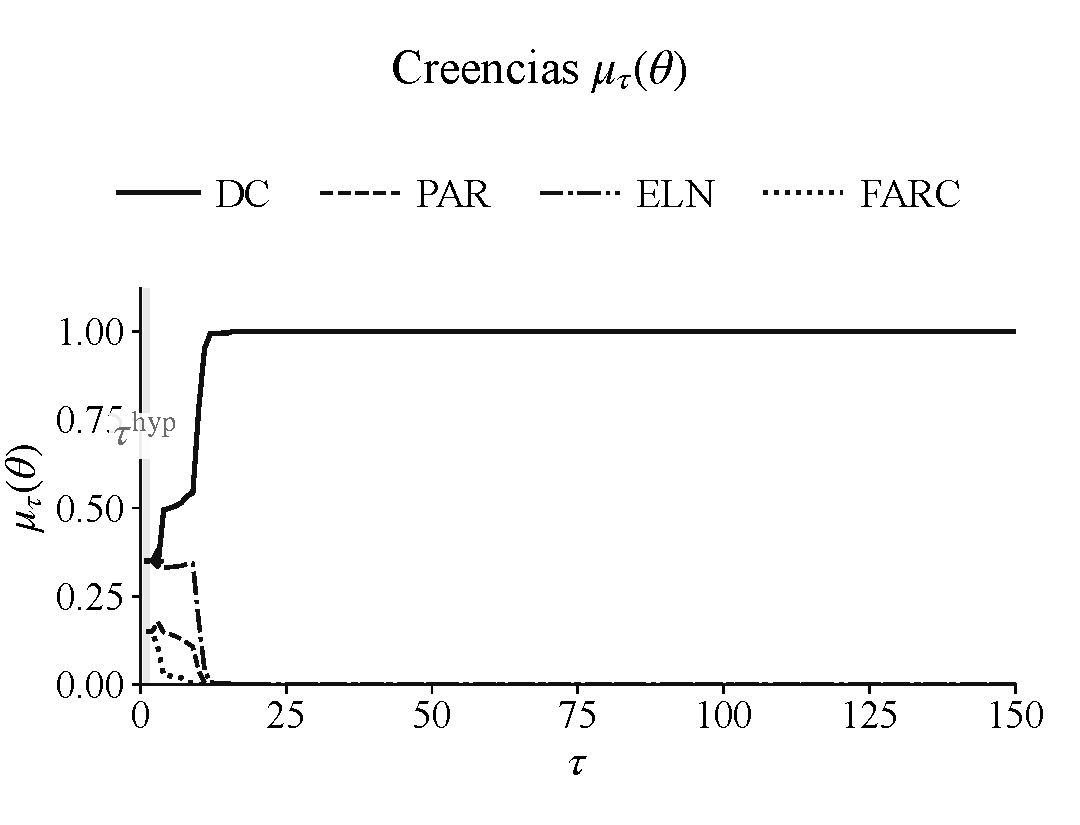
\includegraphics[width=\linewidth]{figuras_calibracion_150/DC_01_mu.pdf}
  \caption{Escenario I: DC}
\end{subfigure}\hfill
\begin{subfigure}[t]{0.48\textwidth}
  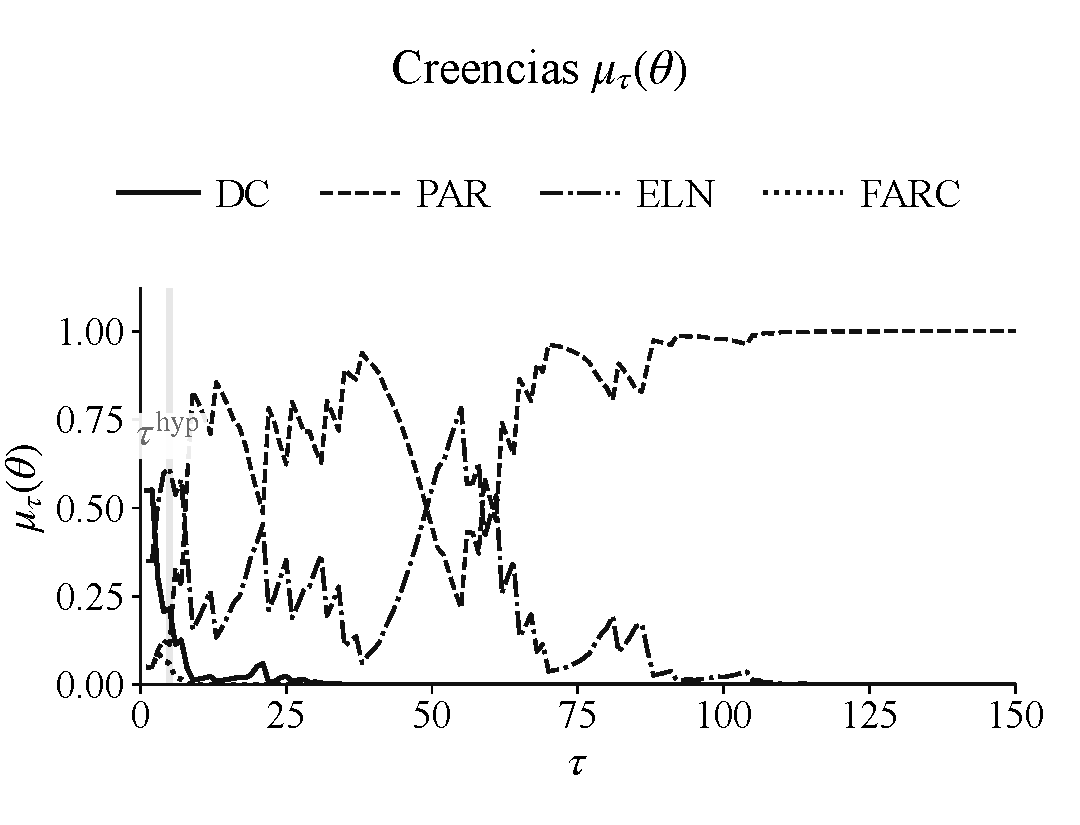
\includegraphics[width=\linewidth]{figuras_calibracion_150/PAR_01_mu.pdf}
  \caption{Escenario II: PAR}
\end{subfigure}

\begin{subfigure}[t]{0.48\textwidth}
  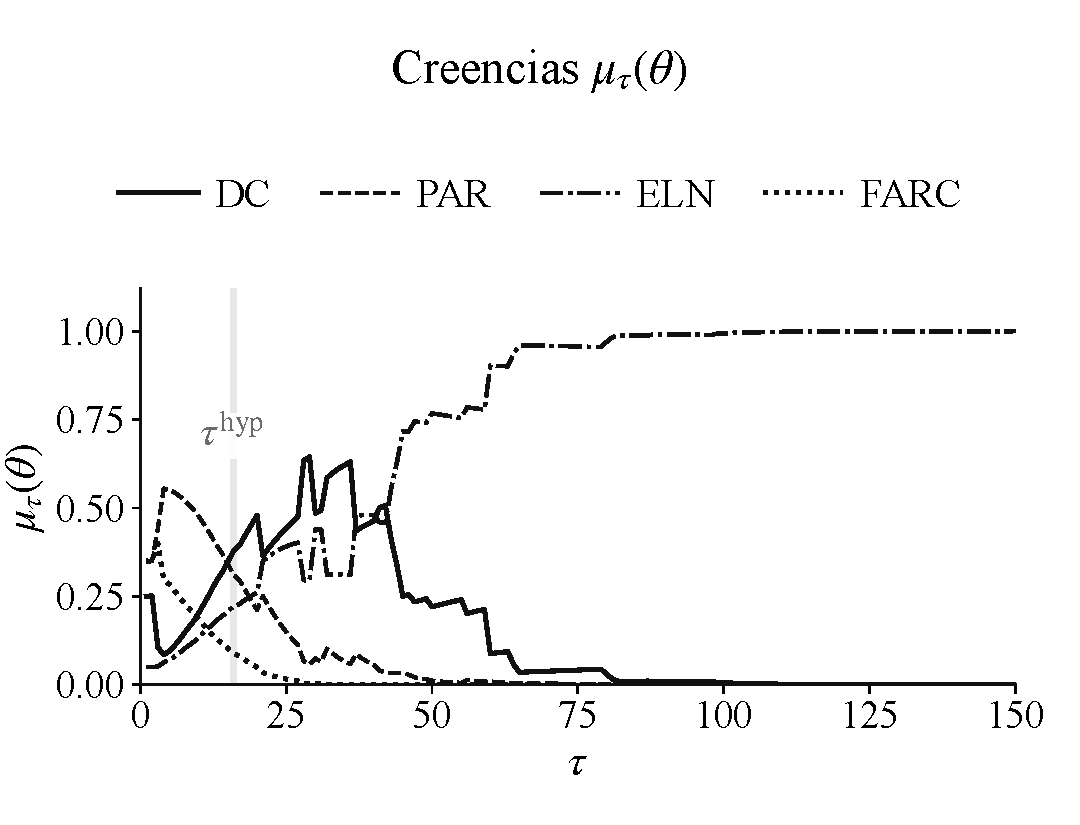
\includegraphics[width=\linewidth]{figuras_calibracion_150/ELN_01_mu.pdf}
  \caption{Escenario III: ELN}
\end{subfigure}\hfill
\begin{subfigure}[t]{0.48\textwidth}
  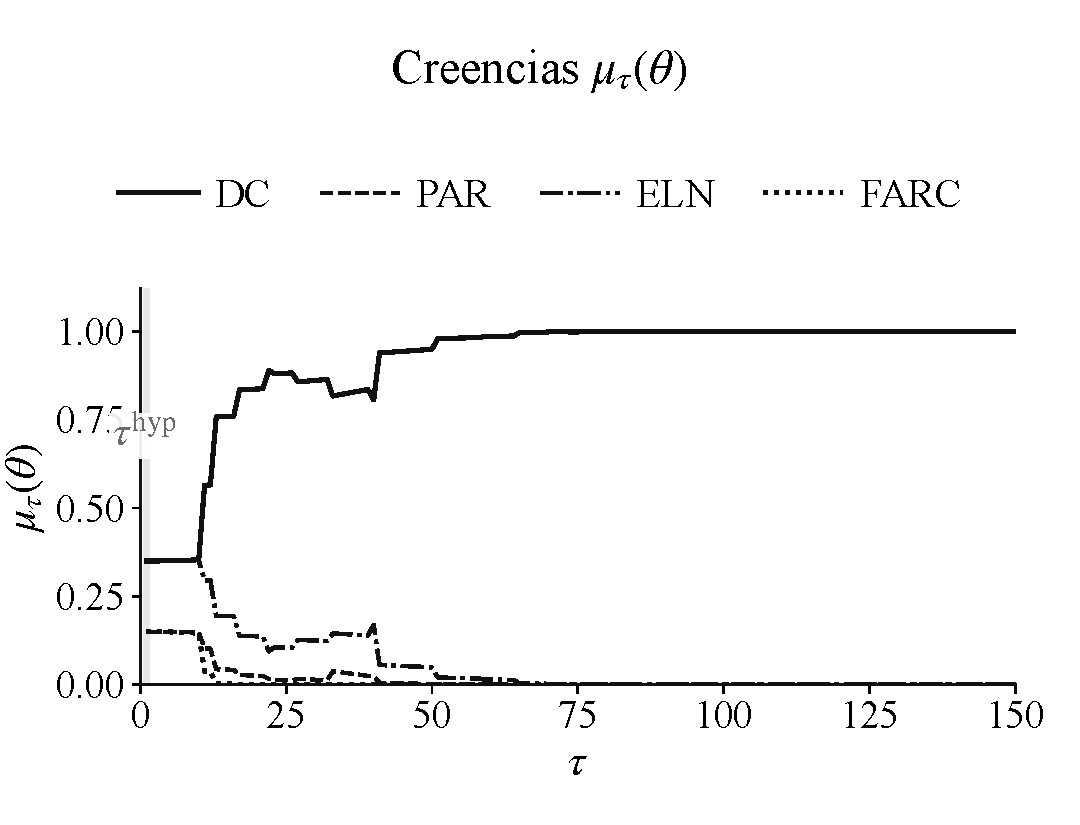
\includegraphics[width=\linewidth]{figuras_calibracion_150/FARC_01_mu.pdf}
  \caption{Escenario IV: FARC}
\end{subfigure}
\caption{Creencias bayesianas para los cuatro tipos de captor, $t\leq150$.}
\label{fig:cal-cuatro-mu}
\caption*{\footnotesize\textit{Nota:} la franja gris indica el primer desenlace distinto de continuar. La trayectoria posterior corresponde a la extensión contrafactual condicionada a la no absorción.}
\end{figure}

\subsection{Presión operativa e interdicción financiera}

La presión operativa promedio es $0{,}804$ en DC, $0{,}871$ en PAR, $0{,}903$ en ELN y $0{,}812$ en FARC. Frente a las referencias de rescate, $\gamma^R=(0{,}80,0{,}86,0{,}92,0{,}80)$, las trayectorias muestran que el Estado no replica mecánicamente una rama pura. La política combina el efecto material de la intervención con el valor esperado de la información, de modo que la intensidad cambia con la posterior y con las condiciones institucionales del episodio.

\begin{figure}[htbp]
\centering
\begin{subfigure}[t]{0.48\textwidth}
  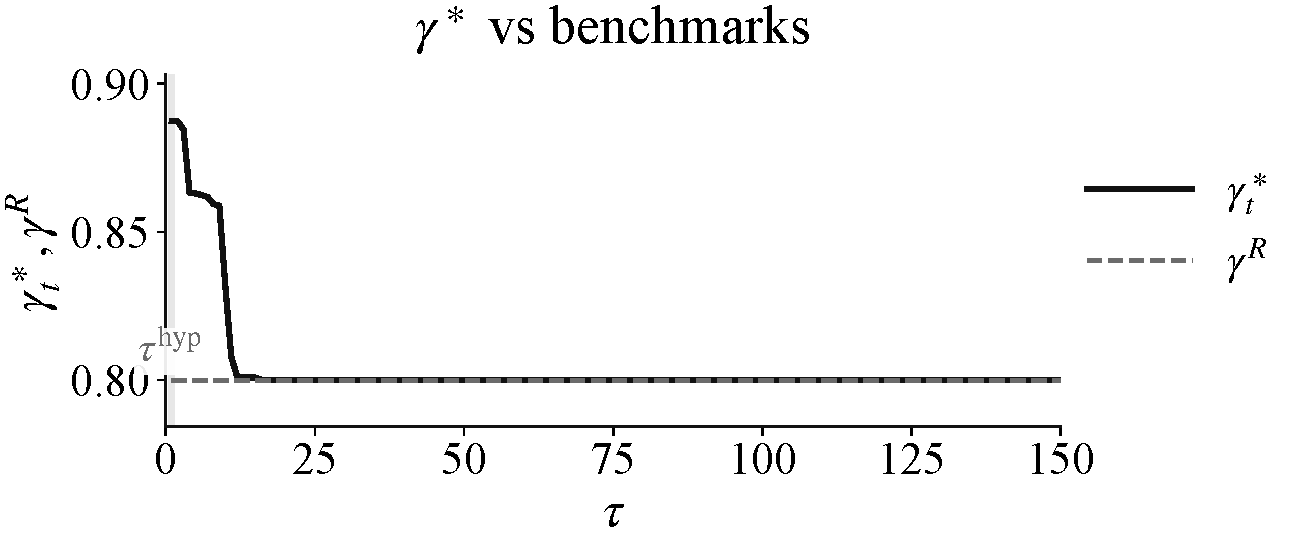
\includegraphics[width=\linewidth]{figuras_calibracion_150/DC_03_gamma.pdf}
  \caption{DC}
\end{subfigure}\hfill
\begin{subfigure}[t]{0.48\textwidth}
  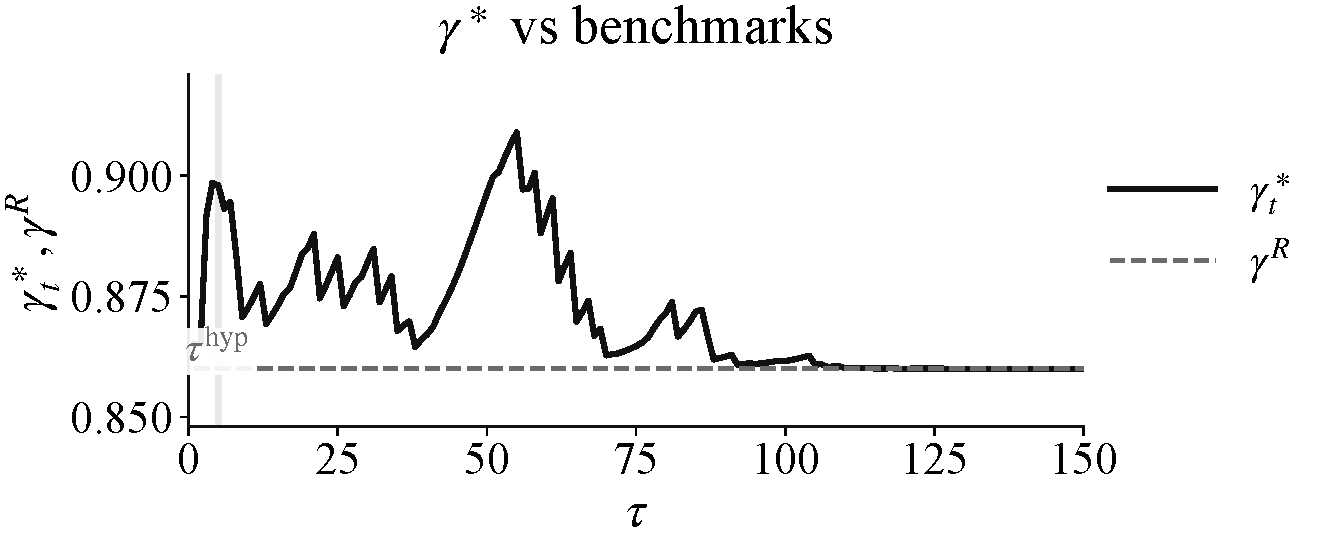
\includegraphics[width=\linewidth]{figuras_calibracion_150/PAR_03_gamma.pdf}
  \caption{PAR}
\end{subfigure}

\begin{subfigure}[t]{0.48\textwidth}
  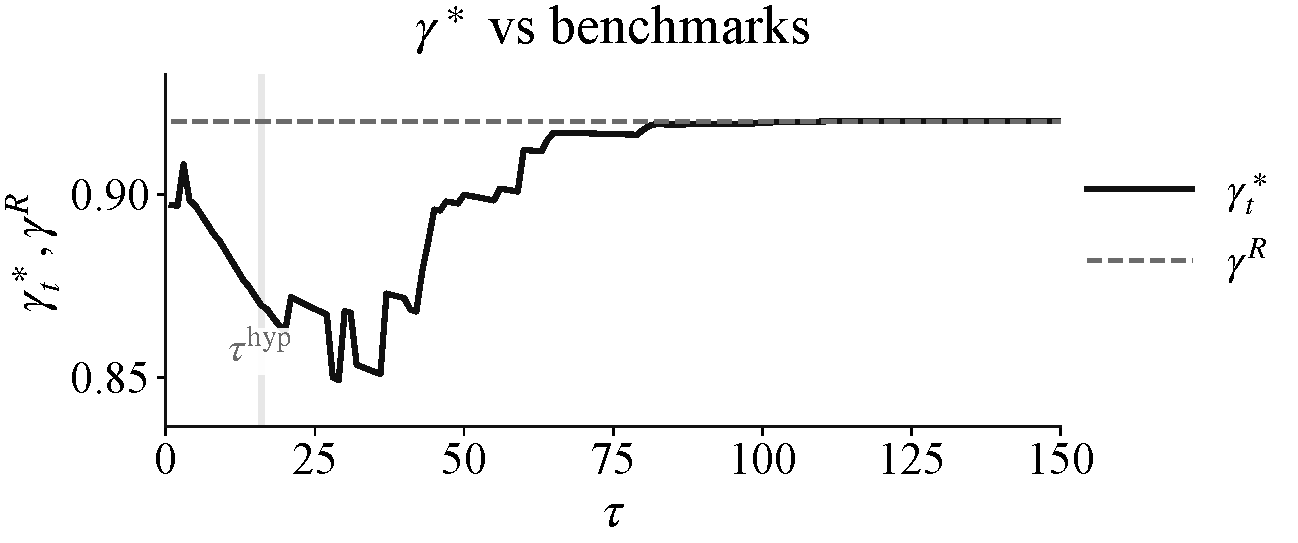
\includegraphics[width=\linewidth]{figuras_calibracion_150/ELN_03_gamma.pdf}
  \caption{ELN}
\end{subfigure}\hfill
\begin{subfigure}[t]{0.48\textwidth}
  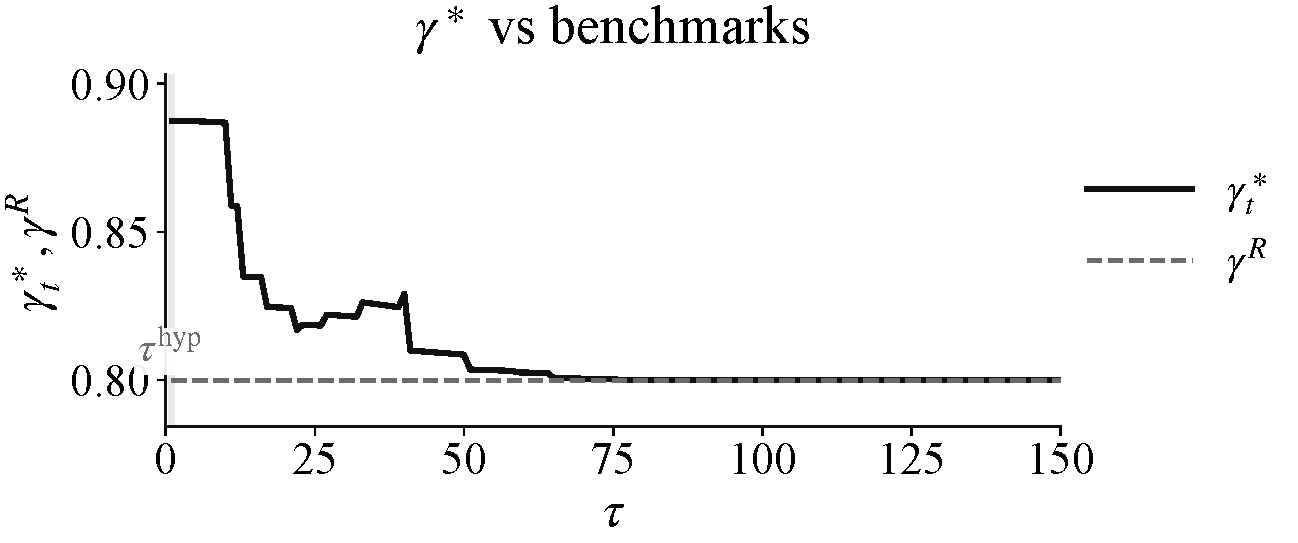
\includegraphics[width=\linewidth]{figuras_calibracion_150/FARC_03_gamma.pdf}
  \caption{FARC}
\end{subfigure}
\caption{Presión operativa óptima $\gamma_t^\ast$ y referencias del mecanismo.}
\label{fig:cal-cuatro-gamma}
\end{figure}

La interdicción financiera promedio es $0{,}790$ en DC, $0{,}921$ en PAR, $0{,}910$ en ELN y $0{,}803$ en FARC. Los valores de referencia de rescate son $\alpha^R=(0{,}78,0{,}84,0{,}90,0{,}78)$. La mayor intensidad media aparece en PAR, donde la combinación de alta riqueza familiar, víctima privada y entorno Oriente--Selva conserva el valor estratégico de restringir pagos. En ELN, el instrumento también permanece elevado, pero opera en un episodio con víctima pública y baja capacidad de pago.

\begin{figure}[htbp]
\centering
\begin{subfigure}[t]{0.48\textwidth}
  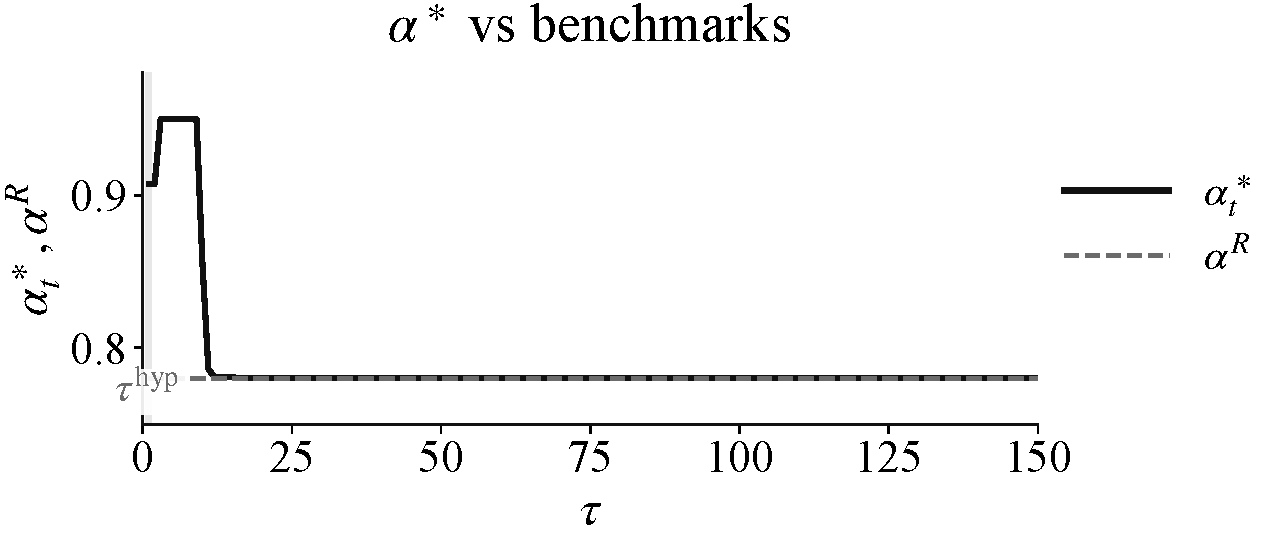
\includegraphics[width=\linewidth]{figuras_calibracion_150/DC_02_alpha.pdf}
  \caption{DC}
\end{subfigure}\hfill
\begin{subfigure}[t]{0.48\textwidth}
  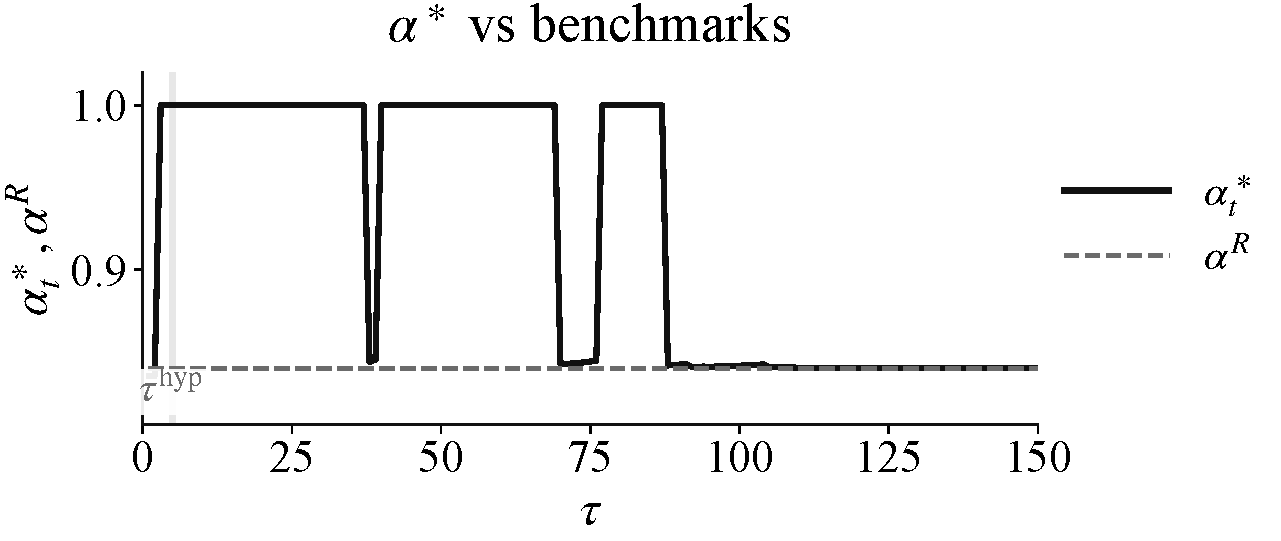
\includegraphics[width=\linewidth]{figuras_calibracion_150/PAR_02_alpha.pdf}
  \caption{PAR}
\end{subfigure}

\begin{subfigure}[t]{0.48\textwidth}
  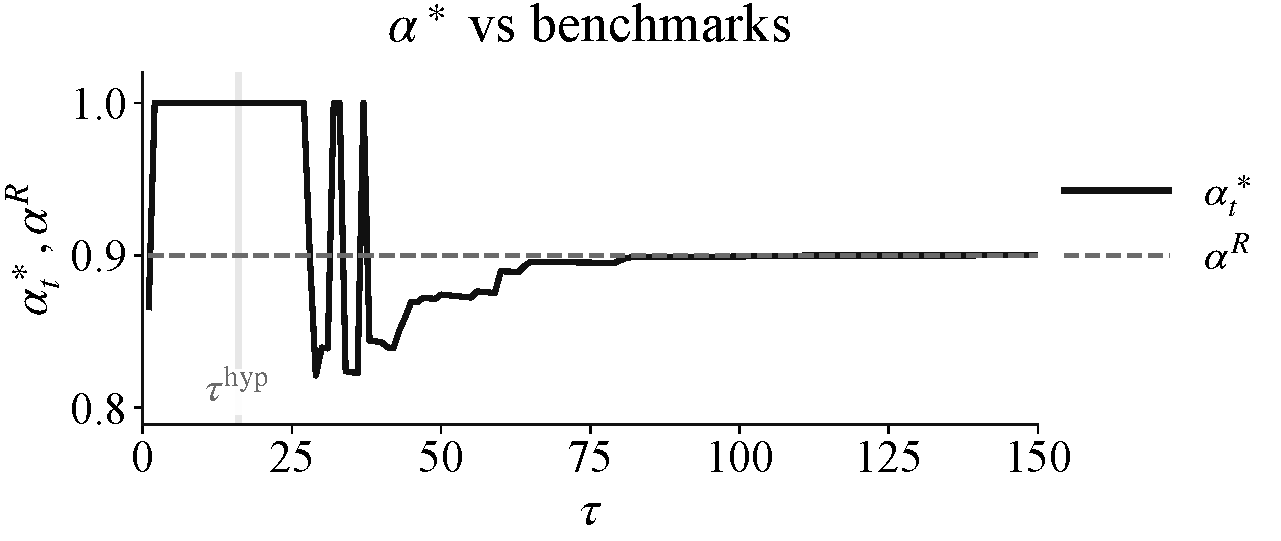
\includegraphics[width=\linewidth]{figuras_calibracion_150/ELN_02_alpha.pdf}
  \caption{ELN}
\end{subfigure}\hfill
\begin{subfigure}[t]{0.48\textwidth}
  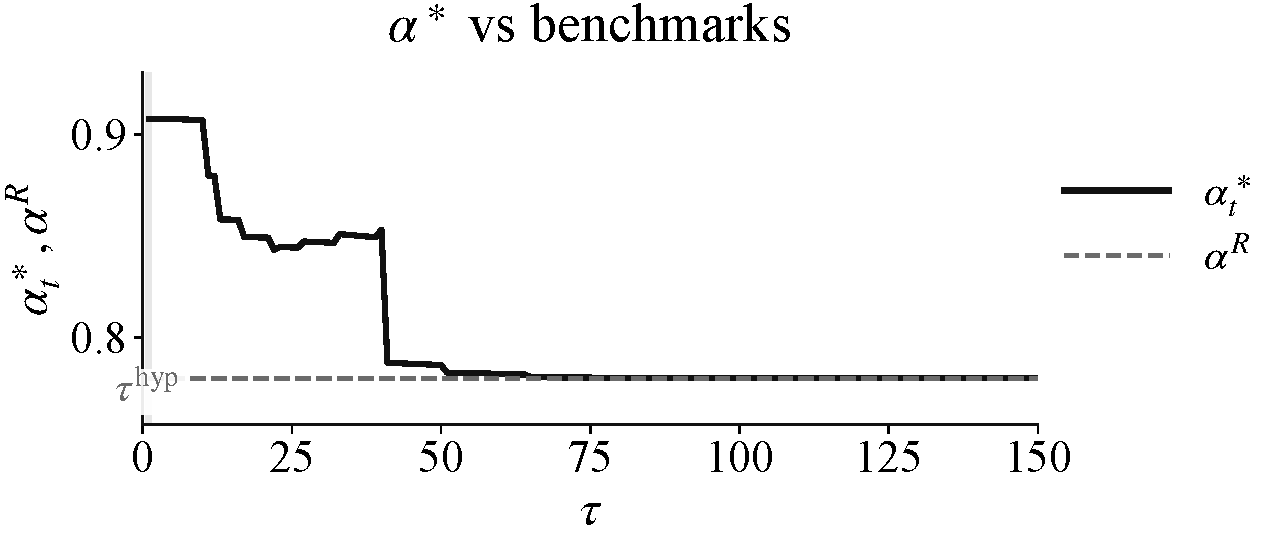
\includegraphics[width=\linewidth]{figuras_calibracion_150/FARC_02_alpha.pdf}
  \caption{FARC}
\end{subfigure}
\caption{Interdicción financiera óptima $\alpha_t^\ast$ y referencias del mecanismo.}
\label{fig:cal-cuatro-alpha}
\end{figure}

\subsection{Ganancia informacional y viabilidad del mecanismo}

La ganancia informacional se concentra en los primeros periodos. Su máximo es $0{,}0381$ en $t=7$ para DC, $0{,}0353$ en $t=6$ para PAR, $0{,}0430$ en $t=10$ para ELN y $0{,}0319$ en $t=10$ para FARC. A medida que $\Delta H_t$ se aproxima a cero, la contribución marginal de nuevas observaciones disminuye y la política queda gobernada principalmente por los costos materiales y la creencia acumulada.

Las verificaciones $IR^K$, $IC^K$ e $IR^F$ se satisfacen en la totalidad de los 150 ciclos de los cuatro escenarios. Este resultado establece viabilidad interna de las trayectorias simuladas, pero no garantiza por sí solo identificación correcta: FARC satisface las restricciones y, sin embargo, sus señales inducen clasificación posterior hacia DC. La distinción confirma que la implementabilidad del mecanismo y la separación estadística de tipos son condiciones relacionadas, pero conceptualmente diferentes.

\begin{figure}[htbp]
\centering
\begin{subfigure}[t]{0.48\textwidth}
  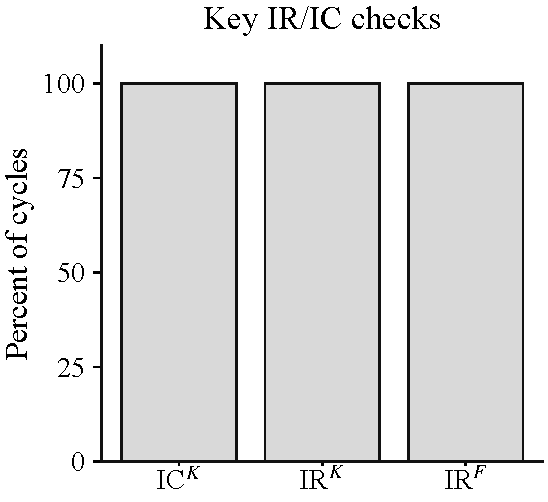
\includegraphics[width=\linewidth]{figuras_calibracion_150/DC_11_IRIC.pdf}
  \caption{DC}
\end{subfigure}\hfill
\begin{subfigure}[t]{0.48\textwidth}
  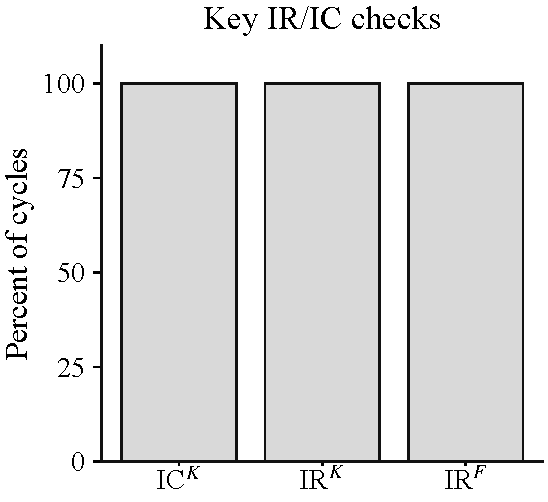
\includegraphics[width=\linewidth]{figuras_calibracion_150/PAR_11_IRIC.pdf}
  \caption{PAR}
\end{subfigure}

\begin{subfigure}[t]{0.48\textwidth}
  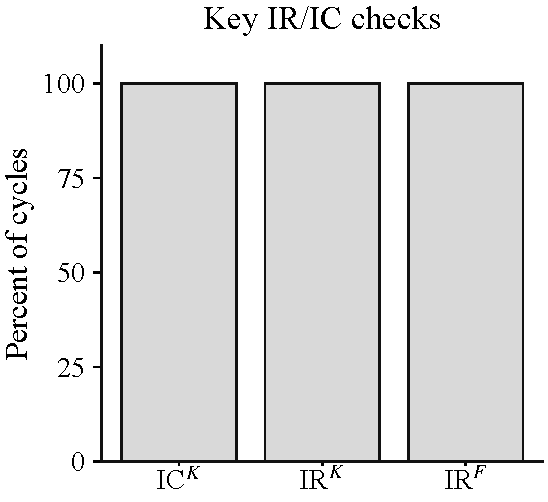
\includegraphics[width=\linewidth]{figuras_calibracion_150/ELN_11_IRIC.pdf}
  \caption{ELN}
\end{subfigure}\hfill
\begin{subfigure}[t]{0.48\textwidth}
  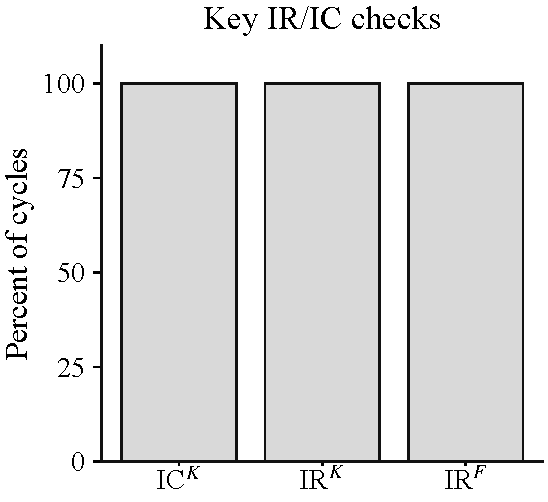
\includegraphics[width=\linewidth]{figuras_calibracion_150/FARC_11_IRIC.pdf}
  \caption{FARC}
\end{subfigure}
\caption{Cumplimiento de las restricciones de participación e incentivos.}
\label{fig:cal-cuatro-iric}
\end{figure}

\subsection{Síntesis cuantitativa}

Los primeros desenlaces terminales ocurren en $t=16$ para DC (rescate), $t=5$ para PAR (muerte), $t=16$ para ELN (liberación) y $t=32$ para FARC (rescate). La Tabla~\ref{tab:calibracion-cuatro} resume los resultados calculados sobre el mismo horizonte de 150 periodos.

\begin{table}[htbp]
\centering
\caption{Resumen de la calibración para los cuatro tipos, $t\leq150$}
\label{tab:calibracion-cuatro}
\begin{tabular}{lcccccl}
\toprule
Escenario & $\mu_1(\theta^\ast)$ & $\mu_{150}(\theta^\ast)$ & $\bar\alpha^\ast$ & $\bar\gamma^\ast$ & $\tau^{\mathrm{hyp}}$ & Desenlace \\
\midrule
DC   & 0,350 & 1,000000 & 0,790 & 0,804 & 16 & Rescate \\
PAR  & 0,050 & 0,999922 & 0,921 & 0,871 & 5  & Muerte \\
ELN  & 0,050 & 0,999911 & 0,910 & 0,903 & 16 & Liberación \\
FARC & 0,150 & 0,000000 & 0,803 & 0,812 & 32 & Rescate \\
\bottomrule
\end{tabular}
\caption*{\footnotesize\textit{Nota:} en FARC la masa posterior se concentra en DC al final del horizonte; por ello, el valor cercano a cero no se interpreta como identificación del tipo verdadero, sino como evidencia de falta de separación bajo esa trayectoria.}
\end{table}

En conjunto, la comparación de los cuatro casos muestra que un mismo mecanismo puede ser implementable y generar políticas diferenciadas, pero la concentración posterior depende de la capacidad informativa de las señales. DC, PAR y ELN producen separación clara a 150 periodos; FARC revela una zona de fragilidad empírica que exige revisar la calibración de verosimilitudes o incorporar señales adicionales antes de sostener identificación robusta para ese tipo.
% SECCIÓN 6, IMPLICACIONES DE POLÍTICA
% ============================================================
\section{Implicaciones de política}
\label{sec:policy-implications}

Los resultados de las secciones anteriores tienen consecuencias directas sobre el diseño de la política antikidnapping. La Proposición~\ref{prop:expected-captivity-gamma} establece que el efecto de $\gamma_t$ sobre la duración esperada del cautiverio está gobernado por el signo de $\kappa_h(\theta_K,t)$: solo cuando la presión acelera los desenlaces de cierre más de lo que inhibe el canal de pago se acorta el episodio; en caso contrario, el Estado puede paradójicamente prolongarlo. La Proposición~\ref{prop:optimal-gamma-beliefs} traduce esta heterogeneidad a una regla de calibración bayesiana: el Estado utiliza la actualización de \textit{Bayes} para disciplinar su política, de modo que a medida que la evidencia $(\mathcal{I}_t)$ incrementa el peso sobre el tipo de alto riesgo, el planificador intensifica $\gamma_t^\ast$ para explotar esa sensibilidad y forzar un cierre temprano. La magnitud de la respuesta es proporcional a la separación estructural $\beta_{K,j}(\theta_{high})-\beta_{K,j}(\theta_{low})$, que actúa como amplificador de la política ante la llegada de nueva información.

\begin{proposition}[Presión operativa óptima e identificación bayesiana del tipo]
\label{prop:optimal-gamma-beliefs}
Supóngase $\Theta_K=\{\theta_{low},\theta_{high}\}$ con $\beta_{K,j}(\theta_{high})>\beta_{K,j}(\theta_{low})$ para $j\in\{2,3\}$ \textup{(}el tipo de alto riesgo exhibe mayor propensión a rescate y muerte\textup{)}, y que el objetivo del Estado~\eqref{eq:state-expected-loss} es estrictamente convexo en $\gamma_t$ en el interior de $\Gamma_t(\mu_t)$. Entonces la presión operativa óptima $\gamma_t^\ast$ es estrictamente creciente en la creencia posterior sobre el tipo de alto riesgo:
\[
\frac{d\gamma_t^\ast}{d\mu_t(\theta_{high})} > 0.
\]
La elasticidad de $\gamma_t^\ast$ respecto a $\mu_t(\theta_{high})$ depende del cociente diferencial de pérdidas marginales entre tipos, que a su vez es proporcional a
\[
\frac{\tilde\lambda_j(t\mid\theta_{high})}{\tilde\lambda_j(t\mid\theta_{low})}
= \exp\!\bigl(\beta_{K,j}(\theta_{high})-\beta_{K,j}(\theta_{low})\bigr), \quad j\in\{2,3\}.
\]
En consecuencia, el rango de variación de la presión óptima ante actualizaciones bayesianas es mayor cuanto más separados estén los parámetros estructurales $\beta_{K,j}$ entre tipos.
\end{proposition}

\begin{proof}
La prueba procede en cuatro pasos: construcción del programa del Estado,
condición de primer orden, aplicación del teorema de la función implícita
y derivación de la elasticidad estructural.

\paragraph{Paso 1. Programa del Estado y condición de interior.}
Con $\Theta_K=\{\theta_{low},\theta_{high}\}$ y
$\mu_t(\theta_{low})=1-\mu_t(\theta_{high})$, el objetivo del
Estado~\eqref{eq:state-expected-loss} respecto a $\gamma_t$, fijados $\mu_t$
y los demás instrumentos, se reduce a
\begin{equation}
\label{eq:obj-gamma}
\mathcal{W}(\gamma_t,\mu_t)
:= \mu_t(\theta_{high})\,L_t(\gamma_t,\theta_{high})
 + \bigl(1-\mu_t(\theta_{high})\bigr)\,L_t(\gamma_t,\theta_{low})
 + \chi_\gamma\bigl(\gamma_t-\gamma_t^\mu\bigr)^2.
\end{equation}
Por la hipótesis de convexidad estricta en $\gamma_t$ sobre el interior de
$\Gamma_t(\mu_t)$, la función $\mathcal{W}$ tiene un único minimizador interior
$\gamma_t^\ast(\mu_t)$ que satisface la condición de primer orden
\begin{equation}
\label{eq:foc-gamma}
\Phi(\gamma_t,\mu_t)
:= \mu_t(\theta_{high})\,\frac{\partial L_t}{\partial\gamma_t}(\theta_{high})
 + \bigl(1-\mu_t(\theta_{high})\bigr)\,
   \frac{\partial L_t}{\partial\gamma_t}(\theta_{low})
 + 2\chi_\gamma\bigl(\gamma_t-\gamma_t^\mu\bigr)
= 0,
\end{equation}
con $\partial\Phi/\partial\gamma_t = \partial^2\mathcal{W}/\partial\gamma_t^2 > 0$
en el interior de $\Gamma_t(\mu_t)$ por convexidad estricta.

\paragraph{Paso 2. Teorema de la función implícita.}
Como $\Phi(\gamma_t^\ast,\mu_t)=0$ y $\partial\Phi/\partial\gamma_t>0$,
el teorema de la función implícita garantiza que $\gamma_t^\ast$ es una función
continuamente diferenciable de $\mu_t(\theta_{high})$ en un entorno del óptimo,
con derivada
\begin{equation}
\label{eq:tfi}
\frac{d\gamma_t^\ast}{d\mu_t(\theta_{high})}
= -\frac{\partial\Phi/\partial\mu_t(\theta_{high})}
        {\partial\Phi/\partial\gamma_t}
= -\frac{
    \dfrac{\partial L_t}{\partial\gamma_t}(\theta_{high})
    -\dfrac{\partial L_t}{\partial\gamma_t}(\theta_{low})
  }{
    \partial\Phi/\partial\gamma_t
  }.
\end{equation}
Dado que el denominador es estrictamente positivo, el signo de~\eqref{eq:tfi}
queda determinado por el signo de la diferencia de pérdidas marginales en el
numerador.

\paragraph{Paso 3. Signo de la diferencia de pérdidas marginales.}
Bajo riesgos proporcionales, $L_t(\gamma_t,\theta_K)$ depende de $\gamma_t$ a
través de las intensidades efectivas
$\tilde{\lambda}_j(t\mid\theta_K)=\lambda_{j0}(t)
\exp\!\bigl(\beta_{K,j}(\theta_K)\cdot z+\zeta_{\gamma,j}\,\gamma_t\bigr)$.
Diferenciando y formando la diferencia entre tipos,
\begin{align}
\label{eq:diff-dL}
\frac{\partial L_t}{\partial\gamma_t}(\theta_{high})
-\frac{\partial L_t}{\partial\gamma_t}(\theta_{low})
&= \sum_{j\in\{2,3\}}\frac{\partial L_t}{\partial\tilde{\lambda}_j}\,
   \zeta_{\gamma,j}\,
   \Bigl[\tilde{\lambda}_j(t\mid\theta_{high})
         -\tilde{\lambda}_j(t\mid\theta_{low})\Bigr] \notag\\
&\quad
 + \frac{\partial L_t}{\partial\tilde{\lambda}_1}\,\zeta_{\gamma,1}\,
   \Bigl[\tilde{\lambda}_1(t\mid\theta_{high})
         -\tilde{\lambda}_1(t\mid\theta_{low})\Bigr].
\end{align}
La razón de hazards entre tipos para $j\in\{2,3\}$ satisface
\begin{equation}
\label{eq:hazard-ratio}
\frac{\tilde{\lambda}_j(t\mid\theta_{high})}
     {\tilde{\lambda}_j(t\mid\theta_{low})}
= \exp\!\Bigl(\beta_{K,j}(\theta_{high})-\beta_{K,j}(\theta_{low})\Bigr)
> 1,
\end{equation}
de modo que $\tilde{\lambda}_j(t\mid\theta_{high})>\tilde{\lambda}_j(t\mid\theta_{low})$
para $j\in\{2,3\}$. Como $\partial L_t/\partial\tilde{\lambda}_j<0$ para
$j\in\{2,3\}$ ---incrementar el hazard de muerte o rescate reduce la pérdida
esperada al acortar el cautiverio--- y $\zeta_{\gamma,j}>0$ para $j\in\{2,3\}$,
el primer término de~\eqref{eq:diff-dL} es estrictamente negativo. Por la hipótesis
$\beta_{K,j}(\theta_{high})>\beta_{K,j}(\theta_{low})$ para $j\in\{2,3\}$, este
diferencial domina sobre el efecto del canal de pago ($j=1$), de modo que la
diferencia en~\eqref{eq:diff-dL} es negativa.

\paragraph{Paso 4. Conclusión y elasticidad estructural.}
Sustituyendo en~\eqref{eq:tfi}, el numerador es negativo y el denominador
positivo, luego $d\gamma_t^\ast/d\mu_t(\theta_{high})>0$. La magnitud de este
ajuste es proporcional a la separación entre las intensidades del tipo de alto
riesgo y del tipo de bajo riesgo, cuantificada por el cociente~\eqref{eq:hazard-ratio}:
a mayor separación $\beta_{K,j}(\theta_{high})-\beta_{K,j}(\theta_{low})$, mayor
es la diferencia en $\partial L_t/\partial\gamma_t$ entre tipos y, por tanto,
mayor la respuesta óptima de $\gamma_t^\ast$ ante actualizaciones bayesianas.
\end{proof}

\subsection{Recomendaciones de política}

\paragraph{Integrar alertas macrofinancieras en la planeación operativa.}
La cointegración entre secuestro extorsivo, capacidad coercitiva y condiciones financieras indica que los cambios en liquidez y costo del capital pueden modificar la cartera criminal. Los sistemas de alerta temprana de las unidades GAULA deberían incorporar indicadores regionales de crédito, liquidez y presión financiera para anticipar cambios en la duración y rentabilidad esperada del secuestro.

\paragraph{Aplicar de forma adaptativa la interdicción financiera.}
El bloqueo $\alpha_t^ast$ disciplina la participación del captor y reduce el espacio para acuerdos clandestinos, pero su aplicación indiscriminada puede imponer costos innecesarios a la familia. La severidad de la interdicción debe responder al tipo posterior, al perfil de la víctima y a la riqueza familiar. Cuando la posterior se concentra y disminuye el valor marginal de experimentar, el bloqueo puede moderarse sin abandonar la trazabilidad financiera ni la capacidad disuasiva.

\paragraph{Adoptar protocolos de inteligencia basados en control dual bayesiano.}
La presión operativa $\gamma_t^ast$ debe perseguir simultáneamente el cierre seguro del episodio y la separación de verosimilitudes entre organizaciones. La combinación sistemática de señales de detección, pruebas de supervivencia, duración del cautiverio y patrones de riesgos competitivos permite clasificar tempranamente al captor, asignar mejor los recursos tácticos y reducir el riesgo humano de las operaciones.


% ============================================================
% SECCIÓN 6, IDENTIFICACIÓN ESTRUCTURAL: SINGULARIDAD DE MEDIDAS
% ============================================================
\section{Identificación estructural: singularidad de medidas}
\label{app:general-id}

Esta sección presenta, en un marco abstracto acorde con la Sección~\ref{sec:asymptotic-learning} y el Lema~\ref{lem:hazard-separation}, por qué la \textbf{separación local recurrente} en variación total entre leyes diarias se acopla al criterio de \textcite{Kakutani1948} para obtener \textbf{singularidad mutua} de las leyes de trayectorias. El evento de cautiverio prolongado $\mathcal{T}$ \textup{(}Definición~\ref{def:event-T-long}\textup{)} es un subconjunto de $\Omega$; los índices temporales son $t\in\{0,1,2,\ldots\}$.

\medskip\noindent\textbf{Notación \textup{(}alineada con el cuerpo del texto\textup{)}.}
Fijada una trayectoria de política $\chi$ compatible con el EBP, sea $Y_t=(m_t,d_t)$ el registro público diario y sea $p_\theta^{(t)}$ la función de masa de $Y_t$ condicionada a la información pública al abrir $t$ bajo el tipo $\theta$ \textup{(}misma lógica que $p_\theta(\cdot\mid\mathcal{F}_t^{\mathrm{pub}})$ en el Lema~\ref{lem:hazard-separation}\textup{)}. Para dos masas $p,q$ en el mismo soporte finito, la \textbf{afinidad} \textup{(}coeficiente de Bhattacharyya\textup{)} es $\rho(p,q):=\sum_y \sqrt{p(y)q(y)}$; la distancia de Hellinger al cuadrado adopta aquí la normalización
\[
\mathsf{H}^2(p,q):=\frac{1}{2}\sum_y\bigl(\sqrt{p(y)}-\sqrt{q(y)}\bigr)^2 = 1-\rho(p,q).
\]
La distancia en variación total cumple $\|p-q\|_{\mathrm{TV}}=\tfrac{1}{2}\sum_y|p(y)-q(y)|$ \textup{(}como en \eqref{eq:TV-separation}\textup{)}.

\begin{lemma}[Producto de experimentos y singularidad \textup{(}criterio de Kakutani\textup{)}]
\label{lem:general-id-appendix}
Fijados dos tipos $\theta\neq\theta'$, supóngase que, condicionada a la política fijada en el equilibrio y al régimen de comparación relevante \textup{(}en particular, al evento $\mathcal{T}$ cuando se trabaje con cautiverio prolongado\textup{)}, la sucesión de experimentos diarios $\{Y_t\}_{t\ge 0}$ es independiente y cada $Y_t$ toma valores en un soporte finito común $\mathcal{Y}_t$. Es decir, para cada horizonte finito $T$, la ley de la trayectoria $(Y_0,\ldots,Y_T)$ factoriza como medida producto $\bigotimes_{t=0}^{T} p_\theta^{(t)}$ bajo el tipo $\theta$, y análogamente como $\bigotimes_{t=0}^{T} p_{\theta'}^{(t)}$ bajo $\theta'$, donde $p_\theta^{(t)}$ y $p_{\theta'}^{(t)}$ son funciones de masa sobre el mismo $\mathcal{Y}_t$. Sea $\rho_t:=\rho\bigl(p_\theta^{(t)},p_{\theta'}^{(t)}\bigr)$. Entonces la afinidad entre las leyes producto en el horizonte $T$ es
\begin{equation}
\label{eq:appendix-rho-product}
\rho\Bigl(\bigotimes_{t=0}^{T} p_\theta^{(t)},\,\bigotimes_{t=0}^{T} p_{\theta'}^{(t)}\Bigr)=\prod_{t=0}^{T}\rho_t.
\end{equation}
Si existe un conjunto infinito de periodos $\mathcal{S}_{\theta,\theta'}\subseteq\mathbb{N}$ tal que $\|p_\theta^{(t)}-p_{\theta'}^{(t)}\|_{\mathrm{TV}}\ge \underline{\varepsilon}>0$ para todo $t\in\mathcal{S}_{\theta,\theta'}$, entonces $\rho_t\le 1-\underline{\varepsilon}^{\,2}/2$ para todo $t\in\mathcal{S}_{\theta,\theta'}$ y, por tanto, $\prod_{t\in\mathcal{S}_{\theta,\theta'}}\rho_t=0$. En el límite $T\to\infty$, el criterio de \textcite{Kakutani1948} implica que las medidas producto sobre la sucesión infinita son \textbf{mutuamente singulares} \textcite{Shiryaev2019Probability}. En particular, cuando la factorización anterior se formula bajo la ley condicionada o restringida al evento $\mathcal{T}$, estas son precisamente las leyes de $\{Y_t\}_{t\ge 0}$ relevantes para la singularidad cola de la Definición~\ref{def:asymptotic-id}\textup{(b)}.
\end{lemma}

\begin{proof}
La identidad~\eqref{eq:appendix-rho-product} se obtiene expandiendo las masas de las trayectorias finitas. En efecto, bajo independencia,
\[
\rho\Bigl(\bigotimes_{t=0}^{T} p_\theta^{(t)},\,\bigotimes_{t=0}^{T} p_{\theta'}^{(t)}\Bigr)
=\sum_{(y_0,\ldots,y_T)}\prod_{t=0}^{T}\sqrt{p_\theta^{(t)}(y_t)p_{\theta'}^{(t)}(y_t)}
=\prod_{t=0}^{T}\sum_{y_t\in\mathcal{Y}_t}\sqrt{p_\theta^{(t)}(y_t)p_{\theta'}^{(t)}(y_t)}.
\]
Para la segunda parte, usamos la desigualdad estándar $\|p-q\|_{\mathrm{TV}}\le \sqrt{2}\,\mathsf{H}(p,q)$ en espacios finitos. Como $\mathsf{H}^2(p,q)=1-\rho(p,q)$ con la normalización adoptada, si $\|p-q\|_{\mathrm{TV}}\ge\underline{\varepsilon}$ entonces
\[
\rho(p,q)\le 1-\frac{\underline{\varepsilon}^{\,2}}{2}.
\]
Así, en cada $t\in\mathcal{S}_{\theta,\theta'}$ se tiene $\rho_t\le 1-\underline{\varepsilon}^{\,2}/2<1$. Al haber infinitos periodos en $\mathcal{S}_{\theta,\theta'}$, el producto de afinidades contiene infinitos factores uniformemente acotados por debajo de $1$, luego $\prod_{t\in\mathcal{S}_{\theta,\theta'}}\rho_t=0$. Por el criterio de \textcite{Kakutani1948} para productos de probabilidades, las medidas producto infinitas asociadas son mutuamente singulares \textcite{Shiryaev2019Probability}. La lectura respecto de la Definición~\ref{def:asymptotic-id} y la convergencia posterior bajo las hipótesis del Teorema~\ref{thm:posterior-consistency} se completan en el cuerpo del texto \textup{(}no se repite aquí el paso bayesiano para no duplicar la prueba\textup{)}.
\end{proof}

\medskip
\paragraph{Versión general del Teorema~\ref{thm:posterior-consistency}.}
El Lema~\ref{lem:general-id-appendix} aísla el argumento \emph{puro} de teoría de la medida, bajo estructura producto y separación recurrente en variación total, el criterio de \textcite{Kakutani1948} fuerza \textbf{singularidad mutua} de las leyes de trayectorias. El Teorema~\ref{thm:posterior-consistency} en el cuerpo del texto invoca la identificación asintótica \textup{(}Definición~\ref{def:asymptotic-id}\textup{)} y, como vía suficiente verificable, el Lema~\ref{lem:hazard-separation}. El resultado siguiente enuncia la misma conclusión bayesiana sustituyendo esa vía por las hipótesis del Lema~\ref{lem:general-id-appendix} sobre el experimento diario $Y_t$ \textup{(}reducción alineada con la notación del anexo y con el bloque operativo de $(m_t,d_t)$\textup{)}; en particular, el Teorema~\ref{thm:posterior-consistency} es el caso en el que dichas hipótesis se obtienen del mecanismo vía el Lema~\ref{lem:hazard-separation}.

\begin{theorem}[Consistencia posterior bajo singularidad de medidas producto \textup{(}criterio de Kakutani\textup{)}]
\label{thm:posterior-consistency-appendix}
Suponga $\Theta_K$ finito, prior $\mu_0$ con soporte total y actualización bayesiana consistente con el EBP \textup{(}Definición~\ref{def:beliefs-martingale}\textup{)}. Sea $\theta_K^\ast$ el tipo realizado y $\mathcal{T}$ el evento de cautiverio prolongado \textup{(}Definición~\ref{def:event-T-long}\textup{)}. Suponga que, para todo $\theta\in\Theta_K$ con $\theta\neq\theta_K^\ast$, valen las siguientes condiciones.
\begin{enumerate}
  \item[\textup{(i)}] \textbf{Compatibilidad de trayectorias.} $\ProbC{\theta_K^\ast}(\mathcal{T})>0$ y, para cada tipo falso, o bien $\ProbC{\theta}(\mathcal{T})=0$ \textup{(}exclusión por supervivencia\textup{)}, o bien las leyes de señales se comparan bajo la ley condicionada/restringida a $\mathcal{T}$ como en los incisos siguientes.
  \item[\textup{(ii)}] \textbf{Producto y separación recurrente en TV.} para todo tipo falso con $\ProbC{\theta}(\mathcal{T})>0$, condicionada a la política fijada por el equilibrio y al evento $\mathcal{T}$, la sucesión $\{Y_t\}_{t\ge 0}$ satisface la factorización producto y la existencia de $\mathcal{S}_{\theta,\theta_K^\ast}$ y $\underline{\varepsilon}_\theta>0$ descritas en el Lema~\ref{lem:general-id-appendix} \textup{(}mismas notaciones $p_\theta^{(t)}$, $p_{\theta_K^\ast}^{(t)}$\textup{)}.
  \item[\textup{(iii)}] \textbf{Alineación señal-experimento.} en $\mathcal{T}$, la componente de la señal pública $\zeta_t$ contiene $Y_t=(m_t,d_t)$; como $Y_t$ es $\sigma(\zeta_t)$-medible, se tiene $\sigma(\{Y_t\}_{t\ge 0})\subseteq\sigma(\{\zeta_t\}_{t\ge 0})$ y, por monotonía de la singularidad mutua respecto a $\sigma$-álgebras \textup{(}si dos leyes son singulares en una sub-$\sigma$-álgebra, siguen siéndolo al considerarlas en una $\sigma$-álgebra mayor que contiene el evento separador; véase \textcite{Shiryaev2019Probability,Schervish1995Theory}\textup{)}, la singularidad mutua de las leyes de $\{Y_t\}_{t\ge 0}$ se traslada a la de $\{\zeta_t\}_{t\ge 0}$, en el sentido de la parte~\textup{(b)} de la Definición~\ref{def:asymptotic-id}.
\end{enumerate}
Entonces, en el régimen $\mathcal{T}$, se cumplen simultáneamente
\[
\mu_t(\theta)\xrightarrow[t\to\infty]{}0
\qquad
\forall\,\theta\neq\theta_K^\ast,
\qquad
\ProbC{\theta_K^\ast}\textup{-c.s. en }\mathcal{T},
\]
y
\[
\mu_t(\theta_K^\ast)\xrightarrow[t\to\infty]{}1
\qquad \ProbC{\theta_K^\ast}\textup{-c.s. en }\mathcal{T}.
\]
Equivalentemente, en $\mathcal{T}$ la sucesión $\{\mu_t\}$ converge débilmente, $\ProbC{\theta_K^\ast}$-c.s., a $\delta_{\theta_K^\ast}$.
\textup{(}En el caso estricto en que $\ProbC{\theta}(\mathcal{T})=0$ para todo $\theta\neq\theta_K^\ast$, la conclusión se lee además como aplicación directa de la Definición~\ref{def:asymptotic-id}; cuando algún tipo falso tiene masa positiva en $\mathcal{T}$, los incisos~\textup{(ii)}--\textup{(iii)} sustituyen la exclusión por supervivencia mediante singularidad de señales.\textup{)}
\end{theorem}

\begin{proof}
Fijemos $\theta\neq\theta_K^\ast$. Primero probamos que la posterior del tipo falso converge a cero. Si $\ProbC{\theta}(\mathcal{T})=0$, el régimen de comparación $\mathcal{T}$ no ocurre bajo el tipo falso, mientras que $\ProbC{\theta_K^\ast}(\mathcal{T})>0$ por \textup{(i)}. Por tanto, en la ley verdadera restringida a $\mathcal{T}$, el tipo falso queda descartado por supervivencia diferencial y su verosimilitud posterior se anula.

Supongamos ahora que $\ProbC{\theta}(\mathcal{T})>0$. Por \textup{(ii)}, las leyes de $\{Y_t\}_{t\ge0}$ factorizan como producto y presentan separación recurrente en variación total. El Lema~\ref{lem:general-id-appendix} implica que las leyes producto infinitas inducidas por $\theta$ y por $\theta_K^\ast$ son mutuamente singulares. Por \textup{(iii)}, esa singularidad se transfiere al flujo público $\{\zeta_t\}_{t\ge0}$ que alimenta la actualización bayesiana. Así, existe un evento de cola $A_\theta$ tal que
\[
\ProbC{\theta_K^\ast}(A_\theta\mid\mathcal{T})=1,
\qquad
\ProbC{\theta}(A_\theta\mid\mathcal{T})=0.
\]
Sea
\[
R_t^\theta
:=
\frac{d\,\ProbC{\theta}\!\mid_{\mathcal{F}_t^{\mathrm{pub}},\,\mathcal{T}}}
     {d\,\ProbC{\theta_K^\ast}\!\mid_{\mathcal{F}_t^{\mathrm{pub}},\,\mathcal{T}}}
\]
la razón de verosimilitud finita del tipo falso frente al verdadero, definida respecto de la mezcla bayesiana con prior de soporte total. La singularidad de cola fuerza $R_t^\theta\to0$ $\ProbC{\theta_K^\ast}$-c.s. en $\mathcal{T}$ \textcite{BlackwellDubins1962,Schervish1995Theory}. Por Bayes,
\[
\mu_t(\theta)
=
\frac{\mu_0(\theta)R_t^\theta}
{\mu_0(\theta_K^\ast)+\sum_{\theta'\neq\theta_K^\ast}\mu_0(\theta')R_t^{\theta'}}
\le
\frac{\mu_0(\theta)}{\mu_0(\theta_K^\ast)}R_t^\theta,
\]
y como $\mu_0(\theta_K^\ast)>0$, se obtiene
\[
\mu_t(\theta)\to0
\qquad \ProbC{\theta_K^\ast}\text{-c.s. en }\mathcal{T}.
\]
Como $\theta\neq\theta_K^\ast$ era arbitrario y $\Theta_K$ es finito, todas las coordenadas falsas convergen a cero simultáneamente fuera de un conjunto nulo finito.

Finalmente, para todo $t$ se tiene $\sum_{\theta\in\Theta_K}\mu_t(\theta)=1$. Al pasar al límite en la suma finita,
\[
1=\lim_{t\to\infty}\sum_{\theta\in\Theta_K}\mu_t(\theta)
=\lim_{t\to\infty}\mu_t(\theta_K^\ast)
+\sum_{\theta\neq\theta_K^\ast}0,
\]
de modo que $\mu_t(\theta_K^\ast)\to1$ $\ProbC{\theta_K^\ast}$-c.s. en $\mathcal{T}$. En un simplejo finito, la convergencia de todas las coordenadas a las de $\delta_{\theta_K^\ast}$ equivale a convergencia débil.
\end{proof}

% ============================================================
% SECCIÓN 7, CONCLUSIÓN
% ============================================================
\section{Conclusión}
\label{sec:conclusion}

Este trabajo presenta un mecanismo dinámico de disuasión bajo información incompleta para el análisis del secuestro extorsivo, cuya contribución central es el \textbf{Teorema de Identificación de Tipos Racionales bajo Entornos Desconocidos} (Teorema~\ref{thm:posterior-consistency}). El resultado establece que, cuando la política pública genera intensidades de riesgo asintóticamente separables entre tipos de captor, la acumulación de señales diarias fuerza la convergencia casi segura de las creencias posteriores del Estado hacia el tipo verdadero $\theta_K^\ast$ en el régimen de cautiverio prolongado $\mathcal{T}$.

Tres elementos estructurales sostienen este resultado. Primero, el proceso MDG (Mano de Dios--Guadalupe), justificado axiomáticamente como una ley de implementación compatible con soporte completo, dominancia y máxima entropía (Observación~\ref{rem:axiomas-logit}), garantiza que la historia pública permanezca informativa incluso fuera de la senda de equilibrio. Segundo, el Teorema de Implementabilidad (Teorema~\ref{thm:ebp-implementabilidad}) establece que existe un Equilibrio Bayesiano Perfecto que implementa la regla de elección social bajo compatibilidad de incentivos $IC^K$, racionalidad individual $IR^K$ e $IR^F$. Tercero, la sección de identificación estructural (Sección~\ref{app:general-id}) proporciona el fundamento de teoría de la medida: la singularidad mutua de las leyes de trayectoria, mediante el criterio de Kakutani, convierte la separación estadística local en identificación asintótica global.

En el plano empírico, la cointegración entre modalidades de secuestro y condiciones financieras revela un entorno persistente que condiciona los costos de retención. A nivel microeconómico, los modelos multinomiales y de riesgos competitivos muestran heterogeneidad sistemática por perpetrador, víctima, región, duración y presencia institucional. Estos resultados convierten la evidencia colombiana en priors, intensidades y restricciones directamente utilizables por el mecanismo.

La calibración dinámica ilustra su viabilidad operativa. La política óptima combina interdicción financiera, presión operativa y valor informacional para acelerar la concentración posterior sin abandonar las restricciones de incentivos y participación. Las implicaciones de política (Sección~\ref{sec:policy-implications}) son, por tanto, operacionales: $\gamma_t^\ast$ debe calibrarse según las creencias posteriores y la separación estructural entre tipos, mientras que su efecto sobre la duración depende de la sensibilidad neta $\kappa_h(\theta_K,t)$ de los riesgos competitivos.

La agenda futura incluye la extensión a tipos continuos $\Theta_K\subseteq\mathbb{R}$, comunicación estratégica endógena entre familia y Estado, estructuras con múltiples agentes privados y estimación estructural con datos panel de episodios de secuestro. Estas extensiones permitirían trasladar el marco a otros problemas de información asimétrica, como supervisión financiera, selección laboral y vigilancia de organizaciones ilícitas.

\section*{Declaración sobre el uso de inteligencia artificial generativa}

En la preparación de este manuscrito se utilizaron herramientas de inteligencia artificial generativa como apoyo para la revisión bibliográfica y de redacción, la programación y verificación formal en Lean~4, el desarrollo de código cuantitativo en MATLAB, Stata y Python, y la implementación computacional del modelo calibrado. El autor verificó y validó la información, las demostraciones, las estimaciones y los códigos, y asume íntegramente la responsabilidad por el contenido y la integridad académica del documento.

\bibliographystyle{econsoc}
\bibliography{references}

\end{document}
